\documentclass[bachelor,twoside,openright]{ustcthesis}
%\documentclass[doctor,oneside,openright]{ustcthesis}
% 默认twoside 双面打印
% 将master修改为bachelor, doctor or master
% 要使用adobe字体,添加adobefonts选项
% 要使用Mac系统的字体,添加macfonts选项
% 使用euler数学字体,如不愿使用,去掉euler
% 使用外文写作,请添加notchinese

% 设置图形文件的搜索路径
\graphicspath{{figures/}}

%仅用于本示例文档中显示特殊字符串
\usepackage{xltxtra}
\usepackage{color,hyphenat,balance,booktabs}
\usepackage{overpic}
\usepackage{amsthm}
\usepackage{amsopn}
\usepackage[linesnumbered,boxed]{algorithm2e}
%\newtheorem{defn}{定义}

%% abbr. definitions
\def \mM {\mathbf{M}}%input mesh
\def \mQ {\mathbf{Q}}%quad mesh
\def \mp {{\mathbf{q}}}%quad vertex
\def \mx {{\mathbf{x}}}
\def \my {{\mathbf{y}}}

\def \mtset {\mathcal{T}} %triangles set
\def \mB {\mathcal{B}}%bound edges set
\def \mSeg{\mathcal{S}}% segments set
\def \mlabelset {\mathcal{L}}%label set
\def \mlabel {\mathbf{l}}%label
\def \mb {\mathbf{b}}%bound edge
\def \mK {\mathcal{K}}%gaussion kernel set
\def \mksize {k} %gaussion kernel size
\def \mavgl  {\overline{l}} %average boundary edge length
\def \mfmap {\mathbf{f}} %map
\def \mvar {\mathbf{x}}%varible
\def \mjaco {\mathbf{J}}%jacobbi
\def \mtrans {\mathbf{b}}%translation
\def \mrot {\mathbf{R}}%rotation
\def \ms {\mathbf{S}}%segment
\def \mc {\mathbf{c}}%corner
\def \mring {\mathcal{N}} %one ring
\def \medgeset{\mathcal{E}}%edgeset
\def \medge{\mathbf{e}}%edge
\def \mA {\mathbf{A}} %affine1
\def \mW {\mathbf{W}} %affine2
\def \mS {\mathbf{S}} %affine3
\def \mT {\mathcal{T}}
\def \mt {\mathbf{t}}
\def \mR {\mathbb{R}}
\def \mv {\mathbf{v}}
\def \mq {\mathbf{q}}
\def \mr {\mathbf{r}}
\def \mH {\mathbf{H}}
\def \mn {\mathbf{n}}
\def \mr {\mathbf{r}}

\def \mV {\mathbf{V}}
\def \mX {\mathbf{X}}
%\def \mS {\mathbf{S}}
\def \mN {\mathbf{N}}
\def \mg {\mathbf{g}}
\def \mh {\mathbf{h}}
\def \mU {\mathbf{U}}
\def \mN {\mathbf{N}}
\def \me {\mathbf{e}}

\def \mp {\mathbf{p}}

\def \mF {\mathbf{F}}
\def \mJ {\mathbf{J}}
\def \mL {\mathbf{L}}
\def \mTs {\mathbf{T}}
\def \mf {\mathbf{f}}


\def \mEa {E_{\textrm{assembly}}}
\def \mEc {E_{\textrm{C}}}
\def \mEcstar {E^{\star}_{\textrm{assembly}}}

%%%%%%%%%%%%%%%%%%%%%%%%%%%%%%%%%%%%%%%%%%
\DeclareMathOperator*{\area}{area}%area of triangle
%\DeclareMathOperator*{\len}{definition}
\DeclareMathOperator*{\diag}{diag}
\DeclareMathOperator*{\vol}{vol}
\DeclareMathOperator*{\Ax}{\mathbb{A}}%operator align
\DeclareMathOperator*{\wc}{wc}
\DeclareMathOperator*{\hes}{Hessian}
\DeclareMathOperator*{\wcc}{WeightCircumCenter}
\DeclareMathOperator*{\weight}{weight}
\DeclareMathOperator*{\Voronoi}{Vor}
\DeclareMathOperator*{\avg}{avg}
\DeclareMathOperator*{\dev}{dev}
\DeclareMathOperator*{\trace}{trace}%trce of matrix
\DeclareMathOperator*{\argmin}{arg\,min}
\DeclareMathOperator*{\argmax}{arg\,max}
\DeclareMathOperator*{\dis}{dis}
\DeclareMathOperator*{\Div}{Div}
\DeclareMathOperator*{\Min}{\textbf{Minimize}}
%%%%%%%%%%%%%%%%%%%%%%%%%%%%%%%%%%%%%%%%%%
\newcommand{\textred}{\textcolor[rgb]{1.0,0.0,0.0}}
\newcommand{\todo}[1]{\textred{#1}}
%%%%%%%%%%%%%%%%%%%%%%%%%%%%%%
%% 封面部分
%%%%%%%%%%%%%%%%%%%%%%%%%%%%%%

  % 中文封面内容
  \title{多正多边形辅助的2维区域四边形网格化}%一般情况下扉页和封皮、书脊共用一个标题文本,可以不用定义\spinetitle(仅硕博有用), \covertitle (本硕博均有用)和\encovertitle (仅本科有用)。特殊情况见下。
  %\spinetitle{\small{多正八边形辅助的2维区域四边形网格化}}
  %特殊情况1:本例中\title命令里含有换行控制字符,这会导致制作书脊的时候出现错误,例如如果你注释掉\spinetitle{...}这一行就会报错。这时需要定义一个不含换行等命令的\spinetitle,这并不表示\spinetitle里不能有任何命令——只能使用有限的命令。
  %特殊情况2:本例中标题过长,所以需要缩小书脊标题的字号。
  %特殊情况3:本例中中英文混排,由于tex竖排的原理限制,中英文基线不重合,所以需要人工调整英文的基线。具体调整量根据不同字体有所不同。
  \covertitle{多正多边形辅助的2维区域四边形网格化}
  %\covertitle{中文题目第一行\\中文题目第二行}
  %不要在此调整封皮字体大小! Do not set Cover Page font size here!
  %特殊情况4:本例中\title中含有多个换行,导致标题超过了两行。根据制本厂规定,封皮标题不能超过两行。因此需要定义封皮使用的标题\covertitle. 如果你注释掉这一行,就会发现封皮不符合规定。
  \encovertitle{USTC Thesis Template for Bachelor, Master and Doctor User's Guide(Beta)}
  %\encovertitle{English Title Line 1\\English Title Line 2\\English Title Line 3}
  %不要在此调整封皮字体大小! Do not set Cover Page font size here!
  %特殊情况5:仅本科生有用。本科封皮中有英文标题,不超过三行。与上类似。

  \author{拜\ 重\ 阳}
  \depart{数学科学学院信息与计算科学系}%系别,硕博请用系代号,本科请用全称如
  %\depart{数理化和信息工程系}
  \major{}%专业,硕博请用全称,本科不需要
  \advisor{刘洋\ }
  %\coadvisor{王永\ 教授}%第二导师,没有请注释掉
  \studentid{PB12001087}%For bachelor only
  \submitdate{二〇一六年六月}

  % 英文封面内容
  \entitle{polyquad }
  \enauthor{Chongyang Bai}
  \enmajor{math}
  \enadvisor{Dr. Yang Liu}
  %\encoadvisor{Prof. Yong Wang}%另外一个导师
  \ensubmitdate{June, 2016}

%%%%%%%%%%%%%%%%%%%%%%%%%%%%%%%%%%%%%%%%%%%%%%%%%%%%%%%%%%%%%%%%%%%%%
% If you use another language instead of chinese or english, then you
% should define some strings and provide information in your language.
%%%%%%%%%%%%%%%%%%%%%%%%%%%%%%%%%%%%%%%%%%%%%%%%%%%%%%%%%%%%%%%%%%%%%
%  \otherustcstr{zhong guo ke xue ji shu da xue}%A translation of `University of Science and Technology of China' in your language
%  \otherthesisstr{shuo shi xue wei lun wen}%A translation of `A dissertation for doctor(master/bachelor)'s degree' in your language
%  \otherauthorstr{xing ming}%A translation of `Author' in your language
%  \otherdepartmentstr{yuan xi}%A translation of `Department' in your language
%  \otherstudentidstr{xue hao}%A translation of `Student ID' in your language
%  \othersupervisorstr{dao shi}%A translation of `Supervisor' in your language
%  \otherfinishedtimestr{ri qi}%A translation of `Finished Time' in your language
%  \otherspecialitystr{zhuan ye}%A translation of `Speciality' in your language
%  \othertitle{zhong guo ke xue ji shu da xue tong yong xue wen lun wen shi li wen dang}
%  \otherauthor{zhao qian sun}
%  \otheradvisor{zhou wu zheng}
%  \othercoadvisor{feng chen zhu}
%  \othersubmitdate{hou nian ma yue}
%  \othermajor{mou zhuan ye}
%  \otherdepart{mou xi}

\begin{document}

  % 封面
  \maketitle

%特别注意,以下述顺序为准,在对应部分添加文档部件,切勿颠倒顺序:
%本科论文的文档部件顺序是:
%    frontmatter:致谢、目录、中文摘要、英文摘要、
%    mainmatter: 正文章节
%    backmatter: 参考文献或资料注释、附录
%硕博论文的文档部件顺序是:
%    frontmatter:中文摘要、英文摘要、目录、符号说明
%    mainmatter: 正文章节
%    backmatter: 参考文献、附录、致谢、发表论文
%%%%%%%%%%%%%%%%%%%%%%%%%%%%%%
%% 前言部分
%%%%%%%%%%%%%%%%%%%%%%%%%%%%%%
\frontmatter
\makeatletter
\ifustc@bachelor
	%%%%%%%%%%%%%%%%%
	%本科论文修改这里
	%%%%%%%%%%%%%%%%%
	% 致谢
	
\begin{thanks}



\vskip 18pt

\begin{flushright}

~~~~拜重阳~~~~

\today

\end{flushright}

\end{thanks}

	
	%目录部分
	%目录
	\tableofcontents
	%默认表格、插图、算法索引名称分别为“表格索引”、“插图索引”和“算法索引”
	%如果需要自行修改lot,lof,loa的名称,请定义
	%\ustclotname{...}
	%\ustclofname{...}
	%\ustcloaname{...}

	% 表格索引
	\ustclot
	% 插图索引
	\ustclof
	%算法索引
	%如果需要使用算法环境并列出算法索引,请加入补充宏包。
	\ustcloa
	
	% 摘要
	\begin{cnabstract}
在科学研究、工程计算、文化娱乐中,数字几何数据扮演着越来越重要的角色。使用数学模型和算法来分析与处理数字几何数据的过程称作数字几何处理。这是一个包含计算机科学、应用数学和工程学等学科的交叉性研究课题。常见的研究内容包括模型获取、模型重建、网格生成、形状分析与理解、映射计算和几何建模等。我们的研究针对数字几何处理中的两个子课题:最优映射计算和最优网格生成。其中最优映射计算是一个重要的课题,它是许多计算机图形学应用的核心,比如网格参数化、网格变形、网格质量提高、六面体网格生成。最优网格生成是网格数据处理的基石,比如各向异性的网格和六面体网格有很强的需求,因为在有限元方法中,它们能获得比各向性网格和四面体网格更好的计算精度。最优映射计算可以作为网格生成的后处理技术,使生成的网格质量得到提高。

本文从优化的角度设计了新颖的能量函数和优化方法,将它们成功地应用到了最优网格映射计算、各向异性网格生成和多立方体结构(polycube)自动生成这几个课题,具体如下:

一个好的映射算法需要保证无翻转、低形变和计算高效性。现有的算法不能同时保证这些特性。本文设计了一个新颖的形变最小化能量(Advanced Most-Isometric ParameterizationS,AMIPS),并使用非精确块坐标轮换下降算法来快速地计算无网格翻转的最优映射。其中AMIPS能量函数继承了传统的MIPS能量的保证无翻转的性质,同时能控制最大的形变。非精确块坐标轮换下降算法(inexact Block Coordinate Descent,inexact BCD)能避免优化过程过早地陷入局部最小。结合AMIPS能量函数与inexact BCD优化算法,本文提高了映射的计算效率和质量。在网格参数化、二维三角形网格与三维四面体网格变形、二维与三维无网格变形、各向异性四面体和六面体网格质量提高等应用中充分体现了我们算法的优越性。

但是AMIPS算法同样存在缺点:比如不能支持存在很多控制点的网格变形,而且对初始映射比较敏感。本文提出了一个网格组装分离方法来计算无翻转的最优映射。我们的方法接受任意的网格映射作为输入,该输入映射可以存在众多翻转的网格单元。我们首先将网格的所有网格单元分离,保持每个网格单元上的映射是低形变的,然后通过同时优化形变和分离顶点之间的距离来计算无翻转的最优映射。由于使用了每个网格单元上的仿射变换作为优化变量,我们可以通过求解一个无约束的非线性非凸优化问题来得到最优映射。同样在平面网格参数化、网格变形等应用中体现了我们算法的鲁棒性和高效性。

在几何建模、物理模拟和机械工程等应用中,各向异性网格是非常重要的。本文提出了局部凸函数三角化(Local Convex Triangulation,LCT)方法,用于生成高质量的各向异性网格。 输入一个曲面,或者一个三维空间区域作为定义域,和在定义域上的已知黎曼度量场,我们将各向异性网格生成问题转化为一个函数逼近问题。在每个网格单元上构造局部凸函数,它的Hessian 矩阵局部上和输入的黎曼度量一致,我们利用网格顶点移动和改变网格连接关系的策略来降低函数逼近误差。我们的LCT方法推广了最优Dealunay 三角化(Optimal Delaunay Triangulation,ODT),可以接受黎曼度量场作为输入,同时可以适用于剧烈变化的黎曼度量场和存在尖锐特征的网格。从二维平面区域、三维空间区域和三维曲面上生成的各向异性网格来看,我们算法效率高,结果网格质量高。

在物理模拟和机械工程等应用中,六面体网格往往比四面体网格有着较好的性质,比如更少的网格单元、更高的计算精度。本文通过高质量多立方体(polycube)结构来生成六面体网格。多立方体结构要求网格的表面三角形的法向和X,Y,Z轴严格对齐。之前的算法不能同时保证无翻转、低形变、奇异性可控和计算高效。本文使用非精确块坐标轮换下降算法来优化表面法向光滑与对齐能量,用来驱动网格变形并自动地消除极限点,以自动生成高质量的多立方体结构。我们引入光滑函数的核宽度来控制多立方体结构的奇异性。非精确块坐标轮换下降算法的高效率使本文的自动化算法的效率远远高于现在最先进的算法。从多立方体映射的形变和六面体网格生成的结果来看,我们算法的质量和效率相对于当前最先进的算法都有较大提升。


\keywords{数字几何处理\enskip 各向异性网格生成\enskip 局部凸函数网格化\enskip 无翻转映射\enskip 多立方体结构\enskip 形体变形 \enskip 网格参数化}
\end{cnabstract}

\begin{enabstract}
3D digital contents play important roles in scientific research, mechanical engineering, and entertainment. Digital geometric processing is a field that utilizes mathematical models and algorithms to analyze and manipulate geometric data. It is an interdisciplinary research relating to computer graphics, applied mathematics, and engineering. Typical geometric processing tasks include mesh acquisition, mesh reconstruction, mesh generation, shape analysis and understanding, mapping computation and geometric modeling. Our research focuses on two topics: optimal mapping computation and optimal mesh generation. Optimal mapping computation is a fundamental task in computer graphics, and it is the key to many applications, e.g. mesh parameterizations, mesh deformation, mesh improvement, all-hex mesh generation. Optimal mesh generation is one of the bases of digital geometric processing. For example, anisotropic and all-hex meshes are in great need, because they can provide more accuracy than isotropic and tetrahedral meshes in some applications. Optimal mapping can be used to improve the result of mesh generation.

In the thesis  we design novel energy functions and optimization algorithms from the perspective of optimal theory and apply them to solve optimal mapping computation, anisotropic mesh generation, and PolyCube structure construction:

A good mapping possesses nice properties: inversion-free and low-distortion and its computation need to be efficient. State-of-the-art methods cannot satisfy all requirements. By revisiting the well-known MIPS (Most-Isometric ParameterizationS) method, we introduce an advanced MIPS(AMIPS) method that inherits the local injectivity of MIPS, achieves as low as possible distortions compared to the state-of-the-art locally injective mapping techniques, and performs one to two orders of magnitude faster in computing a mesh-based mapping. The success of our method relies on two key components. The first one is an enhanced MIPS energy function that penalizes the maximal distortion significantly and distributes the distortion evenly over the domain for both mesh-based and meshless mappings. The second is a use of the inexact block coordinate descent method in mesh-based mapping in a way that efficiently minimizes the distortion with the capability not to be trapped early by the local minimum. We demonstrate the capability and superiority of our method in various applications including mesh parameterizations, deformation, and mesh improvement.

AMIPS has some limitations: it cannot support many handles in mesh deformation and is sensitive to initial mappings. We present a novel method to compute locally injective mappings with low distortion on simplicial meshes.  Given an initial mapping with or without inverted simplices, our method first disassembles it into disjointed and inversion-free simplices by modifying the piecewise affine transformations defined on simplices, then minimizes the mapping distortion and the difference of the disjointed vertices with respect to the piecewise affine transformations. Due to the use of transformations as unknowns, our algorithm explicitly guarantees the local injectivity of the mapping via an unconstrained minimization. Compared with existing methods, our method is robust to initial mappings even with many inverted elements and handle constraints. Our method is also capable of achieving bounded distortion mappings. We demonstrate the efficiency and robustness of our method on a variety of applications.

Anisotropic meshes are very important in geometric modeling, physical simulation and mechanical engineering. We present a novel approach for high-quality anisotropic triangle mesh generation, called local convex triangulation(LCT).
Given a 2D or surface domain equipped with Riemannian metrics, the anisotropic meshing is transformed into a functional approximation problem. We construct convex functions locally over the mesh to best match Riemannian metrics, and adapt vertex positions and mesh connectivity to minimize the interpolation error iteratively to achieve the desired anisotropy. We show that our method is a generalization of Optimal Delaunay Triangulation, and we develop a simple and efficient algorithm that works well for 2D and surface meshing. The superiority of our method in mesh quality and algorithmic efficiency in comparison to existing methods is demonstrated with a variety of models and Riemannian metrics.

All-hex meshes possess nice numerical properties, such as a reduced number of elements and high approximation accuracy in physical simulation and mechanical engineering. We generate high-quality all-hex meshes based on PolyCubes which are good abstractions of closed shapes.  A desired PolyCube construction method should (1) provide a low-distortion map without foldover and degeneracy; (2) offer flexible control on singularity counts; (3) compute the result efficiently and automatically. We introduce a novel method that fulfills these requirements to compute PolyCubes for tetrahedral meshes. We regard the computation as mesh deformation that is driven by face normal smoothing and axis-directional alignment under distortion control.
The kernel size of our Gaussian smoothing is used to control the singularity count, and the level of alignment is adjusted automatically to resolve the turning point issue.  We formulate the deformation as an optimization problem and propose a very efficient solver.
We demonstrate the quality and speed of our method compared to state-of-the-art methods on a variety of models.

\enkeywords{Digital geometric processing, Anisotropic meshing, Local convex triangulation, Inversion-free mappings, PolyCube, Parameterizations, Deformation }
\end{enabstract}
%此文件中含有中英文摘要
\else
	%%%%%%%%%%%%%%%%%
	%硕博论文修改这里
	%%%%%%%%%%%%%%%%%
	% 摘要
	\begin{cnabstract}
在科学研究、工程计算、文化娱乐中,数字几何数据扮演着越来越重要的角色。使用数学模型和算法来分析与处理数字几何数据的过程称作数字几何处理。这是一个包含计算机科学、应用数学和工程学等学科的交叉性研究课题。常见的研究内容包括模型获取、模型重建、网格生成、形状分析与理解、映射计算和几何建模等。我们的研究针对数字几何处理中的两个子课题:最优映射计算和最优网格生成。其中最优映射计算是一个重要的课题,它是许多计算机图形学应用的核心,比如网格参数化、网格变形、网格质量提高、六面体网格生成。最优网格生成是网格数据处理的基石,比如各向异性的网格和六面体网格有很强的需求,因为在有限元方法中,它们能获得比各向性网格和四面体网格更好的计算精度。最优映射计算可以作为网格生成的后处理技术,使生成的网格质量得到提高。

本文从优化的角度设计了新颖的能量函数和优化方法,将它们成功地应用到了最优网格映射计算、各向异性网格生成和多立方体结构(polycube)自动生成这几个课题,具体如下:

一个好的映射算法需要保证无翻转、低形变和计算高效性。现有的算法不能同时保证这些特性。本文设计了一个新颖的形变最小化能量(Advanced Most-Isometric ParameterizationS,AMIPS),并使用非精确块坐标轮换下降算法来快速地计算无网格翻转的最优映射。其中AMIPS能量函数继承了传统的MIPS能量的保证无翻转的性质,同时能控制最大的形变。非精确块坐标轮换下降算法(inexact Block Coordinate Descent,inexact BCD)能避免优化过程过早地陷入局部最小。结合AMIPS能量函数与inexact BCD优化算法,本文提高了映射的计算效率和质量。在网格参数化、二维三角形网格与三维四面体网格变形、二维与三维无网格变形、各向异性四面体和六面体网格质量提高等应用中充分体现了我们算法的优越性。

但是AMIPS算法同样存在缺点:比如不能支持存在很多控制点的网格变形,而且对初始映射比较敏感。本文提出了一个网格组装分离方法来计算无翻转的最优映射。我们的方法接受任意的网格映射作为输入,该输入映射可以存在众多翻转的网格单元。我们首先将网格的所有网格单元分离,保持每个网格单元上的映射是低形变的,然后通过同时优化形变和分离顶点之间的距离来计算无翻转的最优映射。由于使用了每个网格单元上的仿射变换作为优化变量,我们可以通过求解一个无约束的非线性非凸优化问题来得到最优映射。同样在平面网格参数化、网格变形等应用中体现了我们算法的鲁棒性和高效性。

在几何建模、物理模拟和机械工程等应用中,各向异性网格是非常重要的。本文提出了局部凸函数三角化(Local Convex Triangulation,LCT)方法,用于生成高质量的各向异性网格。 输入一个曲面,或者一个三维空间区域作为定义域,和在定义域上的已知黎曼度量场,我们将各向异性网格生成问题转化为一个函数逼近问题。在每个网格单元上构造局部凸函数,它的Hessian 矩阵局部上和输入的黎曼度量一致,我们利用网格顶点移动和改变网格连接关系的策略来降低函数逼近误差。我们的LCT方法推广了最优Dealunay 三角化(Optimal Delaunay Triangulation,ODT),可以接受黎曼度量场作为输入,同时可以适用于剧烈变化的黎曼度量场和存在尖锐特征的网格。从二维平面区域、三维空间区域和三维曲面上生成的各向异性网格来看,我们算法效率高,结果网格质量高。

在物理模拟和机械工程等应用中,六面体网格往往比四面体网格有着较好的性质,比如更少的网格单元、更高的计算精度。本文通过高质量多立方体(polycube)结构来生成六面体网格。多立方体结构要求网格的表面三角形的法向和X,Y,Z轴严格对齐。之前的算法不能同时保证无翻转、低形变、奇异性可控和计算高效。本文使用非精确块坐标轮换下降算法来优化表面法向光滑与对齐能量,用来驱动网格变形并自动地消除极限点,以自动生成高质量的多立方体结构。我们引入光滑函数的核宽度来控制多立方体结构的奇异性。非精确块坐标轮换下降算法的高效率使本文的自动化算法的效率远远高于现在最先进的算法。从多立方体映射的形变和六面体网格生成的结果来看,我们算法的质量和效率相对于当前最先进的算法都有较大提升。


\keywords{数字几何处理\enskip 各向异性网格生成\enskip 局部凸函数网格化\enskip 无翻转映射\enskip 多立方体结构\enskip 形体变形 \enskip 网格参数化}
\end{cnabstract}

\begin{enabstract}
3D digital contents play important roles in scientific research, mechanical engineering, and entertainment. Digital geometric processing is a field that utilizes mathematical models and algorithms to analyze and manipulate geometric data. It is an interdisciplinary research relating to computer graphics, applied mathematics, and engineering. Typical geometric processing tasks include mesh acquisition, mesh reconstruction, mesh generation, shape analysis and understanding, mapping computation and geometric modeling. Our research focuses on two topics: optimal mapping computation and optimal mesh generation. Optimal mapping computation is a fundamental task in computer graphics, and it is the key to many applications, e.g. mesh parameterizations, mesh deformation, mesh improvement, all-hex mesh generation. Optimal mesh generation is one of the bases of digital geometric processing. For example, anisotropic and all-hex meshes are in great need, because they can provide more accuracy than isotropic and tetrahedral meshes in some applications. Optimal mapping can be used to improve the result of mesh generation.

In the thesis  we design novel energy functions and optimization algorithms from the perspective of optimal theory and apply them to solve optimal mapping computation, anisotropic mesh generation, and PolyCube structure construction:

A good mapping possesses nice properties: inversion-free and low-distortion and its computation need to be efficient. State-of-the-art methods cannot satisfy all requirements. By revisiting the well-known MIPS (Most-Isometric ParameterizationS) method, we introduce an advanced MIPS(AMIPS) method that inherits the local injectivity of MIPS, achieves as low as possible distortions compared to the state-of-the-art locally injective mapping techniques, and performs one to two orders of magnitude faster in computing a mesh-based mapping. The success of our method relies on two key components. The first one is an enhanced MIPS energy function that penalizes the maximal distortion significantly and distributes the distortion evenly over the domain for both mesh-based and meshless mappings. The second is a use of the inexact block coordinate descent method in mesh-based mapping in a way that efficiently minimizes the distortion with the capability not to be trapped early by the local minimum. We demonstrate the capability and superiority of our method in various applications including mesh parameterizations, deformation, and mesh improvement.

AMIPS has some limitations: it cannot support many handles in mesh deformation and is sensitive to initial mappings. We present a novel method to compute locally injective mappings with low distortion on simplicial meshes.  Given an initial mapping with or without inverted simplices, our method first disassembles it into disjointed and inversion-free simplices by modifying the piecewise affine transformations defined on simplices, then minimizes the mapping distortion and the difference of the disjointed vertices with respect to the piecewise affine transformations. Due to the use of transformations as unknowns, our algorithm explicitly guarantees the local injectivity of the mapping via an unconstrained minimization. Compared with existing methods, our method is robust to initial mappings even with many inverted elements and handle constraints. Our method is also capable of achieving bounded distortion mappings. We demonstrate the efficiency and robustness of our method on a variety of applications.

Anisotropic meshes are very important in geometric modeling, physical simulation and mechanical engineering. We present a novel approach for high-quality anisotropic triangle mesh generation, called local convex triangulation(LCT).
Given a 2D or surface domain equipped with Riemannian metrics, the anisotropic meshing is transformed into a functional approximation problem. We construct convex functions locally over the mesh to best match Riemannian metrics, and adapt vertex positions and mesh connectivity to minimize the interpolation error iteratively to achieve the desired anisotropy. We show that our method is a generalization of Optimal Delaunay Triangulation, and we develop a simple and efficient algorithm that works well for 2D and surface meshing. The superiority of our method in mesh quality and algorithmic efficiency in comparison to existing methods is demonstrated with a variety of models and Riemannian metrics.

All-hex meshes possess nice numerical properties, such as a reduced number of elements and high approximation accuracy in physical simulation and mechanical engineering. We generate high-quality all-hex meshes based on PolyCubes which are good abstractions of closed shapes.  A desired PolyCube construction method should (1) provide a low-distortion map without foldover and degeneracy; (2) offer flexible control on singularity counts; (3) compute the result efficiently and automatically. We introduce a novel method that fulfills these requirements to compute PolyCubes for tetrahedral meshes. We regard the computation as mesh deformation that is driven by face normal smoothing and axis-directional alignment under distortion control.
The kernel size of our Gaussian smoothing is used to control the singularity count, and the level of alignment is adjusted automatically to resolve the turning point issue.  We formulate the deformation as an optimization problem and propose a very efficient solver.
We demonstrate the quality and speed of our method compared to state-of-the-art methods on a variety of models.

\enkeywords{Digital geometric processing, Anisotropic meshing, Local convex triangulation, Inversion-free mappings, PolyCube, Parameterizations, Deformation }
\end{enabstract}
%此文件中含有中英文摘要
	% 目录
	\tableofcontents
	%默认表格、插图、算法索引名称分别为“表格索引”、“插图索引”和“算法索引”
	%如果需要自行修改lot,lof,loa的名称,请定义
	%\ustclotname{...}
	%\ustclofname{...}
	%\ustcloaname{...}

	% 表格索引
	%\ustclot
	% 插图索引
	%\ustclof
	%算法索引
	%如果需要使用算法环境并列出算法索引,请加入补充宏包。
	%\ustcloa
	
	%符号说明,需要加入补充包
	%\begin{denotation}

\item[$\mM$] 网格 (mesh)
\end{denotation}
%不是必需的,如果不想列出请注释掉
\fi
\makeatother

%%%%%%%%%%%%%%%%%%%%%%%%%%%%%%
%% 正文部分
%%%%%%%%%%%%%%%%%%%%%%%%%%%%%%
\mainmatter
  \chapter{绪论} \label{chap:introduction}
随着计算机科学的迅速发展,三维数字模型在众多的科学学科中起着越来越重要的作用。比如在神经科学、机械工程学与天体物理学中,科学家们可以通过数字模型的分析与处理技术来理解新的几何结构和发现新的科学规律。在科学计算领域中,经常需要求解各类偏微分方程,但是很多方程的解析解是很难得到的,有限元方法使用离散化的三维数字模型将连续区域转化为离散区域,在离散区域上利用数值技术去求解偏微分方程的数值解,可以得到近似的精确解。在娱乐(电影,视频游戏)、文物保护和建筑学等其他行业中,大量的三维数字模型被用来表达数字化的人物,建筑等,从而使得人们可以欣赏到栩栩如生的成绩,巍峨的建筑,并还原悠久的历史文化。众多数字动画影片中的角色都使用离散的三维数字模型来表示,如图\ref{fig:big_buck_bunny_model}所示,角色需要的动作可以通过操作这些模型来表达;文物的三维数字化能全方位、多角度地真实反映实体文物的细节如图\ref{fig:relic}所示,在后续的工作中可以减少实体文物被使用的次数,从而达到文物保护的目的;同时为实体文物保存了一份完整的数字数据,在实体文物意外受损时能根据这些数字模型进行修复,研究人员也能随时随地地使用数字模型进行研究。现在随着材料技术和三维打印技术的发展,上述行业中的很多三维数字模型可以被打印出来,被广泛用于科学研究、工程建造、文物保护、娱乐等。图\ref{fig:3D_printing}展示了将一个动画电影中的三维数字模型打印出来的例子。%类似这种个性化的三维打印技术,可以用来极大地丰富大众的娱乐,制造定制的模具等。

\begin{figure}[h]
\centerline
{
\begin{overpic}[width=0.95\columnwidth]{introduction/big_buck_bunny}
\end{overpic}
}
\vspace{1mm}
\caption{使用一个四边形网格表达电影《大雄兔》中的主角。右图展示了动画中模型的手臂是如何扭转的。图片来自\href{http://vcg.isti.cnr.it/Publications/2013/BLPPSTZ13a/big\_buck\_bunny.png}{http://vcg.isti.cnr.it/Publications/2013/BLPPSTZ13a/big\_buck\_bunny.png} }
\label{fig:big_buck_bunny_model}
\vspace{-2mm}
\end{figure}

三维数字模型在上述应用起到了非常重要的作用,人们希望能够更加容易地获取高质量的数字模型。现代快速发展的三维扫描设备,比如激光扫描仪、微软公司的Kinect设备、英特尔公司的RealSense摄像头等,使得我们能更容易地、更准确地、更廉价地获取真实世界中物体的三维数字模型。同样众多成熟的三维建模软件,如Autodesk公司的3Ds Max、AutoCAD、Maya与Robert McNeel公司的Rhino等,都可以用来设计、创造三维数字模型。这些模型可能是真实世界中不存在的,更加体现了人类非凡的创造力、想象力。通过这些技术得到的三维数字模型现在已能很有效地去服务很多行业。

\begin{figure}[t]
\centerline
{
\begin{overpic}[width=0.9\columnwidth]{introduction/relic}
\end{overpic}
}
\vspace{1mm}
\caption{技术人员在对洛阳博物馆的镇馆之宝东汉石辟邪进行三维扫描。图片来自 \href{http://www.kaogu.cn/cn/gonggongkaogu/2015/0608/50496.html}{http://www.kaogu.cn/cn/gonggongkaogu/2015/0608/50496.html}。}
\label{fig:relic}
\vspace{-1mm}
\end{figure}

\begin{figure}[t]
\centerline
{
\begin{overpic}[width=0.8\columnwidth]{introduction/3D_printing}
\end{overpic}
}
\vspace{1mm}
\caption{三维打印技术制造的电影《小黄人大眼萌》中的虚拟人物。图片来自 \href{http://yun.3deazer.com/archivecontent.yz?archiveId=62024}{http://yun.3deazer.com/archivecontent.yz?archiveId=62024}。}
\label{fig:3D_printing}
\vspace{-4mm}
\end{figure}

通过三维扫描技术获得的离散几何模型,通常含有很多的噪声,或者初始的表达方式不能适用于后续的应用,所以这样的模型需要经过一系列的后处理与优化,才能被真正的使用。从基本模型数据(点云,CT图像等)获取到可以被其他行业使用,这中间有一个\emph{数字几何处理}的过程存在,用来分析和操作获得的基本模型数据。本文研究的重点就是\emph{数字几何处理}中的几个子课题。 从\emph{数字几何处理}的表面文字上看,“数字”代表了处理的对象是存储在计算机中的,所以它和计算机科学(计算机图形学)是紧密相连的;“数字几何”表明了该领域的研究是以离散模型数据对象,以离散微分几何为理论基础;“处理”代表了在分析数据时需要一些算法,结果需要达到最优解,因此它以最优化理论,技术为理论基础;所以这是一个结合了计算机科学、离散微分几何与最优化理论的交叉学科。\emph{数字几何处理}就是将相应的几何处理算法应用到输入的几何模型数据上。其中算法代表的是\emph{操作},几何模型代表的是\emph{物体}。一般的\emph{操作}包括曲面重建、模型光滑、模型参数化、模型重新网格化与几何建模等,文献\cite{Botsch2010}对这些技术给出了详细的参考。\ref{sec:DGP}节介绍了本文涉及到的具体问题。在计算机图形学中,一般使用点云或者多边形网格来近似连续的\emph{物体}。其中\emph{多边形网格}已经成为最常用的表示方式,它可以通过对输入物体的点云实施曲面重建技术而获得,\ref{sec:representation}节讨论了这种基于多边形(多面体)的表达和本文处理的网格类型。

\section{三维数字模型的离散表达}\label{sec:representation}
\begin{figure}[t]
\centerline
{
\begin{overpic}[width=0.95\columnwidth]{introduction/mesh_graph}
\put(13,0){\textbf{(a)}}
\put(45,0){\textbf{(b)}}
\put(77,0){\textbf{(c)}}
\end{overpic}
}
%\vspace{1mm}
\caption{不同的离散几何物体。 (a)二维三角形网格。 (b)三维三角形曲面网格。 (c)三维四面体网格。}
\label{fig:mesh_graph_cmp}
\vspace{-3mm}
\end{figure}

\begin{figure}[t]
\centerline
{
\begin{overpic}[width=0.95\columnwidth]{introduction/tri_quad}
\put(22,0){\textbf{(a)}}
\put(71,0){\textbf{(b)}}
\end{overpic}
}
\vspace{1mm}
\caption{使用不同的多边形表示同样的曲面模型。 (a)只用三角形组成了离散曲面,称为三角形网格。 (b)网格上的多边形全是四边形,被称为四边形网格。}
\label{fig:tri_quad_cmp}
\vspace{-1mm}
\end{figure}

\begin{figure}[!h]
\centerline
{
\begin{overpic}[width=0.95\columnwidth]{introduction/tet_hex}
\put(22,0){\textbf{(a)}}
\put(71,0){\textbf{(b)}}
\end{overpic}
}
\vspace{1mm}
\caption{使用不同的多面体表示同样的三维体区域。图中展示的是三维体区域的切面。 (a)只用四面体组成了空间区域,称为四面体网格。 (b)网格上的多面体全是六面体,被称为六面体网格。}
\label{fig:tet_hex_cmp}
\vspace{-4mm}
\end{figure}

图~\ref{fig:mesh_graph_cmp}中给出了三个经常被使用的三维数字模型的例子,它们都是使用了多边形(多面体)来表示。图~\ref{fig:mesh_graph_cmp}(a)、(b)、(c)分别表示了只使用三角形单元表示一个二维区域,三角形单元表示一个三维曲面,四面体单元表示一个三维体区域。这样的离散三维数字模型被称为网格$\mM$。在本文中,研究的对象包括二维多边形网格,三维多边形曲面网格,三维多面体体网格。网格$\mM$包含了两个部分:拓扑部分和几何部分。网格$\mM$的拓扑部分可以使用一个无权无向\emph{图}来表示,\emph{图}中的顶点集合包含$N_v$个顶点$\{v_i, i=1,\ldots,N_v\}$。网格$\mM$ 的几何部分是通过每个顶点$v_i$上的三维位置$\mp_i$ 来表示:
\begin{equation}
\mp_i \triangleq \mp(v_i) = \left( x(v_i),y(v_i),z(v_i) \right)^T \in \mathbb{R}^3.
\end{equation}
使用网格$\mM$的几何信息可以用来计算网格其他的微分量,比如法向,曲率(高斯曲率,平均曲率)等,具体的计算方法可以见书\cite{Botsch2010}的第三章。\emph{图}的一种连接方式是通过$N_e$条边$\{\me_i, i=1,\ldots,N_e\}$将顶点相连。图的另外一种连接方式是使用$N$个网格单元(多边形或者多面体)$\{\ms_i, i=1,\ldots, N\}$ 来表示。这两种表示拓扑部分的方法是相互等价的。

根据使用的不同多边形或者多面体的种类不同可以对网格$\mM$ 进行分类。比如图~\ref{fig:tri_quad_cmp}中的(a)(b)表示了同一个三维曲面,但是(a)中的网格$\mM$只包含三角形,故称为三角形网格,(b)中的网格$\mM$只包含四边形,被称为四边形网格。图~\ref{fig:tet_hex_cmp}(c) 的四面体网格和图\ref{fig:tet_hex_cmp}(b)中的六面体网格都可以表达三维体区域。如果网格$\mM$中包含了少量的三角形,大量四边形,这样的网格通常称为四边形为主的网格。每种类型的网格各有自己的优缺点。在计算机辅助设计和有限元方法中,四边形、六面体网格会比三角形、四面体网格在一些问题中更加适合,它们能使用更少的单元获得更高的模拟精度;但是三角形、四面体网格比四边形、六面体网格更容易获得,生成,导致在其它很多的应用中它们更受欢迎。因此需要根据不同的应用,来决定使用什么类型的网格。%比如在有限元方法中,相比于四面体网格,六面体网格可以使用更少的网格单元,获得更高的模拟精度。

本文中我们研究的对象的是流形(manifold)网格。网格中没有非流形的边(面)和非流形的顶点\cite{Botsch2010}。比如,对于多边形网格而言,非流形的边会拥有大于2个相邻多边形;对于多面体网格而言,非流形的面会拥有超过2个相邻多面体;%$T$ 节点也是非流形的顶点。


\section{数字几何处理算法} \label{sec:DGP}
计算机图形学中的很多应用的重要一步是将原始的三维模型变换到其他的定义域中,或者变化成其他的形状。也就是在满足某些约束的前提下,计算一个映射$f: \Omega \subset \mathbb{R}^d \rightarrow \mathbb{R}^d$。映射计算是一个非常抽象的概念,但是在计算图形学中有很多的应用可以将之具体化。比如\emph{纹理映射},目标是把一幅图像贴到三维网格的表面上来增强真实感;\emph{网格变形},目标是对输入网格进行变形,成为另外一个形状,比如计算立正的人抬一下手后的形状;\emph{网格质量提高},目标是通过修改网格的顶点的位置,从而提高网格的质量;\emph{对立方体映射},目标是将输入的网格映射成一个多立方体结构,多立方体结构的简洁性使得在原网格上不能做的事可以被容易实现,比如用来生成高质量的六面体网格。具体来说,\emph{纹理映射}算法首先将三维网格一一映射到一个二维平面区域上(这个过程被称为\emph{网格参数化}),这个二维平面区域是和一个图像一一对应的,然后将这个图像逆映射回三维网格上,并且将图贴在网格上。图\ref{fig:texture_mapping} 展示了一个纹理映射的例子。正因为这个问题的重要性,在本文中,计算映射也是我们研究的重点,第\ref{chap:AMIPS}章和\ref{chap:affine}章都在研究了如何高效的计算一个高质量,低形变的、无翻转的映射,并且和之前的算法相比,把它们应用到\emph{纹理映射},\emph{网格变形},\emph{网格质量提高}上后产生的结果有显著的提高;第\ref{chap:polycube} 章讲述了如何利用法向的信息去构造一个映射,使得输入网格在这个映射下变成一个多立方体结构。

\begin{figure}[t]
\centerline
{
\begin{overpic}[width=0.95\columnwidth]{introduction/texture}
\put(20,-1){\textbf{(a)}}
\put(72,-1){\textbf{(b)}}
\end{overpic}
}
\vspace{1mm}
\caption{纹理映射。(a)将三维模型映射到二维平面上后,形成的二维三角形网格,颜色代表了映射形变的大小,越白越低。(b)将棋盘格图像投影回曲面网格后的贴图结果。}
\label{fig:texture_mapping}
\vspace{-5mm}
\end{figure}

通常现代三维获取设备获得的几何数据都是点云,也就是说只有几何部分(点的空间位置),没有拓扑部分(点与点之间的连接关系),于是在大部分情况下,处理的第一步就是重建曲面,建立点与点之间的连接关系。一般重建出来的网格$\mM$ 是三角形网格。但是如上文所述,不同的应用需要不同类型的离散化网格,所以对于重建的三角形网格$\mM$而言,有需求去生成不同类型的网格(比如四边形网格,四面体网格,六面体网格)或者符合其他要求的网格(比如各向同性网格,各向异性网格),这个生成的过程被称为\emph{网格生成}。但是直接重建出来的网格质量一般比较差,这时需要进行\emph{网格优化},以便它能够更好地被后面的应用使用。网格$\mM$的整体质量一般可以通过每个网格单元的质量的统计值进行刻画。通过测量每个网格单元和对应的正网格单元(正三角形,正四面体等)之间的“距离”可以度量它的质量。\emph{网格优化}的过程一般同时优化网格的几何部分和拓扑部分来提高质量,这个过程一般要求不改变网格单元的类型,比如三角形网格最终还是三角形网格,不会变成四边形网格或者其他类型的网格。因此\emph{网格优化}可以认为是\emph{网格生成}的一个特例,只是优化过程中网格单元的类型没有改变而已。
在本文中,我们将重点研究\emph{网格生成},第\ref{chap:LCT}章研究了如何在给定定义域和一般化的黎曼度量的前提下,生成高质量的各向异性网格,图\ref{fig:aniso_gene} 展示了一个各项异性网格生成前后的样子,这个过程也可以被理解为各向异性网格优化;第\ref{chap:polycube}章研究了如何生成低形变的多立方体结构,从而利用多立方体结构的特殊性去生成高质量的六面体网格。当网格生成完成后,可以利用最优映射计算来提高网格的质量,图\ref{fig:improve_tet}和图\ref{fig:improve_hex}展示了两个例子,分别提高各向异性四面体网格质量和六面体网格质量。

\begin{figure}[h]
\centerline
{
\begin{overpic}[width=0.95\columnwidth]{introduction/aniso_generation}
\put(20,-2){\textbf{(a)}}
\put(72,-2){\textbf{(b)}}
\end{overpic}
}
\vspace{2mm}
\caption{各项异性网格生成。(a)输入的网格,网格离指定的各项异性很远,质量很差。(b)生成的高质量各向异性网格。}
\label{fig:aniso_gene}
\vspace{-5mm}
\end{figure}

其他的数字几何处理算法一般还包括\emph{模型平滑},\emph{模型简化},\emph{模型修补},\emph{模型编码}等。这些不是本文的研究重点,在此不予赘述,如果大家感兴趣的话,详情可参见\cite{Botsch2010}。

\section{最优映射的计算}
在计算机图形学与数字几何处理中,有一项重要和基本的任务是,如何计算一个\emph{有效的映射}。比如网格参数化定义为:给定一个输入的二维流形三角网格$\mM$和一个二维流形参数域$\mathbb{R}^2$,寻求一个从参数域到$\mM$的一一映射,使得参数域上的网格与原始网格拓扑同构,并在保证参数域上三角形不重叠的同时,谋求某种与原始网格之间的几何度量的变形最小化。这种映射可以简单的理解为,在某些约束下,对输入模型的顶点计算一个新的位置,这是可以被利用到很多应用中的,比如平面网格参数化、网格变形、网格质量提高。

\subsection{最优映射的要求}
\emph{最优映射}$f: \Omega \subset \mathbb{R}^d \rightarrow \mathbb{R}^d$需要满足如下的要求。
\begin{itemize}
    \item $f$是无翻转的,也就是说$\det J(f) > 0$,其中$J(f)$是映射$f$的Jacobian矩阵;
    \item $f$的形变尽量小,也就是变换前后的某种几何度量尽量小,特别是能控制最大的形变,代表没有特别坏的映射出现;
    \item $f$是光滑的,在变形应用中非常需要;
    \item $f$的计算要足够高效,以至于能提供交互级的反馈速率。
\end{itemize}
\begin{figure}[t]
\centerline
{
\begin{overpic}[width=0.95\columnwidth]{iso_para_cmp}
\put(20,-2){\textbf{(a)}}
\put(69,-2){\textbf{(b)}}
\end{overpic}
}
\vspace{2mm}
\caption{Bunny模型的头部进行刚性参数化比较。左下角的区域是二维平面参数化结果,颜色代表了刚性形变的大小,越白越好;上面的区域是网格贴图后的结果,二维平面的图像是规则的方格图片。(a) 有效的映射:没有三角形翻转的参数化结果。(b) 不是有效的参数化,左下角图中的黄色的区域和上面图中绿色圈出来的区域是翻转的三角形,依照这样的映射使得原本正交的棋盘格纹理变得不相交了。}
\label{fig:iso_para_cmp}
 \vspace{-3mm}
\end{figure}

\begin{figure}[t]
\centerline
{
\begin{overpic}[width=0.95\columnwidth]{introduction/hex_opt}
\put(20,-2){\textbf{(a)}}
\put(69,-2){\textbf{(b)}}
\end{overpic}
}
\vspace{2mm}
\caption{Fertility六面体网格模型质量提高前后的比较。模型上的颜色代表了六面体的缩放Jacobian行列式的大小,颜色越白代表值越好,黄色代表值小于0(最坏的情况,不希望看到的)。 (a)质量提高前的六面体网格,存在很多缩放Jacobian行列式小于0 的单元; (b) 质量提高后的结果,平均与最差缩放Jacobian行列式都得到了大幅改善。}
\label{fig:hex_opt}
 \vspace{-3mm}
\end{figure}
如果网格单元上的$\det J(f) \leq 0$,我们称这个网格单元翻转。图~\ref{fig:iso_para_cmp}中比较了同一个模型上的两个刚性参数化的结果,不满足以上要求的参数化会导致\emph{纹理映射}的失败。网格参数化和变形是计算机图形学中的常见应用,这些应用的核心任务是寻找一个低形变的映射。正网格单元普遍被认为是质量最好的单元。如果从正网格单元到输入网格单元的映射的形变比较大时,说明这个网格单元离正网格单元比较远,也就是质量比较差,于是优化出一个低形变的映射(从正网格单元到当前网格单元),可以提高网格的质量,这时最大的形变会更加重要,因为一个比较差的单元可能会导致有限元方法等应用的失败,图\ref{fig:hex_opt}展示了一个六面体网格质量提高前后的结果对比。

\subsection{相关工作}
如何生成高质量的映射,在最近吸引了很多的关注。很多的新技术被提出来,我们在这给出一些相关的工作。

\paragraph{基于网格的映射} 在过去的二十年,基于网格的映射的很多技术被开发出来(见综述~\cite{Floater2005,Botsch2010})。为了高效的计算映射,很多算法都是基于线性的(目标是二次能量函数),这些方法不能保证结果是无翻转的,也就是在某些网格单元上的$\det J(f) \leq 0$。 比如,网格参数化的尽量共形的方法(Least-Square Conformal Mapping,LSCM)~\cite{Levy2002} 能够获得很低的平均共形形变,但是如果网格的切缝太短,LSCM可能会产生翻转的三角形。平均值坐标~\cite{Floater2003mean} 方法也有可能引入高形变,甚至翻转的网格单元。尽可能刚性的(As-Rigid-As-Possible,ARAP)方法~\cite{Liu2008,Chao2010}同样不能防止翻转。基于角度展平的网格参数化\cite{Sheffer2001,Sheffer2005,Zayer2007}能获得很小的共形形变,但是不能保证参数化结果中无翻转的网格单元。文献\cite{Sheffer2005} 尝试在最后一步通过移动顶点的位置将翻转的单元翻回来,但是在我们的实验中(原文作者的实现),它的结果中依然存在翻转的网格单元。
虽然这些方法不能保证生成无翻转的映射,但是它们的结果可以作为我们算法(第\ref{chap:affine}章)的输入。%我们能够使用现有的方法来高效的获得初始映射。

\paragraph{网格质量提高}
最优网格生成是数字几何处理中一个很重要的问题,可以用来生成高质量的网格(比如\cite{bern1992mesh,owen1998survey,teng2000unstructured,eppstein2001global,shewchuk2011unstructured})。这些算法虽然可以生成整体上具有不错的质量网格单元,但是依然有提高的空间。对于二维三角形网格而言,常用的方法有通过在质量比较差的网格单元上插入Steiner点\cite{ruppert1995delaunay},通过移动点的位置来提高单元质量\cite{amenta1999optimal}。对于四面体网格而言,比如\cite{Klingner2007}设计了一个网格质量提高操作集,实现程序Stellar用来实际地提高质量;比如\cite{Freitag2002}优化四面体上的Frobenius条件数,同时利用一些启发式的方法避免目标函数的不光滑性。对于四边形网格而言\cite{bommes2013quad},一类方法通过切向光滑来优化\cite{remacle2012blossom,tarini2010practical},另外的一些方法会修改网格连接关系来优化\cite{bommes2011global,tarini2011simple}。 对于六面体网格而言,\cite{Frey2008,zhang2009surface}通过移动点的位置来优化,但是它们经常在网格的凹区域中引入翻转的六面体。 \cite{Livesu:2015:Untangler}提出了使用圆锥体形状优化(一个全局的优化方法)去全局更新顶点,虽然没有理论保证能生成没有翻转的六面体网格,实际中,它还是能提供很好的结果。我们是通过局部移动顶点的方式进行质量提高的,图1.12展示了一个六面体网格质量提高前后的结果,我们的算法能产生很高质量的六面体网格。

\paragraph{无翻转的映射} 计算无翻转映射问题可以描述成一个非线性带约束优化问题,它的目标函数刻画了映射的形变,约束描述了无翻转的要求。最近很多技术被提出用来求解这类问题。其中一大类方法需要一个无翻转的初始化,然后在优化的过程中一直维持在无翻转的解空间中,并且设计的目标函数一般有如下的性质:当$\det\, \mJ(f)$ 趋向于0时,目标函数趋向于无穷大。这样可以将一个有约束的非线性优化问题转化为无约束优化问题。
实际中,无翻转的初始化是可以获得的,比如对于网格参数化,初始的映射能够通过Tutte嵌入算法~\cite{Tutte1963,Floater2003}获得;对于网格变形,变形前的网格可以作为初始的无翻转的网格。
研究人员设计了很多满足上述性质的目标函数,比如形变最小化的参数化(Most-Isometric ParameterizationS,MIPS)能量~\cite{Hormann2000}和它的变种~\cite{Degener2003,Fu2015,Smith2015},或者其他拥有障碍函数的能量~\cite{Schuller2013,Jin2014}(障碍函数用来阻止退化的网格单元和抑制高形变)。
但是这类方法还存在一些缺点。比如在网格变形中,如果只存在少量控制点约束,这类方法通常能获得无翻转的映射,同时拥有很低的形变。但是如果存在很多的控制点约束,比如计算固定边界的映射,这类算法会因为控制点之间的相互制约,而导致收敛很慢,甚至失败。 为了解决这些问题,通过观察到网格的三角化会影响映射和计算的收敛速度,Jin 等~\cite{Jin2014} 对于二维网格变形,提出了自适应的重新网格化来扩展解空间;Weber等~\cite{Weber2014} 对于二维固定边界的映射,允许在原始和目标网格上插入新的顶点。但是它们只能在二维网格上工作(网格参数化的输入是一个三维曲面网格,但是在每个三角形上建立局部坐标系后,映射就是二维的,如图\ref{fig:para_example} 所示)。 当位置的约束被强加时,为了进一步的提高计算映射的效率,~\cite{Schuller2013} 提出了\emph{子步长}策略,使用中间点位置来代替目标控制点位置。子步长策略创造了控制点的移动轨迹,用来辅助优化。然而,对于固定边界的映射,存在很多的位置约束,该方法很难成功,因为控制点的移动轨迹存在相互冲突~\cite{Jin2014,Fu2015}。

\paragraph{形变有界的映射} Lipman和他的合作者提出了新颖的算法来显式地对映射的形变的上下界做约束。 他们的方法\cite{Lipman2012,Aigerman2013,Kovalsky2014,Poranne2014,Chen2015}寻找形变有界的映射,而且不需要无翻转的初始化,可以推广到$n$ 维空间上的映射。他们通过一个最大凸子空间近似化受约束的空间,并且求解一个受约束的非线性优化问题。当他们的算法收敛时,形变有界的无翻转的映射可以被求出。然而,他们方法的计算速度和尺度扩展性是主要的瓶颈。因为在他们的受约束的非线性问题中,大量使用了代价颇高的二次规划,半正定规划。最近Kovalsky等~\cite{Kovalsky2015}提出将约束线性化和矩阵预分解技术加速形变有界算法。虽然他们的算法足够高效,但是设置一个较小的形变的界限值可能会导致算法失败。实际应用中,用户无法预先得知一个合理的形变界限应该是多少,所以,他们的方法无法保证成功的收敛,只能通过用户不停的尝试才能确定一个比较合理的界限。因此他们的算法依然没有任何的理论,来保证成功收敛。我们的方法(第\ref{chap:affine}章)也能够获得形变有界的映射,并且可以被利用来快速寻找最优的形变界限。Levi和Zorin~\cite{Levi2014} 在最优化过程中,通过锥优化去优化ARAP 能量的$L_\infty$范数,尝试去控制最大的形变,但是不能保证无翻转的网格单元。

\paragraph{形变度量} 标准的二维MIPS能量测量了映射的共形形变:$\sigma_1\sigma_2^{-1} + \sigma_2  \sigma_1^{-1}$,其中$\sigma_1,\sigma_2$是映射的Jacobian矩阵的奇异值。为了抑制刚性形变,Degener等~\cite{Degener2003} 设计了形如$(\sigma_1\sigma_2^{-1} + \sigma_2  \sigma_1^{-1})(\sigma_1\sigma_2+\sigma_1^{-1}\sigma_2^{-1})^\theta$的能量函数,这一能量函数可以同时抑制了共形形变和体积形变,从而抑制刚性形变。其他的能量,比如Dirichlet 能量$\sigma_1^2+\sigma_2^2$,拉伸能量$\max\{\sigma_1,\sigma_2\}$,Green-Lagrange能量$(\sigma_1^2-1)^2+(\sigma_2^2-1)^2$,也是使用Jacobian矩阵的奇异值来设计的。尽可能刚性(ARAP),尽可能相似(ASAP)和AKAP也是三种不同的方法来最小化刚性/共形扭曲~\cite{Alexa2000,Igarashi2005,Sorkine2007,Solomon2011},但是他们的优化算法~\cite{Liu2008,Solomon2011}不能保证映射是无翻转的。这些方法使用平方和将形变累加,不能抑制最大的形变或者控制形变的分布。Weber等~\cite{Weber2012}计算极限拟共形变换,在满足边界条件的情况下,可以得最小化最大的共形形变。

\paragraph{块坐标轮换下降算法(BCD) }也被称为\emph{非线性块高斯-赛德尔方法},是一种非常流行的优化算法,可以用来求解大规模的问题,特别是结构化的问题。基本的想法是固定其他的变量,一块一块的更新某些变量。标准的BCD方法在最小化子问题时,需要子问题达到收敛,然后转换到其他的块变量进行优化。这也被称为\emph{精确块坐标轮换下降算法}(exact BCD)。它已经被广泛的应用到计算机图形的应用,比如MIPS参数化~\cite{Hormann2000},网格质量提高~\cite{Diachin2006}。 但是exact BCD 的缺点是他的收敛速度比较慢,在寻找子问题最优解的过程需要的计算量比较高。最近,\emph{非精确块坐标轮换下降算法}(inexact BCD)被提出来克服这些问题~\cite{Bonettini2011,Tappenden2013,Cassioli2013}。Xu和Yin~\cite{Xu2013}展示了在某些条件下,inexact BCD 能够获得更低的目标函数,并且不容易陷入局部最小。在第\ref{chap:AMIPS}章中,我们展示了inexact BCD非常适合计算低形变的无翻转映射。

\paragraph{变换的表达} 在形状变换中,将变量表达为网格顶点位置是最常用的做法。但是,对于某些应用,存在其它更合适的表达方式,可以使得计算效率和鲁棒性获得显著提高。基于角度的网格表达非常适合于二维共形参数化~\cite{Sheffer2001,Sheffer2005},它的三维版本 -- 基于二面角的表达 -- 被证明在四面体映射中非常有用~\cite{Gilles2015}。度量缩放,网格边长的缩放,对于共形嵌入~\cite{Springborn2008,Ben-Chen2008}是另外一个很好的表达。Crane等~\cite{Crane2011,Crane2013} 操作曲率空间,来控制旋转变换和Willmore曲率流。我们在第\ref{chap:affine}章中,使用分段线性的仿射变换作为变量来直接控制形变和避免翻转。

\section{各项异性网格生成}
在三维网格被使用前,我们需要对三维网格模型进行质量优化或者生成满足特定要求的网格,其中重新网格化是一种常见与重要的技术。重新网格化被定义为\cite{Botsch2010,Alliez2008}:
\begin{definition} \label{def:remesh}
给定一个输入网格,计算另外一个输出网格,使得输出网格的单元满足某些质量准则,并且在可接受范围内近似输入网格。
\end{definition}
定义\ref{def:remesh}中的“近似”能够理解为输出网格的位置,法向,或者更高阶的微分性质和输入网格是接近的,实际中一般使用输入输出网格之间的Hausdorff距离进行度量。不同的应用会需要不同的质量准则和不同类型的网格。比如在几何建模、物理模拟、机械工程中,与曲面曲率一致的或者和偏微分方程解的Hessian矩阵一致的各向异性网格有很大的需求。在对原始模型逼近精度类似的前提下,它能够使用比各向同性网格更少的网格单元,同时可以在数值模拟中获得更高的精度。因此我们需要对输入的网格进行重新网格化,得到满足要求的高质量各向异性网格,如图\ref{fig:aniso_gene}所示,这个过程被称为\emph{各向异性网格生成}。

\subsection{各项异性的数学描述}
\begin{figure}[t]
\centerline
{
\begin{overpic}[width=0.95\columnwidth]{introduction/iso_aniso}
\put(20,-4){\textbf{(a)}}
\put(69,-4){\textbf{(b)}}
\end{overpic}
}
\vspace{4mm}
\caption{同一个模型上的各向同性(a)与各向异性(b)网格比较。各向同性网格上的三角形都接近于正三角形(a),各向异性网格上的三角形的大小,朝向,长宽比和曲面曲率是一致的(b)。}
\label{fig:iso_aniso_cmp}
\vspace{-1mm}
\end{figure}

\begin{figure}[t]
\centerline
{
\begin{overpic}[width=0.95\columnwidth]{introduction/aniso_input}
\put(12,-3){\textbf{(a)}}
\put(46,-3){\textbf{(b)}}
\put(82,-3){\textbf{(c)}}
\end{overpic}
}
\vspace{4mm}
\caption{三种不同的各向异性输入。\emph{逆变换}将单位圆(球)映射成椭圆(球),椭圆(球)的长短轴的方向,大小,比例是和目标各向异性的要求一致的,因此图中的椭圆(球)可以用来表示黎曼度量。(a) 定义域是一个二维方形区域,各向异性是由一个全局凸函数的Hessian矩阵诱导出。(b) 定义域是一个三维曲面网格,各向异性是通过曲面的曲率定义的。(c)定义域是一个三维立方体区域,各向异性是一个给定的,设计好的黎曼度量场$\mathcal{M}$。}
\label{fig:aniso_input_cmp}
\vspace{-3mm}
\end{figure}
\emph{各向异性}描述的是在不同的空间位置,网格单元(三角形或四面体)具有不同的\emph{朝向},\emph{大小},\emph{长宽比}。图~\ref{fig:iso_aniso_cmp} 展示了同一曲面的各向异性网格与各向同性网格之间的比较。生成各向异性网格的输入是一个黎曼度量场$\mathcal{M}$ 和一个定义域$\Omega \subset \mathbb{R}^d$,输出是定义域上满足输入黎曼度量的网格。图\ref{fig:aniso_input_cmp}展示了三种不同的输入定义域和黎曼度量场。我们希望设计的算法可以适用于一般化的黎曼度量场$\mathcal{M}$,比如通过凸函数的Hessian矩阵诱导出的黎曼度量场,直接设计的解析黎曼度量场,或者使用曲面的曲率信息设计的黎曼度量场。在每个顶点$\mp \in \Omega$上的各向异性可以被表达为一个$d\times d$ 的对称正定矩阵$M(\mp)$,称为\emph{增广度量}。它的特征值分解为$M(\mp) = Q \, \Lambda \, Q^T$,这个分解对目标各项异性有很好的描述:
\begin{itemize}
    \item \emph{朝向}: $Q$ 的列向量指定了网格单元的目标朝向;
    \item \emph{大小}: 对角矩阵$\Lambda$中的每个非零单元指定了网格单元在每个目标朝向上的大小;
    \item \emph{长宽比}: \emph{各向异性比例}被定义为:
\begin{equation}
\lambda \triangleq \sqrt{\max \lambda_i / \min \lambda_i}.
\end{equation}
它表达了网格单元在目标朝向上的长宽比,其中$\lambda_i$是$M$的特征值($\Lambda$ 的对角单元)。
\end{itemize}

如果输入的$\mathcal{M}$中存在很大的各向异性比例$\lambda$,代表了这个场的变化比较剧烈,这会增加各向异性网格生成的难度。我们希望本文的算法可以处理变化剧烈的黎曼度量场。在增广度量下,定义域中的任意两点$\mp, \mq \in \Omega$ 之间的线段$e$ 的\emph{各向异性长度}定义为:
\begin{equation}\label{equ:aniso_distance}
|e_{\mathcal{M}^{-1}}|(\mp, \mq) \triangleq \int_{0}^1 \sqrt{(\mp-\mq)^T \, M\left(t\mp+(1-t)\mq\right)\, (\mp-\mq)} \,\mathrm{d}t.
\end{equation}
当$\mM$变化比较慢和$\mp, \mq$比较近时,它可以被近似为:
\begin{equation} \label{equ:app_aniso_distance}
|e_{\mathcal{M}^{-1}}|(\mp, \mq) \approx \sqrt{(\mp-\mq)^T \, (M_\mp+M_\mq)/2 \, (\mp-\mq)}.
\end{equation}
各项异性网格生成的目标$g_1$:输出网格的边的\emph{各向异性长度}是一样长的。在欧式空间中,通过$\Lambda^{-1/2} Q^T$可以将一个各向异性网格单元变换到一个各向同性网格单元,这个变换被称为\emph{逆变换}。各项异性网格生成的另外一个目标$g_2$:输出网格的网格单元在\emph{逆变换}下,都是边长一样长的正网格单元(正三角形,正四面体)。显而易见,$g_1$和$g_2$是相互等价的。从生成的网格离这两个目标的远近程度来度量算法好坏。

\subsection{相关工作}
在过去的20年中,很多各向异性网格生成技术被提出来了。我们在这给出了一些相关的工作。

\paragraph{基于Delaunay三角化的方法}
通过扩展Delaunay三角化的外接圆性质可以将Delaunay三角化一般化并用来生成各向异性网格~\cite{Thompson1998,Frey2008}。在各项同性网格生成中,可以在质量比较差的单元中插入根据Delaunay核定义的Steiner点来改善网格的质量。于是可以基于各向异性Delaunay核,修改Steiner点的定义,并且将之插入到质量差的网格单元中,将这个方法扩展到各向异性网格生成中~\cite{Frey2008,Dobrzynski2008}。其他的方法通过局部操作来细化三角化~\cite{Hecht1998,Jiao2010},局部操作是根据网格质量确定的。Boissonnat等提出了一个变种算法:局部一致的各向异性网格生成。当黎曼度量场和定义域的边界是平滑的时候,通过顶点的插入操作可以在理论上保证网格的质量~\cite{Boissonnat2008,Boissonnat2011,Boissonnat2013}。这类方法虽然能够保证最终的网格的质量,但是一般只有一种质量可以被保证,所以最终网格的整体质量比较差。而且这类算法的效率都比较低,而且只能处理变化缓慢的黎曼度量场(各向异性比例$\lambda$在定义域中变化比较缓慢),导致算法不够实用。

\paragraph{各向异性Voronoi方法}
Voronoi图可以使用各向异性测地线距离进行扩展,获得\emph{各向异性Voronoi图}(Anisotropic Voronoi Diagram,AVD)。点集 $\{\mp_i \in \mathbb{R}^d \}_{i=1}^n$ 将欧式空间$\mathbb{R}^d$ 剖分为一个不连接的多面体集合$\{\Omega_i\}_{i=1}^n$,其中$\Omega_i = \{\mx \in \mathbb{R}^d \: | \: \dis(\mx, \mp_i) \leq \dis(\mx, \mp_j) \, , \forall \, j \neq i\}$,$\dis$是距离函数。如果$\dis(\mx, \my) = \|\mx-\my\|^2$,AVD退化到一般的Voronoi图。当在$(\Omega, \mathcal{M})$上测量黎曼距离$\dis(\mx, \my) = |e_{\mathcal{M}^{-1}}|(\mx, \my)$(见公式\ref{equ:aniso_distance})时,剖分变为\emph{各向异性Voronoi 图},$e$是$\mx$与$\my$之间的边。AVD的对偶,\emph{各向异性Delaunay三角化}(Anisotropic Delaunay Triangulation,ADT),在某些情况下,才是一个单纯形网格(流形),不能够保证输出是一个正确的三角形网格。通过顶点的插入~\cite{Labelle2003,Cheng2006}或者基于各向异性中心Voronoi 细分(Anisotropic Centroidal Voronoi Triangulations,ACVT)能量函数优化顶点位置~\cite{Du2005,Valette2008,Levy2010,Levy2012},可以优化一个初始的AVD,从而使AVD的对偶ADT和期望的各向异性一致。然而优化AVD的方法目前只在只能在二维上或流形曲面成功,而且由于优化过程中每次迭代中的构造AVD 和优化ACVT 能量效率都很低。过多的迭代次数导致整个算法的效率非常低下。而且AVD的对偶ADT 不能够保证是一个流形网格~\cite{Canas2011}。

\paragraph{基于粒子的方法}
通过粒子之间的斥力或者引力对顶点进行位置优化~\cite{Shimada2000,Persson2004}在网格生成中是一个流行的算法。基于粒子的算法~\cite{Shimada2000,Zhong2013} 利用斥力来建立粒子之间的平衡,计算这些粒子的AVD,最后取对偶得到ADT,使最终的三角形网格到达目标各向异性的要求。$\exp\left(-\frac{|e_{\mathcal{M}^{-1}}|^2(\mp_i,\mp_j)}{4\sigma^2}\right)$表达了两个粒子$\mp_i$和$\mp_j$之间的能量\cite{Zhong2013},它的导数的相反数表示了两个粒子之间的力。将所有两两粒子之间的能量相加进行优化,从而更新粒子的位置,并且将粒子投影回原始定义域上(比如顶点不能离开输入三维曲面定义域),直至能量到达最小(力达到平衡)。最终的网格可以通过计算粒子的AVD的对偶ADT获得。基于粒子的方法的最主要的优点是它很简单,与网格无关。但是当各向异性变化剧烈时,核函数的宽度$\sigma$和其他参数的选择会对最终生成的网格质量产生很大的影响。和各向异性Voronoi方法一样,由于ADT不能保证生成流形,所以需要后处理来保证输出网格是一个流形。

上面三类方法都存在两个局限性。第一,他们的计算复杂度高。在复杂的定义域中,构造与优化AVD,从相邻的粒子聚集斥力,计算黎曼测地距离都是非常费时的。第二,这类算法的结果质量比较差,所以在生成符合目标各向异性的网格这个问题上还留下了很大的余地。其他的一些方法~\cite{Labelle2003,Boissonnat2008,Boissonnat2013}尝试解决这个问题,以便能够将某些质量度量约束在界内,但是这些方法只适用于变化比较缓慢的各向异性黎曼度量场$\mathcal{M}$,并且不适用于拥有尖锐特征的模型。因为这些方法只能够约束住某些质量度量,不是所有的质量度量,所以从视觉上或者质量度量的统计上来看,整体网格的质量依旧不是很好,也不能很好地符合目标各向异性黎曼度量场$\mathcal{M}$(见~\ref{sec:LCT_cmp}节的比较)。

\paragraph{基于函数插值的方法}
各向异性网格的质量能够通过偏微分方程的连续解$u$与它在网格上的分段线性插值函数$\hat{u}$之间的误差来衡量~\cite{Zienkiewicz2005}。Chen等提出了\emph{最优Delaunay三角化}(ODT)来优化误差函数$\|u-\hat{u}\|_{L^p(\Omega)}$~\cite{Chen2004,Chen2007}(输入连续函数与离散插值函数之间的$L^p$误差)。当$p=1$和$u(\mx)=\mx^2$ 时,ODT被成功地推广到各向同性三角形网格\cite{Chen2004,Chen2007,chen2012isotropic}与四面体网格生成中~\cite{Alliez2005,Tournois2009,Chen2011}。 当黎曼度量场$\mathcal{M}$是通过一个全局凸函数的Hessian矩阵诱导出来时,ODT能够被自然的推广到各向异性网格生成中,并且三角化变成正则三角化(或者被称为加权Delaunay 三角化)。这个性质被很多应用利用,包括自支撑曲面设计~\cite{Liu2013},电阻断层扫描~\cite{Desbrun2013}和其他的几何处理应用~\cite{Mullen2011,Goes2014}。 但是一般情况下,一个一般的黎曼度量场$\mathcal{M}$ 不是任何全局凸函数的Hessian矩阵~\cite{Boissonnat2008a,Amari2014},也就是说不存在一个全局凸函数的Hessian矩阵与输入的各向异性黎曼度量场$\mathcal{M}$一致。\cite{Chen2004a}提出了,在一个顶点的一领域中\emph{局部}的使用ODT,但是该方法失败了,如图~\ref{fig:exp}所示。我们的方法可以克服这些问题,适用于一般化的黎曼度量场$\mathcal{M}$,能高效的生成高质量的结果。

\paragraph{各向同性网格生成}
我们在这里只讨论常见的三角形(综述\cite{Alliez2008,Botsch2010})和四面体网格的生成。ODT~\cite{Chen2004,Chen2007,chen2012isotropic}和CVT\cite{liu2009centroidal,yan2009isotropic}是两个主要的算法来生成各向同性三角形网格。\cite{botsch2004remeshing} 提出了一种非常高效的组合算法,使用的基本组件包括劈边,合并边和顶点平滑等操作。我们生成各向异性网格的算法受到了\cite{botsch2004remeshing}的启发,通过劈边与合并边操作可以使初始网格快速的和目标接近吻合。
~\cite{Alliez2005,Tournois2009,Chen2011}推广了ODT,用于生成各向同性四面体网格。Tetgen\cite{Si2015}是一个很鲁棒的程序,可以用来生成受约束的Delaunay四面体网格。我们在生成各向异性网格和多立方体结构的时候,都是使用TetGen 来生成初始四面体网格的。

\section{多立方体结构生成}
\begin{figure}[t]
\centerline
{
\begin{overpic}[width=0.95\columnwidth]{introduction/tet_pc_hex}
\put(16,-2){\textbf{(a)}}
\put(50,-2){\textbf{(b)}}
\put(84,-2){\textbf{(c)}}
\end{overpic}
}
\vspace{2mm}
\caption{将输入四面体Kiss模型(a)映射成多立方体结构(b),利用(b)的结构生成高质量的六面体网格(c)。(c)中的颜色代表了六面体的缩放Jacobian行列式的大小,越白代表值越好。}
\label{fig:tet_pc_hex}
 \vspace{-3mm}
\end{figure}

从三维体网格中抽象出的多立方体结构在计算机图形学应用中是十分有用的,比如纹理映射~\cite{Tarini2004,Yao2008,Chang2010},六面体网格生成~\cite{Gregson2011},基于GPU的细分~\cite{Xia2011}。多立方体结构的基本要求:最终网格的每个表面三角形的法向都是和坐标轴X,Y,Z对齐的,也就是法向只能取6种可能($(\pm 1,0,0)^T$, $(0,\pm 1,0)^T$ 或者 $(0,0,\pm 1)^T$),并且表面三角形的三个顶点的位置中一个分量是一样的。比如三角形的法向是和$(0,\pm 1,0)^T$对齐的,那么这个三角形上的顶点的Y分量是一样的。
高质量的多立方体结构在这些应用中是基本的要求。图\ref{fig:tet_pc_hex}展示了一个通过多立方体结构生成高质量六面体网格的例子。
\subsection{多立方体构造算法的要求}
一个高质量的多立方体构造算法应该满足下面的要求:
\begin{itemize}
    \item 算法是全自动的,没有手动的干预;
    \item 最终的多立方结构无翻转或者退化的网格单元,并且从多立方体映射的形变越小越好;
    \item 多立方体的奇异性是可控的,也就是说在算法中存在一个可调的变量,用来控制结果中奇异点的数目;
    \item 算法应该比较高效,否则手动的构造更受欢迎。
\end{itemize}

全自动且高效率是算法的基本的要求,也是我们算法的基本出发点。无翻转的要求在之前的文中已经多次提到,这也是很多后续应用的基础。奇异性和形变是构造多立方体结构的一对折衷量:如果奇异性很复杂,那么多立方体映射的形变会比较小;如果奇异性比较简单,则目标多立方体结构离输入网格比较远,导致映射的形变变大。折衷的最优解没办法数值化,因此我们希望能够找到一个参数,不同的值会导致最终的结果具有不同奇异性,可以供用户自行选择。

针对上面的目标,很多的算法已经被开发出来。一个经典的算法是基于网格分割与变形的。输入曲面网格被分割成不同的块,每块对应了不同的目标方向(上述六种可能方法之一)。通过变形将网格的法向和预先发现的方法进行匹配,以至于多立方体结构能够被获得。Gregson等~\cite{Gregson2011} 实现了这个想法,并且将它应用到六面体网格生成上。Livesu等~\cite{Livesu2013}使用基于图割(Graph-Cut)的算法提高了~\cite{Gregson2011}的标记算法的准确率。这些方法能够生成低形变的多立方体结构,但是他们对输入网格的朝向比较敏感,并且他们尝试求解非单调问题(或者被称为\emph{极限点},或者\emph{拐点})的方法是基于局部搜索,它是启发式的、耗时的。Huang等~\cite{Huang2014}提出了基于法向$l_1$ 模的算法,能够同时找到最优的朝向和低形变的映射。但是由于复杂的优化算法,他们的算法比较费时。我们的算法也是基于网格变形的,并且希望满足上述的所有要求。

\subsection{相关工作}
我们在这给出了自动构造多立方体结构相关的工作。

\paragraph{自动多立方体构造}
手动构造多立方体结构~\cite{Tarini2004}是非常费时的,特别是对于复杂的物体。基于方格或者八叉树分解的方法能够很自然地获得多立方体结构,但是结果会过于的稠密,对应的多立方体映射的形变非常大。Lin等~\cite{Lin2008}通过网格分割和方盒拟合构造多立方体结构。他们方法的最大问题是结果的多立方体结构过于简单(奇异点的数目过少),以至于产生很大的形变。He等~\cite{He2009}通过在关键点上的扫描线策略渐渐的构造多立方体结构,其中关键点是通过调和函数决定的。他们的结果在简单的物体上会产生过于复杂的多立方体结构(奇异点的数目过多),而且体映射是分开计算没有考虑多立方体的生成带来的形变。Gregson等~\cite{Gregson2011}利用网格变形计算将输入体网格变形到一个多立方体结构上。他们的变形包括如下两步: 旋转驱动的变形将大部分的表面法向和它的最主要的轴对齐;位置驱动的变形将分割好的块压平,从而获得最终的多立方体结果。尽管他们的方法通常能生成一个低形变的映射,但是它不能对网格的奇异性(也就是奇异点的数量)进行控制,而且他们处理极限点的方法是启发式的,没有保证消除极限点。后续的方法~\cite{Livesu2013}通过基于网络图分割的方法克服了这些问题,但是因为局部贪婪的搜索算法使整体算法比较费时。最近Sokolov和Ray~\cite{Sokolov2015}通过解决法向对齐的约束来尝试解决非单调的问题。他们的方法可行,但是方法的鲁棒性没有得到很好的实验证明。Huang等~\cite{Huang2014}通过优化曲面法向的$l_1$范数去除掉输入网格的朝向的约束,并且可以提供奇异性控制。但是他们的非线性求解器比较费时,特别是在大尺度的模型上。Yu等~\cite{Yu2014}将~\cite{Gregson2011}的基于旋转的结果进行体素化,利用一系列的形态学的操作优化多立方体结果。他们能够去除极限点,并且从体素化的结果中直接和高效的找到多立方体结构。但是他们的结果和~\cite{Livesu2013,Huang2014}相比,依然过于稠密(奇异点的数目过多),并且体映射也是分开计算的。

\paragraph{多立方体映射计算}
在很多的应用中,找到一个从输入网格到多立方体结构的一一映射是很重要的,比如六面体化~\cite{HanXiaHe2010,Gregson2011}。很多的技术被设计用来寻找这样的映射。一些方法,比如平均值坐标~\cite{Floater2003mean},调和函数方法~\cite{LiGuoWangEtAl2007}比较流行,但是不能保证映射的双射性。最近的计算无翻转的映射算法~\cite{Schuller2013,Fu2015}通过最小化变形形变,保证无翻转来寻找体映射。但是对于固定边界的映射,比如多立方体映射,因为在边界上有太多的约束,他们经常失败。前面提到的形变有界的算法能够用来控制扭曲,但是因为大量使用了二次规划和半正定规划,导致计算复杂度比较高。Kovalsky等~\cite{Kovalsky2015}提出了一个一阶算法来加速。上面的这些方法都假设多立方体是给定的,以至于构造的形变没有被考虑。基于变形的方法~\cite{Gregson2011,Huang2014}在计算的过程中,输入四面体被变形到多立方体结构,以至于能够同时找到多立方体结构和映射。但是他们的算法可能产生翻转或者退化的四面体,因为在优化过程中没有变形能量去惩罚这种情况的出现。后处理需要用来处理这个问题。而我们可以使用AMIPS函数来获得低形变的映射。

\paragraph{六面体网格生成}
六面体网格在有限元方法等应用有很大的需求,但是在实际工作中,为了生成一个高质量和边界满足输入的六面体网格,即使熟练的用户需要使用几个小时,甚至几天。在过去的几十年中,六面体网格自动生成算法一直是网格生成的热点(见综述\cite{owen1998survey,shimada2006current,shepherd2008hexahedral})。在工业界中,经常使用的算法,如基于多扫略面的方法\cite{shepherd2000methods}和铺筑与修饰方法\cite{staten2005unconstrained},依然是半自动的,需要用户将原始模型分解成合适的子块。\cite{sheffer1999hexahedral}通过Voronoi图可以将体模型自动地分解,但是它对边界比较敏感。\cite{carbonera2006constructive}通过使用Geode-Template提出了一种构造性的算法,用来生成受约束的六面体化。实际上,\cite{marechal2009}提出了一种新颖的基于八叉树的算法,可以自动地减少六面体的形变并保持输入网格的尖锐特征。最近的一些方法用三维场来生成六面体网格\cite{Nieser2011,Li2012},但是这类方法在最后参数化的过程会生成翻转的六面体,而导致整个算法的失败。另外的一些方法就是利用多立方体结构~\cite{HanXiaHe2010,Gregson2011,Huang2014}来生成六面体网格。我们的算法也是基于多立方体结构的,而且能处理输入模型的朝向问题并同时很好地控制映射形变,可以生成高质量的六面体网格,具体的比较见第\ref{chap:polycube}章中的第\ref{sec:pc_results}节。


\section{本文的贡献及组织}
在\textbf{第\ref{chap:AMIPS}章}中,我们尝试去获得低形变的和计算高效的无翻转映射。我们提出了一个简单而且高效的非线性方法在二维和三维空间中,去寻找\emph{有效的映射}。我们的算法是基于著名的MIPS方法~\cite{Hormann2000}。 成功的关键点是:
\begin{itemize}
    \item 修改原始MIPS能量,对于基于网格的映射或者无网格的映射,能够显著地抑制最大的刚性/共形形变。
    \item 将MIPS方法的顶点优化策略更换,使用非精确块坐标轮换下降算法能获得更高效的优化算法,对于基于网格的应用,可以有效的避免优化算法过早地进入局部最小。
\end{itemize}
我们称我们的方法为AMIPS。AMIPS自然地继承了MIPS的无翻转性质。相比于其他的计算无翻转映射的算法~\cite{Lipman2012,Schuller2013,Levi2014},AMIPS能够获得相当或者更低的形变,并且有1至2个数量级的加速。我们成功地将我们的算法应用到不同的问题上,比如平面网格参数化,基于控制点的二维三角形,三维四面体网格变形,基于控制点的二维,三维无网格变形,各向异性四面体网格和六面体网格质量提高。对于中等数量的网格变形中,我们能够获得交互级的反馈。

在\textbf{第\ref{chap:affine}章}中,我们提出了一个计算低形变的无翻转映射的新颖方法。关键的想法是将输入网格分离成不相连的网格元素,每个网格单元都是不翻转的,在优化的过程中,每个单元映射的质量一直保持在可行解空间中。我们通过将分段恒定的仿射变换作为变量,把带约束的非线性问题转化为一个无约束问题。我们优化的目标是寻找低形变的分段恒定的仿射变换,并在某些约束下,将分离的网格单元组装起来。我们的贡献可以归纳为:
\begin{itemize}
  \item 我们提出了一个新颖的\emph{网格单元组装}的方法,用来计算无翻转映射。我们利用AMIPS来设计惩罚函数,用来对形变加界限并防止网格单元翻转。
  \item 我们的方法对初始映射非常鲁棒,可以处理初始有大量的翻转单元和众多的位置约束。
  \item 我们通过不同的应用:网格参数化,二维/三维固定边界的映射,网格变形,证明了我们的方法的高效性和鲁棒性。
\end{itemize}

在\textbf{第\ref{chap:LCT}章}中,我们扩展了基于函数逼近的方法,对于二维平面,三维曲面和三维体区域,提出了一种新颖的各向异性网格生成方法。关键的想法是:根据每个网格单元(三角形或者四面体)上面的黎曼度量,建立一个\emph{局部}的凸函数,对于每个单元建立类似于最优Delaunay 三角化(ODT)的插值能量,将所有单元上的能量相加得到最后的目标函数。通过优化这个能量,更新顶点的位置和网格的链接关系,得到最后的高质量网格。同时我们的算法中还会加入一些局部的几何操作来满足一些几何准则。我们的贡献可以归纳如下。
\begin{itemize}
	\item 我们提出了\emph{局部凸函数三角化} (LCT),这是一种推广的最优Delaunay三角化(ODT)的方法,能够满足一般的黎曼度量。
	\item LCT通过优化与细化输入网格,能够同时满足目标各向异性和几何误差。当输入的各向异性存在剧烈变化,输入网格存在尖锐特征时,我们的算法都能很好地工作,可以得到高质量的网格和较高的计算效率。
\end{itemize}

在\textbf{第\ref{chap:polycube}章}中,我们构造多立方体结构的算法也是基于网格变形的。我们算法在变形过程中保证没有翻转和退化的网格单元。我们提出了一种新颖的法向光滑算子,通过调节算子的核大小可以平衡几何形变和多立方体结构的奇异性。我们将由法向光滑和法向对齐定义的能量合并来驱动网格变形,同时解决非单调(极限点)的问题。整个问题被自然地定义为一个无约束最小化的问题,并且通过一种非常简单高效的策略进行优化。我们的方法可以快速地获得高质量的多立方体映射。%在很多的复杂模型上,计算最多使用了4分钟(四面体的数量从20k到440k)。
我们与当下最先进的算法比较了算法鲁棒性,时间效率和可控制性,充分证明我们算法的优越性。

  \chapter{多正多边形结构生成} \label{chap:polyquad}
输入一个2维三角形网格$\mM$,本章的目标是把$\mM$变形为多正方形或多正八边形结构,并得到一个低形变的、三角形之间的一一映射。如果输入的是边界曲线,我们在边界上采点后使用CGAL库的共形Delaunay三角化。~\ref{sec:smooth_align}节通过优化网格边界外法向的光滑和对齐的能量驱动网格变形,得到近似的多正方形和多正八边形结构。~\ref{sec:labeling_flatten}节通过给边界打标记得到边界上正确的拓扑结构,并以此为目标进行变形,最后压平边界得到最终的多正方形和多正八边形结构以及它和输入网格之间的映射。\ref{sec:alg_optimize}节给出了总的变形算法和优化策略。对于边界法向稀疏的输入(比如整体上接近于矩形),把它变形为多正方形即可达到近似和简化的目的,但对于法向各异的边界,则需要变形为多正八边形,以保持基本的形态,避免过度地简化。

\section{法向光滑和对齐的网格变形} \label{sec:smooth_align}
指定一组目标法向,本节的目标是让输入网格边界的法向通过变形逐渐地与其最接近的目标法向对齐,并且使变形后的形状与输入尽可能地接近。我们采用法向对齐能量和刚性形变函数~\cite{Fu2015}驱动网格的变形(~\ref{sec:egyalign}节),并在变形的每一次迭代之前计算一个全局的旋转(~\ref{sec:egy_amips}),使网格处在合适的坐标系中,尽量减小初始的法向对齐能量。我们用算法输入的核宽度$\mksize$ 控制结果的奇异性。经过变形,与输入最接近的多正多边形结构会大致成型。

\subsection{法向对齐能量} \label{sec:egyalign}
设输入的2维网格为$\mM$,包含的三角形集合为$\mtset = \{\mt_1,\ldots,\mt_l\}$,顶点集合为$\{\mv^0_1,\ldots,\mv^0_{m}\}$,它的边界集合是$\mathcal{B}$。$\mathcal{B}$包含$n$个三角形的边$\{\mb_1,\ldots,\mb_n\}$,它们的法向是$\{\mn_1,\ldots,\mn_n\}$。定义算子$\Ax(\cdot)$,它将任意二维向量映射到离它最近的目标方向上。对于多正方形结构,目标方向为$(\pm 1,0)^T$, $(0,\pm 1)^T$ ,对于多正八边形结构,目标方向在原来的基础上多了$(\pm \frac{\sqrt{2}}{2},\pm \frac{\sqrt{2}}{2})^T$四个。于是多正方形或多正八边形定义为: $\mn_i = \Ax (\mn_i), \forall \, i$,即所有的边界法向都为目标法向的三角网格。在三维情形下,若目标方向为空间中的六个轴向,则生成的四面体网格为多立方体结构(polyube)。因为$\Ax(\mn_i)$算子是作用在每条边上的局部算子,所以对于复杂的边界,直接对原法向作用此算子可能会在使边界被过度地分割,产生不必要的细节。因此我们先对法向做高斯平滑,再驱动网格变形。我们定义如下的\emph{法向对齐能量}。
\begin{equation} \label{equ:align}
E_{align} = \frac{1}{n}\sum_{i=1}^n ( \mb_i \cdot \Ax(G_\sigma(\mn_i))) \^2.
\end{equation}
其中$G_\sigma (\cdot)$为高斯函数:
\begin{equation}
G_\sigma (\mn_i) = \sum_{\mb_j \in \mK_i} length(\mb_j),\exp\left(-\dfrac{dist(\mc_{\mb_i},\mc_{\mb_j})}{2\sigma_s^2} \right) \cdot \mn_j.
\end{equation}
其中$\mc_{\mb_i}$是边$\mb_j$的中点,$dist(\mc_{\mb_i}-\mc_{\mb_j})$是从点$\mc_{\mb_i}$到$\mc_{\mb_j}$沿着边界的距离。设
\begin{equation} \label{eqn:sigma}
\sigma_s = \mksize \mavgl.
\end{equation}
其中$\mksize$ 为算法输入的核宽度,$\mavgl$ 为三角网格边界的平均长度。因此输入不同的$\mksize$ ,从而调整高斯函数的标准差,就可以控制结果的奇异性。

\subsection{刚性形变能量} \label{sec:egy_amips}
为了让变形后的多正方形或多正八边形结构近似输入的网格形状,我们考虑映射的刚性形变,使用AMIPS能量惩罚大的形变,并且避免变形过程中三角形的退化甚至翻转。设$\mfmap:R2->R2$为一个分片线性函数,是输入网格到输出网格之间的映射,考虑任意三角形$\mt \in \mM, \mfmap_\mt (\mvar) = \mjaco_\mt \mvar + \mtrans_\mt$是作用在$\mt$上的仿射变换, 其中$\mjaco_\mt$是2 x 2仿射矩阵,也是$\mfmap_\mt$的雅可比矩阵,设$\sigma_{1},\sigma_{2}$为$\mjaco_\mt$的奇异值,
则对于任意输入三角形$\triangle \mv^0_p\mv^0_q\mv^0_r$和对应的输出三角形$\triangle \mv_p\mv_q\mv_r$,我们有
\begin{equation}
\mjaco_\mt = \left[\mv_p-\mv_q , \mv_p-\mv_r \right] \cdot \left[\mv^0_p-\mv^0_q , \mv^0_p-\mv^0_r \right]^{-1}.
\end{equation}
定义共形形变:
\begin{equation}
\delta_{conf,\mt} = \frac{\sigma_{1}}{\sigma_{2}} + \frac{\sigma_{2}}{\sigma_{1}} = \frac{\trace(\mjaco_\mt \mjaco_\mt ^T)}{\det \mjaco_\mt} .
\end{equation}
定义面积形变:
\begin{equation}
\delta_{area,\mt} = \left(\det \mjaco_\mt + (\det \mjaco_\mt)^{-1} \right).
\end{equation}
最后定义\emph{AMIPS能量}:
\begin{equation} \label{equ:amips}
E_{iso} = \sum_{i=1}^l \exp \left(\alpha \, \delta_{conf} + (1-\alpha) \, \delta_{vol} \right).
\end{equation}
由于奇异值$\sigma_{1},\sigma_{2}$表示,而雅可比矩阵的行列式$\det \mjaco$表示映射在面积上的缩放,故(两个能量最小等价于奇异值为1,行列式为1)。另一方面,若任意一个三角形发生退化(行列式约等于0)则上述AMIPS能量都会趋于正无穷。因此,AMIPS能量能很好地表示映射的刚性形变的程度,并有效地惩罚较大的形变。若输入的三角形网格是高质量的,则AMIPS能量能保证产生无退化和翻转的三角形网格。

结合\ref{equ:align}和\ref{equ:amips},我们得到网格变形的总能量:
\begin{equation}\label{equ:deform}
E_{deform}=E_{iso}+\lambda E_{align}
\end{equation}
其中$\lambda$为权衡两个能量的权重,它的选取将在\ref{subsection:alg_optimize}节说明。$E_{iso}$的变量为网格所有点的坐标。
\subsection{降低法向对齐能量的预旋转} \label{sec:efyalignaxis}
显然,如果网格的边界法向不沿着目标法向分布,法向对齐能量可能会很大。为了尽量减小法向对齐能量,我们希望先对网格进行全局地旋转,使得旋转后的网格边界的法向与它们的目标法向尽量接近。即:

\begin{equation}\label{equ:rot}
\theta^*=\mathop{\argmin}_{\theta}{\sum_{i=1}^n ( (\mrot(\theta) \cdot \mb_i) \cdot \Ax(\mn_i))^2.}
\end{equation}
其中$\theta$为旋转角,$\mrot(\theta)=\left(\begin{array}{cc}
\cos\theta & -\sin\theta \\ 
\sin\theta & \cos\theta
\end{array}\right) $
为旋转矩阵。

\section{多正多边形结构的提取与网格压平}\label{sec:labeling_flatten}
经过法向光滑和对齐的变形后,边界的法向已充分地和目标法向对齐,因此我们可以通过边界的目标法向提取出多正多边形结构。类似(gregson),(~\ref{sec:labeling}节)采用两个策略对边界的目标法向做微小的修改,以得到正确合理的多正多边形结构。修改后再对网格进行变形,直到边界法向充分地与目标法向齐,最后(~\ref{sec:flatten}节)对多正多边形结构的每条边加上严格的直线约束,压平网格,就可以得到最终的结构。

\subsection{多正多边形结构的提取}\label{sec:labeling}
为了描述多正多边形结构,我们首先定义三角形网格的\emph{段}(Segment)和\emph{拐点}(Corner)。段是指多正多边形结构的边,拐点是指多正多边形结构的顶点。于是我们有:
\begin{definition}\label{def:seg}
三角形网格边界上彼此相连并且目标法向相同的一个边集称为一个段,记为$\ms$.这个段的标记定义为它包含边的目标法向,记为$\mlabel$.长度定义为边的个数,记为$d$.所有段的集合记为$\mSeg$
\end{definition}

\begin{definition}\label{def:corner}
两个相邻段的公共点称为一个拐点,记为$\mc$。
\end{definition}
这样,\emph{多正多边形结构网格}定义为:
\begin{definition}
	网格的所有边界边的法向等于其所在段的标记,即
	$\forall i, \ms_i \in \mSeg, \forall j, \mb_(ij) \in \ms_i, \mn_i = \mlabel_i$
\end{definition}
显然,多正多边形结构拓扑上的充分必要条件是相邻的段不能有相反的标记。另外,为了达到边界简化的目的,避免在四边形网格生成时产生过多的奇异点,我们不希望产生太短的段。于是我们要求:

(1)$\forall \ms_i \in \mSeg,l_i<\mksize.$


(2)$\forall \ms_i \in \mSeg,\mlabel_i \cdot \mlabel_{i+1} \not=-1 $


\textbf{注}\,在不引起混淆的前提下,$\mSeg_{i-1},\mSeg_{i+1}$表示$\mSeg_i$的两个相邻的段,$\mc_i$所在的两个段为$\mSeg_{i-1},\mSeg_i.$
为了使多正多边形结构网格满足上述条件,我们采用如下策略修改边界的目标法向:

(1)对长度小于$\mksize$的段,用与它相邻的两个段通过泛洪填充(flood filling)的策略吞掉。即从段两端的边开始,依次向中间把边的目标法向修改为相邻段的标记,直到两条被修改的边相遇。

(2)对相邻且标记相反的段,从二者公共的拐点开始在较长的段上截取一部分,形成一个新的段,以打断相反的标记。若较长段的长度d大于$2\mksize$,则新段的长度取为$\mksize$,否则取为$\lfloor\frac{d}{2}\rfloor$。通过新段的两个拐点形成向量$\mathbf{v}$,从目标法向中选取不是原有的两个标记且与$\mathbf{v}$的法向最接近的作为该新段的标记。

\textbf{注意}\,执行策略(1)时,我们每次从所有段中选取最短的段;另外,为了不与策略(2)冲突,若与待吞掉的段相邻的两个段标记相反,则不对此段做处理。对于目标法向为奇数的多正多边形结构,不存在相反的法向,故不需要执行策略(2)。

所有的段都满足上述两个要求后,固定边界的目标法向,以(~\ref{equ:deform})为目标函数进行变形,其中(\ref{equ:align})改为:
\begin{equation}\label{equ:label_align}
E_{align} = \frac{1}{n}\sum_{\ms_i \in \mSeg}\,\sum_{\mb_j \in \ms_i} (\mb_j \cdot \mlabel_i)^2.
\end{equation}

当$\Ax(n_j)=\mlabel_i,\forall \mb_j \in \ms_i$时,再进行五次变形的迭代使网格充分接近正确合理的多正多边形结构,然后进入下面的网格压平。

\subsection{网格压平}\label {sec:flattening}
经过\ref{sec:labeling}节及变形后,每个段\ref{def:seg}上所有边的法向已经与该段的标记充分接近,因此只要强制每个段上的边界点都处在一条与该段的标记方向垂直的线段上,并让段的两个拐点成为线段的端点,就可以压平网格从而得到最终的多正多边形结构网格。为此,我们通过求解如下带线性约束的二次规划问题来确定拐点的坐标以及每个段对应的线段:
\begin{equation} \label{equ:flatten}
\begin{split}
\min \   &\sum_{i=1}^m \sum_{j \in\ms_i}(y_j-l_i(x_j))^2\\
s.t.\,  &\mc_i=(x_i,y_i) = l_i \cap l_{i-1}\\
	  %&\mc_i=(x_i,y_i)\in l_{i-1}.\\
\end{split}
\end{equation}
其中$\mc_i$是段$\ms_i,\ms_{i-1}$的公共拐点,$l_i(\cdot)$是段$\ms_i$所在直线,其方向由标记$\mlabel_i$唯一确定,$j$遍历所有边界点。因此这个二次规划的变量为m条直线的截距、m个拐点的坐标。

用拉格朗日乘子解得拐点坐标及段的位置后,我们直接更新当前拐点的坐标,并固定不是拐点的边界点的横坐标,带入其所在段的直线方程更新纵坐标即可。用拉格朗日乘子解得拐点坐标及段的位置后,我们直接更新当前拐点的坐标,并固定不是拐点的边界点的横坐标,带入其所在段的直线方程更新纵坐标即可。为了解决压平可能带来的三角形的退化甚至翻转,得到输入和输出之间在三角形上的一一映射,压平后我们再固定网格的拐点,利用(ref smooth and untangling)优化其他点的位置。

\section{网格变形算法和优化}
本节给出从输入的三角网格到输出多正多边形结构网格的完整算法,并给出优化这些能量的策略。

极小化能量$E_{deform}$~\ref{equ:deform}之前,我们先极小化\ref{equ:rot},求出全局的旋转矩阵,然后作用在以减小初始的$E_{deform}$.$E_{deform}$是高度非线性的网格点坐标的函数,我们使用线回溯搜索步长的梯度法进行优化,并借助HLBFGS库(ref hlbfgs)实现,优化停止的条件是能量收敛或达到最大迭代次数。
%由于\ref{sec:egyalign}法向对齐能量中的$\Ax$算子依赖于网格边界的形状,
~\ref{equ:deform}中$\lambda$表示$E_{align}$(~\ref{equ:align})所占比重,因为初始网格的边界往往离目标法向差距较大,为了避免产生较大的形变或产生退化或翻转的三角形,初始时我们让$E_{iso}$(\ref{equ:amips})占主导,取$\lambda$为1,我们执行5次法向光滑和对齐的网格变形,每次使$\lambda$扩大10倍,这样就得到了边界和目标法向充分对齐的网格,然后按照\ref{sec:labeling}的方法提取正确的多正多边形结构,根据段\ref{def:seg}的标记,通过最小化\ref{equ:deform}(其中$E_{align}$修改为\ref{equ:label_align})对不经过光滑的网格直接变形,直到优化停止,此时边界法向和段的标记已经充分接近。最后我们借助MOSEK库(ref mosek),使用拉格朗日乘子法求解\ref{equ:flatten},从而压平网格,再利用(ref untangling)提高网格质量。由此给出
\IncMargin{1em}
\begin{algorithm}
	\SetKwInOut{Input}{input}\SetKwInOut{Output}{output}
	\Input{triangle mesh $M$ with vertices coordinates vector $X$,Gaussian kernel $\mksize$,N}
	\Output{triangle mesh with regular polygon structure,$M_p$}
	%	\BlankLine
	$\lambda=1$\;
	\For{$iter\leftarrow 1$ \KwTo $5$}{
		$\theta^* \leftarrow \mathop{\argmin}_{\theta}E_{rot}$\;
		$X\leftarrow \mrot(\theta^*)\cdot X$\;
		$\min_X E_{iso}+\lambda E_{Salign}$\;
		$\lambda \leftarrow 10 \cdot \lambda$ \;
		}
	extract segments and corners\;
	
	swallow short segments\;
	\If{N mod 2 is 0}{
		swallow opposite segments\;
	}
	$\min_X E_{iso}+\lambda E_{align}$\;
	
	solve least square problem with linear constraints\;
	
	flatten mesh\;
	
	untangling and smooth\;
	
\caption{多正多边形网格变形算法} \label{algo_polymesh deform}

\end{algorithm}

  \chapter{基于中轴线的2维四边形网格生成}\label{chap:maquad}
输入一个2维的边界不自交的有界区域,本章的目标是自动地在此区域上生成质量较高的四边形网格。若区域的边界是曲线,我们在边界上采点,用简单多边形逼近原边界。四边形网格生成分为两步:\ref{sec:ma_subdivion}节用(ref 2d fem mesh generation)的方法,基于区域的中轴线把它分割成充分简单、可直接产生四边形网格的子区域,\ref{sec:prime_meshing}节先把子区域分割3、4、5边形结构,再利用(ref integer programming)整数规划的方法在每个子区域上产生四边形网格,并使得子区域网格之间彼此相容。
\section{中轴线的概念}\label{sec:ma}
\begin{definition}\label{def:ma}
考虑2维区域$A$以及它的边界$\partial A$,对任意点$P\in A$,记圆$U_r(P)$是以$P$为圆心在$A$中的最大圆。所有$U_r(P)$与$\partial A$交点至少为两个的点$P$构成的集合$M(A)$称为的\textbf{中轴线}。其中$U_r(P)$交于相同的两条边界的点P形成一条\textbf{中轴边},中轴边的端点称为\textbf{中轴点}。
\end{definition}
中轴边和中轴点可被看成一个图的边和点,这个图就像$A$的骨架,代表了A的拓扑结构,因此可以作为区域分割的指导。
\begin{figure}[t]
	\centerline
	{
		\begin{overpic}[width=0.8\columnwidth]{fertility_hex_cmp}
			\put(16,48){\textbf{test my 标注}}
			\put(62,50){\textbf{(b)}}
			\put(20,-3){\textbf{(c)}}
			\put(62,-3){\textbf{(d)}}
		\end{overpic}
	}
	\vspace{4mm}
	\caption{Fertity模型上使用不同的多立方体结构构造算法生成的六面体网格。(a),(b),(c),(d)分别来自\cite{Gregson2011},~\cite{Huang2014},~\cite{Livesu2013},我们的方法。六面体的数目分别是19870,53702,17910,24920。缩放Jacobian行列式的最小和平均值分别为(0.196,0.911),(0.260,0.872),(0.312,0.911),(0.422,0.917)。}
	\label{fig:fertility_hex_cmp}
	\vspace{-3mm}
\end{figure}

%为了根据中轴线的结构把子区域归为简单区域(\ref{def:prime})的一种或对它进一步细分,
\begin{definition} \label{medial-vertex}
与(ref fem2d)等价地,我们把中轴点分为如下几类:%根据(ref ma),中轴点是对应不同分割的中轴线的交点,分为:
	(1)J类:至少三条中轴边的交点;
	
	(2)I类:两条中轴边的交点;
	
	(3)C类:中轴边与区域边界的交点;
	
	(4)T类:拓扑冗余,中轴边的终点,与边界无交点;
\end{definition}
\todo{图}中给出了各类中轴点的示例。(ref fem2d)通过Delaunay三角化用三角形的外心连线逼近区域的中轴线,并根据三角形的邻接关系定义了与本文对应的几类三角形。本文利用CGAL库(refCGAL)精确地计算了中轴线。 
\section{基于中轴线的简单子区域的产生}\label{sec:ma_subdivion}
本节复现了(ref 2d fem mesh generation)的方法,\ref{sec:cocavity-removal}先把区域分割为凸子区域的并,\ref{ma-prime}再根据凸子区域的中轴线结构进一步把它们细分为充分简单区域的并。\ref{sec:discuss}对这种方法进行了讨论。
\subsection{分割区域去除凹角}\label{sec:cocavity-removal}
我们希望最终产生的每个四边形元素都接近矩形,且2维区域边界的拐角必然成为四边形网格的点,因此首先根据角度对它们进行分类,以在附近产生最优的四边形分布。对每个角$\theta$,提出如下的准则:
\begin{equation} \label{equ:angle-judge}
\begin{split}
\min  &{\sum_{i=1}^n(\theta_i-\frac{\pi}{2})^2}\\
s.t.\,  &\sum_{i=1}^{n}\theta_i=\theta\\
\end{split}
\end{equation}
即我们希望合理地分割$\theta$使得附近的四边形尽量好,由这个准则可以把$\theta$分为3类(\todo{可画出表格或示意图}):
\begin{enumerate}	
\item \,$\theta < 120^o,n=0$,度为1;

\item \,$120^o \leq \theta < 216^o,n=1$,度为2;

\item \,$216^o \leq \theta,n=2$,度为3;
\end{enumerate}
ref(2d fem)称第3类角是\emph{凹}的,即
\begin{definition}\label{def:concave}
	角$\theta$ 是凹的,是指$\theta \geq 216^o$
\end{definition}
%根据中轴线的定义(ref def ma),小角附近的中轴线即为角平分线,因此大于
显然(1)的角可直接作为一个四边形的角,而(2)的角可被视为平角,让四边形直接通过附近的边界,\ref{sec:quad-meshing}节将利用整数规划直接处理。但我们必须先合理地分割区域,使产生的子区域都只有(1),(2)类的角,根据\ref{equ:angle-judge}式,它们应尽量接近直角的整数倍。

(ref fem)先在边界细致地采点,再以它们为约束对区域进行Delaunay三角化,然后从凹角点所在的内部边中选出最优的分割。选取的准则为
\begin{equation} \label{equ:split-concave}
\min \sum_{i=1}^{4}(\theta_i-\frac{n_i\pi}{2})^2+\mu \left |v-c\right |^2
\end{equation}
其中$n_i$是整数,$\theta_i$\todo{如图所示}。与(ref fem2d)不同的是,我们加入了对另一个点$v$与其最近拐点$c$的距离的惩罚。因为这个点和附近拐点之间的边会成为至少一个四边形的边界,为了避免生成的网格过密,如果角度最优的分割点离另一个拐点很近,我们选择次优的角度,直接连接两个拐角点。  
我们不断选取边进行分割,并更新子区域的Delaunay三角化,直到所有的子区域都没有凹角为止。
\subsection{基于中轴线的区域细分}\label{ma-prime}
给定一个所有拐点都不是凹角的2维区域,其中轴线就像该区域的"骨架",并且很好地代表了区域的拓扑结构。根据\ref{sec:classify-mv}对中轴点的分类以及它们的连接关系,我们采取如下的一系列方法把这些子区域归结或进一步细分为简单区域(ref def simple)。
\begin{enumerate}[option]
	\item\textbf{T类}\,对$T$类中轴点附近区域的处理取决于沿着形成这段冗余拓扑结构的"圆弧"长成的角度总和,若它接近$\pi$,则插入一段分割分开这段"圆弧"和剩余的几何区域,一方面此"圆弧"和插入的分割形成了一个2-边界简单区域,另一方面剩余的几何区域减少了一个$T$类中轴点,并增加了两个$C$类点。若整个区域只有一个中轴点$T$,则这个区域被视为1-边界简单区域。其他的情况$T$均可被视为\ref{sec:concavity-removal}中第二类拐角点:
	
	\item\textbf{F类}\,若$C$类中轴点是ref{sec:concavity removal}中第二类拐角点,我们重新称它为$F$点,任何与$F$点相连的$J$点被重新定义为$FJ$点,即由$F-J$转化为$FJ$,四边形网格将沿此处连续地通过(\todo{图})。$FJ$或$I$点意味着两条边被合并为一条逻辑上的边,因此在所有的操作中,我们忽略任何的$FJ$或$I$点,直接考察与它们相连的$C,F,J$点。
	
	\item\textbf{C类}\,若$C$点与$T$或$F$点相连,则此区域为1-边界简单区域(图),若与$C$点相连,则此区域为2-边界简单区域(\todo{图}),若与$J$点相连,则我们之间考察:
	
	\item\textbf{J类}\,若$J$点与$F$点相连,则更改$J$为$FJ$点,若与三个$C$点相连,则此区域为3-边界简单区域,若$J$点与两个$C$点相连,则被重新定义为$E$点,并忽略这两个$C$点(\todo{图})。产生所有的$E$点后,我们考查与剩余$J$点相邻的$C,E$点个数:若有一个$C$,两个$E$,则此区域为5-边界简单区域,若有三个$E$,则此区域为6-边界简单区域。若不满足如上所有情况,则此区域不能直接归为简单区域,将在(6)中处理。
	
	\item\textbf{E类}\, 若与$E$相连的点为$C$点,则此区域为3-边界简单区域,而$E-E$结构的区域为4-边界简单区域。
	
	\item\textbf{长链分割}\,以上操作后若还有$J-J$结构,则需要产生合适的分割,在分割两侧分别产生两个$E$点,分割后产生的两个子区域又可以归结为简单区域。若这条中轴线对应的边界有$F$点,则我们使用准则\ref{equ:split-concave}再次从Delaunay三角形中选取分割,此时$F$点被当作凹点处理。若无边界点,则以中轴线上的点为圆心,沿着中轴线产生一系列内接圆,并以长度为极值的直径作为分割(\todo{图})。
	
	\item\textbf{圆环}\,最后我们要检查是否有逻辑上的圆环结构存在,若有,则我们类似(6)产生两条分割,即可产生两个$E-E$结构,即4-边界简单区域。
\end{enumerate}
%(1)\textbf{T类}\,对$T$类中轴点附近区域的处理取决于沿着形成这段冗余拓扑结构的"圆弧"长成的角度总和,若它接近$\pi$,则插入一段分割分开这段"圆弧"和剩余的几何区域,一方面此"圆弧"和插入的分割形成了一个2-边界简单区域,另一方面剩余的几何区域减少了一个$T$类中轴点,并增加了两个$C$类点。若整个区域只有一个中轴点$T$,则这个区域被视为1-边界简单区域。其他的情况$T$均可被视为\ref{sec:concavity-removal}中第二类拐角点:
%
%(2)\textbf{F类}\,若$C$类中轴点是ref{sec:concavity removal}中第二类拐角点,我们重新称它为$F$点,任何与$F$点相连的$J$点被重新定义为$FJ$点,即由$F-J$转化为$FJ$,四边形网格将沿此处连续地通过(图)。$FJ$或$I$点意味着两条边被合并为一条逻辑上的边,因此在所有的操作中,我们忽略任何的$FJ$或$I$点,直接考察与它们相连的$C,F,J$点。
%
%(3)\textbf{C类}\,若$C$点与$T$或$F$点相连,则此区域为1-边界简单区域(图),若与$C$点相连,则此区域为2-边界简单区域(图),若与$J$点相连,则我们之间考察:
%
%(4)\textbf{J类}\,若$J$点与$F$点相连,则更改$J$为$FJ$点,若与三个$C$点相连,则此区域为3-边界简单区域,若$J$点与两个$C$点相连,则被重新定义为$E$点,并忽略这两个$C$点(图)。产生所有的$E$点后,我们考查与剩余$J$点相邻的$C,E$点个数:若有一个$C$,两个$E$,则此区域为5-边界简单区域,若有三个$E$,则此区域为6-边界简单区域。若不满足如上所有情况,则此区域不能直接归为简单区域,将在(6)中处理。
%
%(5)\textbf{E类}\, 若与$E$相连的点为$C$点,则此区域为3-边界简单区域,而$E-E$结构的区域为4-边界简单区域。
%
%(6)\textbf{长链分割}\,以上操作后若还有$J-J$结构,则需要产生合适的分割,在分割两侧分别产生两个$E$点,分割后产生的两个子区域又可以归结为简单区域。若这条中轴线对应的边界有$F$点,则我们使用准则\ref{equ:split-concave}再次从Delaunay三角形中选取分割,此时$F$点被当作凹点处理。若无边界点,则以中轴线上的点为圆心,沿着中轴线产生一系列内接圆,并以长度为极值的直径作为分割。
%
%(7)\textbf{圆环}\,最后我们要检查是否有逻辑上的圆环结构存在,若有,则我们类似(6)产生两条分割,即可产生两个$E-E$结构,即4-边界简单区域。

\begin{definition}\label{def:prime}
	仅以$C$点为拐角点,根据逻辑上的边界数的不同,定义如下的简单区域(\todo{图}):
\end{definition}

\ref{sec:prime_meshing}节将会先进一步处理简单区域,再用整数规划的方法得到四边形网格。

\subsection{讨论与比较}\label{sec:discuss}

(ref fem2d)的方法先产生最优角度的非凹子区域,再根据子区域中轴线的结构进一步分解为简单区域进而四边形网格化。对任意输入的2维有界区域,它都能够生成四边形网格。

上节中,忽略$FJ$点是对中轴线的减支。\ref{sec:split-C-F}节将指出每个三支及以上中轴线的交汇点代表着至少一个奇异点的产生,因此对于有一定噪音的输入,忽略$FJ$点能有效地简化中轴线,避免生成不必要的奇异点。但对于抖动剧烈的噪音,此方法仍然会产生复杂的中轴线结构。我们先把较复杂的输入简化为多正N边形结构,再在它的多边形边界上做区域分割时,(1),(6),(7)类的情况不会出现,奇异点的数目也会减少。
%通过改变N,我们也可以控制奇异点的多少
(\todo{图:有效剪支前、后,我们的方法})

(ref fogg)指出,由于中轴线对几何特征不够敏感,图中三种差异较大的形状具有相同的中轴线结构,所以(ref fem2d)的方法会把它们归结为$E-E$结构而最终产生没有奇异点但质量较差的四边形网格。但如果我们先把输入变形为多正八边形结构,三种形状的中轴线结构不同,因而会产生合适的奇异点,如果变形为多正方形结构,我们可以在同样没有奇异点的情况下产生质量更高的网格(\todo{图})。
 
\section{整数规划生成四边形网格}\label{sec:prime_meshing}
上节把2维任意有界区域细分为简单区域(\ref{def:prime}),本节先对简单区域中0-边界、1-边界、2-边界,6-边界区域做合理地分割,全部归结为3-边界、4-边界、5-边界简单区域,再利用(ref integer)提出的整数规划方法生成四边形网格。
\subsection{合理的3、4、5边形区域的产生}\label{sec:split-C-F}
与\ref{sec:cocavity-removal}节分割去除凹角的目标类似,我们要使新产生的角尽量接近直角,并且希望尽量少地引入新的顶点和短边。因此,我们先对非3、4、5-边界简单区域的边界采样做Delaunay三角化,再根据准则\ref{equ:split-concave}从所有与$F$点相连的内部边中选出最优的一条作为分割。分割在两个两个新的区域中产生的4个中轴点直接记为$C$点。显然此时\ref{equ:split-concave}中直角的整数倍$n_i$为1。\todo{图(split 0,1,2)给出了分割示意图}。

\textbf{注}\, 对于6-边界简单区域,为了保证一定能分割为3、4、5-边界区域,我们直接选取连接角度最大的$C$点和与它相对的两条边界上点的所有边,在其中选择最优的边作为分割,这样一定可以分解为\todo{图(3+5,4+5,4+4)中的一种}。
本文中采取的分割办法都是基于在Delaunay三角形中搜索最优边,但我们不需要为了找到最优分割过密地采点,因为\ref{sec:sus2d}中通过优化的方法可以优化所有的非拐角点的位置来提高四边形网格的质量,而所有的分割以及整数规划中产生的新的点主要是为了决定四边形网格的拓扑结构,并使得优化有较好的初始。
\subsection{整数规划生成四边形网格}\label{sec:quad-meshing}
给定3、4、5-边界的简单区域以及它们对应的四边形网格的样式后,每条边被细分成四边形网格边的数目决定了产生的四边形网格。以简单区域的边的细分数为整数变量,对不同的网格样式加上特定的约束,再使相邻区域的公共边界相容,最后以最小化所求细分数与一组特定值(比如用户给定的细分数,或基于之前的有限元分析的误差自动计算出的目标细分数(ref integer 6))之间的差异为目标,就可以求得一组最优的细分数。给定符合网格样式的细分数后,基于映射的方法(ref integer 3-5)通过把简单区域映射为3、4、5边形并产生四边形网格,再映射回原区域,即可得到质量较高的四边形网格。本节给出了类似(ref integer)的目标函数和线性约束,不同的是,
%直接在简单区域上产生四边形网格,再利用(ref untangling and smoothing)优化网格点的位置。
我们没有利用基于映射的方法决定内部点的位置,而是直接在简单区域上产生初始的四边形网格,再显式地以四边形网格质量为目标优化非拐角点的位置,得到最终的四边形网格。

\emph{变量}\, 简单区域的边界上只有$C,F$两种点(定义见\ref{def:medial=vertex}),每两个相邻的点形成一条边,设$x$为它的细分数。每个$C$点和与它最近的$C$点形成一条简单区域的逻辑边,它由至少一条边形成,它的总细分数记为$N$。

\emph{约束}\, 3、5-边界简单区域生成的四边形网格分别产生度为3、5的奇异点,而4-边界区域产生规则的四边形网格,没有奇异点。

3-边界区域的四边形网格样式如(\todo{图})所示,故需满足
\begin{equation}
\left(
\begin{array}{c}
N_1 \\ 
N_2 \\ 
N_3
\end{array}
\right) 
=
\left(
\begin{array}{ccc}
0 & 1 & 1 \\ 
1 & 0 & 1 \\ 
1 & 1 & 0
\end{array}
\right)
\cdot
\left(
\begin{array}{c}
n_1 \\ 
n_2 \\ 
n_3
\end{array} 
\right)
%\left($n_1,n_2,n_3$\leq $1$ \right)
\end{equation}
其中$N_i,n_i$分别为外部和内部细分数。实际上,变量$n_i$是冗余的,因为上式等价于
\begin{equation}
\left(
\begin{array}{c}
n_1 \\ 
n_2 \\ 
n_3
\end{array} 
\right)
=
\frac{1}{2}
\left(
\begin{array}{ccc}
-1 & 1 & 1 \\ 
1 & -1 & 1 \\ 
1 & 1 & -1
\end{array}
\right)
\cdot
\left(
\begin{array}{c}
N_1 \\ 
N_2 \\ 
N_3
\end{array}
\right) 
\end{equation}
又因为$n_i$是正整数,故上式等价于
 \begin{equation}        \label{equ:3side}                  
 \begin{cases}
 N_1+N_2>N_3\\
 N_2+N_3>N_1\\
 N_1+N_3>N_2\\
 N_1+N_2+N_3=2k(k\geq 1)\\
 \end{cases}
 \end{equation}
 前三个式子保证了内部细分数为正,最后一个式子保证内部细分数为整数。
 
 4-边界区域的约束很简单,只需保证相对的逻辑边细分数相等即可(\todo{图}),即
 \begin{equation}\label{equ:4side}
\begin{cases}
N_1=N_3\\
N_2=N_4\\
\end{cases}
 \end{equation}
 
 5-边界区域的约束与3-边界类似,根据其四边形网格样式(\todo{图}),我们有
 \begin{equation}
 \left(
 \begin{array}{c}
 N_1 \\ 
 N_2 \\ 
 N_3 \\
 N_4 \\
 N_5
 \end{array}
 \right) 
 =
 \left(
 \begin{array}{ccccc}
 0 & 1 & 0 & 0 & 1 \\ 
 1 & 0 & 1 & 1 & 0 \\ 
 0 & 1 & 0 & 1 & 0 \\ 
 0 & 0 & 1 & 0 & 1 \\ 
 1 & 0 & 0 & 1 & 0
 \end{array} 
 \right)
 \cdot
 \left(
 \begin{array}{c}
 n_1 \\ 
 n_2 \\ 
 n_3 \\ 
 n_4 \\
 n_5 
 \end{array} 
 \right)
 \end{equation}
 其中$N_i,n_i$分别为外部和内部细分数,同样地,上式等价于
 \begin{equation}        \label{equ:5side}                  
 \begin{cases}
 N_1+N_2+N_3 > N_4+N_5\\
N_2+N_3+N_4 > N_5+N_1\\
 N_3+N_4+N_5 > N_1+N_2\\
N_4+N_5+N_1 > N_2+N_3\\
N_5+N_1+N_2 > N_3+N_4\\
N_1+N_2+N_3+N_4+N_5=2k(k\geq 1)\\
 \end{cases}
 \end{equation}
 前4个式子保证了内部细分数为正,最后一个式子保证内部细分数为整数。
 
若只对每个简单区域加上独立的约束,则可能在公共边上产生不一致的结果(\todo{图不相容->相容})。因此,相容约束要求每条公共边的细分数必须同时满足它所在两个区域的约束。由于我们在区域的细分过程中始终维持一个半边数据结构(ref halfedge data structure, if any),所以只要对每一组方向相反的半边设一个细分数变量,就可自动满足区域间的相容性。

\emph{目标函数和其他约束}\,我们希望产生质量较高且尽量稀疏的四边形网格,故对于每个简单区域,令其最短的边的目标细分数为1,对其余边长与最短边长的比值向下取整,作为它们的目标细分数(至少为1),然后规定解得的细分数不小于目标,并让它们和目标尽量接近。设$x_i$的目标细分数为$d_i$,则目标函数为
\begin{equation}\label{equ:targetf}
\min \sum_{i=1}^{n} x_i
\end{equation}
再增加如下的约束
\begin{equation} \label{equ:target-constrain}
x_i \geq d_i
\end{equation}

这样,以\ref{equ:3side},\ref{equ:5side},\ref{equ:target-constrain}为线性约束,\ref{targetf}为线性目标函数,我们用MOSEK库(ref mosek)可以非常快的得到最优解。求出每条边的细分数后,我们直接在均分边界得到不是拐角点的边界点。对于4-边界区域,直接连接对边上的对应点,并两组对边连线的交点作为内部点,即得到四边形网格。对于3、5-边界简单区域,先利用边界上的$C$点求出它们的中心作为奇异点,再连接产生内部边,进而分别分割为3个和5个4-边界简单区域,进而得到四边形网格。这些初始的四边形网格质量较差,且可能含有翻转单元,我们再利用\ref{sec:sus-ver-quad}节的优化算法改变非拐角点的位置,得到有效且高质量的四边形网格。最后,我们可以根据需要通过把四边形单元一分为四得到更密的网格。

  \chapter{计算原始区域四边形网格}\label{chap:mapback}
%利用第\ref{chap:maquad}章的算法,我们保持原始区域上的三角网格$\mM^p$的连接关系,把每个点$\mvar$映射到$\mvar^'$,就得到多正多边形结构的网格$\M '$。提取$\M '$的边界,再利用第\

本章目标是借助点在三角形中的重心坐标,把多正多边形结构上生成的四边形网格映回原始区域。记原始三角网格为$\mM^0$,其点集合为$\mV^0=\{\mvar_1^0,...,\mvar_n^0\}$,面集合为$\mF^0=\{\mf_1^0,...,\mf_m^0\}$,对应的多正多边形结构的三角网格为$\mM $,其点集合为$\mV=\{\mvar_1,...,\mvar_n\}$,面集合为$\mF=\{\mf_1,...,\mf_m\}$,再$\mM$上生成的四边形网格点集合为$\mQ={\mq_1,...\mq_l}$。

由于任意的四边形网格点必落在$\mM$的某个三角形的边界或内部,我们可以用这个三角形的中心坐标表达这个点,即

$\,\,\,\,\,\,\,\forall \mq_i \in \mQ, \exists ! \{\mvar_r,\mvar_s,\mvar_t\}=\mf_j \in \mF, s.t.$
\begin{equation}\label{equ:meancoor}
\mq_i=r\mvar_r+s\mvar_s+t\mvar_t\,,r+s+t=1\,,r,s,t\geq 0
\end{equation}
由于上式也是点落在三角形边界或内部的充分条件,故我们直接把重心坐标应用于原网格上的三角形,即计算出
\begin{equation} \label{equ:quadvertex}
\mq_i^0=r\mvar_r^0+s\mvar_s^0+t\mvar_t^0
\end{equation}
其中$\mq_i^0$是原始区域上的四边形网格的点,它也落在相应的三角形上,四边形网格的连接关系不变。由此可以看出,若第\ref{chap:polyquad}章计算的映射形变较大,在原始区域上生成的四边形网格质量就会变差。最后我们可以利用第\ref{chap:sus2d}章的方法提高网格质量。图给出了由重心坐标得到的四边形网格及优化后的结果。

%\emph{注}\,如果需要生成的四边形网格边界尽量接近原始的边界,可以先在多正多边形结构上对四边形网格进行加密,也可以把差距较大的边界边细分,并插入原始边界的顶点。图中

  \chapter{2维三角形或四边形网格的优化} \label{chap:sus2d}
固定网格的连接关系以及一些点位置的约束,网格优化技术通过移动自由点的位置最优化某种网格质量的度量。网格质量的度量与需求有关,(ref intro-meshquality)定义了几种合理的度量。本章基于(ref sus2d)的方法,把得到无翻转网格和提高网格质量合并为一个优化过程。通过改变非拐角点的位置,就可以快速地得到无翻转且高质量的网格。

\section{目标函数设计}\label{sec:objectives}
设待优化的网格目标顶点的位置坐标记为$\mvar$,网格的边集为$\medgeset={\medge_1,\medge_2,...\medge_N}$,考查的三角形为$\mT={t_1,t_2,...t_M}$。对于四边形网格,我们先按(ref quality)所述把每个四边形分成四个三角形。
为了提高网格质量,\ref{sec:sus}节采用了(ref sus2d)中可以同时惩罚翻转单元和低质量单元的目标函数,\ref{sec:vertical}节设计了针对四边形网格的以直角为目标的网格度量。
\subsection{同时解决翻转网格和提高网格质量的度量}\label{sec:sus}
我们在(ref intro-meshquality)中定义的度量虽然能表达一个有效网格的质量,但无法处理有翻转三角形的网格。这是因为它们无法连续地定义在整个$\mR^2$空间上,特别地,当某个三角形连续地从一个定向变为退化再变为另一个定向时(ref intro-inverted),这些度量函数的变化是不连续的。因此,许多网格优化的技术都需要为此定义不同的目标函数,先得到无翻转的网格,再提高网格质量,而这种方法无疑需要较多的迭代次数并且很容易收敛到较差的局部极小值。

考虑用雅可比矩阵$J$的条件数$\kappa$(ref condional)度量给定三角形与目标三角形的差距,首先将其重写为
\begin{equation} \label{equ:kappa}
\kappa=\frac{\|J\|_F \cdot \|J^{-1}\|_F}{2}=\frac{\|J\|_F^2}{2\sqrt{|\sigma|}}
\end{equation}
其中$\sigma=det(J)$。显然$\kappa$达到最大值1当且仅当这个三角形是等腰目标三角形,但$\kappa$在$\sigma=0$处不连续,即它不能表达退化或翻转单元的质量。

(ref sus2d)对上述度量做了改进,上式中$\sigma$被替换为一个恒正且单调递增的函数
\begin{equation}\label{equ:h}
h(\sigma)=\frac{1}{2}(\sigma+\sqrt{\sigma^2+4\delta^2})
\end{equation}
因此有$\delta=h(0)$。$h(\sigma)$和$\sigma$的函数图像见图。因此对三角形质量的度量更改为
\begin{equation}\label{equ:kappa_star}
\kappa^*=\frac{\|J\|_F^2}{2\sqrt{h(\sigma)}}
\end{equation}
由此给出目标函数
\begin{equation} \label{equ:sus}
E_{sus}=\left|K_{\kappa}^*\right|_p(\mvar)=\left[\sum_{m=1}^M(\kappa_m^*)^p(\mvar)\right]^{\frac{1}{p}}
\end{equation}
其中$\kappa_m^*$为改进的对三角形$t_m$的度量。

\emph{改进目标函数的合理性}\,虽然$\kappa^*$不是$J$的条件数,但由于$\lim_{\delta \to 0}h(\sigma)=\sigma,\forall \delta \geq 0$且$\lim_{\delta \to 0}h(\sigma)=0,\forall \sigma \leq 0$,对于未翻转的网格单元,总可以选取充分小的$\delta$使得$\kappa^*$与$\kappa$任意地接近。又由于$h(\sigma)$关于$\sigma$在$\mR$上恒正且单调递增,所以目标函数可以对翻转单元做出更大的惩罚。另外,考虑到$\forall \sigma>0,\lim_{\delta \to 0}h^{'}(\sigma)=1$且$\lim_{\delta \to 0}h^{(n)}(\sigma)=0,\forall n \leq 2,$容易证明修改后的目标函数的各阶导数与原函数有类似的收敛性,故我们可以使用基于一阶导数(如梯度法)和二阶导数(如牛顿法)的方法优化这个能量。

\emph{$\delta$的选取}\,在计算机实现中,$\delta$应取为在不引起任何数值计算问题的前提下的尽量小的正数。令$\gamma$是机器精度($0<\gamma \ll 1$),为了避免计算目标函数\ref{equ:sus}时计算机做除0运算,我们选取
\begin{equation}\label{equ:delta}
\delta \geq \delta_{\min}
=\left\{
	\begin{array}{cc}
	\sqrt{\gamma(\gamma-\sigma_{min})} & \,if\, \sigma_{\min}<\gamma \\ 
	0 & \,if\, \sigma_{\min}\geq\gamma
	\end{array}
	\right. 
\end{equation}
其中$\sigma_{min}=\mathop{\min_{m=1,...,M}(\sigma_m)}$。由于$h(\cdot)$的单调性,总有$h(\sigma) \geq h(\sigma_{min}) \geq \gamma$,由上式也可以看出若网格无翻转或退化单元,则$\delta$可取为0,此时$h(\sigma)=\sigma$,式\ref{equ:sus}即为原始的目标函数(ref quality)。

总之,通过选取小的$\delta$使用改进的目标函数\ref{equ:sus},我们可以同时解决网格的翻转单元并提高网格的质量。
\subsection{以直角为目标的四边形网格度量}\label{sec:vertical}
(ref intro)指出,四边形网格的角度往往被作为最直接的质量度量,因此在保证网格无翻转单元的基础上,我们再显式地加入
\begin{equation} \label{equ:vertical}
E_{ver}(\mvar)=\sum_{\theta} \cos ^2(\theta)
=
\sum_{(\medge_i,\medge_j)}\left(\frac{\medge_i\cdot \medge_j}{\left\|\medge_i\right\|\cdot\left\|\medge_j \right\|}\right)^2
\end{equation}
其中$\theta$遍历四边形网格的所有角,$(\medge_i,\medge_j)$遍历组成角的两条边的向量。对于无翻转单元的四边形网格,$0<\theta<\pi,\forall \theta$。$\theta$越接近直角,$E_{ver}$越小。此能量不能处理含有翻转单元的情况。
\section{网格优化算法} \label{sec:optimization}
本文有两处需要优化网格的质量。\ref{sus-poly}节对\ref{sec:flattening}节对压平的多正多边形结构网格进行优化,\ref{sec:sus-ver-quad}节对\ref{sec:quad-meshing}节解整数规划问题后产生的初始四边形网格进行优化。
\subsection{多正多边形结构三角网格的优化} \label{sec:sus-poly}
由于\ref{sec:flattening}节压平网格时可能在边界处产生较差的网格,我们以正三角形为每个网格三角形的目标三角形,$W$取为——————。并给出式\ref{equ:kappa_star}的梯度:
\begin{equation}
\partial_\alpha \kappa^*=2\kappa^*
\left[
\frac{(\partial_\alpha J,J)}{\left\|J\right\|_F^2}
-\frac{\partial_\alpha \sigma}{4\sqrt{\sigma^2+4\delta^2}}
\right]
\end{equation}
其中$(\partial_\alpha J,J)=tr(\partial_\alpha J^TJ),\alpha=x,y$为点的横、纵坐标。

\emph{优化策略}\,为了保持多正多边形的结构,我们固定拐角点的位置,并把边界非拐角点约束在边界上。我们使用梯度下降法优化能量$E_{sus}$,每次局部地移动一个点,而固定其它点,使用线回溯搜索的方法确定步长,当前点的局部能量一旦下降,就转而优化下一个点。对于内部点,移动方向即为其梯度方向,对于边界非拐角点,把梯度方向在边界方向上的投影作为移动方向。算法终止的条件是所有点沿着目标方向的移动都不能使能量减小。

\emph{讨论}\, 如果以所有点的坐标为变量,整体地优化$E_{sus}$,则使能量下降的方向尤为重要。由于所有的点会同时移动,若任何点的子方向很差,则会导致整体的能量下降缓慢。若使用二阶的方法确定移动方向,则需要求解大规模的线性方程组,且会受到海森矩阵性态的影响,若使用全局的梯度作为近似的下降方向,会导致能量收敛性较差。局部地优化网格时我们不需要求解精确的下降方向,只需简单地用梯度方向近似并搜索出合适的步长。
\subsection{四边形网格的优化}\label{sec:sus-ver-quad}
我们把网格的每个四边形分成四个三角形,然后以等腰直角三角形为目标三角形,此时$W$为单位阵。结合式\ref{equ:sus}和\ref{equ:vertical},得到总的目标函数
\begin{equation} \label{equ:quadopt}
E_{quad}=E_{sus}+\lambda E_{ver}
\end{equation}
其中$\lambda$控制以直角为目标的能量所占比重。由于以等腰直角三角形为目标,取$\lambda=0$也能得到较好的角度。若初始网格含有翻转单元,我们先去掉$E_{ver}$,采用上节所述的优化策略。一旦得到有效的网格,就加上$E_{ver}$继续优化,并在实行梯度下降时保证当前的网格无翻转单元。我们给出如下的算法:


  \chapter{实验与结论} \label{chap:exandcon}
我们在各种不同的2维区域上进行了实验,验证了算法的有效性,并和(ref ma-quad,ref  paving,ref sdu-automesh)进行了比较,最后提出了把算法扩展到3维情形生成六面体网格的展望。
\section{实验与比较}
我们的实验在一台3.4GHz CPU, 8GB RAM的电脑上运行。\ref{sec:control-singular}节展示了不同参数下算法产生的多正N边形结构以及四边形网格不同的奇异结构。\ref{sec:comparison}节比较了本文的方法与(ref)的方法产生的四边形网格。
\subsection{可控的奇异性} \label{sec:control-singular}
输入不同的N以及高斯核宽度\mksize,我们的算法将2维网格变形为不同的多正N边形结构,并由此产生奇异性可控的四边形网格。由于奇异点的数目和四边形网格的质量往往是相互矛盾的,即:为了更好的逼近连续的边界,较高质量的四边形网格往往需要较多的奇异点,所以算法对奇异性的控制非常重要。

\todo{图}展示了不同的N对tool模型变形得到的多正N边形结构以及用中轴线分割方法产生的四边形网格,高斯核宽度$\mksize$均为4。tool模型的法向几乎是均匀分布的,故N越大,变形时的目标法向越多,对原始模型的逼近越好,产生的奇异点也越多。
\begin{figure}[t]
	\centerline
	{
		\begin{overpic}[width=0.99\columnwidth]{N246_tool}
			\put(13,-3){\textbf{tool}}
			\put(33,-3){\textbf{N=2}}
			\put(58,-3){\textbf{N=4}}
			\put(88,-3){\textbf{N=6}}
		\end{overpic}
	}
	\vspace{4mm}
	\caption{tool模型产生的不同的多正N边形结构以及对应的四边形网格}
	\label{fig:N246}
	\vspace{-3mm}
\end{figure}

\todo{图}展示了不同的高斯核宽度$\mksize$产生的结果,N取8。$\mksize$越大,变形过程中对网格边界的光滑程度越大,且网格标记时会吞掉越长的边,因此得到的多正八边形结构对原始模型的简化程度越大,奇异点也越少。 

\begin{figure}[t]
	\centerline
	{
		\begin{overpic}[width=0.99\columnwidth]{vark}
			\put(13,-3){\textbf{guitar}}
			\put(33,-3){\textbf{$\mksize=1$}}
			\put(58,-3){\textbf{$\mksize=3$}}
			\put(88,-3){\textbf{$\mksize=5$}}
		\end{overpic}
	}
	\vspace{4mm}
	\caption{不同的$\mksize$产生的guitar模型的多正八边形结构及其四边形网格}
	\label{fig:N246}
	\vspace{-3mm}
\end{figure}

\subsection{高质量且奇异点较少的四边形网格}\label{sec:comparison}
我们把多正N边形辅助生成的四边形网格模型分别和直接采用中轴线分割的方法(ref)、前沿推进法(ref)以及法(ref)的结果做了比较。\todo{表}统计了四边形网格所有单元的缩放Jacobian最大值($J_{max}$)、最小值($J_{min}$)、平均值($J_{avg}$),角度的标准差$\sigma_{angle}$以及奇异点的数量($\#Singularity$)。\todo{图}展示了的结果,颜色越浅表示缩放Jacobian值越接近理想值1。

通过比较可以看出,我们的结果均能有效地产生较少的奇异点,同时产生质量
\begin{table}[t]
	\caption{几种方法生成四边形网格质量的比较}
		\centering \scalebox{0.8}
		{
			\begin{tabular}{lrrll}
				\toprule
				模型  & \#顶点 / \#四边形 & $J_{min}/J_{avg}$ & $\sigma_{angle}$ & \#singularity \\
				\midrule
				cactus-PQ & 432/347 &	0.56/0.94 &	14.36 &	37\\
				cactus-LQ & 402/323 & 	0.58/0.94 &	13.83 & 40\\
				cactus-MA & 617/544	&   0.17/0.88 &	23.48&	9\\
				cactus-Ours& 613/520&	0.40/0.96 &	11.26&	4\\
				\midrule
				dino-PQ &931/812&	0.38/0.95&	 13.56&	85\\
				dino-LQ &1151/1024	&0.38/0.95	&12.8&	51\\
				dino-MA&1377/1248&	0.31/0.92&	18.33	&16\\
				dino-Ours&923/825&	0.32/0.96&	12.16&	11 \\
				\midrule
				lake-PQ&569/480&	0.31/0.89&	19.23&	84\\
				lake-LQ& 1009/891	& 0.51/0.93& 14.73&159\\
				lake-MA&995/877	&0.43/0.93&	16.35&	16\\
				lake-Ours&655/562&	0.31/0.94&	14.6&	7\\
				
				\midrule
				shark&&&&\\
				\midrule
				woody&&&&\\
				\midrule
				guitar-PQ&926/797&	0.34/0.95&	13.18&	84\\
				
				guitar-LQ&550/458&	0.48/0.93&14.87	&82\\
				
				guitar-MA&1053/920&	0.15/0.95&	13.09&	10\\
				
				guitar-Ours&845/756&	0.28/0.94&	16.17&	4\\
				
				
				\bottomrule
			\end{tabular} 
		}
		\label{table:comparedata}
		\vspace{-1mm}
		
\end{table}	
\begin{figure}[t]
	\centerline
	{
		\begin{overpic}[width=0.99\columnwidth]{lake}
			\put(13,-3){\textbf{paving}}
			\put(33,-3){\textbf{looping}}
			\put(58,-3){\textbf{medial axis}}
			\put(88,-3){\textbf{Ours}}
		\end{overpic}
	}
	\vspace{4mm}
	\caption{各算法对lake模型得到的四边形网格}
	\label{fig:lark}
	\vspace{-3mm}
\end{figure}
	
\section{总结与展望}
 % \chapter{绪论} \label{chap:introduction}
随着计算机科学的迅速发展,三维数字模型在众多的科学学科中起着越来越重要的作用。比如在神经科学、机械工程学与天体物理学中,科学家们可以通过数字模型的分析与处理技术来理解新的几何结构和发现新的科学规律。在科学计算领域中,经常需要求解各类偏微分方程,但是很多方程的解析解是很难得到的,有限元方法使用离散化的三维数字模型将连续区域转化为离散区域,在离散区域上利用数值技术去求解偏微分方程的数值解,可以得到近似的精确解。在娱乐(电影,视频游戏)、文物保护和建筑学等其他行业中,大量的三维数字模型被用来表达数字化的人物,建筑等,从而使得人们可以欣赏到栩栩如生的成绩,巍峨的建筑,并还原悠久的历史文化。众多数字动画影片中的角色都使用离散的三维数字模型来表示,如图\ref{fig:big_buck_bunny_model}所示,角色需要的动作可以通过操作这些模型来表达;文物的三维数字化能全方位、多角度地真实反映实体文物的细节如图\ref{fig:relic}所示,在后续的工作中可以减少实体文物被使用的次数,从而达到文物保护的目的;同时为实体文物保存了一份完整的数字数据,在实体文物意外受损时能根据这些数字模型进行修复,研究人员也能随时随地地使用数字模型进行研究。现在随着材料技术和三维打印技术的发展,上述行业中的很多三维数字模型可以被打印出来,被广泛用于科学研究、工程建造、文物保护、娱乐等。图\ref{fig:3D_printing}展示了将一个动画电影中的三维数字模型打印出来的例子。%类似这种个性化的三维打印技术,可以用来极大地丰富大众的娱乐,制造定制的模具等。

\begin{figure}[h]
\centerline
{
\begin{overpic}[width=0.95\columnwidth]{introduction/big_buck_bunny}
\end{overpic}
}
\vspace{1mm}
\caption{使用一个四边形网格表达电影《大雄兔》中的主角。右图展示了动画中模型的手臂是如何扭转的。图片来自\href{http://vcg.isti.cnr.it/Publications/2013/BLPPSTZ13a/big\_buck\_bunny.png}{http://vcg.isti.cnr.it/Publications/2013/BLPPSTZ13a/big\_buck\_bunny.png} }
\label{fig:big_buck_bunny_model}
\vspace{-2mm}
\end{figure}

三维数字模型在上述应用起到了非常重要的作用,人们希望能够更加容易地获取高质量的数字模型。现代快速发展的三维扫描设备,比如激光扫描仪、微软公司的Kinect设备、英特尔公司的RealSense摄像头等,使得我们能更容易地、更准确地、更廉价地获取真实世界中物体的三维数字模型。同样众多成熟的三维建模软件,如Autodesk公司的3Ds Max、AutoCAD、Maya与Robert McNeel公司的Rhino等,都可以用来设计、创造三维数字模型。这些模型可能是真实世界中不存在的,更加体现了人类非凡的创造力、想象力。通过这些技术得到的三维数字模型现在已能很有效地去服务很多行业。

\begin{figure}[t]
\centerline
{
\begin{overpic}[width=0.9\columnwidth]{introduction/relic}
\end{overpic}
}
\vspace{1mm}
\caption{技术人员在对洛阳博物馆的镇馆之宝东汉石辟邪进行三维扫描。图片来自 \href{http://www.kaogu.cn/cn/gonggongkaogu/2015/0608/50496.html}{http://www.kaogu.cn/cn/gonggongkaogu/2015/0608/50496.html}。}
\label{fig:relic}
\vspace{-1mm}
\end{figure}

\begin{figure}[t]
\centerline
{
\begin{overpic}[width=0.8\columnwidth]{introduction/3D_printing}
\end{overpic}
}
\vspace{1mm}
\caption{三维打印技术制造的电影《小黄人大眼萌》中的虚拟人物。图片来自 \href{http://yun.3deazer.com/archivecontent.yz?archiveId=62024}{http://yun.3deazer.com/archivecontent.yz?archiveId=62024}。}
\label{fig:3D_printing}
\vspace{-4mm}
\end{figure}

通过三维扫描技术获得的离散几何模型,通常含有很多的噪声,或者初始的表达方式不能适用于后续的应用,所以这样的模型需要经过一系列的后处理与优化,才能被真正的使用。从基本模型数据(点云,CT图像等)获取到可以被其他行业使用,这中间有一个\emph{数字几何处理}的过程存在,用来分析和操作获得的基本模型数据。本文研究的重点就是\emph{数字几何处理}中的几个子课题。 从\emph{数字几何处理}的表面文字上看,“数字”代表了处理的对象是存储在计算机中的,所以它和计算机科学(计算机图形学)是紧密相连的;“数字几何”表明了该领域的研究是以离散模型数据对象,以离散微分几何为理论基础;“处理”代表了在分析数据时需要一些算法,结果需要达到最优解,因此它以最优化理论,技术为理论基础;所以这是一个结合了计算机科学、离散微分几何与最优化理论的交叉学科。\emph{数字几何处理}就是将相应的几何处理算法应用到输入的几何模型数据上。其中算法代表的是\emph{操作},几何模型代表的是\emph{物体}。一般的\emph{操作}包括曲面重建、模型光滑、模型参数化、模型重新网格化与几何建模等,文献\cite{Botsch2010}对这些技术给出了详细的参考。\ref{sec:DGP}节介绍了本文涉及到的具体问题。在计算机图形学中,一般使用点云或者多边形网格来近似连续的\emph{物体}。其中\emph{多边形网格}已经成为最常用的表示方式,它可以通过对输入物体的点云实施曲面重建技术而获得,\ref{sec:representation}节讨论了这种基于多边形(多面体)的表达和本文处理的网格类型。

\section{三维数字模型的离散表达}\label{sec:representation}
\begin{figure}[t]
\centerline
{
\begin{overpic}[width=0.95\columnwidth]{introduction/mesh_graph}
\put(13,0){\textbf{(a)}}
\put(45,0){\textbf{(b)}}
\put(77,0){\textbf{(c)}}
\end{overpic}
}
%\vspace{1mm}
\caption{不同的离散几何物体。 (a)二维三角形网格。 (b)三维三角形曲面网格。 (c)三维四面体网格。}
\label{fig:mesh_graph_cmp}
\vspace{-3mm}
\end{figure}

\begin{figure}[t]
\centerline
{
\begin{overpic}[width=0.95\columnwidth]{introduction/tri_quad}
\put(22,0){\textbf{(a)}}
\put(71,0){\textbf{(b)}}
\end{overpic}
}
\vspace{1mm}
\caption{使用不同的多边形表示同样的曲面模型。 (a)只用三角形组成了离散曲面,称为三角形网格。 (b)网格上的多边形全是四边形,被称为四边形网格。}
\label{fig:tri_quad_cmp}
\vspace{-1mm}
\end{figure}

\begin{figure}[!h]
\centerline
{
\begin{overpic}[width=0.95\columnwidth]{introduction/tet_hex}
\put(22,0){\textbf{(a)}}
\put(71,0){\textbf{(b)}}
\end{overpic}
}
\vspace{1mm}
\caption{使用不同的多面体表示同样的三维体区域。图中展示的是三维体区域的切面。 (a)只用四面体组成了空间区域,称为四面体网格。 (b)网格上的多面体全是六面体,被称为六面体网格。}
\label{fig:tet_hex_cmp}
\vspace{-4mm}
\end{figure}

图~\ref{fig:mesh_graph_cmp}中给出了三个经常被使用的三维数字模型的例子,它们都是使用了多边形(多面体)来表示。图~\ref{fig:mesh_graph_cmp}(a)、(b)、(c)分别表示了只使用三角形单元表示一个二维区域,三角形单元表示一个三维曲面,四面体单元表示一个三维体区域。这样的离散三维数字模型被称为网格$\mM$。在本文中,研究的对象包括二维多边形网格,三维多边形曲面网格,三维多面体体网格。网格$\mM$包含了两个部分:拓扑部分和几何部分。网格$\mM$的拓扑部分可以使用一个无权无向\emph{图}来表示,\emph{图}中的顶点集合包含$N_v$个顶点$\{v_i, i=1,\ldots,N_v\}$。网格$\mM$ 的几何部分是通过每个顶点$v_i$上的三维位置$\mp_i$ 来表示:
\begin{equation}
\mp_i \triangleq \mp(v_i) = \left( x(v_i),y(v_i),z(v_i) \right)^T \in \mathbb{R}^3.
\end{equation}
使用网格$\mM$的几何信息可以用来计算网格其他的微分量,比如法向,曲率(高斯曲率,平均曲率)等,具体的计算方法可以见书\cite{Botsch2010}的第三章。\emph{图}的一种连接方式是通过$N_e$条边$\{\me_i, i=1,\ldots,N_e\}$将顶点相连。图的另外一种连接方式是使用$N$个网格单元(多边形或者多面体)$\{\ms_i, i=1,\ldots, N\}$ 来表示。这两种表示拓扑部分的方法是相互等价的。

根据使用的不同多边形或者多面体的种类不同可以对网格$\mM$ 进行分类。比如图~\ref{fig:tri_quad_cmp}中的(a)(b)表示了同一个三维曲面,但是(a)中的网格$\mM$只包含三角形,故称为三角形网格,(b)中的网格$\mM$只包含四边形,被称为四边形网格。图~\ref{fig:tet_hex_cmp}(c) 的四面体网格和图\ref{fig:tet_hex_cmp}(b)中的六面体网格都可以表达三维体区域。如果网格$\mM$中包含了少量的三角形,大量四边形,这样的网格通常称为四边形为主的网格。每种类型的网格各有自己的优缺点。在计算机辅助设计和有限元方法中,四边形、六面体网格会比三角形、四面体网格在一些问题中更加适合,它们能使用更少的单元获得更高的模拟精度;但是三角形、四面体网格比四边形、六面体网格更容易获得,生成,导致在其它很多的应用中它们更受欢迎。因此需要根据不同的应用,来决定使用什么类型的网格。%比如在有限元方法中,相比于四面体网格,六面体网格可以使用更少的网格单元,获得更高的模拟精度。

本文中我们研究的对象的是流形(manifold)网格。网格中没有非流形的边(面)和非流形的顶点\cite{Botsch2010}。比如,对于多边形网格而言,非流形的边会拥有大于2个相邻多边形;对于多面体网格而言,非流形的面会拥有超过2个相邻多面体;%$T$ 节点也是非流形的顶点。


\section{数字几何处理算法} \label{sec:DGP}
计算机图形学中的很多应用的重要一步是将原始的三维模型变换到其他的定义域中,或者变化成其他的形状。也就是在满足某些约束的前提下,计算一个映射$f: \Omega \subset \mathbb{R}^d \rightarrow \mathbb{R}^d$。映射计算是一个非常抽象的概念,但是在计算图形学中有很多的应用可以将之具体化。比如\emph{纹理映射},目标是把一幅图像贴到三维网格的表面上来增强真实感;\emph{网格变形},目标是对输入网格进行变形,成为另外一个形状,比如计算立正的人抬一下手后的形状;\emph{网格质量提高},目标是通过修改网格的顶点的位置,从而提高网格的质量;\emph{对立方体映射},目标是将输入的网格映射成一个多立方体结构,多立方体结构的简洁性使得在原网格上不能做的事可以被容易实现,比如用来生成高质量的六面体网格。具体来说,\emph{纹理映射}算法首先将三维网格一一映射到一个二维平面区域上(这个过程被称为\emph{网格参数化}),这个二维平面区域是和一个图像一一对应的,然后将这个图像逆映射回三维网格上,并且将图贴在网格上。图\ref{fig:texture_mapping} 展示了一个纹理映射的例子。正因为这个问题的重要性,在本文中,计算映射也是我们研究的重点,第\ref{chap:AMIPS}章和\ref{chap:affine}章都在研究了如何高效的计算一个高质量,低形变的、无翻转的映射,并且和之前的算法相比,把它们应用到\emph{纹理映射},\emph{网格变形},\emph{网格质量提高}上后产生的结果有显著的提高;第\ref{chap:polycube} 章讲述了如何利用法向的信息去构造一个映射,使得输入网格在这个映射下变成一个多立方体结构。

\begin{figure}[t]
\centerline
{
\begin{overpic}[width=0.95\columnwidth]{introduction/texture}
\put(20,-1){\textbf{(a)}}
\put(72,-1){\textbf{(b)}}
\end{overpic}
}
\vspace{1mm}
\caption{纹理映射。(a)将三维模型映射到二维平面上后,形成的二维三角形网格,颜色代表了映射形变的大小,越白越低。(b)将棋盘格图像投影回曲面网格后的贴图结果。}
\label{fig:texture_mapping}
\vspace{-5mm}
\end{figure}

通常现代三维获取设备获得的几何数据都是点云,也就是说只有几何部分(点的空间位置),没有拓扑部分(点与点之间的连接关系),于是在大部分情况下,处理的第一步就是重建曲面,建立点与点之间的连接关系。一般重建出来的网格$\mM$ 是三角形网格。但是如上文所述,不同的应用需要不同类型的离散化网格,所以对于重建的三角形网格$\mM$而言,有需求去生成不同类型的网格(比如四边形网格,四面体网格,六面体网格)或者符合其他要求的网格(比如各向同性网格,各向异性网格),这个生成的过程被称为\emph{网格生成}。但是直接重建出来的网格质量一般比较差,这时需要进行\emph{网格优化},以便它能够更好地被后面的应用使用。网格$\mM$的整体质量一般可以通过每个网格单元的质量的统计值进行刻画。通过测量每个网格单元和对应的正网格单元(正三角形,正四面体等)之间的“距离”可以度量它的质量。\emph{网格优化}的过程一般同时优化网格的几何部分和拓扑部分来提高质量,这个过程一般要求不改变网格单元的类型,比如三角形网格最终还是三角形网格,不会变成四边形网格或者其他类型的网格。因此\emph{网格优化}可以认为是\emph{网格生成}的一个特例,只是优化过程中网格单元的类型没有改变而已。
在本文中,我们将重点研究\emph{网格生成},第\ref{chap:LCT}章研究了如何在给定定义域和一般化的黎曼度量的前提下,生成高质量的各向异性网格,图\ref{fig:aniso_gene} 展示了一个各项异性网格生成前后的样子,这个过程也可以被理解为各向异性网格优化;第\ref{chap:polycube}章研究了如何生成低形变的多立方体结构,从而利用多立方体结构的特殊性去生成高质量的六面体网格。当网格生成完成后,可以利用最优映射计算来提高网格的质量,图\ref{fig:improve_tet}和图\ref{fig:improve_hex}展示了两个例子,分别提高各向异性四面体网格质量和六面体网格质量。

\begin{figure}[h]
\centerline
{
\begin{overpic}[width=0.95\columnwidth]{introduction/aniso_generation}
\put(20,-2){\textbf{(a)}}
\put(72,-2){\textbf{(b)}}
\end{overpic}
}
\vspace{2mm}
\caption{各项异性网格生成。(a)输入的网格,网格离指定的各项异性很远,质量很差。(b)生成的高质量各向异性网格。}
\label{fig:aniso_gene}
\vspace{-5mm}
\end{figure}

其他的数字几何处理算法一般还包括\emph{模型平滑},\emph{模型简化},\emph{模型修补},\emph{模型编码}等。这些不是本文的研究重点,在此不予赘述,如果大家感兴趣的话,详情可参见\cite{Botsch2010}。

\section{最优映射的计算}
在计算机图形学与数字几何处理中,有一项重要和基本的任务是,如何计算一个\emph{有效的映射}。比如网格参数化定义为:给定一个输入的二维流形三角网格$\mM$和一个二维流形参数域$\mathbb{R}^2$,寻求一个从参数域到$\mM$的一一映射,使得参数域上的网格与原始网格拓扑同构,并在保证参数域上三角形不重叠的同时,谋求某种与原始网格之间的几何度量的变形最小化。这种映射可以简单的理解为,在某些约束下,对输入模型的顶点计算一个新的位置,这是可以被利用到很多应用中的,比如平面网格参数化、网格变形、网格质量提高。

\subsection{最优映射的要求}
\emph{最优映射}$f: \Omega \subset \mathbb{R}^d \rightarrow \mathbb{R}^d$需要满足如下的要求。
\begin{itemize}
    \item $f$是无翻转的,也就是说$\det J(f) > 0$,其中$J(f)$是映射$f$的Jacobian矩阵;
    \item $f$的形变尽量小,也就是变换前后的某种几何度量尽量小,特别是能控制最大的形变,代表没有特别坏的映射出现;
    \item $f$是光滑的,在变形应用中非常需要;
    \item $f$的计算要足够高效,以至于能提供交互级的反馈速率。
\end{itemize}
\begin{figure}[t]
\centerline
{
\begin{overpic}[width=0.95\columnwidth]{iso_para_cmp}
\put(20,-2){\textbf{(a)}}
\put(69,-2){\textbf{(b)}}
\end{overpic}
}
\vspace{2mm}
\caption{Bunny模型的头部进行刚性参数化比较。左下角的区域是二维平面参数化结果,颜色代表了刚性形变的大小,越白越好;上面的区域是网格贴图后的结果,二维平面的图像是规则的方格图片。(a) 有效的映射:没有三角形翻转的参数化结果。(b) 不是有效的参数化,左下角图中的黄色的区域和上面图中绿色圈出来的区域是翻转的三角形,依照这样的映射使得原本正交的棋盘格纹理变得不相交了。}
\label{fig:iso_para_cmp}
 \vspace{-3mm}
\end{figure}

\begin{figure}[t]
\centerline
{
\begin{overpic}[width=0.95\columnwidth]{introduction/hex_opt}
\put(20,-2){\textbf{(a)}}
\put(69,-2){\textbf{(b)}}
\end{overpic}
}
\vspace{2mm}
\caption{Fertility六面体网格模型质量提高前后的比较。模型上的颜色代表了六面体的缩放Jacobian行列式的大小,颜色越白代表值越好,黄色代表值小于0(最坏的情况,不希望看到的)。 (a)质量提高前的六面体网格,存在很多缩放Jacobian行列式小于0 的单元; (b) 质量提高后的结果,平均与最差缩放Jacobian行列式都得到了大幅改善。}
\label{fig:hex_opt}
 \vspace{-3mm}
\end{figure}
如果网格单元上的$\det J(f) \leq 0$,我们称这个网格单元翻转。图~\ref{fig:iso_para_cmp}中比较了同一个模型上的两个刚性参数化的结果,不满足以上要求的参数化会导致\emph{纹理映射}的失败。网格参数化和变形是计算机图形学中的常见应用,这些应用的核心任务是寻找一个低形变的映射。正网格单元普遍被认为是质量最好的单元。如果从正网格单元到输入网格单元的映射的形变比较大时,说明这个网格单元离正网格单元比较远,也就是质量比较差,于是优化出一个低形变的映射(从正网格单元到当前网格单元),可以提高网格的质量,这时最大的形变会更加重要,因为一个比较差的单元可能会导致有限元方法等应用的失败,图\ref{fig:hex_opt}展示了一个六面体网格质量提高前后的结果对比。

\subsection{相关工作}
如何生成高质量的映射,在最近吸引了很多的关注。很多的新技术被提出来,我们在这给出一些相关的工作。

\paragraph{基于网格的映射} 在过去的二十年,基于网格的映射的很多技术被开发出来(见综述~\cite{Floater2005,Botsch2010})。为了高效的计算映射,很多算法都是基于线性的(目标是二次能量函数),这些方法不能保证结果是无翻转的,也就是在某些网格单元上的$\det J(f) \leq 0$。 比如,网格参数化的尽量共形的方法(Least-Square Conformal Mapping,LSCM)~\cite{Levy2002} 能够获得很低的平均共形形变,但是如果网格的切缝太短,LSCM可能会产生翻转的三角形。平均值坐标~\cite{Floater2003mean} 方法也有可能引入高形变,甚至翻转的网格单元。尽可能刚性的(As-Rigid-As-Possible,ARAP)方法~\cite{Liu2008,Chao2010}同样不能防止翻转。基于角度展平的网格参数化\cite{Sheffer2001,Sheffer2005,Zayer2007}能获得很小的共形形变,但是不能保证参数化结果中无翻转的网格单元。文献\cite{Sheffer2005} 尝试在最后一步通过移动顶点的位置将翻转的单元翻回来,但是在我们的实验中(原文作者的实现),它的结果中依然存在翻转的网格单元。
虽然这些方法不能保证生成无翻转的映射,但是它们的结果可以作为我们算法(第\ref{chap:affine}章)的输入。%我们能够使用现有的方法来高效的获得初始映射。

\paragraph{网格质量提高}
最优网格生成是数字几何处理中一个很重要的问题,可以用来生成高质量的网格(比如\cite{bern1992mesh,owen1998survey,teng2000unstructured,eppstein2001global,shewchuk2011unstructured})。这些算法虽然可以生成整体上具有不错的质量网格单元,但是依然有提高的空间。对于二维三角形网格而言,常用的方法有通过在质量比较差的网格单元上插入Steiner点\cite{ruppert1995delaunay},通过移动点的位置来提高单元质量\cite{amenta1999optimal}。对于四面体网格而言,比如\cite{Klingner2007}设计了一个网格质量提高操作集,实现程序Stellar用来实际地提高质量;比如\cite{Freitag2002}优化四面体上的Frobenius条件数,同时利用一些启发式的方法避免目标函数的不光滑性。对于四边形网格而言\cite{bommes2013quad},一类方法通过切向光滑来优化\cite{remacle2012blossom,tarini2010practical},另外的一些方法会修改网格连接关系来优化\cite{bommes2011global,tarini2011simple}。 对于六面体网格而言,\cite{Frey2008,zhang2009surface}通过移动点的位置来优化,但是它们经常在网格的凹区域中引入翻转的六面体。 \cite{Livesu:2015:Untangler}提出了使用圆锥体形状优化(一个全局的优化方法)去全局更新顶点,虽然没有理论保证能生成没有翻转的六面体网格,实际中,它还是能提供很好的结果。我们是通过局部移动顶点的方式进行质量提高的,图1.12展示了一个六面体网格质量提高前后的结果,我们的算法能产生很高质量的六面体网格。

\paragraph{无翻转的映射} 计算无翻转映射问题可以描述成一个非线性带约束优化问题,它的目标函数刻画了映射的形变,约束描述了无翻转的要求。最近很多技术被提出用来求解这类问题。其中一大类方法需要一个无翻转的初始化,然后在优化的过程中一直维持在无翻转的解空间中,并且设计的目标函数一般有如下的性质:当$\det\, \mJ(f)$ 趋向于0时,目标函数趋向于无穷大。这样可以将一个有约束的非线性优化问题转化为无约束优化问题。
实际中,无翻转的初始化是可以获得的,比如对于网格参数化,初始的映射能够通过Tutte嵌入算法~\cite{Tutte1963,Floater2003}获得;对于网格变形,变形前的网格可以作为初始的无翻转的网格。
研究人员设计了很多满足上述性质的目标函数,比如形变最小化的参数化(Most-Isometric ParameterizationS,MIPS)能量~\cite{Hormann2000}和它的变种~\cite{Degener2003,Fu2015,Smith2015},或者其他拥有障碍函数的能量~\cite{Schuller2013,Jin2014}(障碍函数用来阻止退化的网格单元和抑制高形变)。
但是这类方法还存在一些缺点。比如在网格变形中,如果只存在少量控制点约束,这类方法通常能获得无翻转的映射,同时拥有很低的形变。但是如果存在很多的控制点约束,比如计算固定边界的映射,这类算法会因为控制点之间的相互制约,而导致收敛很慢,甚至失败。 为了解决这些问题,通过观察到网格的三角化会影响映射和计算的收敛速度,Jin 等~\cite{Jin2014} 对于二维网格变形,提出了自适应的重新网格化来扩展解空间;Weber等~\cite{Weber2014} 对于二维固定边界的映射,允许在原始和目标网格上插入新的顶点。但是它们只能在二维网格上工作(网格参数化的输入是一个三维曲面网格,但是在每个三角形上建立局部坐标系后,映射就是二维的,如图\ref{fig:para_example} 所示)。 当位置的约束被强加时,为了进一步的提高计算映射的效率,~\cite{Schuller2013} 提出了\emph{子步长}策略,使用中间点位置来代替目标控制点位置。子步长策略创造了控制点的移动轨迹,用来辅助优化。然而,对于固定边界的映射,存在很多的位置约束,该方法很难成功,因为控制点的移动轨迹存在相互冲突~\cite{Jin2014,Fu2015}。

\paragraph{形变有界的映射} Lipman和他的合作者提出了新颖的算法来显式地对映射的形变的上下界做约束。 他们的方法\cite{Lipman2012,Aigerman2013,Kovalsky2014,Poranne2014,Chen2015}寻找形变有界的映射,而且不需要无翻转的初始化,可以推广到$n$ 维空间上的映射。他们通过一个最大凸子空间近似化受约束的空间,并且求解一个受约束的非线性优化问题。当他们的算法收敛时,形变有界的无翻转的映射可以被求出。然而,他们方法的计算速度和尺度扩展性是主要的瓶颈。因为在他们的受约束的非线性问题中,大量使用了代价颇高的二次规划,半正定规划。最近Kovalsky等~\cite{Kovalsky2015}提出将约束线性化和矩阵预分解技术加速形变有界算法。虽然他们的算法足够高效,但是设置一个较小的形变的界限值可能会导致算法失败。实际应用中,用户无法预先得知一个合理的形变界限应该是多少,所以,他们的方法无法保证成功的收敛,只能通过用户不停的尝试才能确定一个比较合理的界限。因此他们的算法依然没有任何的理论,来保证成功收敛。我们的方法(第\ref{chap:affine}章)也能够获得形变有界的映射,并且可以被利用来快速寻找最优的形变界限。Levi和Zorin~\cite{Levi2014} 在最优化过程中,通过锥优化去优化ARAP 能量的$L_\infty$范数,尝试去控制最大的形变,但是不能保证无翻转的网格单元。

\paragraph{形变度量} 标准的二维MIPS能量测量了映射的共形形变:$\sigma_1\sigma_2^{-1} + \sigma_2  \sigma_1^{-1}$,其中$\sigma_1,\sigma_2$是映射的Jacobian矩阵的奇异值。为了抑制刚性形变,Degener等~\cite{Degener2003} 设计了形如$(\sigma_1\sigma_2^{-1} + \sigma_2  \sigma_1^{-1})(\sigma_1\sigma_2+\sigma_1^{-1}\sigma_2^{-1})^\theta$的能量函数,这一能量函数可以同时抑制了共形形变和体积形变,从而抑制刚性形变。其他的能量,比如Dirichlet 能量$\sigma_1^2+\sigma_2^2$,拉伸能量$\max\{\sigma_1,\sigma_2\}$,Green-Lagrange能量$(\sigma_1^2-1)^2+(\sigma_2^2-1)^2$,也是使用Jacobian矩阵的奇异值来设计的。尽可能刚性(ARAP),尽可能相似(ASAP)和AKAP也是三种不同的方法来最小化刚性/共形扭曲~\cite{Alexa2000,Igarashi2005,Sorkine2007,Solomon2011},但是他们的优化算法~\cite{Liu2008,Solomon2011}不能保证映射是无翻转的。这些方法使用平方和将形变累加,不能抑制最大的形变或者控制形变的分布。Weber等~\cite{Weber2012}计算极限拟共形变换,在满足边界条件的情况下,可以得最小化最大的共形形变。

\paragraph{块坐标轮换下降算法(BCD) }也被称为\emph{非线性块高斯-赛德尔方法},是一种非常流行的优化算法,可以用来求解大规模的问题,特别是结构化的问题。基本的想法是固定其他的变量,一块一块的更新某些变量。标准的BCD方法在最小化子问题时,需要子问题达到收敛,然后转换到其他的块变量进行优化。这也被称为\emph{精确块坐标轮换下降算法}(exact BCD)。它已经被广泛的应用到计算机图形的应用,比如MIPS参数化~\cite{Hormann2000},网格质量提高~\cite{Diachin2006}。 但是exact BCD 的缺点是他的收敛速度比较慢,在寻找子问题最优解的过程需要的计算量比较高。最近,\emph{非精确块坐标轮换下降算法}(inexact BCD)被提出来克服这些问题~\cite{Bonettini2011,Tappenden2013,Cassioli2013}。Xu和Yin~\cite{Xu2013}展示了在某些条件下,inexact BCD 能够获得更低的目标函数,并且不容易陷入局部最小。在第\ref{chap:AMIPS}章中,我们展示了inexact BCD非常适合计算低形变的无翻转映射。

\paragraph{变换的表达} 在形状变换中,将变量表达为网格顶点位置是最常用的做法。但是,对于某些应用,存在其它更合适的表达方式,可以使得计算效率和鲁棒性获得显著提高。基于角度的网格表达非常适合于二维共形参数化~\cite{Sheffer2001,Sheffer2005},它的三维版本 -- 基于二面角的表达 -- 被证明在四面体映射中非常有用~\cite{Gilles2015}。度量缩放,网格边长的缩放,对于共形嵌入~\cite{Springborn2008,Ben-Chen2008}是另外一个很好的表达。Crane等~\cite{Crane2011,Crane2013} 操作曲率空间,来控制旋转变换和Willmore曲率流。我们在第\ref{chap:affine}章中,使用分段线性的仿射变换作为变量来直接控制形变和避免翻转。

\section{各项异性网格生成}
在三维网格被使用前,我们需要对三维网格模型进行质量优化或者生成满足特定要求的网格,其中重新网格化是一种常见与重要的技术。重新网格化被定义为\cite{Botsch2010,Alliez2008}:
\begin{definition} \label{def:remesh}
给定一个输入网格,计算另外一个输出网格,使得输出网格的单元满足某些质量准则,并且在可接受范围内近似输入网格。
\end{definition}
定义\ref{def:remesh}中的“近似”能够理解为输出网格的位置,法向,或者更高阶的微分性质和输入网格是接近的,实际中一般使用输入输出网格之间的Hausdorff距离进行度量。不同的应用会需要不同的质量准则和不同类型的网格。比如在几何建模、物理模拟、机械工程中,与曲面曲率一致的或者和偏微分方程解的Hessian矩阵一致的各向异性网格有很大的需求。在对原始模型逼近精度类似的前提下,它能够使用比各向同性网格更少的网格单元,同时可以在数值模拟中获得更高的精度。因此我们需要对输入的网格进行重新网格化,得到满足要求的高质量各向异性网格,如图\ref{fig:aniso_gene}所示,这个过程被称为\emph{各向异性网格生成}。

\subsection{各项异性的数学描述}
\begin{figure}[t]
\centerline
{
\begin{overpic}[width=0.95\columnwidth]{introduction/iso_aniso}
\put(20,-4){\textbf{(a)}}
\put(69,-4){\textbf{(b)}}
\end{overpic}
}
\vspace{4mm}
\caption{同一个模型上的各向同性(a)与各向异性(b)网格比较。各向同性网格上的三角形都接近于正三角形(a),各向异性网格上的三角形的大小,朝向,长宽比和曲面曲率是一致的(b)。}
\label{fig:iso_aniso_cmp}
\vspace{-1mm}
\end{figure}

\begin{figure}[t]
\centerline
{
\begin{overpic}[width=0.95\columnwidth]{introduction/aniso_input}
\put(12,-3){\textbf{(a)}}
\put(46,-3){\textbf{(b)}}
\put(82,-3){\textbf{(c)}}
\end{overpic}
}
\vspace{4mm}
\caption{三种不同的各向异性输入。\emph{逆变换}将单位圆(球)映射成椭圆(球),椭圆(球)的长短轴的方向,大小,比例是和目标各向异性的要求一致的,因此图中的椭圆(球)可以用来表示黎曼度量。(a) 定义域是一个二维方形区域,各向异性是由一个全局凸函数的Hessian矩阵诱导出。(b) 定义域是一个三维曲面网格,各向异性是通过曲面的曲率定义的。(c)定义域是一个三维立方体区域,各向异性是一个给定的,设计好的黎曼度量场$\mathcal{M}$。}
\label{fig:aniso_input_cmp}
\vspace{-3mm}
\end{figure}
\emph{各向异性}描述的是在不同的空间位置,网格单元(三角形或四面体)具有不同的\emph{朝向},\emph{大小},\emph{长宽比}。图~\ref{fig:iso_aniso_cmp} 展示了同一曲面的各向异性网格与各向同性网格之间的比较。生成各向异性网格的输入是一个黎曼度量场$\mathcal{M}$ 和一个定义域$\Omega \subset \mathbb{R}^d$,输出是定义域上满足输入黎曼度量的网格。图\ref{fig:aniso_input_cmp}展示了三种不同的输入定义域和黎曼度量场。我们希望设计的算法可以适用于一般化的黎曼度量场$\mathcal{M}$,比如通过凸函数的Hessian矩阵诱导出的黎曼度量场,直接设计的解析黎曼度量场,或者使用曲面的曲率信息设计的黎曼度量场。在每个顶点$\mp \in \Omega$上的各向异性可以被表达为一个$d\times d$ 的对称正定矩阵$M(\mp)$,称为\emph{增广度量}。它的特征值分解为$M(\mp) = Q \, \Lambda \, Q^T$,这个分解对目标各项异性有很好的描述:
\begin{itemize}
    \item \emph{朝向}: $Q$ 的列向量指定了网格单元的目标朝向;
    \item \emph{大小}: 对角矩阵$\Lambda$中的每个非零单元指定了网格单元在每个目标朝向上的大小;
    \item \emph{长宽比}: \emph{各向异性比例}被定义为:
\begin{equation}
\lambda \triangleq \sqrt{\max \lambda_i / \min \lambda_i}.
\end{equation}
它表达了网格单元在目标朝向上的长宽比,其中$\lambda_i$是$M$的特征值($\Lambda$ 的对角单元)。
\end{itemize}

如果输入的$\mathcal{M}$中存在很大的各向异性比例$\lambda$,代表了这个场的变化比较剧烈,这会增加各向异性网格生成的难度。我们希望本文的算法可以处理变化剧烈的黎曼度量场。在增广度量下,定义域中的任意两点$\mp, \mq \in \Omega$ 之间的线段$e$ 的\emph{各向异性长度}定义为:
\begin{equation}\label{equ:aniso_distance}
|e_{\mathcal{M}^{-1}}|(\mp, \mq) \triangleq \int_{0}^1 \sqrt{(\mp-\mq)^T \, M\left(t\mp+(1-t)\mq\right)\, (\mp-\mq)} \,\mathrm{d}t.
\end{equation}
当$\mM$变化比较慢和$\mp, \mq$比较近时,它可以被近似为:
\begin{equation} \label{equ:app_aniso_distance}
|e_{\mathcal{M}^{-1}}|(\mp, \mq) \approx \sqrt{(\mp-\mq)^T \, (M_\mp+M_\mq)/2 \, (\mp-\mq)}.
\end{equation}
各项异性网格生成的目标$g_1$:输出网格的边的\emph{各向异性长度}是一样长的。在欧式空间中,通过$\Lambda^{-1/2} Q^T$可以将一个各向异性网格单元变换到一个各向同性网格单元,这个变换被称为\emph{逆变换}。各项异性网格生成的另外一个目标$g_2$:输出网格的网格单元在\emph{逆变换}下,都是边长一样长的正网格单元(正三角形,正四面体)。显而易见,$g_1$和$g_2$是相互等价的。从生成的网格离这两个目标的远近程度来度量算法好坏。

\subsection{相关工作}
在过去的20年中,很多各向异性网格生成技术被提出来了。我们在这给出了一些相关的工作。

\paragraph{基于Delaunay三角化的方法}
通过扩展Delaunay三角化的外接圆性质可以将Delaunay三角化一般化并用来生成各向异性网格~\cite{Thompson1998,Frey2008}。在各项同性网格生成中,可以在质量比较差的单元中插入根据Delaunay核定义的Steiner点来改善网格的质量。于是可以基于各向异性Delaunay核,修改Steiner点的定义,并且将之插入到质量差的网格单元中,将这个方法扩展到各向异性网格生成中~\cite{Frey2008,Dobrzynski2008}。其他的方法通过局部操作来细化三角化~\cite{Hecht1998,Jiao2010},局部操作是根据网格质量确定的。Boissonnat等提出了一个变种算法:局部一致的各向异性网格生成。当黎曼度量场和定义域的边界是平滑的时候,通过顶点的插入操作可以在理论上保证网格的质量~\cite{Boissonnat2008,Boissonnat2011,Boissonnat2013}。这类方法虽然能够保证最终的网格的质量,但是一般只有一种质量可以被保证,所以最终网格的整体质量比较差。而且这类算法的效率都比较低,而且只能处理变化缓慢的黎曼度量场(各向异性比例$\lambda$在定义域中变化比较缓慢),导致算法不够实用。

\paragraph{各向异性Voronoi方法}
Voronoi图可以使用各向异性测地线距离进行扩展,获得\emph{各向异性Voronoi图}(Anisotropic Voronoi Diagram,AVD)。点集 $\{\mp_i \in \mathbb{R}^d \}_{i=1}^n$ 将欧式空间$\mathbb{R}^d$ 剖分为一个不连接的多面体集合$\{\Omega_i\}_{i=1}^n$,其中$\Omega_i = \{\mx \in \mathbb{R}^d \: | \: \dis(\mx, \mp_i) \leq \dis(\mx, \mp_j) \, , \forall \, j \neq i\}$,$\dis$是距离函数。如果$\dis(\mx, \my) = \|\mx-\my\|^2$,AVD退化到一般的Voronoi图。当在$(\Omega, \mathcal{M})$上测量黎曼距离$\dis(\mx, \my) = |e_{\mathcal{M}^{-1}}|(\mx, \my)$(见公式\ref{equ:aniso_distance})时,剖分变为\emph{各向异性Voronoi 图},$e$是$\mx$与$\my$之间的边。AVD的对偶,\emph{各向异性Delaunay三角化}(Anisotropic Delaunay Triangulation,ADT),在某些情况下,才是一个单纯形网格(流形),不能够保证输出是一个正确的三角形网格。通过顶点的插入~\cite{Labelle2003,Cheng2006}或者基于各向异性中心Voronoi 细分(Anisotropic Centroidal Voronoi Triangulations,ACVT)能量函数优化顶点位置~\cite{Du2005,Valette2008,Levy2010,Levy2012},可以优化一个初始的AVD,从而使AVD的对偶ADT和期望的各向异性一致。然而优化AVD的方法目前只在只能在二维上或流形曲面成功,而且由于优化过程中每次迭代中的构造AVD 和优化ACVT 能量效率都很低。过多的迭代次数导致整个算法的效率非常低下。而且AVD的对偶ADT 不能够保证是一个流形网格~\cite{Canas2011}。

\paragraph{基于粒子的方法}
通过粒子之间的斥力或者引力对顶点进行位置优化~\cite{Shimada2000,Persson2004}在网格生成中是一个流行的算法。基于粒子的算法~\cite{Shimada2000,Zhong2013} 利用斥力来建立粒子之间的平衡,计算这些粒子的AVD,最后取对偶得到ADT,使最终的三角形网格到达目标各向异性的要求。$\exp\left(-\frac{|e_{\mathcal{M}^{-1}}|^2(\mp_i,\mp_j)}{4\sigma^2}\right)$表达了两个粒子$\mp_i$和$\mp_j$之间的能量\cite{Zhong2013},它的导数的相反数表示了两个粒子之间的力。将所有两两粒子之间的能量相加进行优化,从而更新粒子的位置,并且将粒子投影回原始定义域上(比如顶点不能离开输入三维曲面定义域),直至能量到达最小(力达到平衡)。最终的网格可以通过计算粒子的AVD的对偶ADT获得。基于粒子的方法的最主要的优点是它很简单,与网格无关。但是当各向异性变化剧烈时,核函数的宽度$\sigma$和其他参数的选择会对最终生成的网格质量产生很大的影响。和各向异性Voronoi方法一样,由于ADT不能保证生成流形,所以需要后处理来保证输出网格是一个流形。

上面三类方法都存在两个局限性。第一,他们的计算复杂度高。在复杂的定义域中,构造与优化AVD,从相邻的粒子聚集斥力,计算黎曼测地距离都是非常费时的。第二,这类算法的结果质量比较差,所以在生成符合目标各向异性的网格这个问题上还留下了很大的余地。其他的一些方法~\cite{Labelle2003,Boissonnat2008,Boissonnat2013}尝试解决这个问题,以便能够将某些质量度量约束在界内,但是这些方法只适用于变化比较缓慢的各向异性黎曼度量场$\mathcal{M}$,并且不适用于拥有尖锐特征的模型。因为这些方法只能够约束住某些质量度量,不是所有的质量度量,所以从视觉上或者质量度量的统计上来看,整体网格的质量依旧不是很好,也不能很好地符合目标各向异性黎曼度量场$\mathcal{M}$(见~\ref{sec:LCT_cmp}节的比较)。

\paragraph{基于函数插值的方法}
各向异性网格的质量能够通过偏微分方程的连续解$u$与它在网格上的分段线性插值函数$\hat{u}$之间的误差来衡量~\cite{Zienkiewicz2005}。Chen等提出了\emph{最优Delaunay三角化}(ODT)来优化误差函数$\|u-\hat{u}\|_{L^p(\Omega)}$~\cite{Chen2004,Chen2007}(输入连续函数与离散插值函数之间的$L^p$误差)。当$p=1$和$u(\mx)=\mx^2$ 时,ODT被成功地推广到各向同性三角形网格\cite{Chen2004,Chen2007,chen2012isotropic}与四面体网格生成中~\cite{Alliez2005,Tournois2009,Chen2011}。 当黎曼度量场$\mathcal{M}$是通过一个全局凸函数的Hessian矩阵诱导出来时,ODT能够被自然的推广到各向异性网格生成中,并且三角化变成正则三角化(或者被称为加权Delaunay 三角化)。这个性质被很多应用利用,包括自支撑曲面设计~\cite{Liu2013},电阻断层扫描~\cite{Desbrun2013}和其他的几何处理应用~\cite{Mullen2011,Goes2014}。 但是一般情况下,一个一般的黎曼度量场$\mathcal{M}$ 不是任何全局凸函数的Hessian矩阵~\cite{Boissonnat2008a,Amari2014},也就是说不存在一个全局凸函数的Hessian矩阵与输入的各向异性黎曼度量场$\mathcal{M}$一致。\cite{Chen2004a}提出了,在一个顶点的一领域中\emph{局部}的使用ODT,但是该方法失败了,如图~\ref{fig:exp}所示。我们的方法可以克服这些问题,适用于一般化的黎曼度量场$\mathcal{M}$,能高效的生成高质量的结果。

\paragraph{各向同性网格生成}
我们在这里只讨论常见的三角形(综述\cite{Alliez2008,Botsch2010})和四面体网格的生成。ODT~\cite{Chen2004,Chen2007,chen2012isotropic}和CVT\cite{liu2009centroidal,yan2009isotropic}是两个主要的算法来生成各向同性三角形网格。\cite{botsch2004remeshing} 提出了一种非常高效的组合算法,使用的基本组件包括劈边,合并边和顶点平滑等操作。我们生成各向异性网格的算法受到了\cite{botsch2004remeshing}的启发,通过劈边与合并边操作可以使初始网格快速的和目标接近吻合。
~\cite{Alliez2005,Tournois2009,Chen2011}推广了ODT,用于生成各向同性四面体网格。Tetgen\cite{Si2015}是一个很鲁棒的程序,可以用来生成受约束的Delaunay四面体网格。我们在生成各向异性网格和多立方体结构的时候,都是使用TetGen 来生成初始四面体网格的。

\section{多立方体结构生成}
\begin{figure}[t]
\centerline
{
\begin{overpic}[width=0.95\columnwidth]{introduction/tet_pc_hex}
\put(16,-2){\textbf{(a)}}
\put(50,-2){\textbf{(b)}}
\put(84,-2){\textbf{(c)}}
\end{overpic}
}
\vspace{2mm}
\caption{将输入四面体Kiss模型(a)映射成多立方体结构(b),利用(b)的结构生成高质量的六面体网格(c)。(c)中的颜色代表了六面体的缩放Jacobian行列式的大小,越白代表值越好。}
\label{fig:tet_pc_hex}
 \vspace{-3mm}
\end{figure}

从三维体网格中抽象出的多立方体结构在计算机图形学应用中是十分有用的,比如纹理映射~\cite{Tarini2004,Yao2008,Chang2010},六面体网格生成~\cite{Gregson2011},基于GPU的细分~\cite{Xia2011}。多立方体结构的基本要求:最终网格的每个表面三角形的法向都是和坐标轴X,Y,Z对齐的,也就是法向只能取6种可能($(\pm 1,0,0)^T$, $(0,\pm 1,0)^T$ 或者 $(0,0,\pm 1)^T$),并且表面三角形的三个顶点的位置中一个分量是一样的。比如三角形的法向是和$(0,\pm 1,0)^T$对齐的,那么这个三角形上的顶点的Y分量是一样的。
高质量的多立方体结构在这些应用中是基本的要求。图\ref{fig:tet_pc_hex}展示了一个通过多立方体结构生成高质量六面体网格的例子。
\subsection{多立方体构造算法的要求}
一个高质量的多立方体构造算法应该满足下面的要求:
\begin{itemize}
    \item 算法是全自动的,没有手动的干预;
    \item 最终的多立方结构无翻转或者退化的网格单元,并且从多立方体映射的形变越小越好;
    \item 多立方体的奇异性是可控的,也就是说在算法中存在一个可调的变量,用来控制结果中奇异点的数目;
    \item 算法应该比较高效,否则手动的构造更受欢迎。
\end{itemize}

全自动且高效率是算法的基本的要求,也是我们算法的基本出发点。无翻转的要求在之前的文中已经多次提到,这也是很多后续应用的基础。奇异性和形变是构造多立方体结构的一对折衷量:如果奇异性很复杂,那么多立方体映射的形变会比较小;如果奇异性比较简单,则目标多立方体结构离输入网格比较远,导致映射的形变变大。折衷的最优解没办法数值化,因此我们希望能够找到一个参数,不同的值会导致最终的结果具有不同奇异性,可以供用户自行选择。

针对上面的目标,很多的算法已经被开发出来。一个经典的算法是基于网格分割与变形的。输入曲面网格被分割成不同的块,每块对应了不同的目标方向(上述六种可能方法之一)。通过变形将网格的法向和预先发现的方法进行匹配,以至于多立方体结构能够被获得。Gregson等~\cite{Gregson2011} 实现了这个想法,并且将它应用到六面体网格生成上。Livesu等~\cite{Livesu2013}使用基于图割(Graph-Cut)的算法提高了~\cite{Gregson2011}的标记算法的准确率。这些方法能够生成低形变的多立方体结构,但是他们对输入网格的朝向比较敏感,并且他们尝试求解非单调问题(或者被称为\emph{极限点},或者\emph{拐点})的方法是基于局部搜索,它是启发式的、耗时的。Huang等~\cite{Huang2014}提出了基于法向$l_1$ 模的算法,能够同时找到最优的朝向和低形变的映射。但是由于复杂的优化算法,他们的算法比较费时。我们的算法也是基于网格变形的,并且希望满足上述的所有要求。

\subsection{相关工作}
我们在这给出了自动构造多立方体结构相关的工作。

\paragraph{自动多立方体构造}
手动构造多立方体结构~\cite{Tarini2004}是非常费时的,特别是对于复杂的物体。基于方格或者八叉树分解的方法能够很自然地获得多立方体结构,但是结果会过于的稠密,对应的多立方体映射的形变非常大。Lin等~\cite{Lin2008}通过网格分割和方盒拟合构造多立方体结构。他们方法的最大问题是结果的多立方体结构过于简单(奇异点的数目过少),以至于产生很大的形变。He等~\cite{He2009}通过在关键点上的扫描线策略渐渐的构造多立方体结构,其中关键点是通过调和函数决定的。他们的结果在简单的物体上会产生过于复杂的多立方体结构(奇异点的数目过多),而且体映射是分开计算没有考虑多立方体的生成带来的形变。Gregson等~\cite{Gregson2011}利用网格变形计算将输入体网格变形到一个多立方体结构上。他们的变形包括如下两步: 旋转驱动的变形将大部分的表面法向和它的最主要的轴对齐;位置驱动的变形将分割好的块压平,从而获得最终的多立方体结果。尽管他们的方法通常能生成一个低形变的映射,但是它不能对网格的奇异性(也就是奇异点的数量)进行控制,而且他们处理极限点的方法是启发式的,没有保证消除极限点。后续的方法~\cite{Livesu2013}通过基于网络图分割的方法克服了这些问题,但是因为局部贪婪的搜索算法使整体算法比较费时。最近Sokolov和Ray~\cite{Sokolov2015}通过解决法向对齐的约束来尝试解决非单调的问题。他们的方法可行,但是方法的鲁棒性没有得到很好的实验证明。Huang等~\cite{Huang2014}通过优化曲面法向的$l_1$范数去除掉输入网格的朝向的约束,并且可以提供奇异性控制。但是他们的非线性求解器比较费时,特别是在大尺度的模型上。Yu等~\cite{Yu2014}将~\cite{Gregson2011}的基于旋转的结果进行体素化,利用一系列的形态学的操作优化多立方体结果。他们能够去除极限点,并且从体素化的结果中直接和高效的找到多立方体结构。但是他们的结果和~\cite{Livesu2013,Huang2014}相比,依然过于稠密(奇异点的数目过多),并且体映射也是分开计算的。

\paragraph{多立方体映射计算}
在很多的应用中,找到一个从输入网格到多立方体结构的一一映射是很重要的,比如六面体化~\cite{HanXiaHe2010,Gregson2011}。很多的技术被设计用来寻找这样的映射。一些方法,比如平均值坐标~\cite{Floater2003mean},调和函数方法~\cite{LiGuoWangEtAl2007}比较流行,但是不能保证映射的双射性。最近的计算无翻转的映射算法~\cite{Schuller2013,Fu2015}通过最小化变形形变,保证无翻转来寻找体映射。但是对于固定边界的映射,比如多立方体映射,因为在边界上有太多的约束,他们经常失败。前面提到的形变有界的算法能够用来控制扭曲,但是因为大量使用了二次规划和半正定规划,导致计算复杂度比较高。Kovalsky等~\cite{Kovalsky2015}提出了一个一阶算法来加速。上面的这些方法都假设多立方体是给定的,以至于构造的形变没有被考虑。基于变形的方法~\cite{Gregson2011,Huang2014}在计算的过程中,输入四面体被变形到多立方体结构,以至于能够同时找到多立方体结构和映射。但是他们的算法可能产生翻转或者退化的四面体,因为在优化过程中没有变形能量去惩罚这种情况的出现。后处理需要用来处理这个问题。而我们可以使用AMIPS函数来获得低形变的映射。

\paragraph{六面体网格生成}
六面体网格在有限元方法等应用有很大的需求,但是在实际工作中,为了生成一个高质量和边界满足输入的六面体网格,即使熟练的用户需要使用几个小时,甚至几天。在过去的几十年中,六面体网格自动生成算法一直是网格生成的热点(见综述\cite{owen1998survey,shimada2006current,shepherd2008hexahedral})。在工业界中,经常使用的算法,如基于多扫略面的方法\cite{shepherd2000methods}和铺筑与修饰方法\cite{staten2005unconstrained},依然是半自动的,需要用户将原始模型分解成合适的子块。\cite{sheffer1999hexahedral}通过Voronoi图可以将体模型自动地分解,但是它对边界比较敏感。\cite{carbonera2006constructive}通过使用Geode-Template提出了一种构造性的算法,用来生成受约束的六面体化。实际上,\cite{marechal2009}提出了一种新颖的基于八叉树的算法,可以自动地减少六面体的形变并保持输入网格的尖锐特征。最近的一些方法用三维场来生成六面体网格\cite{Nieser2011,Li2012},但是这类方法在最后参数化的过程会生成翻转的六面体,而导致整个算法的失败。另外的一些方法就是利用多立方体结构~\cite{HanXiaHe2010,Gregson2011,Huang2014}来生成六面体网格。我们的算法也是基于多立方体结构的,而且能处理输入模型的朝向问题并同时很好地控制映射形变,可以生成高质量的六面体网格,具体的比较见第\ref{chap:polycube}章中的第\ref{sec:pc_results}节。


\section{本文的贡献及组织}
在\textbf{第\ref{chap:AMIPS}章}中,我们尝试去获得低形变的和计算高效的无翻转映射。我们提出了一个简单而且高效的非线性方法在二维和三维空间中,去寻找\emph{有效的映射}。我们的算法是基于著名的MIPS方法~\cite{Hormann2000}。 成功的关键点是:
\begin{itemize}
    \item 修改原始MIPS能量,对于基于网格的映射或者无网格的映射,能够显著地抑制最大的刚性/共形形变。
    \item 将MIPS方法的顶点优化策略更换,使用非精确块坐标轮换下降算法能获得更高效的优化算法,对于基于网格的应用,可以有效的避免优化算法过早地进入局部最小。
\end{itemize}
我们称我们的方法为AMIPS。AMIPS自然地继承了MIPS的无翻转性质。相比于其他的计算无翻转映射的算法~\cite{Lipman2012,Schuller2013,Levi2014},AMIPS能够获得相当或者更低的形变,并且有1至2个数量级的加速。我们成功地将我们的算法应用到不同的问题上,比如平面网格参数化,基于控制点的二维三角形,三维四面体网格变形,基于控制点的二维,三维无网格变形,各向异性四面体网格和六面体网格质量提高。对于中等数量的网格变形中,我们能够获得交互级的反馈。

在\textbf{第\ref{chap:affine}章}中,我们提出了一个计算低形变的无翻转映射的新颖方法。关键的想法是将输入网格分离成不相连的网格元素,每个网格单元都是不翻转的,在优化的过程中,每个单元映射的质量一直保持在可行解空间中。我们通过将分段恒定的仿射变换作为变量,把带约束的非线性问题转化为一个无约束问题。我们优化的目标是寻找低形变的分段恒定的仿射变换,并在某些约束下,将分离的网格单元组装起来。我们的贡献可以归纳为:
\begin{itemize}
  \item 我们提出了一个新颖的\emph{网格单元组装}的方法,用来计算无翻转映射。我们利用AMIPS来设计惩罚函数,用来对形变加界限并防止网格单元翻转。
  \item 我们的方法对初始映射非常鲁棒,可以处理初始有大量的翻转单元和众多的位置约束。
  \item 我们通过不同的应用:网格参数化,二维/三维固定边界的映射,网格变形,证明了我们的方法的高效性和鲁棒性。
\end{itemize}

在\textbf{第\ref{chap:LCT}章}中,我们扩展了基于函数逼近的方法,对于二维平面,三维曲面和三维体区域,提出了一种新颖的各向异性网格生成方法。关键的想法是:根据每个网格单元(三角形或者四面体)上面的黎曼度量,建立一个\emph{局部}的凸函数,对于每个单元建立类似于最优Delaunay 三角化(ODT)的插值能量,将所有单元上的能量相加得到最后的目标函数。通过优化这个能量,更新顶点的位置和网格的链接关系,得到最后的高质量网格。同时我们的算法中还会加入一些局部的几何操作来满足一些几何准则。我们的贡献可以归纳如下。
\begin{itemize}
	\item 我们提出了\emph{局部凸函数三角化} (LCT),这是一种推广的最优Delaunay三角化(ODT)的方法,能够满足一般的黎曼度量。
	\item LCT通过优化与细化输入网格,能够同时满足目标各向异性和几何误差。当输入的各向异性存在剧烈变化,输入网格存在尖锐特征时,我们的算法都能很好地工作,可以得到高质量的网格和较高的计算效率。
\end{itemize}

在\textbf{第\ref{chap:polycube}章}中,我们构造多立方体结构的算法也是基于网格变形的。我们算法在变形过程中保证没有翻转和退化的网格单元。我们提出了一种新颖的法向光滑算子,通过调节算子的核大小可以平衡几何形变和多立方体结构的奇异性。我们将由法向光滑和法向对齐定义的能量合并来驱动网格变形,同时解决非单调(极限点)的问题。整个问题被自然地定义为一个无约束最小化的问题,并且通过一种非常简单高效的策略进行优化。我们的方法可以快速地获得高质量的多立方体映射。%在很多的复杂模型上,计算最多使用了4分钟(四面体的数量从20k到440k)。
我们与当下最先进的算法比较了算法鲁棒性,时间效率和可控制性,充分证明我们算法的优越性。

  %\chapter{相关工作} \label{chap:related}

\section{各向异性网格生成}\label{sec:LCT_related}


\section{网格局部单射}


\section{多立方体结构生成}


  %\chapter{增强的形变最小化映射计算} \label{chap:AMIPS}
本章首先在~\ref{sec:MIPS}节中,回顾标准的低形变最小化的MIPS参数化算法,然后在~\ref{sec:IBCD}节中提出非精确块坐标轮换下降法(inexact BCD)用于高效率的最小化类MIPS的能量函数,可以避免过早地陷入局部最小。最后在~\ref{sec:AMIPS} 节中,我们提出了一种增强的MIPS能量函数—AMIPS。AMIPS继承了MIPS的保持无翻转的性质,同时可以用来抑制映射的最大形变。

\section{形变最小化的参数化能量} \label{sec:MIPS}
形变最小化的参数化(MIPS)方法计算了一个低形变参数化,它是一个分段线性函数$f: \mathbb{R}^3 \rightarrow \mathbb{R}^2$,将一个只拥有一个边界,并且没有洞的三角形网格$\mT$ 映射到二维参数化平面上。映射$f$是由在三角形$\mt^0 \in \mT$上的分段线性仿射变换$g_{\mt^0}$ 构成的。在每个三角形$\mt^0$ 上,引入一个局部坐标系,每个$g_{\mt^0}$存在一个线性的表达$g_{\mt^0}(\mx) = J_{\mt^0} \cdot \mx + b_{\mt^0} $,其中$J_{\mt^0}$是一个$2\times2$ 仿射矩阵,同时也是$f$ 的Jacobian 矩阵。图\ref{fig:para_example}给出了一个参数化的例子。
\begin{figure}[h]
\centering
\begin{overpic}[width=0.9\linewidth]{IBCD/para_example}
\put(23,-3){(a)}
\put(74,-3){(b)}
\put(13,4){$\mt^0$}
\put(14.5,10.5){$0$}
\put(13.5,18){$e_1$}
\put(21,10.5){$e_2$}
\put(65,6){$\mt$}
\put(76.5,7){$\my$}
\put(81,3.5){$\mx$}
\end{overpic}
\vspace{3mm}
\caption{网格参数化例子。(a)原始网格$\mT$。(b)在平面参数域上的网格。在(a)的每个三角上建立一个局部标架,参数化转化为一个计算二维映射的问题。}
\label{fig:para_example}
\vspace{-3mm}
\end{figure}

设 $J_{\mt^0}$的奇异值为$\sigma_1$和$\sigma_2$,在每个三角形${\mt^0}$上的MIPS能量函数$E_{mips,{{\mt^0}}}^{2D}$定义为
\begin{equation}
E_{mips,\mt^0}^{2D} = \frac{\sigma_1}{\sigma_2} + \frac{\sigma_2}{\sigma_1}  = \|J_{\mt^0}\|_F \|J^{-1}_{\mt^0}\|_F = \frac{\trace(J_{\mt^0}^T J_{\mt^0})}{\det J_{\mt^0}}.
\end{equation}
其中$\|\cdot\|_F$代表的是Frobenius范数。三角形$\mt^0$在刚性变化和均匀缩放下,$E_{mips,\mt^0}^{2D}$保持不变。当$g_{\mt^0}$是一个共形变换的时候,MIPS能量函数值达到最小值2。所有三角形的$E_{mips,\mt^0}^{2D}$的累和形成了整体的MIPS能量$E_{mips}^{2D}$。

MIPS能量的一个主要的性质是它能抑制退化的三角形,因为当$\det J_{\mt}$ 趋向于零时,MIPS能量趋向于无穷大。$\det J_{\mt^0}=\frac{\vol \mt}{\vol \mt^0}$,因此优化过程中能量不会让$\vol \mt$趋向于0的,于是避免了退化的三角形。这里$\vol$代表网格单元的面积或体积。

标准的MIPS算法是为了平面参数化设计的,算法成功的前提是存在一个无翻转的参数化结果作为输入,接下来的优化都显式地保证所有的$\vol \mt > 0$。具体的算法可以分为如下的步骤:
\begin{enumerate}
\item 算法输入一个有效的双射,比如,使用重心坐标映射将$\mT$映射到一个凸二维区域上。比如,图\ref{fig:para_example}(b)中的圆盘参数化结果可以作为初始的映射,它是双射的,所有的$\vol \mt > 0$,但是部分三角形的形变很大。
\item 随机的选择一个顶点$\mp \in \mT$,并且固定其余所有顶点。通过最小化$E_{mips,{\mt^0}}^{2D}$来更新$\mp$的位置。因为$E_{mips,{\mt^0}}^{2D}$关于$\mp$是一个局部凸函数~\cite[Theorem 1.12]{Hormann2001},所以在局部使用牛顿法可以获得唯一的最小值,并且保证不出现三角形的翻转。
\item 当没有顶点可以被移动或者迭代次数达到设定的最大值时,算法停止。否则,跳转到第二步。
\end{enumerate}

\begin{figure}[t]
\centering
\vspace{5mm}
\begin{overpic}[width=0.9\linewidth]{IBCD/curve}
\put(28,25){\includegraphics[width=0.33\linewidth]{IBCD/camel_ori_mips_10000}}
\put(68,25){\includegraphics[width=0.33\linewidth]{IBCD/camel_result_IBCD}}
\put(38,62){\small (a) exact BCD}
\put(78,62){\small (b) inexact BCD}
\put(10,10){\small \textcolor[rgb]{1.00,0.50,0.00}{inexact BCD}}
\put(80,16){\small exact BCD}
\put(93,5){\small\#iter}
\put(0,61){\small$E^{2D}_{mips}$}
\end{overpic}
\caption{
在camel(2181个三角形)模型上,使用精确块坐标轮换下降法(exact BCD)和非精确块坐标轮换下降法(inexact BCD)来优化MIPS能量,进行平面参数化。 能量曲面展示了inexact BCD能够获得更小的值,并且更快的收敛速度($y$-轴使用$\log$ 进行缩放)。使用exact BCD的原始MIPS算法容易过早的陷入局部最小。 (a,b): 参数化结果的共形形变$\sigma_{\max}/\sigma_{\min}$使用颜色编码,越白越好。 结果的最大与平均共形形变分别是(15.72, 1.31)(exact BCD)和(5.81, 1.21)(inexact BCD)。}
\label{fig:curve}
\vspace{-4mm}
\end{figure}

图~\ref{fig:curve}展示了一个使用MIPS算法来进行平面参数化的例子,共进行了6000次迭代,在每次迭代中,所有的顶点都被更新一次。

\section{非精确块坐标轮换下降法} \label{sec:IBCD}
块坐标轮换下降(BCD)方法(也被称为非线性高斯-赛德尔方法)~\cite{Bonettini2011,Xu2013}是一个流行的优化算法,可以用来求解大规模的非线性与非凸的优化问题。我们考虑的优化问题:
\begin{equation}\label{eq:bcdprob}
\min_{\mx} F(x_1,x_2,\ldots,x_n)
\end{equation}
其中$\mx = (x_1,x_2,\ldots,x_n) \in \Omega = \Omega_1 \times \Omega_2 \times \ldots \times \Omega_m \subseteq \mathbb{R}^n$。 $\Omega_i$是$\Omega$的一个凸子集。 变量集$\mx$能够被分为$m$个块$\{B_i,i=1,\ldots,m\}$。假设$F$是一个多凸的,多凸的意思是$F$关于$\Omega_i$的每个$B_i$中的变量是严格凸的。一个用来求解~\ref{eq:bcdprob}的标准BCD方法如下。
\begin{enumerate}
\item 从一个初始的解$\{x_0^0, \ldots, x_n^0\}$开始。
\item 对于每个$l, l \in \{1,\ldots,m\}$,求解凸的子问题:
    $$\min_{B_l \in \Omega_i}  F(B_0^{k}, \ldots, B_{l-1}^{k}, B_{l}, B_{l+1}^{k-1},\ldots,B_{m}^{k-1}),$$
    更新$B_l^k$。其中$k$代表的是迭代次数,$B_l$是子问题中的自由变量。凸的子问题一般能达到最优解。
\item 如果所有变量没有大的变化,停止算法。否则,跳转到第二步。
\end{enumerate}
理论上,序列$\{\mx^{k}\}$的极限点是$F$的驻点,通常情况下,它也是$F$的局部最小点。值得关注的是,$F$的多凸性质保证了极限点的存在、保证了每一步子问题的求解都能收敛。

在BCD的第二步,精确地求解凸的子问题是非常耗时的,比如使用牛顿法迭代求解,Hessian矩阵的构造,线性系统的求解等都是很费时,会降低整体算法的效率。寻找近似的最优解是常见和有效的加速方法,比如,只进行一步梯度下降算法。因此BCD方法能够被分为两类:精确BCD(exact BCD) 和非精确 BCD(inexact BCD)。这里的精确与非精确指的是子问题是不是被优化到最优解。 最近Xu 和Yin 指出,inexact BCD 通常能获得更低的目标函数,因为从一步梯度下降法得到的局部线性近似能够避免局部最小值附近的小区域~\cite{Xu2013},同时在梯度法中会希望较大的步长来跨过这个区域,从而避免过早的陷入局部最小。

标准的MIPS算法实际上使用了exact BCD,每个顶点的坐标形成了变量的块。在每个顶点的一领域中,MIPS能量函数相对于这个顶点的位置是局部凸的~\cite{Hormann2001}。 子问题通过牛顿法迭代法求解。MIPS的不高效是由于局部牛顿迭代需要在每步都收敛。通过将牛顿法代替为一步梯度下降法,MIPS能够高效的获得最低的形变,如图~\ref{fig:curve}所示。

\paragraph{变量块}
在原来的MIPS算法中,每个顶点的坐标形成了一个变量块。注意到,定义在每个网格单元上的能量函数只和相邻的顶点相关,导致不相邻顶点实际上可以被同时更新。我们将网格的顶点分为几个块,在每个块中,任何两个顶点都是不相连的。通过图着色算法可以获得这样的块。在我们的实现中,我们使用了Boost库的图着色算法。在优化的过程中,每个块中的顶点被同时更新,这样可以提高整个算法的效率,具体看实验\ref{sec:AMIPS_results}。

\paragraph{初始化}
我们的算法和MIPS类似,需要输入无翻转的初始化网格:对于网格参数化,我们通过凸组合映射方法将网格映射到二维凸区域上,可以获得初始双射,类似图\ref{fig:para_example}(b);对于网格变形或者质量提高,我们的输入网格是无翻转的,它们可以直接作为初始的网格。

\paragraph{顶点更新}
对于一个块中的每个顶点$\mp$,我们使用一步梯度下降法进行更新: $\mp_{new} := \mp - \lambda \nabla_\mp F$。当$\mp - \lambda \triangledown_\mp F$在$\mp$的一邻域的边界上时,确定初始的$\lambda^0$。使用简单的回溯线搜索方法确定$\lambda$: 如果$F$ 增加或者$\mp$ 的一领域的中存在翻转的单元时,$\lambda$减少为原始的$\lambda^{k+1} = \alpha \cdot \lambda^{k}$。一般的算法会直接取$\alpha$为一个固定值,比如$\alpha=0.85$。在我们的实现中,因为初始的$\lambda^0$ 一般都过大,需要快速的缩小搜索范围。我们使用了一种简单的策略来加速回溯线搜索,使用比较小的$\alpha=0.1$来快速缩小搜索范围,直至$F$下降且没有出现翻转。因为希望获得比较大的步长,这时我们会将$\lambda^{k+1} = 10 \cdot \lambda^{k}$。接下来提高$\alpha$的值进行比较精细的搜索。这个策略在接近收敛的时候,效率的提高是很明显的,并且能保证算法依然有很好的效果。

\paragraph{停止准则}
当能量函数的相对误差小于$10^{-6}$或者迭代次数超过最大值时,我们的算法终止。

\paragraph{备注1.}
在我们的inexact BCD的实现中,通过一步梯度下降算法更新每个顶点。同时我们实现了另一种非精确的BCD更新策略:一步牛顿下降法:$\mp_{new} := \mp- \lambda (\nabla^2_\mp F)^{-1} \nabla_\mp F $。我们发现一步牛顿下降法通常会得到和精确牛顿方法类似的目标函数值。比如,它的能量函数曲线和图~\ref{fig:curve}中的exact BCD基本上一致。这样的结果可能是因为一步牛顿法的近似和子问题的精确算法是非常靠近的,也就是下降的还是太快了,整体上容易过早地陷入局部最小。

\section{增强的MIPS能量} \label{sec:AMIPS}
在~\ref{sec:MIPS}节中提到,MIPS能量函数$E_{mips}^{2D}$能抑制二维共形形变,并且当三角形接近于退化时,能量函数趋近于无穷大。但是在三维中,共形形变同样可以被定义为最大奇异值与最小奇异值的比值,但是最大最小奇异值的确定很困难,因为涉及到一元三次多项式方程的解析解。于是为了避免显式地确定哪个奇异值是最大或者最小,我们定义了一个对称式的共形能量:
\begin{align*}\label{MIPS:mips_3D}
%\begin{split}
E^{3D}_{mips}(J(f)) &=\frac{1}{8}\left(\frac{\sigma_{1}}{\sigma_{2}} + \frac{\sigma_{2}}{\sigma_{1}}\right)\left(\frac{\sigma_{3}}{\sigma_{1}} + \frac{\sigma_{1}}{\sigma_{3}}\right)\left(\frac{\sigma_{2}}{\sigma_{3}} + \frac{\sigma_{3}}{\sigma_{2}}\right)\\
&= \frac{1}{8}\left(\| J(f) \|^2_{F} \cdot \| J(f)^{-1} \|^2_{F} - 1\right) \\
& = \frac{1}{8}(\kappa_F(J(f))^2 -1).
%\end{split}
\end{align*}
$\sigma_{1}$, $\sigma_{2}$和$\sigma_{3}$是映射$f$的Jacobian矩阵$J(f)$的三个奇异值。并且$\kappa_F(J(f))$是$J(f)$的Frobenius条件数。当$\sigma_{1}=\sigma_{2}=\sigma_{3}$时,$E^{3D}_{mips}$到达它的最小值1,同时$f$ 是共形变换。

共形能量不需要$J(f)$的行列式等于1,对于刚性变换而言,$\det(J(f) = 1$是一个必要条件。我们添加一个能量函数项$E_{\det}(J(f)) :=\frac{1}{2}(\det(J(f))+\det(J(f))^{-1})$进共形能量中,从而定义刚性能量:
\begin{equation*}
E^{d}_{iso}(J(f)) = \alpha\, E^{d}_{mips}(J(f)) + (1 - \alpha)\, E_{\det}(J(f)),
\end{equation*}
其中$d$代表二维或者三维。 $\alpha$在我们的实验中被设为0.5。为了将$E^{2D}_{mips}(J(f))$的最小值变为1,我们将原始标准的MIPS能量函数进行$\frac{1}{2}$的缩放。对于基于网格的应用,$E_{\det}(J(f))$还能被写为$\frac{1}{2}\left(|\mt_i||\mt^0_i|^{-1} + |\mt^0_i||\mt_i|^{-1}\right)$,其中$|\mt_i|$是变换后的网格单元的体积,$|\mt^0_i|$是原始网格单元的体积。当映射是保面积/保体积时,$E_{\det}$达到它的最小值1。映射是刚性的当且仅当它同时是共形的和保面积的。$E^{d}_{iso}(J(f))$是刚性形变很好的一个测量标准。

\paragraph{控制最大形变}
通常意义上讲,即使网格映射的平均形变比较小,如果存在一个网格单元具有很大形变的话,这个映射也是不好的。因此很多计算机图形学的应用需要控制最大形变。形变有界的算法~\cite{Lipman2012,Aigerman2013,Kovalsky2014,Poranne2014} 设定形变的上界,用来显式的控制最大形变。严格最小方法~\cite{Levi2014}尝试去最小化最大形变,通过优化ARAP能量的上界,来控制形变的分布。

这些方法一般很费时,因为在优化过程中大量使用了半正定规划,或者二次规划。我们提出了将指数函数与$E_{mips}$或者$E_{iso}$结合起来,用来抑制最大的共形形变,或者刚性形变,被称为增强MIPS能量(AMIPS)。共形或者刚性AMIPS能量函数通过如下方式定义:
\begin{align}
%\begin{split}
E^{\star}_{mips} &:= \sum \exp(s \cdot E_{mips}),\; E^{\star}_{det} := \sum \exp(s \cdot E_{\det}) \\
E^{\star}_{iso} &:= \sum \exp(s \cdot E_{iso}) = \sum \exp(s \cdot E_{mips}+s \cdot E_{\det})
%\end{split}
\end{align}
其中对于基于网格的应用,$\sum$将所有网格单元上的能量函数累加;对于无网格变形,$\sum$将所有采样点上的能量函数累加。$s$是一个用来控制惩罚层次的参数。小的$s$ 对于最大形变的惩罚比较小,太大的$s$ 可能会引入数值不稳定。在合理的范围内取值$s$,这时随着$s$的变大,映射的平均形变值会升高,最大形变会降低。在我们的实现中,对于二维映射选择$s=5$而三维映射选择$s=2$。对于基于网格的无翻转的映射计算,$E_{\det}$和$E_{mips}^{2D}$在顶点的一邻域中,相对于这个顶点的位置变量是局部凸的~\cite{Hormann2001,Jiao2011}。 我们猜测$E_{mips}^{3D}$ 也是多凸的。同样的结论对于$E^{\star}_{iso}$和$E^{\star}_{mips}$也成立。所以inexact BCD能够高效的进行能量的优化。通过优化AMIPS能量函数,最大的共形与体积形变能够被同时抑制,形变的分布能够被控制。%图~\ref{fig:teaser}展示了和其他的最新方法的比较。

\paragraph{备注2.} 使用$L_\infty$范数来抑制最大的形变是另外一个方向。但是和~\cite{Levi2014}发现的一样,$L_\infty$缺乏对最大值以下的形变分布的有效控制。

\section{实验与比较} \label{sec:AMIPS_results}
我们将AMIPS与最先进的算法进行了比较。对于网格参数化与变形,我们和形变有界的映射算法(BDM)~\cite{Lipman2012,Aigerman2013}, 局部单射算法(LIM) ~\cite{Schuller2013}和严格最小化算法(STRICT)~\cite{Levi2014}进行了比较。对于无网格变形,我们选择了最新的形变有界的映射算法(PGPM)~\cite{Poranne2014}作为竞争者。对于网格质量提高,我们比较的对象是~\cite{Brewer2003}和~\cite{Fu2014}。在试验中,我们都使用了其他文章作者自己的实现。对于inexact BCD 的实现,我们使用C++中的OpenMP对每个块中的顶点进行同时更新,相比于串行的实现,速度提高3$\sim$5倍。在我们的实验中,块的顺序对最终的结果的影响很小。我们的实验是在一个有3.4\,GHz 英特尔i7\,CPU和16\,GB内存的台式机上测试的。

\paragraph{形变度量}
对于顶点$\mp$而言,我们定义刚性形变~\cite{Sorkine2002}为:
$$\delta^{iso}_\mp:= \max \{\sigma_{\max,p}, \sigma^{-1}_{\min,p}\}.$$
当所有的奇异值都为1时,$\delta^{iso}$达到最小值1。注意到,$\delta^{iso}_\mp$比常见的ARAP 能量$\sum_i (\sigma_{i,p}-1)^2$ 能更好表达刚性形变,特别是当$\sigma_{\min,p}$趋近于0时。

对于顶点$\mp$而言,共形形变被定义为:
$$\delta^{con}_\mp:= \sigma_{\max,p}\cdot \sigma^{-1}_{\min,p},$$
它用来衡量映射离真正共形变换有多远。同样的,对于基于网格的映射,$\delta^{con}_\mt$表示共形形变。当所有奇异值都相同时,$\delta^{con}$到达最小值1。

映射的Jacobian矩阵的行列式体现了体积形变,我们定义体积形变:
$$\delta^{vol}_\mp:=\max\{\det(J(f)), \det(J(f))^{-1}\}.$$
基于网格的映射中:
$$\delta^{vol}_\mt:= \max\{\frac{\vol{\mt}}{\vol{\mt^0}}, \frac{\vol{\mt^0}}{\vol{\mt}}\},$$
其中$\mt^0$是$\mt$在映射前的原象。当$\delta^{vol} = 1$时,映射是保面积/保体积的。

在我们的实验中,我们报告了所有网格单元或者采样点上的形变度量,包括它们的最大值(最坏),平均值,标准差,表示为$\delta^{iso}_{\max}, \delta^{iso}_{\avg}, \delta^{iso}_{\dev}$, $\delta^{con}_{\max}, \delta^{con}_{\avg}, \delta^{con}_{\dev}$, 和 $\delta^{vol}_{\max}, \delta^{vol}_{\avg}, \delta^{vol}_{\dev}$。 同时,我们通过颜色编码的方式,在网格上可视化了$\delta^{iso}$(编码方式:图~\ref{fig:teaser}-左边) 和$\delta^{con}$(编码方式:图~\ref{fig:conformal}-左上角)。 最好值使用加粗的字体。

\subsection{平面网格参数化}
\paragraph{刚性参数化}
首先我们使用凸组合映射将一个单连通的网格映射到二维单位圆区域上,然后我们使用inexact BCD最小化$E^{\star}_{iso}$。在迭代刚开始的时候,考虑到$E^{\star}_{\det}$会比$E^{\star}_{mips}$大很多或者小很多,在开始的1000次迭代中,每100次,我们通过原始网格与参数化网格的边长比例的平均值将参数化网格进行缩放。我们的方法通常在2000次迭代内收敛。
\begin{figure}[t]
    \centerline{AMIPS \hspace{0.16\linewidth} LIM \hspace{0.16\linewidth} BDM(5)\hspace{0.16\linewidth} BDM(9)}
    \centerline{
    \includegraphics[width=1\linewidth]{Parameterization/Isometric/iso_para2_cropped}
    }
  \caption{使用AMIPS,LIM和BDM算法对Bunny头部和Bimba曲面进行刚性参数化。颜色表示$\delta^{iso}$。在参数化网格中,如果这个三角形的形变比AMIPS的最大形变还要大,那么这个三角形使用蓝色标记。为了公平起见,我们选择了不同的形变界值来测试BDM算法,BDM后面括号中的数值就是形变界的值。Bunny 头部来自于斯坦福三维扫描库,Bimba模型来自于Aim@Shape模型库。}
  \label{fig:isopara}\vspace{-3mm}
\end{figure}

\begin{table}[!h]
\caption{和BDM与LIM在刚性参数化上进行比较。加粗的数字代表是最好的结果。}
\centering \scalebox{0.85}{
\begin{tabular}{lrrrl}
\toprule
模型   & $\delta^{iso}_{\max}/\delta^{iso}_{\avg}/\delta^{iso}_{\dev}$ & $\delta^{con}_{\max}/\delta^{con}_{\avg}/\delta^{con}_{\dev}$ & $\delta^{vol}_{\max}/\delta^{vol}_{\avg}/\delta^{vol}_{\dev}$ & time (s) \\
\midrule
Bunny head (AMIPS) 	 & \textbf{3.89}/2.57/\textbf{0.56}  & 5.92/\textbf{3.23}/0.97   & \textbf{5.30}/2.25/1.03    & \textbf{2.21}  \\
Bunny head (BDM(5)) 	 & 18.18/3.64/2.08 & \textbf{5.00}/3.74/\textbf{0.87}   & 169.82/4.62/6.51  & 47.87 \\
Bunny head (BDM(9)) 	 & 8.97/2.84/1.14  & 9.02/4.62/2.01   & 48.21/1.96/1.66   & 43.15 \\
Bunny head (LIM)     & 6.29/\textbf{2.39}/0.99  & 39.07/6.09/5.32  & 11.62/\textbf{1.11}/\textbf{0.35}   & 41.19 \\
\midrule
Bimba (AMIPS) 	 & \textbf{4.62}/\textbf{2.20}/\textbf{0.47} & 6.18/\textbf{2.44}/\textbf{1.03}  & 4.47/2.16/0.57  & \textbf{4.87}  \\
Bimba (BDM(5)) 	 & 7.83/2.59/1.10 & \textbf{5.00}/3.32/1.12  & 12.50/2.16/1.43  & 106.48 \\
Bimba (BDM(9)) 	 & 6.99/2.42/0.97 & 9.00/4.06/2.22  & 6.28/\textbf{1.52}/0.54  & 89.49 \\
Bimba (LIM) 	 & 6.79/2.29/0.92 & 27.71/4.05/3.83 & \textbf{2.84}/1.55/\textbf{0.29}  & 16.31 \\
\bottomrule
\end{tabular}}
\label{table:iso_stat}%\vspace{-4mm}
\end{table}

图~\ref{fig:isopara} 将我们的结果与形变有界的映射算法(BDM)~\cite{Lipman2012,Aigerman2013}, 局部单射算法(LIM) ~\cite{Schuller2013}和严格最小化算法(STRICT)~\cite{Levi2014}进行了比较。在BDM和LIM中,ARAP能量作为目标函数被使用。BDM的实现是由作者提供的。LIM使用同样的二维单位圆网格作为初始化输入。因为BDM没有最好上界的先验,在我们的实验中,我们尝试了共形形变的界为5和9。表~\ref{table:iso_stat}展示了形变度量的数据和时间。AMIPS 使用了最少的时间产生了参数化质量比其他方法更好,或者类似的结果。从纹理映射的结果来看,我们的方法能获得更好的刚性。尽管LIM能获得比AMIPS更低的体积形变$\delta^{vol}$,但是它的共形形变比AMIPS高很多(见Bunny头部的后面,Bimba模型的脖子)。BDM能够对共形形变加界,但是最大的面积形变是所有方法中最大的(见两个模型的底部)。更小的$\delta_{dev}^{iso}$说明了AMIPS能产生更加均匀的刚性形变。

\paragraph{共形参数化}
\begin{figure}[t]
%\centerline{\hspace{0.30\linewidth} MIPS \hspace{0.1\linewidth} ABF++ \hspace{0.1\linewidth} BDM \hspace{0.1\linewidth} LIM \hspace{0.08\linewidth} AMIPS \hspace{0.08\linewidth}}
\vspace{2mm}
\centerline{
\begin{overpic}[width=1\linewidth]{Parameterization/Conformal/comformal10_cropped}
\put(24,101){\small MIPS} \put(40,101){\small ABF++} \put(57,101){\small BDM} \put(73,101){\small LIM} \put(88,101){\small AMIPS}
\put(8,0){\small Dino} \put(8,16){\small Bunny} \put(8,33){\small Camel} \put(8,49.5){\small Male} \put(8,66.5){\small Fandisk} \put(9.2,83.5){Isis}
{\scriptsize
\put(21,84){(4.99,1.21,7.87s)}        \put(37,84){(2140.44,4.20,\textbf{0.31s})}    \put(54,84){(6.00,1.12,8.80s)} \put(71,84){(7.53,1.12,8.52s)}        \put(88,84){(\textbf{4.51},\textbf{1.09},2.19s)}
\put(21,67){(19.47, 1.23, 11.96s)}    \put(37,67){(1983.90, 2.65, \textbf{0.38s})}    \put(54,67){(2.68, 1.08, 18.27s)}        \put(71,67){(2.39, 1.07, 2.07s)}      \put(88,67){(\textbf{2.08}, \textbf{1.04}, 2.05s)}
\put(21,50){(14.55, 1.31, 7.32s)}     \put(37,50){(3996.92, 4.32, \textbf{0.30s})}    \put(54,50){(41.98, 1.64, 12.38s)}         \put(71,50){(69.00, 1.47, 5.22s)}     \put(88,50){(\textbf{12.75}, \textbf{1.28}, 1.21s)}
\put(21,32.5){(15.72, 1.31, 7.09s)}   \put(37,32.5){(1544.19, 3.27, \textbf{0.27s})}  \put(54,32.5){(26.98, 1.52, 13.00s)}          \put(71,32.5){(26.21, 1.33, 4.03s)}   \put(88,32.5){(\textbf{3.96}, \textbf{1.20}, 1.68s)}
\put(21,16){(2.45, 1.05, 99.62s)}     \put(37,16){(33.53, \textbf{1.02}, \textbf{5.08s})} \put(54,16){(1.42, \textbf{1.02}, 313.26s)} \put(71,16){(1.47, \textbf{1.02}, 744.64s)} \put(88,16){(\textbf{1.41}, \textbf{1.02}, 22.10s)}
\put(21,-0.5){(11.21, 1.05, 62.40s)}  \put(37,-0.5){(153.89, 1.04, \textbf{6.71s})}   \put(54,-0.5){(8.00, \textbf{1.03}, 371.90s)} \put(71,-0.5){(29.26, \textbf{1.03}, 230.39s)} \put(88,-0.5){(\textbf{7.20}, \textbf{1.03}, 15.29s)}
}
\end{overpic}
}
\caption{六个模型的共形参数化比较,分别使用了标准的MIPS,ABF++\cite{Sheffer2005},BDM,LIM和AMIPS。蓝色的边显示的三角形,拥有比AMIPS的最大共形形变更大的形变。黄色的边(Male和Fandisk模型)代表了翻转的三角形(ABF++的失败例子)。 每个图下面的三个数代表了最大,平均形变,和运行时间。模型的顶点与面的数量是: ISIS (1731,2626), Fandisk (2271,4223), Male (1720,2529), Camel (1722,2181), Bunny (35190,69451), Dino (24605,47960)。 三维模型是来自于\url{http://alice.loria.fr/index.php/software/7-data/37-unwrapped-meshes.html}。}
\label{fig:conformal} \vspace{-5mm}
\end{figure}

\begin{figure}
\centerline
{
\subfloat[AMIPS(400次迭代)]{
\begin{overpic}[width = 0.25\linewidth]{Parameterization/Conformal/camel_ours_400iter}
\end{overpic}
}\hfill
\subfloat[LIM(梯度法)]{
\begin{overpic}[width = 0.25\linewidth]{Parameterization/Conformal/camel_gradient_lim_400}
\end{overpic}
}\hfill
\subfloat[LIM(牛顿法)]{
\begin{overpic}[width = 0.25\linewidth]{Parameterization/Conformal/camel_newton_lim_400}
\end{overpic}
}
}
\caption{在LIM框架中,使用梯度下降和牛顿法的实验。 (a) 是我们的AMIPS算法运行400迭代后的结果。 (b)和(c)是用(a)作为初始产生的共形参数化结果。 他们的最大,平均共形形变分别是$(10.14, 2.50)$, $(3.96,1.81)$和$(3.96,1.19)$。可以看到梯度法虽然降低了最大值,但是平均值依然很高,说明全局梯度法表现很差。 }
\label{fig:newton}
\vspace{-5mm}
\end{figure}

和刚性参数化类似,初始化的凸映射可能存在非常高形变的三角形。直接优化$E_{mips}^{\star}$需要更多的迭代次数。所以在开始的1000次迭代中,使用我们的刚性参数化方法来展开初始的圆形参数化网格,然后接下来只优化$E_{mips}^{\star}$。

图~\ref{fig:conformal}将我们的算法和标准的MIPS算法,基于角度的展平算法(ABF++)~\cite{Sheffer2005},BDM和LIM进行比较。对于标准的MIPS算法,我们使用和AMIPS同样的块定义,同样的停止条件。对于Isis和Fandisk模型,BDM 算法的共形形变的界和~\cite{Lipman2012}是一样的。在其余模型上的共形形变界是我们通过测试得到的最小的可行整数值,并且在BDM算法中LSCM~\cite{Levy2002}能量被优化。BDM的实现由作者提供。LIM同样优化了LSCM能量。

从结果上看,标准的MIPS算法容易陷入局部最小,并且产生很高的形变。对于所有的结果,ABF++使用了最少的时间,但是它引入较高的最大形变,甚至产生了翻转的三角形。对于BDM算法,如果它收敛那么结果可以保证形变有界。但是一般情况下,形变界对于用户而言事先是不知道,是很难选的,这是这类算法最大的问题。比如,Male模型的界是42,Camel模型的界是27,但是AMIPS可以产生更低的最大形变值。另外,因为使用了大量的二次规划,BDM是最慢的算法。LIM能够生成比较小的平均形变,但是它的最大形变很高。比如,Dino 模型的最大形变是$29.26$,但是平均形变是$1.03$。LIM 的效率是和网格单元的数目息息相关的,因为LIM使用了全局的牛顿迭代算法,同时需要很多的迭代次数。比如Bunny模型拥有$35190$ 个顶点,LIM使用了744秒收敛,是最慢的算法。在所有的方法中,我们的AMIPS 算法能够获得最小的最大,平均形变,并且计算速度只比ABF++ 慢。

对于共形映射,我们同样使用LIM框架来优化AMIPS能量。梯度下降法和牛顿法被测试,同时LIM中的障碍函数被激活。我们发现梯度下降法和牛顿法都需要比较好的初始,否则它们很容易陷入局部最小。比如,Camel模型上的共形映射,如果直接从圆盘参数化网格出发,这些算法会失败。图~\ref{fig:conformal}中所有例子中,这种现象都出现了。AMIPS的中间结果(400个inexact BCD迭代)被用于这些方法的输入,从图~\ref{fig:newton}上的结果来看,这是一个值得信赖的初始化。

\subsection{网格变形}
我们将AMIPS算法应用到二维三角形和三维四面体网格的基于控制点的变形中。为了能更高效地进行优化,我们使用了类似于~\cite{Schuller2013} 中substepping 策略。对于每个控制点,首先确定它的临时位置,然后使用很少的迭代次数(在我们的实验中,3$\sim$7 次)运行inexact BCD来优化$E^{\star}_{iso}$。在保证不触发网格单元翻转的前提下,控制点的临时位置是从它原始的位置到期望的位置的射线上的最远点。重复以上的过程,直至所有的控制点都移动到目标位置。最后固定控制点的位置,优化$E^{\star}_{iso}$ 直至收敛。对于中度大小的网格,我们的算法能够获得交互式的反馈速率:14 FPS 图~\ref{fig:teaser} (5000个三角形), 63 FPS 图~\ref{fig:d2D}(a) (1267个三角形), 4 FPS 图~\ref{fig:deform_3D}(b) (13052个四面体), 8 FPS 图~\ref{fig:deform_3D}(c) (7537个四面体)。

\paragraph{二维网格模型变形}
\begin{figure}
%\vspace{-5mm}
\centerline{
\includegraphics[width=0.035\linewidth]{color_bar_isometric}
\subfloat[AMIPS]{
\begin{overpic}[width=0.24\linewidth]{2D_Mesh_Deformation/square/square50_ours_new}
\put(50,90){\scriptsize{$\delta^{iso}_{\max}=3.25$}}
\put(50,81){\scriptsize{$\delta^{iso}_{\avg}=1.98$}}
\put(50,72){\scriptsize{$\delta^{iso}_{\dev}=0.45$}}
\put(50,63){\scriptsize{时间 (0.35 秒)}}
\end{overpic}
}\hfill
\subfloat[BDM~\cite{Lipman2012}]{
\begin{overpic}[width=0.24\linewidth]{2D_Mesh_Deformation/square/square50_bcd_new}
\put(49,90){\scriptsize{$\delta^{iso}_{\max}=3.28$}}
\put(49,81){\scriptsize{$\delta^{iso}_{\avg}=2.22$}}
\put(49,72){\scriptsize{$\delta^{iso}_{\dev}=0.57$}}
\put(49,63){\scriptsize{时间 (120.12 秒)}}
\end{overpic}
}\hfill
\subfloat[LIM~\cite{Schuller2013}]{
\begin{overpic}[width=0.24\linewidth]{2D_Mesh_Deformation/square/square50_arap_lim}
\put(50,90){\scriptsize{$\delta^{iso}_{\max}=11.64$}}
\put(50,81){\scriptsize{$\delta^{iso}_{\avg}=1.58$}}
\put(50,72){\scriptsize{$\delta^{iso}_{\dev}=0.66$}}
\put(50,63){\scriptsize{时间 (3.08 秒)}}
\end{overpic}
}\hfill
\subfloat[STRICT~\cite{Levi2014}]{
\begin{overpic}[width=0.24\linewidth]{2D_Mesh_Deformation/square/square50_strimin}
\put(50,90){\scriptsize{$\delta^{iso}_{\max}=14.02$}}
\put(50,81){\scriptsize{$\delta^{iso}_{\avg}=1.99$}}
\put(50,72){\scriptsize{$\delta^{iso}_{\dev}=0.55$}}
\put(50,63){\scriptsize{时间 (78.75 秒)}}
\end{overpic}
}
}
%\vspace{-2mm}
\caption{
\label{fig:teaser} 二维网格模型变形,和最先进的算法进行比较。输入网格$\mT$是来自于二维正规四边形网格,一个内部控制点从右端移动到左端,并且固定所有的边界顶点。从左到右,变形的结果是来自于我们的AMIPS,BDM\cite{Lipman2012},LIM\cite{Schuller2013}和STRICT~\cite{Levi2014}。在所有的方法中,我们的方法使用最少的时间,能获得最小的最大刚性形变$\delta^{iso}_{\max}= \max_{\mt \in \mT} \max \{\sigma^{-1}_{1, \mt}, \sigma_{2, \mt}\}$。其中$\sigma_{1,\mt}$,$\sigma_{2,\mt} \,(\sigma_{1,\mt} \leq \sigma_{2,\mt})$是三角形$\mt$上映射的Jacobian矩阵的奇异值。我们的方法也获得了更均匀,更光滑的形变分布(见刚性形变的标准差$\delta^{iso}_{\dev}$)。三角上的颜色是对刚性形变进行了编码,白色是最优的。
}
\vspace{-1mm}
\end{figure}

\begin{figure}[t]
%\centerline{\hspace{0.18\linewidth} AMIPS \hspace{0.11\linewidth} BDM \hspace{0.11\linewidth} LIM \hspace{0.11\linewidth} STRICT \hspace{0.11\linewidth} LIM-AMIPS}
\vspace{3mm}
\centerline{
\begin{overpic}[width=1\linewidth]{2D_Mesh_Deformation/d2d_cropped}
{
\small
\put(20,37){AMIPS} \put(37,37){BDM} \put(54,37){LIM} \put(68.5,37){STRICT} \put(83,37){LIM-AMIPS}
}
\put(8,17){\textbf{(a)}}
\put(8,0){\textbf{(b)}}
{\scriptsize
\put(20,17){(\textbf{6.20}, 2.49,\textbf{ 0.15s})} \put(35,17){(12.92, \textbf{2.47}, 30.85s)} \put(51,17){(7457.55, 31.84, 15.81s)} \put(69,17){(123.94, 2.54, 52.73s)} \put(85,17){(\textbf{6.20}, 2.49, 0.85s)}
\put(20,0){(9.28, 2.82, \textbf{21.80s})} \put(35,0){(118, 2.52, 3125s)} \put(51,0){(22.44, \textbf{2.15}, 856s)} \put(69,0){(2384, 3.79, 693s)} \put(85,0){(\textbf{9.15}, 3.16, 93.36s)}
}
\end{overpic}
}
\caption{在模型Woody和Circle上的基于控制点的二维变形比较。第一列展示了原始模型和上面的控制点设置。三角形上的颜色代表了刚性扭曲$\delta^{iso}$。图下面的数字分别是$\delta^{iso}_{\max}, \delta^{iso}_{\avg}$和计算时间。}
\label{fig:d2D}
\vspace{-3mm}
\end{figure}

图~\ref{fig:teaser}展示了一个简单的二维网格变形。在一个栅格化的网格上,一个内部点被从右边移动到左边,同时所有的边界点被固定。我们将AMIPS和BDM,LIM,STRICT进行了比较。在LIM,BDM和STRICT中,ARAP能量被优化。对于BDM方法,我们尝试了不同的刚性度量界,并且选择了一个BDM能够收敛的最低的界。从结果上来看,AMIPS能够更好的控制最大和平均刚性形变。另外,AMIPS能够获得比STRICT更均匀的形变分布,而STRICT是用于设计来控制形变分布的。

图~\ref{fig:d2D}展示了两个极端变形的例子。所有方法的设置与图~\ref{fig:teaser}中是一致的。尽管BDM~\cite{Lipman2012}对共形扭曲加界了,但是我们依然能够看到他们的体积形变很大,比如Circle模型的变形(见表中~\ref{table:deformstat}的统计)。在LIM的结果中,控制点附近的形变很大。没有显式的对刚性形变加界,STRICT方法产生了翻转的三角形:37个 (图~\ref{fig:d2D}(a)), 1828个 (图~\ref{fig:d2D}(b))。AMIPS是最快的,同时能控制最大共形形变和体积形变。

另外,我们还在LIM的框架中优化了AMIPS能量。我们发现,LIM-AMIPS能够生成和AMIPS类似的低形变的结果,但是它比较低效,因为LIM本身使用了一个全局牛顿法的变种。在LIM框架中使用ARAP能量,刚性形变不能被很好的控制。我们的实验展示了在LIM的框架下,优化AMIPS能量能产生比优化ARAP能量更好的映射。

\paragraph{三维网格模型变形}
\begin{figure}[t]
\centerline{\hspace{0.1\linewidth} AMIPS \hspace{0.1\linewidth}LIM \hspace{0.1\linewidth}BDM3D \hspace{0.1\linewidth}STRICT}
\centerline{
 \begin{overpic}[width=1\linewidth]{3D_Mesh_Deformation/d3d_cropped}
 \put(5,-1){\textbf(c)}
 \put(5,20){\textbf(b)}
 \put(5,38){\textbf(a)}
 \end{overpic}
}
\caption{三个四面体网格的变形。边界四面体使用颜色代表$\delta^{iso}$。原始模型是来自于Aim@Shape库。
}
\label{fig:deform_3D}
\vspace{-2mm}
\end{figure}

\begin{figure}[t]
\centerline{\hspace{0.2\linewidth} AMIPS \hspace{0.1\linewidth}LIM \hspace{0.1\linewidth}BDM3D
\hspace{0.1\linewidth}STRICT}
\vspace{2mm}
\centerline{
 \begin{overpic}[width=1\linewidth]{3D_Mesh_Deformation/cube_cropped}
 \end{overpic}
}
\caption{三维模型变形。这里模型边界点被固定,三个内部点被推向很远的位置。我们展示了网格的一个切面,颜色代表$\delta^{iso}$。蓝色四面体代表刚性形变大于100,黄色的是翻转的四面体。}
\label{fig:cube_3D}
\vspace{-3mm}
\end{figure}

图~\ref{fig:deform_3D}和~\ref{fig:cube_3D}展示了四个三维四面体网格变形例子。 LIM, BDM3D~\cite{Aigerman2013}和STRICT的设置与二维网格变形是类似的。BDM3D 的初始网格是LIM的结果,并且选择尽量小的刚性界(通过测试后得到),保证BDM3D 能够收敛。AMIPS方法又使用了最少的时间获得了质量最好的结果(见表~\ref{table:deformstat} 中的数据统计)。Cube模型的变形是一个具有挑战的例子,立方体中的三个控制点被推向极端位置。同样,在LIM结果中,高形变都聚集在控制点附近。BDM3D 能生成和AMIPS相似的结果,但是时间更长。STRICT产生一个不好的结果,其中有145个翻转的四面体。

\subsection{无网格变形}
基于控制点的无网格变形是计算机动画与图像编辑中的一个重要应用。为了保证映射的光滑性,一般都是使用一个基函数的集合$\mathcal{B}=\{B_i\}^m_{i=1}$来定义映射$f: \mathbb{R}^d \rightarrow \mathbb{R}^d$:
\begin{equation} \label{eq:f_meshless}
f(\mx) := \mx + \sum_{i=1}^m \mathbf{c}_i B_i(\mx).
\end{equation}
$f$在$\mx$处的Jacobian矩阵有一个很简单的形式:
$$J(f) = I_d + \sum_{i=1}^m \mathbf{c}_i \nabla_{\mx} B_i(\mx),$$
其中$I_d$是一个$d \times d$的单位阵,形变度量能够使用$J(f)$的奇异值来计算。受~\cite{Poranne2014}的启发,我们在一些采样点$\mathcal{Z}=\{\mathbf{z}_j\}_{j=1}^n$上定义AMIPS能量:$E^{\star}_{iso} := \sum_{j=1}^n E^{\star}_{iso,\mathbf{z}_j}$,用来控制变形中的形变。理想的变形诱导出如下的优化问题:
\begin{equation} \label{eq:meshless}
\min_{\mathbf{c}}  \gamma\, E_{\mathbf{pos}} + E^{\star}_{iso}
\end{equation}
其中$\gamma > 0$用来对位置的软约束$E_{\mathbf{pos}}$进行加权,并且在迭代的过程进行更新(更新策略和~\cite{Schuller2013}中一样)。$\mathbf{c}=[\mathbf{c}_1,...,\mathbf{c}_m]$是优化问题的变量,使用0作为初始值。在给定控制点的目标位置后,我们通过优化\ref{eq:meshless}来确定$\mathbf{c}$,最后将$\mathbf{c}$代入\ref{eq:f_meshless}中得到最终的变形结果。

\begin{figure}[t]
\centerline{Source \hspace{0.2\linewidth} AMIPS \hspace{0.2\linewidth}PGPM}
\vspace{1mm}
\centerline
{
 \begin{overpic}[width=1.0\linewidth]{Meshless/2D/d2dless3_cropped}
  \put(15,35){\textbf(a)}
 \put(15,0){\textbf(b)}
 \end{overpic}
}
\caption{在棒形和圆盘的图像上的进行二维无网格变形。左边的一列包含了原始的图像和控制点的设置。中间是我们AMIPS的结果,右边是PGPM~\cite{Poranne2014}的结果。}
\label{fig:meshless_2D}
\vspace{-5mm}
\end{figure}

\paragraph{最小化}
我们使用均匀三次张量积B样条作为基函数。在每维上存在六个控制点。所以在二维上,$\mathbf{c}$只有72个变量。因为变量的数目很小,所以我们直接使用牛顿法来优化问题~\ref{eq:meshless}。当采样点的数目很大的时候,比如20000,目标函数、梯度、Hessian矩阵的计算都是很费时的。采样点的多层结构被使用,从少到多的优化目标函数,以至于能获得交互式的反馈(在我们的实现中,三层的点数是1000/5000/20000),图~\ref{fig:meshless_2D}中获得了63 FPS的反馈速率。在三维中,Hessian矩阵的计算更加费时(图~\ref{fig:sphere_meshless_3D}的最少点数的层上,要花将近200毫秒),所以我们使用共轭梯度法,去平衡收敛速度与计算时间。在共轭梯度法与牛顿法中的每步线搜索中,如果在任何采样点上出现$\det(J(f))$ 为负,我们会将步长缩短,同时每步迭代的时候,保证能量下降。

当控制点接近它们的期望位置时,位置的软约束能量$\gamma\, E_{\mathbf{pos}}$会在能量~\ref{eq:meshless}中占主导地位。在某些极端情形中,特别是在三维中,AMIPS能量$E^{\star}_{iso}$会越来越高,尽管相比于$\gamma\, E_{\mathbf{pos}}$它很小。在减少AMIPS能量,优化算法可能会失败,并且陷入局部最小。为了解决这个问题,我们将控制点$\mathbf{h}_k$固定在当前位置,并且将$\mathbf{h}_k = \mathbf{h}_k^0 + \sum_{i=1}^m \mathbf{c}_i B_i(\mathbf{h}_k^0)$作为硬约束,其中$\mathbf{h}_k^0$是$\mathbf{h}_k$的原始的位置。使用高斯消元将硬约束代入$E^{\star}_{iso}$,并且只优化$E^{\star}_{iso}$。在最少点的层上,我们一般进行10次左右的迭代来获得交互式的反馈。然后从新开始优化问题~\ref{eq:meshless}。这个过程被重复地进行,直至所有的控制点都移动到它们的目标位置上。

\paragraph{二维无网格变形}
在图~\ref{fig:meshless_2D}中我们将AMIPS方法与PGPM~\cite{Poranne2014}比较。我们为PGPM设置了一个尽可能低的刚性形变,以至于目标控制点位置能够被满足: 棒的是5,圆盘的是7。表~\ref{table:deformstat}展示了两个方法在采样点上的形变($1500^2$个点在棒上,$2000^2$个点在圆盘上)。PGPM能获得更小的最大刚性形变,但是棒上的共形形变,圆盘上的体积形变更大。PGPM不能同时约束共形形变和体积形变。

\paragraph{三维无网格变形}
\begin{figure}[t]
\centerline
{
\begin{overpic}[width=1\linewidth]{Meshless/3D/sphere2_cropped}
{\small
\put(12,68){控制点设置}
\put(60,70){无网格AMIPS}
\put(15,32){AMIPS}
\put(60,32){LIM}
\put(15,-1.5){BDM3D}
\put(60,-1.5){STRICT}
}
\end{overpic}
}
\vspace{2mm}
\caption{使用不同的方法进行三维无网格变形。通过展示变形后的模型与他们的切面,无网格的AMIPS变形生成了很光滑的结果(见纹理贴图)。}
\label{fig:sphere_meshless_3D}
\vspace{-4mm}
\end{figure}

\begin{figure}[t]
\centerline
{
\begin{overpic}[width=1\linewidth]{Meshless/3D/barmeshless}
\put(10,26.3){\textbf{(a)}}
\put(60,26.5){\textbf{(b)}}
\put(10,-2){\textbf{(c)}}
\put(60,-2){\textbf{(d)}}
{\small
\put(15,26.3){(1.56, 1.28, 0.10)}
\put(65,26.5){(1.90, 1.43, 0.17)}
\put(15,-2){(1.93, 1.36, 0.15)}
\put(65,-2){(2.41, 1.68, 0.26)}
}
\end{overpic}
}
\vspace{1mm}
\caption{使用径向基函数作为基函数,在一个棒上进行三维无网格变形。四个不同的变形结果被展示了。图下面的数字代表了$\delta^{iso}_{\max}$, $\delta^{iso}_{\avg}$, $\delta^{iso}_{\dev}$。}
\label{fig:bar_meshless_3D}\vspace{-3mm}
\end{figure}

因为对三维中的奇异值加界是非常复杂的,所以PGPM方法很难被扩展到三维中。AMIPS方法是可以的。尽管在质量上,AMIPS没有理论保证,但是在实际中AMIPS能获得比较低的形变。图~\ref{fig:sphere_meshless_3D}展示了一个使用B样条作为基函数的无网格变形例子。和基于网格的算法AMIPS、LIM、BDM3D、STRICT进行比较。BDM3D 的共形形变界被设为AMIPS算法输出的最大共形形变。同时我们尝试设刚性形变界为AMIPS算法输出的最大刚性形变,但是BDM3D没有收敛。从切面的纹理映射结果中看到,无网格AMIPS 能产生光滑的,低形变的映射。虽然基于网格的AMIPS算法能够产生形变相当的结果,但是它的映射不是光滑的。其他的方法要么有较高的共形形变,要么有较高的体积形变,同时计算非常费时。

我们在图~\ref{fig:bar_meshless_3D}中展示了使用180个高斯径向基函数作为基,4个旋转棒的例子(径向基函数的半径是最长轴的$30\%$),我们用纹理映射展示映射的光滑性。图~\ref{fig:bar_meshless_3D}(a),(b)中棒的右端被旋转$360^{\circ}$和$540^{\circ}$,并且固定左端。在交互式的变形中,每秒中旋转$8$度。为了保证低刚性形变,我们看到棒的中间部分离开中间位置,这是合理的。接下来,图~\ref{fig:bar_meshless_3D}(a)中棒的右端被移动,结果展示在图~\ref{fig:bar_meshless_3D} (c) 中。向上移动图~\ref{fig:bar_meshless_3D}(b)中棒的中间部位,结果展示在图~\ref{fig:bar_meshless_3D}(d)中。在变形过程中,可以从纹理的形变程度看出,刚性形变一直被维持在一个比较低的水平。在这些例子中,我们获得2 FPS 的交互反应速度。

\begin{table}[t]
\caption{二维与三维变形的数据统计和时间。在图~\ref{fig:teaser}, \ref{fig:deform_3D}(a), \ref{fig:deform_3D}(b), \ref{fig:deform_3D}(c)和\ref{fig:cube_3D}中,刚性形变的界分别为3.46, 2.6, 2.5, 2.9和5.9。}
\centering \scalebox{0.65}{
\begin{tabular}{lrrrrl}
\toprule
模型  & \#顶点/\#网格单元 & $\delta^{iso}_{\max}/\delta^{iso}_{\avg}/\delta^{iso}_{\dev}$ & $\delta^{con}_{\max}/\delta^{con}_{\avg}/\delta^{con}_{\dev}$ & $\delta^{vol}_{\max}/\delta^{vol}_{\avg}/\delta^{vol}_{\dev}$ & time (s) \\
\midrule % 2D mesh
%Fig.~\ref{fig:teaser}-AMIPS 		& 2601/5000 & \textbf{3.69}/1.85/\textbf{0.48} & \textbf{5.10}/\textbf{2.17}/0.57 & \textbf{3.80}/1.59/0.48 & \textbf{0.35} \\
%Fig.~\ref{fig:teaser}-BDM 	& 2601/5000 & 4.34/1.83/0.59 & \textbf{5.10}/2.18/0.87 & 5.04/1.56/0.50 & 80.55 \\
%Fig.~\ref{fig:teaser}-LIM 	& 2601/5000 & 11.64/\textbf{1.58}/0.66    & 69.98/2.41/2.53& 6.81/\textbf{1.14}/\textbf{0.21}	 & 3.08 \\
%Fig.~\ref{fig:teaser}-STRICT 	& 2601/5000 & 14.02/1.99/0.55& 19.49/2.33/\textbf{0.51}& 10.09/1.74/0.68 & 78.75 \\
%Fig.~\ref{fig:teaser}-AMIPS 		& 2601/5000 & 3.69/1.85/\textbf{0.48} & 5.10/\textbf{2.17}/0.57 & \textbf{3.80}/1.59/0.48 & \textbf{0.35} \\
图~\ref{fig:teaser}-AMIPS 		& 2601/5000 & \textbf{3.25}/1.98/\textbf{0.45} & 4.20/\textbf{2.31}/\textbf{0.38} & \textbf{3.26}/1.73/0.57 & \textbf{0.35} \\
图~\ref{fig:teaser}-BDM 	& 2601/5000 & 3.28/2.22/0.57 & \textbf{3.00}/2.64/0.45 & 4.01/1.95/0.82 & 120.12 \\
图~\ref{fig:teaser}-LIM 	& 2601/5000 & 11.64/\textbf{1.58}/0.66    & 69.98/2.41/2.53& 6.81/\textbf{1.14}/\textbf{0.21}	 & 3.08 \\
图~\ref{fig:teaser}-STRICT 	& 2601/5000 & 14.02/1.99/0.55& 19.49/2.33/0.51& 10.09/1.74/0.68 & 78.75 \\
\midrule
图~\ref{fig:d2D}a-AMIPS 		& 694/1267 & \textbf{6.20}/2.49/\textbf{1.02} 		& \textbf{8.02}/2.86/\textbf{1.08 }			& \textbf{6.19}/2.22/\textbf{1.09} 	& \textbf{0.15} \\
图~\ref{fig:d2D}a-BDM 	& 694/1267 & 12.92/\textbf{2.47}/1.26		& \textbf{8.02}/2.95/1.36 			& 20.84/2.24/1.86	& 30.85 \\
图~\ref{fig:d2D}a-LIM 	& 694/1267 & 7457.55/31.84/329.66	& 53476.99/121.16/1816.63 	& 1301.13/11.26/81.78 & 15.81 \\
图~\ref{fig:d2D}a-STRICT		& 694/1267 & 123.94/2.54/5.08		& 255.14/3.71/10.72			& 60.20/\textbf{1.90}/2.62	& 52.73 \\ %37 flips
图~\ref{fig:d2D}a-LIM-AMIPS		& 694/1267 & \textbf{6.20}/2.49/\textbf{1.02}		& \textbf{8.02}/\textbf{2.85}/\textbf{1.08}			& \textbf{6.19}/2.22/\textbf{1.09}	& 0.85 \\
\midrule
图~\ref{fig:d2D}b-AMIPS  		& 19720/39267 & 9.28/2.82/1.19 		& 13.60/3.77/2.10 		& 11.59/2.33/1.26 	& \textbf{21.80} \\
图~\ref{fig:d2D}b-BDM 	& 19720/39267 & 117.55/2.52/1.83		& 13.60/\textbf{3.75}/2.24 		& 1257.07/2.04/10.25 	& 3124.57 \\
图~\ref{fig:d2D}b-LIM 	& 19720/39267 & 22.44/\textbf{2.15}/1.33		& 196.34/5.26/9.03		& 52.09/\textbf{1.14}/\textbf{0.71} 	& 856.31 \\
图~\ref{fig:d2D}b-STRICT 	& 19720/39267 & 2384.14/3.79/29.55	& 6611.36/6.77/65.19	& 1608.81/2.32/16.71 	& 693.43 \\ %1828 flips
图~\ref{fig:d2D}b-LIM-AMIPS	& 19720/39267 & \textbf{9.15}/3.16/\textbf{1.15}	& \textbf{12.72}/3.88/\textbf{1.70}	& \textbf{11.21}/2.68/1.16 	& 93.36 \\
\midrule
图~\ref{fig:deform_3D}a-AMIPS 	& 4223/14901 & 2.91/\textbf{1.04}/\textbf{0.14} & 3.24/\textbf{1.04}/\textbf{0.17} & 2.86/\textbf{1.03}/0.13 & \textbf{1.39} \\
%Fig.~\ref{fig:deform_3D}a-BDM 	& 4223/14901 & 3.00/1.05/0.20 & 8.71/1.08/0.42 & 6.10/\textbf{1.03}/0.15 & 98.60 \\
图~\ref{fig:deform_3D}a-BDM3D 	& 4223/14901 & 2.60/1.05/0.20 & 6.75/1.09/0.42 & 7.51/\textbf{1.03}/0.16 & 120.23 \\
图~\ref{fig:deform_3D}a-LIM  & 4223/14901 & 5.00/1.05/0.15 & 23.52/1.09/0.33 & 3.10/\textbf{1.03}/\textbf{0.08} & 9.03 \\
图~\ref{fig:deform_3D}a-STRICT 	& 4223/14901 & \textbf{2.43}/1.07/0.22 & \textbf{2.83}/1.08/0.27 & \textbf{2.72}/1.06/0.20 & 79.10 \\
\midrule % 3D mesh
图~\ref{fig:deform_3D}b-AMIPS 	& 4465/13052 & 3.02/1.15/\textbf{0.27} & \textbf{4.02}/\textbf{1.19}/\textbf{0.29} & 3.45/1.14/0.30 & \textbf{5.82} \\
%Fig.~\ref{fig:deform_3D}b-BDM 	& 4465/13052 & 3.51/\textbf{1.14}/0.28 & \textbf{4.02}/\textbf{1.19}/0.36 & 4.97/1.10/0.25 & 50.00 \\
图~\ref{fig:deform_3D}b-BDM3D	& 4465/13052 & \textbf{2.50}/1.15/0.27 & 6.21/1.22/0.42 & 7.51/1.03/0.16 & 95.56 \\
图~\ref{fig:deform_3D}b-LIM & 4465/13052 & 5.23/\textbf{1.14}/0.28 & 13.74/1.20/0.46& 3.45/\textbf{1.09}/\textbf{0.21} & 37.21 \\
图~\ref{fig:deform_3D}b-STRICT 	& 4465/13052 & 4.43/1.23/0.31 & 9.34/1.29/0.41 & \textbf{2.93}/1.19/0.28 & 349.22 \\ \midrule
图~\ref{fig:deform_3D}c-AMIPS 	& 1933/7537 & 3.46/1.29/\textbf{0.30} & \textbf{4.11}/\textbf{1.35}/\textbf{0.35} & 3.66/1.26/0.32 & \textbf{2.78}   \\
%Fig.~\ref{fig:deform_3D}c-BDM 	& 1933/7537 & 4.42/1.30/0.33 & 5.00/1.41/0.48 & 4.14/1.22/0.26 & 23.82  \\
图~\ref{fig:deform_3D}c-BDM3D 	& 1933/7537 & \textbf{2.90}/1.30/0.32 & 8.13/1.42/0.55 & \textbf{3.29}/1.22/0.26 & 47.10  \\
图~\ref{fig:deform_3D}c-LIM & 1933/7537 & 11.82/\textbf{1.25}/0.36& 44.08/1.38/0.98& 3.59/\textbf{1.17}/\textbf{0.23} & 26.66  \\
图~\ref{fig:deform_3D}c-STRICT 	& 1933/7537 & 4.53/1.44/0.35 & 5.99/1.58/0.48 & 4.03/1.35/0.31 & 186.13 \\
\midrule
图~\ref{fig:cube_3D}-AMIPS		& 2002/9242 & 6.01/2.01/\textbf{0.67} 		& \textbf{7.68}/2.80/\textbf{1.13} 		& 10.97/1.51/0.63		& 1.57 \\
%Fig.~\ref{fig:cube_3D}-BDM 		& 2002/9242 & 8.10/\textbf{1.88}/1.01 		& \textbf{7.67}/\textbf{2.51}/1.73 		& 15.71/\textbf{1.46}/0.78 		& 37.87 \\
图~\ref{fig:cube_3D}-BDM3D		& 2002/9242 & \textbf{5.90}/\textbf{1.74}/1.00 		& 30.35/\textbf{2.51}/2.75 		& \textbf{10.67}/\textbf{1.32}/\textbf{0.53} 		& 64.99 \\
图~\ref{fig:cube_3D}-LIM 	& 2002/9242 & 586.4/2.57/17.84 		& 2575.5/5.51/66.96		& 129.18/1.59/5.55		& 27.92 \\
图~\ref{fig:cube_3D}-STRICT 		& 2002/9242 & 33487.2/9.19/371.4 	& 47632.0/12.72/524.7 	& 27179.6/6.96/297.8 	& 601.64 \\ %145 flips
\midrule % 2D meshless
图~\ref{fig:meshless_2D}a-AMIPS 		& - & 7.29/\textbf{3.36}/1.49 & \textbf{10.23}/\textbf{4.28}/\textbf{2.55} & \textbf{8.78}/3.56/2.39 & 63 FPS \\
图~\ref{fig:meshless_2D}a-PGPM 			& - & \textbf{5.00}/3.78/\textbf{1.38} & 25.00/5.30/3.39 & 11.12/\textbf{3.34}/\textbf{2.27} & 25 FPS \\
\midrule
图~\ref{fig:meshless_2D}b-AMIPS 		& - & 8.57/\textbf{4.82}/2.06	 & 10.23/4.48/2.12 & \textbf{16.12}/\textbf{6.52}/\textbf{4.51}  & 63 FPS\\
图~\ref{fig:meshless_2D}b-PGPM 		& - & \textbf{7.11}/4.97/\textbf{1.95} 	 & \textbf{6.45}/\textbf{2.65}/\textbf{1.12}  & 43.26/11.77/8.01 & 17 FPS \\
\midrule %3D meshless deformation
图~\ref{fig:sphere_meshless_3D}-meshless-AMIPS & - 	  & \textbf{8.13}/3.85/1.71		& \textbf{7.70}/3.87/1.26		& 30.71/8.03/7.19 	& \textbf{2.5}   \\
图~\ref{fig:sphere_meshless_3D}-AMIPS 		& 16805/92777 & 8.55/2.62/\textbf{1.45} 		& 8.09/2.63/\textbf{1.19} 		&\textbf{ 23.68}/4.07/3.40 	& 64.67   \\
图~\ref{fig:sphere_meshless_3D}-BDM3D 	& 16805/92777 & 42.63/\textbf{2.26}/1.49 	& 8.09/\textbf{2.49}/1.70 		& 1191.84/2.81/7.19 & 2.06h \\
图~\ref{fig:sphere_meshless_3D}-LIM 	& 16805/92777 & 759.83/2.41/15.34	& 3623.73/4.42/51.50	& 266.39/\textbf{1.8}/5.69 	& 9h  \\
图~\ref{fig:sphere_meshless_3D}-STRICT	& 16805/92777 & 23.99/2.83/1.93 	& 23.24/3.10/2.10 		& 26.36/3.07/\textbf{2.03}	& 2.27h \\
\bottomrule
\end{tabular}}
\label{table:deformstat}
\vspace{-1mm}
\end{table}

\subsection{网格质量提高}
\paragraph{六面体网格质量提高}
\begin{figure}[]
   \centerline{
   \subfloat[初始六面体网格]{
    \begin{overpic}[width=0.35\linewidth]{Mesh_improvement/all_Hex_meshes/dragon_input_L1}
    \setlength{\fboxrule}{0.5pt}
    \setlength{\fboxsep}{0cm}
    \put(70,80){\fbox{\includegraphics[width=0.09\columnwidth]{Mesh_improvement/all_Hex_meshes/dragon_input_L1-zoom}}}
    \setlength{\fboxrule}{0.2pt}
    \put(30,35){\fbox{\includegraphics[width=0.025\columnwidth]{box}}}
    \put(40,44){\includegraphics[width=0.1\columnwidth]{arrow}}
  \end{overpic}
   \begin{overpic}[width=0.33\linewidth]{Mesh_improvement/all_Hex_meshes/fertility_input_polycube}
    \setlength{\fboxrule}{0.5pt}
    \setlength{\fboxsep}{0cm}
    \put(65,75){\fbox{\includegraphics[width=0.09\columnwidth]{Mesh_improvement/all_Hex_meshes/fertility_input_polycube-zoom}}}
    \setlength{\fboxrule}{0.2pt}
    \put(26,55){\fbox{\includegraphics[width=0.045\columnwidth]{box}}}
    \put(38,65){\includegraphics[width=0.08\columnwidth]{arrow}}
    \end{overpic}
 \includegraphics[width=0.25\linewidth]{Mesh_improvement/all_Hex_meshes/Rockarm_input_Yang}
 }
 }
   \centerline{
   \subfloat[经过AMIPS提高后的结果]{
      \begin{overpic}[width=0.35\linewidth]{Mesh_improvement/all_Hex_meshes/dragon_result_L1}
    \setlength{\fboxrule}{0.5pt}
    \setlength{\fboxsep}{0cm}
    \put(70,80){\fbox{\includegraphics[width=0.09\columnwidth]{Mesh_improvement/all_Hex_meshes/dragon_result_L1-zoom}}}
    \setlength{\fboxrule}{0.2pt}
    \put(30,35){\fbox{\includegraphics[width=0.025\columnwidth]{box}}}
    \put(40,44){\includegraphics[width=0.1\columnwidth]{arrow}}
  \end{overpic}
     \begin{overpic}[width=0.33\linewidth]{Mesh_improvement/all_Hex_meshes/fertility_result_polycube}
    \setlength{\fboxrule}{0.5pt}
    \setlength{\fboxsep}{0cm}
        \put(65,75){\fbox{\includegraphics[width=0.09\columnwidth]{Mesh_improvement/all_Hex_meshes/fertility_result_polycube-zoom}}}
    \setlength{\fboxrule}{0.2pt}
    \put(26,55){\fbox{\includegraphics[width=0.045\columnwidth]{box}}}
    \put(38,65){\includegraphics[width=0.08\columnwidth]{arrow}}
    \end{overpic}
  \includegraphics[width=0.25\linewidth]{Mesh_improvement/all_Hex_meshes/Rockarm_result_Yang}
  }
  }
 \caption{ 六面体网格质量提高。 输入网格(a)分别来自于\cite{Huang2014},\cite{Gregson2011}和\cite{Li2012}。 (b)是我们提高的结果,从放大的局部图上来看,它们更加规整。}
 \label{fig:improve_hex}
 \vspace{-1mm}
\end{figure}

\begin{table}[t]
\caption{六面体网格质量提高的质量数据统计与运行时间。提高后的网格质量使用加粗表示,输入的质量在括号中。}
\centering \scalebox{1.0}{
\begin{tabular}{lrrl}
\toprule
模型  & \#顶点/\#六面体 & $J_{\min}/J_{\avg}/J_{\dev}$ & time (s) \\
\midrule
Dragon 			& 131367/117725 &\textbf{0.33}({0.15})/\textbf{0.92}({0.86})/\textbf{0.07}({0.14}) & 22.5 \\
\midrule
Fertility & 23653/19870 &\textbf{0.46}({0.20})/\textbf{0.94}({0.91})/\textbf{0.06}({0.10}) & 3.8 \\
\midrule
Rockarm 		& 12751/10600 &\textbf{0.55}({0.20})/\textbf{0.92}({0.86})/\textbf{0.08}({0.13}) & 2.1 \\
\bottomrule
\end{tabular}}
\label{table:hex_stat}
\vspace{-3mm}
\end{table}

在几何建模和有限元分析中,高质量的六面体网格存在大量需求。从六面体网格生成算法出来的网格,经常拥有质量比较差的网格单元。注意到一个六面体的每个顶点和相邻的三个顶点形成一个四面体,所以我们六面体网格质量提高的目标是,这些四面体和立方体的三直角四面体相似。所以我们在这些四面体上优化共形的AMIPS能量,并且保持表面点还依旧在原始形状上。我们使用inexact BCD来最小化这些能量。

图~\ref{fig:improve_hex}展示了我们提高六面体网格质量后的结果。原始网格(Dragon,Fertility,Rockarm)分别通过~\cite{Huang2014},~\cite{Gregson2011}和~\cite{Li2012}生成。并且已经被Mesquite~\cite{Brewer2003}优化过。我们的方法能显著地提高六面体网格的质量(见表~\ref{table:hex_stat}中六面体的缩放Jacobian 行列式值,最优值为1)。

\paragraph{各向异性四面体网格质量提高}
\begin{figure}[t]
\centerline{输入\hspace{0.12\linewidth} LCT\hspace{0.12\linewidth} IMRM\hspace{0.1\linewidth} EIMRM\hspace{0.1\linewidth}AMIPS}
\centerline
{
 \begin{overpic}[width=0.9\linewidth]{Mesh_improvement/anisotropic_mesh/aniso_impro_cropped}
  \put(8.5,16.5){\textbf(a)}
  \put(8.5,-2.5){\textbf(b)}
 \end{overpic}
}
\vspace{2mm}
\caption{各向异性四面体网格质量提高。sliver四面体(在逆变换后,存在小于$15^\circ$的二面角的四面体)使用红色显示。我们的算法能够去除所有的sliver四面体。}
\label{fig:improve_tet}
\vspace{-3mm}
\end{figure}

\begin{table}[t]
\caption{各项异性四面体网格质量提高的数据统计与时间。$\theta_{\min}$, $\theta_{\avg}$, $\theta_{\dev}$代表的是每个四面体中的最小二面角的最小,平均,标准差。$\theta_{\max}$代表的是所有四面体中最大二面角。 $\rho_{\max}$, $\rho_{\avg}$, $\rho_{\dev}$是半径-边长-比测度的最大,平均,标准差。}
\centering \scalebox{0.5}{
\begin{tabular}{lrrrrrrrl}
\toprule
模型  & \#顶点/\#四面体 & $\theta_{\min}/\theta_{\max}/\theta_{\avg}/\theta_{\dev}$ & $\rho_{\max}/\rho_{\avg}/\rho_{\dev}$ & $\delta^{iso}_{\max}/\delta^{iso}_{\avg}/\delta^{iso}_{\dev}$ & $\delta^{con}_{\max}/\delta^{con}_{\avg}/\delta^{con}_{\dev}$ & $\delta^{vol}_{\max}/\delta^{vol}_{\avg}/\delta^{vol}_{\dev}$ &\#sliver四面体 & 时间(s) \\
\midrule
图~\ref{fig:improve_tet}a-输入		& 4997/25848 & $0.0^\circ/180.0^\circ/40.4^\circ/14.6^\circ$ 	 & $10^6/821.4/10^4$ & $10^6/4000/10^4$ & $10^6/7592/10^5$ & $10^5/1900/10^4$ & 1864  & -   \\
图~\ref{fig:improve_tet}a-LCT		 	& 4739/22427 & $9.1^\circ/165.3^\circ/44.7^\circ/10.7^\circ$	 & 5.56/0.89/0.18 & 8.47/1.72/0.57		& 14.78/2.29/0.96		& 10.13/\textbf{1.33}/0.37	& 72	& 3.91 \\
图~\ref{fig:improve_tet}a-IMRM          & 4997/23663 & $9.2^\circ/165.8^\circ/\mathbf{46.0^\circ}/9.5^\circ$  & 6.33/\textbf{0.87}/0.18 & 8.26/\textbf{1.66}/0.39 & 13.49/2.18/0.77 & 5.69/1.36/0.30 	 &  40   & \textbf{0.76}\\
图~\ref{fig:improve_tet}a-EIMRM         & 4997/23661 & $10.5^\circ/160.6^\circ/45.6^\circ/9.5^\circ$  & $3.69/0.88/0.16$ & 5.81/1.67/0.36 & 10.63/2.20/0.71	& \textbf{4.21}/1.36/\textbf{0.29} & 17    & 0.86\\
图~\ref{fig:improve_tet}a-AMIPS 	    &4997/23668 & $\mathbf{18.1^\circ}/\mathbf{149.6^\circ}/45.7^\circ/\mathbf{8.8^\circ}$ & $\textbf{2.65}/0.88/\textbf{0.15}$ & \textbf{4.34}/1.68/\textbf{0.31} & \textbf{6.07}/\textbf{2.17}/\textbf{0.57} & 6.00/1.45/0.39  &\textbf{0}	& 0.85  \\
\midrule
图~\ref{fig:improve_tet}b-输入		& 6563/33734 & $0.0^\circ/180.0^\circ/46.6^\circ/11.9^\circ$  &$10^6/2303/10^4$& $10^8/10^5/10^6$ & $10^8/10^5/10^6 $& $10^7/10^4/10^6$ & 844  & -   \\
图~\ref{fig:improve_tet}b-LCT		 	& 6554/32668 & $15.3^\circ/159.5^\circ/48.9^\circ/9.2^\circ$   &2.75/0.83/0.13& 5.45/1.56/0.39 & 8.27/2.00/0.68 & 4.14/1.28/0.28& \textbf{0}	& 1.69 \\
图~\ref{fig:improve_tet}b-IMRM          & 6563/32354 & $12.6^\circ/161.7^\circ/49.3^\circ/8.4^\circ$  &4.59/0.83/0.13& 6.33/\textbf{1.53}/0.29 & 11.70/1.97/0.57 & 3.63/\textbf{1.27}/\textbf{0.25}  & 6    & \textbf{0.98}\\
图~\ref{fig:improve_tet}b-EIMRM         & 6563/32356 & $14.0^\circ/159.4^\circ/49.2^\circ/8.3^\circ$  &2.64/0.83/0.13& 4.89/\textbf{1.53}/0.28 & 7.99/1.97/0.55 & \textbf{3.03}/\textbf{1.27}/\textbf{0.25}  & 2    & 1.14\\
图~\ref{fig:improve_tet}b-AMIPS 	    &6563/32357 & $\mathbf{21.5^\circ}/\mathbf{145.4^\circ}/\mathbf{49.4^\circ}/\mathbf{7.9^\circ}$  &\textbf{1.67}/\textbf{0.82}/\textbf{0.12} &\textbf{3.36}/1.54/\textbf{0.26} & \textbf{4.98}/\textbf{1.94}/\textbf{0.47} & 4.75/1.34/0.33 &\textbf{0}	& 1.04  \\
\bottomrule
\end{tabular}}
\label{table:tetmesh_stat}
\vspace{-4mm}
\end{table}

各向异性网格生成的目标是生成在黎曼度量定义的逆变换下是正单元(正三角形,正四面体)的网格~\cite{Fu2014}。注意到,将正网格元素变换到现在的网格单元上,基本要求是一个无翻转的映射,同时希望形变越低越好。我们利用AMIPS来提高各向异性的网格的质量。我们交替地移动网格顶点的位置和进行四面体网格翻边操作(图\ref{fig:flip_operation}中的2-3,3-2,2-2,4-4翻边操作)来降低$E_{iso}^{\star}$,正网格元素的边长根据各向异性网格生成的目标边长确定。这里我们没有使用共形能量$E_{mips}^{\star}$,因为在各项异性网格生成中,单元的大小是有要求的,所以相似变换不能满足要求。另外在各向异性网格质量提高中,一个经常使用的能量是~\cite{Jiao2011}:
$$E_{imrm}(J(f))= \frac{1}{3}\frac{\| J(f) \|^2_{F}}{\det(J(f))^{2/3}}+E_{\det}(J(f)).$$
所有四面体上$E_{imrm}(J(f))$的和被称为IMRM能量$E_{imrm}$。和指数函数进行组合,我们定了一个新的EIMRM 能量:
$$E_{eimrm}=\sum \exp({s \cdot E_{imrm}(J(f))}).$$
我们将AMIPS与LCT~\cite{Fu2014},IMRM,EIMRM进行比较。

图~\ref{fig:improve_tet}展示两个例子。输入网格来自LCT~\cite{Fu2014},并且没有经过去除sliver四面体的后处理。所有的方法都显著的减少sliver四面体个数目。AMIPS能够获得最大的最小二面角,和最小的最大刚性形变。EIMRM比IMRM更好,因为使用指数函数能够更好的抑制最大形变。

从六面体和各向异性四面体网格质量提高的结果来看,可以看到最优映射能显著的提高网格质量。第~\ref{chap:LCT}章设计了LCT来生成各向异性网格,第~\ref{chap:polycube}章通过构造多立方体结构来生成六面体网格,这些算法最后都可以利用AMIPS来提高质量,使得网格质量达到最优。

\section{本章小结}
通过回顾著名的MIPS算法,我们提出了增强的MIPS算法:AMIPS,并使用inexact BCD优化,能够高效率地抑制最大共形/刚性形变。我们在很多的应用上,包括网格参数化,网格变形,无网格变形与网格质量提高,展示了AMIPS算法的高效率和好效果。我们相信AMIPS方法对于计算机图形学中的其它应用也会起到非常积极的作用,希望未来可以发掘更多的应用,完成以前不能达到的目标。我们在第\ref{chap:affine}章和\ref{chap:polycube}章中利用AMIPS并结合其他新颖的方法对网格映射和多立方体结构构造等问题给出了更好的解决方案。

\begin{figure}[t]
\centerline
{
\subfloat[]{
\begin{overpic}[width = 0.45\linewidth]{bunny_circle_ours}
\end{overpic}
}\hfill
\subfloat[]{
\begin{overpic}[width = 0.45\linewidth]{bunny_LABF_ours}
\end{overpic}
}
}
\caption{在Bunny(1.2M个顶点, 2.5M个面)模型上的共形参数化结果,它们的初始映射是圆盘初始(a),LABF的结果(b)。共形形变的最大值,平均值和标准差为(2.29,1.01,0.013)(a)和(2.25,1.00,0.006)(b)。}
\label{fig:big}
\vspace{-3mm}
\end{figure}

\begin{figure}[t]
\centerline
{
\subfloat[]{
\begin{overpic}[width = 0.45\linewidth]{fail_case}
\end{overpic}
}\hfill
\subfloat[]{
\begin{overpic}[width = 0.45\linewidth]{fail_case_success}
\end{overpic}
}
}
\caption{刚性参数化结果,使用默认参数(a),细调的参数化(b)。}
\label{fig:fail}
\vspace{-4mm}
\end{figure}

\subsection{AMIPS方法的不足之处}
以下我们讨论AMIPS方法的一些不足。

\paragraph{合适的初始化}
和BDM不一样,但是和标准的MIPS,LIM类似,我们的优化需要一个无翻转映射作为输入。在我们的实验中,对于平面参数化而言,我们选择凸圆盘映射作为有效的初始。但是当初始有很大的形变时,我们的方法可能需要更多的迭代才能使能量收敛。比如我们要花费差不多2 小时来共形参数化一个拥有1.2M个顶点的Bunny模型。从另外一个角度上来看,线性方法LSCM~\cite{Levy2002} 或者 LABF~\cite{Zayer2007}有可能可以提供一个好的初始化。在同一个模型上,从LABF 的的结果开始,我们的算法只要2 分钟左右,并且产生高质量的结果,如图~\ref{fig:big}所示。但是注意,线性方法不能保证一定生成无翻转的映射。所以我们希望能开发出对初始不敏感的算法,在第\ref{chap:affine} 章中我们给出进一步的结果。

使用网格去缠绕的技术,比如~\cite{Escobar2003},来去除翻转的三角形,也是一个很有用的预处理技术。然而,在去除翻转三角形的成功上没有理论保证。我们会在未来的工作中去处理这个问题。

\paragraph{AMIPS的参数选择}
在AMIPS能量函数中有两个参数:$s$和$\alpha$。~\ref{sec:AMIPS}节中的默认参数,对于大部分的输入,能工作地很好。
但是在刚性网格参数化中,如果在初始的凸圆盘映射上存在很大的体积形变,那么在计算AMIPS能量和其梯度上会存在数值不稳定的情况,以至于使用默认的参数会导致很高的形变。图~\ref{fig:fail}(a)展示了一个参数化手模型的例子。使用默认参数的AMIPS算法没能成功地生成低形变的结果。为了解决这个问题,在开始的1000次迭代中,我们首先选择了一个比较小的$s = 0.1$来减轻不稳定和减少形变。然后使用默认的参数进行优化。 图~\ref{fig:fail}(b)展示了提高的结果。在未来的工作中,我们希望开发这个策略的自动化版本。

\paragraph{形变的界}
因为AMIPS实际上是一个使用非线性优化方法去计算无翻转的、低形变的映射,所以我们在最大形变上没有显式的控制,这与BDM~\cite{Lipman2012,Aigerman2013,Aigerman2014,Poranne2014}是不一样的。然而,事前确定尽可能低的形变界是不容易的。在~\cite{Lipman2012}中提到的二分策略是非常费时。我们发现AMIPS的结果能对形变的最小上界提供一个很好的估计,可以作为其他方法的初始化输入。

\paragraph{控制点的轨迹}
在变形应用中如果控制点的轨迹相互之间存在冲突,那么在网格变形中,会不存在无翻转的映射~\cite{Jin2014}。一个极端的情况,求解固定所有边界点的映射。当位置的约束是硬约束时,我们的AMIPS会失败。在优化中加入从新三角化~\cite{Weber2014} 或者改变网格连接关系~\cite{Jin2014},可能可以解决这个问题。在第\ref{chap:affine} 章中我们将引入新颖的方法解决这个问题,使得算法和控制点的约束无关。

  %\chapter{组装无翻转低形变映射} \label{chap:affine}
我们继续研究在三角形和四面体网格上计算无翻转的映射,尝试解决第~\ref{chap:AMIPS}章中遗留的问题,比如对初始映射比较敏感,不能处理拥有大量控制点的网格变形。我们的想法很简单:将分段线性仿射变换作为未知量,从而将映射计算转化为一个无约束优化问题(~\ref{sec:affine} 节);将初始映射中翻转的、不合法的仿射变换投影到一个可行解中(~\ref{sec:disassembly}节);并且在优化过程中,维持仿射变换一直在可行解空间内。优化方法的实现细节在~\ref{sec:assembly}节中呈现。同时还发现,计算一个无翻转的映射是等价于寻找一个合法的可积标架场(~\ref{sec:field} 节)。

\section{无翻转网格映射的问题描述} \label{sec:affine}
设映射的原象是一个$d$维的网格$\mM$,包含$N_v$个顶点$\{\mv_i, i=1,\ldots,N_v\}$,$N_e$条边$ \{\me_i, i=1,\ldots,N_e\}$,$N$个网格单元(三角形或者四面体)$\{\ms_i, i=1,\ldots, N\}$。一般三角形或者四面体网格的映射被描述成一个分段线性的仿射变换\cite{Lipman2012,Aigerman2013}。$\{\mA_i,\mTs_i\}$ 代表了每个网格单元$\ms_i$上的仿射变换,其中的线性变换部分$\mA_i$ 是一个$d \times d$的矩阵,$\mTs_i$是平移向量。对于一个无翻转的分段线性仿射变换$\Phi$ 而言,它应该满足如下的约束。

\textbf{边组装约束。} 对于任意两个相邻的网格单元$\ms_i$和$\ms_j$,它们共享边$\mv_a\mv_b$,我们强加如下的约束:
\begin{align}
%\begin{split}
\mA_i \mv_a + \mTs_i &= \mA_j \mv_a + \mTs_j; \label{eqn:edge_assmebly_old1} \\
\qquad \mA_i \mv_b + \mTs_i &= \mA_j \mv_b + \mTs_j. \label{eqn:edge_assmebly_old2}
%\end{split}
\end{align}
这个约束描述的是,不同网格单元上的顶点(输入网格上是同一个顶点)经过映射后的位置是一样的。这样就保证了所有输出的网格单元可以组装起来,维持输入网格的连接关系。

\textbf{控制点组装约束。} 对于每个包含控制点$\mv_h$的网格单元$\ms_i$,控制点$\mv_h$的目标位置是已知的位置$\mv^{\star}_h$(用户输入的目标位置),约束是:
\begin{equation}
\mA_i \mv_h + \mTs_i = \mv^{\star}_h. \label{eqn:handle_assmebly_old}
\end{equation}
在网格变形的应用中,用户会指定很多的控制点。这个约束描述的就是映射需要将控制点移动到目标位置。因为优化过程中,网格单元被分离了,所以需要所有与控制点相连的网格单元都满足上述的约束。

\textbf{无翻转约束。}
\begin{equation}
\det \, \mA_i > 0, \quad \forall i.
\end{equation}
这个约束是最优映射的基本要求,它是非线性的。

\textbf{形变界约束。}设$\sigma_{i,1},\ldots,\sigma_{i,d}$是$\mA_i$的奇异值。我们使用MIPS能量~\cite{Hormann2000,Fu2015}来定义共形能量:
\begin{equation} \label{eqn:conformal_c}
\begin{split}
d^c_i := \dfrac{1}{2^d}\prod_{k < l} \left(\sigma_{i,k} \, \sigma^{-1}_{i,l} + \sigma^{-1}_{i,k} \, \sigma_{i,l}\right) = \left\{
\begin{array}{lr}
  \dfrac{1}{2}\|\mA_i\|_F \|\mA^{-1}_{i}\|_F = \dfrac{\trace{\mA_i^T\mA_i}}{2\det \mA_i} & d=2; \\
  \dfrac{1}{8}(\|\mA_{i}\|_F^2\|\mA^{-1}_{i}\|_F^2 -1 ) & d=3.
\end{array}
\right.
\end{split}
\end{equation}
其中$\|\cdot\|_F$代表的是矩阵的Frobenius范数。体积形变能量被定义为:
\begin{equation} \label{eqn:volume_v}
d^{vol}_i := \dfrac{1}{2}\left(\det \mA_i + (\det  \mA_i)^{-1}\right).
\end{equation}
如果用户设定共形形变的界$K_{\textrm{c}}$,那么我们加上如下的约束$ d^c_i \leq K_{\textrm{c}}$。类似的,给定体积形变的界$K_{\textrm{vol}}$,使用$ d^{vol}_i \leq K_{\textrm{vol}}$约束体积形变。我们知道一个映射是刚性变换,当且仅当它是共形的、保面积(体积)的。所以如果共形形变和体积形变的界都被设定,我们会将刚性形变
\begin{equation} \label{eqn:isometric_i}
d^{iso}_i := \gamma \, d^c_i + (1-\gamma) \, d^{vol}_i
\end{equation}
约束在$\gamma \, K_{\textrm{c}} + (1-\gamma) \, K_{\textrm{vol}}$ 下。在我们文章中,$\gamma=0.5$。
很多时候,我们希望能够保证最大的形变在某个界下,使得映射的质量有保障。

\textbf{目标。} 一般情况下,寻找一个满足上述约束的分段线性仿射变换,被描述为一个拥有不等式约束的非凸,非线性的优化问题。但是将仿射变换作为变量后,我们可以将这个问题转化成一个无约束非线性优化问题。寻找满足上述约束的映射$\Phi$的优化问题定义为:
\begin{equation} \label{eqn:obj}
\Min\limits_{\mA_1,\ldots,\mA_N \atop \mT_1, \ldots, \mT_N} \quad  \lambda\, \mEa + \mEc + \mu \, E_m.
\end{equation}
其中将边组装约束和控制点组装约束作为软约束,记$\mEa$为它们的平方和。$E_m$是一个用户定义的能量函数,用来满足用户的期望。$\mEc$是一个障碍函数,用来防止出现网格单元翻转,并对变换的形变加界。

优化问题\ref{eqn:obj}中的未知数是所有的仿射变换。如果每个网格单元上的仿射变换是任意给定的,那么这时候所有输入网格单元被分离,也就是不满足边组装约束和控制点组装约束。因此在我们的优化中,将边组装约束和控制点组装约束作为软约束来处理。系数$\lambda > 0$ 是一个在优化过程中动态调整的参数,可以使所有的网格单元在最后一步组装起来,意思是优化结束后的$\mEa$要接近于0,比如$\mEa<10^{-12}$。

$E_m$是一个用户定义的能量函数,使用$\mu$加权,比如Green-Lagrange能量$\sum_i \|\mA_i \mA_i^T - \mathbf{I}\|_F^2$,与初始映射$\{\mA_i^0,i=1,\ldots,N\}$ 的距离$\sum_i \|\mA_i - \mA_i^0\|_F^2$,又或者变换的光滑性$\sum_{k \neq l \atop \ms_k \cap \ms_l \neq \emptyset} \| \mA_k - \mA_l\|^2$。具体使用哪个形式,用户可以自行设定,在我们实验部分(\ref{sec:affine_results}节)的每个例子中,都说明使用哪个$E_m$。如果$\mu=0$,也就是说这项能量没有被考虑。一个初始的映射网格$\mM^0$ 能够通过只优化$E_m$ 来获得,或者直接由用户提供,对于初始映射上是否出现翻转,我们没有要求。

\textbf{$\mEc$的设计。} 注意到$d^c_i$, $d^{vol}_i$ 和 $d^{iso}_i$已经能自然地抑制退化的网格单元,因为当$\det \,\mA_i$接近0时,它们会趋向于无穷(和第\ref{chap:AMIPS}章中的结论是一致的)。我们使用这些表达(公式\ref{eqn:conformal_c},\ref{eqn:volume_v},\ref{eqn:isometric_i})作为组件来设计$\mEc$,用来对形变加界、防止网格单元的退化。我们沿袭\cite{Fu2015}(AMIPS)的方法,使用指数函数来抑制最大形变。$\mEc$按照如下的方法设计:\begin{enumerate}
  \item 如果形变$d^\star$的类型和界$K_\star$给定,
  \begin{equation}
  %\mEc = \sum_{i=1}^N \gamma \frac{e^{s \cdot d^{c}_i}}{K_{conf} - d^c_i} + (1-\gamma)\frac{e^{s \cdot d^{vol}_i}}{K_{vol} - d^{vol}_i} ;
  \mEc^{\star} = \sum_{i=1}^N  \frac{e^{s \cdot d^{\star}_i}}{K_{\star} - d^{\star}_i};
  \end{equation}
  \item 如果只有形变$d^\star$类型给定或者$K_\star = +\infty$,
   \begin{equation} \label{equ:K_infty}
  \mEc^{\star} = \sum_{i=1}^N e^{s \cdot d^\star_i}.
  \end{equation}
\end{enumerate}
其中形变的类型($\star$)指的是共形形变,或者体积形变,或者刚性形变。一般在很多应用中,只有共形形变和刚性形变常被考虑,在我们实验部分(\ref{sec:affine_results}节),我们说明了使用哪种类型的形变。形变界$K_\star$给定的意思是$K_\star$被设定为一个大于1的实数。
这里$s$是用来控制最大形变,在我们的实验中,对于二维映射,我们使用$s = 4$;对于三维映射,设$s = 2$。对于刚性形变而言,在扭曲界$K_{\textrm{iso}}$给定的情况下(这时也会给定$K_{\textrm{c}}$和$K_{\textrm{vol}}$),我们会使用:
\begin{equation} \label{equ:iso_bound}
 \mEc^{iso} = 0.5 \cdot (\mEc^{c} + \mEc^{vol}),
\end{equation}
来控制刚性形变;如果形变界$K^\star = +\infty$时,我们就直接使用公式\ref{equ:K_infty}来优化刚性形变。
如果用户喜欢一个更优的$E_m$,我们能够修改障碍函数,当映射形变比设定的形变界小很多的时候,就让$\mEc$接近于0,比如,使用~\cite{Schuller2013} 提出的三次样条函数的相反数。

\section{网格分离} \label{sec:disassembly}
\begin{figure}[t]
 \centerline{
    \begin{overpic}[width=1\linewidth]{affine/process2}
    \put(29,27){\textbf(a)}
    \put(67,27){\textbf(b)}
    \put(20,-3){\textbf(c)}
    \put(52,-3){\textbf(d)}
    \put(82,-3){\textbf(e)}
    \end{overpic}
    }
    \vspace{3mm}
  \caption{网格分离与优化过程。输入网格和初始映射和图~\ref{fig:teaser_affine}是一样的。(a)初始映射,黄色的部分展示了翻转的三角形;(b)分离的网格,不满足边组装的约束和控制点组装的约束;(c,d):经过4和6 次迭代的中间结果,可以看到三角形已经渐渐的组装起来了;(e)经过20次迭代后最后结果,三角形完全组装完毕,并且形变得到了控制,没有出现翻转的三角形。}
  \label{fig:disassembly}
  \vspace{-3mm}
\end{figure}

假设输入初始的网格$\mM^0$,从对应的网格单元$\triangle \mv_{i,0}\cdots\mv_{i,d}$和$\triangle \mv^0_{i,0}\cdots\mv^0_{i,d}$,通过求解$\mA^0_i \mv_{i,k} + \mTs^0_i = \mv^0_{i,k}, k=0,\ldots,d$,可以获得初始的$\mA^0_i$ 和$\mTs^0_i$:
\begin{align}
%\begin{split}
\mA^0_i &= \left(\mv^0_{i,0}-\mv^0_{i,1} | \cdots | \mv^0_{i,0}-\mv^0_{i,d}\right)\left(\mv_{i,0}-\mv_{i,1} | \cdots | \mv_{i,0}-\mv_{i,d}\right)^{-1} \\
\mTs^0_i &= \mv^0_{i,0} - \mA^0_i \mv_{i,0} .
%\end{split}
\end{align}
为了最小化目标函数~\ref{eqn:obj},初始的$\mA^0_i$应该在可行解空间$\Omega$中,这里$\Omega$通过无翻转的、形变界的约束来定义,使得$E_\textrm{C}$能够被作为障碍函数来使用。在我们的文章中,如果优化目标是共形形变,$\mA^0_i$ 被投影为离$\mA^0_i$ 最近的相似矩阵;如果优化目标是共形形变,将$\mA^0_i$投影到离$\mA^0_i$ 最近的旋转矩阵~\cite{Liu2008}。将投影后的变换应用到原始$\mM$,$\mM$被分离成一个个不相连接的网格单元。这个过程被称为\emph{网格分离}。优化目标函数~\ref{eqn:obj} 可以将分离的网格单元组装起来。图~\ref{fig:disassembly}(b)展示了一个分离的结果。

\textbf{讨论1}: 如果共形形变界被设定,可以利用形变界投影的方法~\cite{Kovalsky2015}将$\mA_i^0$投影到一个可行解中,满足形变界的要求。图\ref{fig:diff_init}中展示了使用不同初始化的进行映射计算的例子。
%Figure~\ref{fig:diff_init}(c) shows an example.

\section{组装分离的网格算法实现细节} \label{sec:assembly}
本节首先在\ref{subsec:affine_vars}中讨论了如何消去冗余的平移变量,然后在\ref{subsec:affine_numopt}节中介绍了我们使用的优化算法的细节。

\subsection{$E_\textrm{assembly}$修改和平移变量的消元} \label{subsec:affine_vars}
我们观察到,当$\lambda\,\mEa$主导目标函数时,目标函数变成病态的,因为这时$\mEa$的Hessian矩阵是非正定的、病态的,并且大数值的$\lambda$使得$\mEa$的Hessian 矩阵在整个能量函数的Hessian矩阵中占主导地位,导致优化不能继续进行,导致不能使$\mEa$ 趋于0。 因此我们可以断定平移变量中部分是冗余的。从几何上来讲,如果分离的网格单元能够被组装,那么我们只需要固定一个网格单元,其他的网格单元都可以自动地进行平移,使所有的网格单元都组装上。所以为了计算一个无翻转的映射,我们不需要知道所有的$\mTs_i$。 我们提出了如下的方法,用来尽量消除平移变量的冗余。

设$\mathbf{G}$是网格的一个无权、无定向的图。$\mathbf{H} = \{\mv_h\}$是控制点集,它们的目标位置是已知的。我们计算$\mathbf{G}$的一个最小树$\mathcal{T}$(注意不是最小生成树),连接所有的控制点。对于每条边$\me \in \mathcal{T}$我们选择一个与其相连的一个网格单元,并绑定上平移变量。在绑定的时候,还没有被绑定上平移变量的网格单元,拥有更高的机会被绑定。我们设这些网格单元的集合是$\Omega_s$。图~\ref{fig:reduction_graph}显示了在一个简单例子上的$\mathcal{T}$ 和$\Omega_s$。基于这些结构,我们重新定义了组装约束,并且只在$\Omega_s$上引入平移变量$\mTs$。基于上述的发现,我们重新描述计算无翻转映射的约束。

\begin{figure}[t]
  \centering
  \includegraphics[width=0.95\linewidth]{affine/tree4}
  \caption{拥有三个控制点的三角形网格。 $\mathcal{T}$中的边使用橘红色标记,$\Omega_s$中的三角形用紫色标记。}
  \label{fig:reduction_graph}
  \vspace{-5mm}
\end{figure}

\textbf{边组装约束。}  对于任意两个相邻的网格单元$\ms_i$和$\ms_j$,它们共享边$\mv_a\mv_b$,我们加如下的约束:
\begin{equation} \label{eqn:edge_assmebly}
 \mA_i (\mv_a-\mv_b) = \mA_j (\mv_a-\mv_b).
\end{equation}
这个约束要求的是,原始网格上在不同的网格单元上的同一条边在映射后,是相互平行的,并且边的长度是相等的。于是在确定其中一个网格元素$\ms_i$的位置后,我们可以将另外一个网格单元$\ms_j$平移,和$\ms_i$拼接上。

\textbf{顶点组装约束。} 对于每个顶点$\mv \in \mathcal{T}$和一对与$\mv$相邻的边$\me_p, \me_q \in \mathcal{T}$,我们加如下的约束:
\begin{equation} \label{eqn:vertex_assembly}
\mA_p \mv + \mTs_p = \mA_q \mv + \mTs_q.
\end{equation}
其中仿射变换是和$\me_p$和$\me_q$绑定的网格单元上的。当顶点组装约束满足的时候,存在一组连接的网格单元穿过所有的控制点。加上边组装约束,可以将整个网格无缝的拼接在一起。

\textbf{控制点组装约束。}对于每个控制点$\mv_h$和它的一个相邻的边$\me_p \in \mathcal{T}$,我们加如下的约束:
\begin{equation}\label{eqn:handle_assembly}
\mA_p \mv_h + \mTs_p = \mv^{\star}_h.
\end{equation}
这个约束和之前的控制点组装约束是一样的。

让$E^{\star}_\textrm{assembly}$是上述所有约束的平方和,并且在优化问题~\ref{eqn:obj}中代替$E_\textrm{assembly}$。我们能够将变量的数量,从$(d^2+d)N$($\mA_i$有$d^2$个变量,$\mTs_i$中有$d N$个变量)减少到$d^2 N + d \, |\Omega_s| $,其中$|\Omega_s|$是$\mathcal{T}$中的边的数目,远小于$N$。 注意,如果没有控制点,$\Omega_s = \emptyset$。

当前面三个约束$E^{\star}_\textrm{assembly} = 0$,和无翻转约束$\det \, \mA_i > 0, \forall i$满足时,我们能够组装这个网格,具体的证明如下:
\begin{proof}
假设映射的结果$\mM^\star$被分成$m$个不相连的子网格$\mM_1,\ldots,\mM_m$, $\mM_i \bigcap \mM_j = \emptyset, \forall \, i \neq j$。$\partial^{out} \mM_k$和 $\partial^{in} \mM_k$分别代表的是$\mM_k$的外部和内部边界。接下来我们展示如何将这些子网格拼接上。

首先我们构造$\mM_p$,它包含了$\Omega_s$中的所有网格单元。根据约束(\ref{eqn:vertex_assembly}),我们可以首先构造一个子网格,它包含了$\Omega_s$中的所有网格单元。然后我们将和$\Omega_s$的顶点相邻的网格单元一个一个地拼接上。因为根据约束(\ref{eqn:edge_assmebly})和无翻转的性质,它们对应的边是平行且等长的,于是上述拼接可以顺利进行。所以我们可以假设$\mM_p$是存在的,其他的子网格不包括$\Omega_s$中的任何网格单元。

接下来我们分析两个简单的情况。\\
\textbf{情况 1}: $\exists k, \partial^{in} \mM_k \neq \emptyset$。这个情况是不可能出现的;否则,在$\partial^{in} \mM_k$中必定存在一对不相连的边,它们的原象共享一定顶点,违反了约束(\ref{eqn:edge_assmebly})。\\
\textbf{情况 2}: $\mM_k$和$\mM_l$的原象是相连的。根据约束(\ref{eqn:edge_assmebly}),这两个子网格是可以通过平移而组装起来的,并且保证没有翻转的单元出现。既然只有$\mM_p$拥有控制点,于是$\mM_k$和$\mM_l$能够自由地进行平移。我们能够保持这样的组装,拼接直至没有子网格可以被组装。
\end{proof}

如果只满足约束\ref{eqn:edge_assmebly}和\ref{eqn:handle_assembly},是不能够将所有的网格单元组装起来的,因为不能够构造$\mM_p$。$\mM_p$的不存在导致任意的$\mM_k$和$\mM_l$不可以自由的平移进行组装。约束\ref{eqn:edge_assmebly}只保证了一对分离的边是平行,等长的,但是边可以相隔很远。约束\ref{eqn:handle_assembly}只保证了和控制点相连的网格单元是可以到达目标位置的,但是依然不存在一条路径将所有的控制点连接起来。只满足这两个约束是不够的。

我们的消元过程和对$E_\textrm{assembly}$的修改实际上可以理解为,在由~(\ref{eqn:edge_assmebly_old1}),~(\ref{eqn:edge_assmebly_old2})和(\ref{eqn:handle_assmebly_old})组成的线性系统上进行了一个高斯消元过程。和直接的高斯消元相比,我们的方法更简单,并且能保证系统的稀疏性。更多的,当线性系统很大的时候,高斯消元过程可能存在很严重的数值不稳定问题。

\paragraph{计算$\mathcal{T}$。} 因为我们希望去除更多的平移变量,也就是希望$\mathcal{T}$中的边是最少的。所以寻找$\mathcal{T}$实际上就是计算图的最小斯坦纳树问题,这是一个NP完全问题~\cite{Ivanov1994}。我们提供了一个简单的近似算法。

\textbf{1.} 设$\mathcal{T}$为空。将控制点集合$\mathbf{H} = \{\mv_h\}$分成不相连的组$g_k, k=1,\ldots,n$,每个组中的控制点在图$\mathbf{G}$中是相连的。每个$g_i$是$\mathbf{G}$的子图。计算$g_k$的最小生成树$T_k$,并且将$T_k$加入到$\mathcal{T}$, $\forall k$。

\textbf{2.} 将$g_k$作为$\mathbf{G}$的一个节点,$g_k$中的顶点被虚拟地连接,$\mathbf{G}$中没有受到影响部分的连接关系不变。在顶点$g_k$之间,计算最短路径。构造$g_k$的一个完全图$S$,图上任意两个顶点$g_i$ 和$g_j$ 之间的边长是他们之间的最短路径的长度。

\textbf{3.} 构造$S$的一个最小生成树$S_t$。$S_t$的每条边对应的是$\mathbf{G}$中的一条最短路径,并且我们将这些路径加入到$\mathcal{T}$中。

因为当不连接的组数目超过2时,$\mathcal{T}$的最小性不能被保证,所以冗余可能依然存在。但是在下节中,通过对Hessian矩阵的修改可以解决其不正定的、病态的问题。

\subsection{数值优化} \label{subsec:affine_numopt}
我们将所有的$\mA_i$和$\mT_p \in \Omega_s$放在一个列中形成变量的向量$\mathbf{V}$,利用牛顿法来最小化
\begin{equation}\label{eqn:objnew}
E = \lambda \, \mEcstar + \mEc + \mu \, E_{m}.
\end{equation}
更新的策略是:
\begin{align}
%\begin{split}
\mathbf{H}_k &= \lambda_k \, \nabla^2 \mEcstar(\mathbf{V}_{k}) +  \nabla^2 \mEc(\mathbf{V}_{k}) + \mu \, \nabla^2 E_{m}(\mathbf{V}_{k}) \\
\delta \mathbf{V}_{k+1}  &= -\mathbf{H}_k^{-1} \cdot \nabla E(\mathbf{V}_{k}) \\
\mathbf{V}_{k+1} &= \mathbf{V}_{k} + \alpha_k  \cdot \delta \mathbf{V}_{k+1}.
%\end{split}
\end{align}
其中$\alpha_k$用来降低$E$而使用的回溯线索搜步长。 $\lambda$是一个自适应改变的,用来使$\mEcstar$趋向于0。更新的规则如下:
\begin{equation}
 \lambda_{k+1} = \min\left( \lambda_{\min} \cdot \max\left( \dfrac{ \mEc(\mathbf{V}_{k})+ \mu \, E_{m}(\mathbf{V}_{k})}{ \mEcstar(\mathbf{V}_{k})} , 1 \right), \lambda_{\max}\right).
\end{equation}
$\lambda_{\min}$和$\lambda_{\max}$是$\lambda$的最小与最大值。在我们的实验中,$\lambda_{\min} = 10^3$和$\lambda_{\max} = 10^{16}$。在下一次迭代中,我们自动调节的$\lambda_k$使得$\mEcstar$占主导地位的,这样可以使$\mEcstar$ 更快地趋于0。当$\mEc$变的非常大时(接近于退化的网格单元),由于$\lambda_k$会被$\lambda_{\max}$约束住,而使$\mEc$在整个能量函数中占主导地位,优化算法能够更多地惩罚$\mEc$。当$\mEc$变得比较小的时候,$\mEcstar$会根据自动调节的$\lambda_k$使$\mEcstar$占主导地位。这个想法是和\cite{Schuller2013}类似,但是我们不需要一直增大$\lambda_k$。同样$\lambda_k$的最大值保证了Hessian矩阵的病态不会被无限地放大。

\begin{figure}[t]
  \vspace{3mm}
  \centering
  \begin{overpic}[width=0.85\linewidth]{affine/hessian}
  \put(100,0){\# iter}
  \put(0,45){$\mEcstar$}
  \put(85,37.5){\small Our modification}
  \put(85,41){\small $\tau_k \mathbf{I} +\mathbf{H}_k$}
  \put(0.5,-3){\small 0}
  \put(18,-3){\small 10}
  \put(36,-3){\small 20}
  \put(53,-3){\small 30}
  \put(71.5,-3){\small 40}
  \put(89,-3){\small 50}
  \put(-10,1){\small 1e-15}
  \put(-10,14){\small 1e-10}
  \put(-8,26.5){\small 1e-5}
  \put(-3,40){\small 1}
  \end{overpic}
  \vspace{1mm}
  \caption{\#迭代次数 vs.\ $\mEcstar$。 黑色的收敛曲线是方法$\tau_k \mathbf{I} +\mathbf{H}_k$的。橘红色的收敛曲线是我们Hessian矩阵修改方法的结果,能更快地收敛。 }
  \label{fig:hessian}
  \vspace{-4mm}
\end{figure}

\paragraph{Hessian矩阵调整} Hessian矩阵$\mathbf{H}_k$的不正定性可以在优化中被修改~\cite{Nocedal2006}。通过观察,我们发现不正定性来自$\mEc$的Hessian 矩阵和冗余的平移变量,我们提出了如下的Hessian矩阵修改策略。
\begin{enumerate}
\item 注意到$\nabla^2 \mEc(\mathbf{V}_{k})$是一个块对角矩阵,其中的每块$\mathbf{B}_i$是一个$d^2 \times d^2$的矩阵。如果$\mathbf{B}_i$的最小特征值$\kappa_i$是非正的,我们将$(-\kappa_i+10^{-8}) \mathbf{I}_{d^2\times d^2}$加到$\mathbf{B}_i$上。

\item 对于平移变量,将$10^{-6}\lambda_k$加到$\mathbf{H}_k$的对角线上。这个操作等于在$E$上加一个规则项$10^{-6}\lambda_k\,\|\mT\|^2$。

\item 如果通过第1\&2步的修改,Hessian矩阵还是不正定时,将$\tau$加到$\mathbf{H}_k$中和变量$\mA_i$对应的对角线上。$\tau$被迭代更新$\tau_{l+1} = \min(10^{10}, 10 \tau_{l}), \tau_0 = 10^{-6}$,直到修改的Hessian矩阵正定为止。
\end{enumerate}

实际中,我们发现,与直接将$\tau_k \mathbf{I}$加到$\mathbf{H}_k$上的策略相比,我们的Hessian矩阵修改已经能显著地减少迭代次数。图~\ref{fig:hessian}展示一组比较,使用的例子是图~\ref{fig:teaser_affine}(h)。因为我们的Hessian修正策略是根据不正定的来源而专门设计的,是为我们的问题特意设计的,因此相比通用的Hessian修改策略它能够拥有一个更好的效果。

\paragraph{终止条件} 当$\mEcstar$小于$10^{-12}$和$\mEc + \mu \, E_{m}$的相对变化小于$10^{-6}$时,我们算法终止。确定一个固定的控制点位置,通过求解由约束~(\ref{eqn:edge_assmebly})组成的最小二乘问题,所以组装的网格顶点位置很容易获得。对于一般的网格的输入,组装网格顶点的时候,因为我们设定的$\mEcstar$ 阈值非常小,不会引入翻转的单元、很大的映射形变。

\paragraph{加速} 当网格单元的数目很大时,牛顿法的内存和时间消耗都是很大的。我们提出了一个基于子网格的优化策略,进行算法的加速。基本的想法很简单:在每次优化的时候,优化的目标只和变量的一个子集相关,也就是每次只处理一个子网格。子网格的变量数目很小,而导致优化的加速。

假设存在一个初始映射:一个网格 $\mM^0$。根据所有的网格单元的形变,我们将它们塞入一个优先队列中。翻转的网格单元在队列的顶端。对于每个弹出的网格单元$\mathbf{s}$,将$\mathbf{s}$的$m$领域作为一个子网格$\mM_m$。如果$\mM_m$ 的边界包含翻转的网格单元,我们会迭代加入这些翻转的网格单元,直至在边界上没有翻转的单元或者最坏的情况出现$\mM_m = \mM^0$。对于$\partial \mM_m$中的边界顶点,并且不属于$\partial \mM^0$,我们将它们作为额外的固定控制点。通过处理这个队列,我们能得到一个子网格的集合。使用图着色方法,并行在这个子集上运行优化。这和~\cite{Fu2015}的加速算法是类似的。一个子网格上的所有网格单元的形变在形变界下的话,在这次迭代中,我们跳过它。如果一个子网格的$\mEcstar$不能趋于0,我们将它的领域扩大一倍。在下次迭代中,我们更新图着色,重新优化。初始的$m$是4。只有在极端的情况下,最坏的情况会发生,以至于子网格是$\mM^0$。

\textbf{讨论2}:和\cite{Liu2008}进行比较。首先我们的想法在某种程度上是和~\cite{Liu2008}类似,都是先将网格分离,然后组装起来。但是~\cite{Liu2008}重复分离网格单元(局部步骤)和回复网格顶点位置(全部步骤)。在全局步骤,通过最小二乘来组装网格的过程,不能保证网格单元没有翻转的。我们只组装网格单元一次,同时我们的优化(网格组装)能够保证仿射变换是相容的,无翻转的放射变换。

\section{和可积场的关系} \label{sec:field}
线性变换矩阵$\mA$的行向量可以被认为是一个离散的$d$维场($d$维向量)。在一个关联上分段仿射变换的网格$\mM$上,通过仿射变换可以得到所有的标架,于是形成一个离散标架场$\Phi$。如果约束(\ref{eqn:edge_assmebly})被满足,$\Phi$ 沿着$\mM$的边是\emph{无旋的}。$\Phi$被称为\emph{可积场}~\cite{Diamanti2015}。我们的结论是在一个网格上计算一个无翻转的映射等同于设计一个可积场。Diamanti等展示了在网格参数化中,可积场的优势:\emph{参数化坐标函数的梯度实际上就是设计的场}。对于一个给定奇异性的场,我们的方法能够在不改变奇异性的情况下,将它优化成一个可积场。在~\ref{subsec:para}节中,我们将这个技术应用在全局无缝网格参数化中。

\section{实验与比较} \label{sec:affine_results}
我们的方法能够鲁棒地、高效地找到无翻转映射。在不同的应用(固定边界的映射、基于控制点的网格变形、平面网格和全局无缝网格参数化)上,我们和最先进方法的进行比较,展示了我们算法的优越性。我们的实验是在一个拥有英特尔3.4\,GHz CPU 和16\,GB RAM 的台式机上运行。牛顿法中的Cholesky分解是通过Eigen库~\cite{eigenweb} 实现的。在默认的设置中,我们设$K = +\infty$, $E_m = 0$, $\mu = 1000$和不使用加速策略。其中$K = +\infty$ 说明我们使用方程\ref{equ:K_infty}进行优化,和\cite{Fu2015}类似。$E_m = 0$的意思是不优化任何额外的能量。

\paragraph{质量度量}
使用和第\ref{chap:AMIPS}章中的\ref{sec:AMIPS_results}节类似的质量度量,对映射的质量进行评价。对于每个网格单元$\ms_j$,刚性形变度量定义为:$\delta^{iso}_{\ms_j}:= \max \{\sigma_{j,1}, 1/\sigma_{j,1},\ldots, \sigma_{j,d}, 1/\sigma_{j,d}\}$,其中$\sigma_{j,k}, k=1,\ldots,d$是$\mA_{j}$ 的奇异值。最大奇异值与最小奇异值的比值$\delta^{con}_{\ms_j}:= \max\{\sigma_{j,1},\ldots,\sigma_{j,d}\} / \min\{\sigma_{j,1},\ldots,\sigma_{j,d}\}$ 是共形形变度量。使用映射前后的面积(体积)的比值来定义体积形变度量$\delta^{vol}_{\ms_j} := \max\{\det(\mA_{j}), \det(\mA_{j})^{-1}\}$。

形变的定义$d^c$, $d^{vol}$,$d^{iso}$和上面的质量度量是紧紧联系在一起的。从不等式$ 2 \, d^c_{max} \geq (\delta^{con}_{max} + 1/\delta^{con}_{max})$ 可以看出,如果$d^c$被界定,$\delta^{con}$也会有一个上界。对于体积形变,类似的结论同样存在。同时加界的$\delta^{con}$和$\delta^{vol}$同样限定了$\delta^{iso}$的值,这就是为什么我们使用方程\ref{equ:iso_bound}来控制刚性度量。所以我们的形变有界的约束是合理的。

\paragraph{组装网格的变种}
\emph{网格单元的组装} (SA)的概念导出了两个目标函数:(\ref{eqn:obj})和(\ref{eqn:objnew})。(\ref{eqn:objnew})的好处是明显的:变量的数目被显著地减少。目标函数(\ref{eqn:obj})也能通过牛顿法进行最优化,尽管收敛速率比较慢。这两个方法被命名为\emph{消元网格单元的组装} (R-SA)和\emph{全变量网格单元的组装} (F-SA)。

注意仿射变换可以被网格单元的顶点位置线性决定:
\begin{align}
%\begin{split}
\mA_i &= \left(\mv_{i,0}-\mv_{i,1} | \cdots | \mv_{i,0}-\mv_{i,d}\right)\left(\mv^0_{i,0}-\mv^0_{i,1} | \cdots | \mv^0_{i,0}-\mv^0_{i,d}\right)^{-1} \\
\mT_i &= \mv_{i,0} - \mA_i \mv^0_{i,0}.
%\end{split}
\end{align}
其中$\triangle \mv^0_{i,0}\cdots\mv^0_{i,d}$是原始网格上的网格单元,$\triangle \mv_{i,0}\cdots\mv_{i,d}$是它们在映射下的象。通过将所有的网格单元分离,并且将所有网格单元的顶点位置作为变量,我们能够使用顶点位置表示(\ref{eqn:obj})和(\ref{eqn:objnew})。但是变量的数目是$(d^2+d)N$,同时很难通过我们的方法进行变量消元。这个方法被命名为\emph{顶点变量网格单元的组装}(V-SA)。

\begin{figure}
  \centerline{
    \begin{overpic}[width=1\linewidth]{affine/R_F_V_cropped}
    \put(8,-3){\textbf(a)}
    \put(28,-3){\textbf(b)}
    \put(48,-3){\textbf(c)}
    \put(68,-3){\textbf(d)}
    \put(88,-3){\textbf(e)}
    \end{overpic}
    }
    \vspace{2mm}
  \caption{(a) 原始网格和控制点轨迹。 (b) 通过求解拉普拉斯光滑问题,得到初始映射; (c) R-SA的结果; (d) F-SA的结果; (e) V-SA的结果。这里我们设$K_{\textrm{conf}} = +\infty$, $E_m = 0$。}
  \label{fig:variants}
  \vspace{-2mm}
\end{figure}

\begin{figure}
   \centerline{
    \begin{overpic}[width=1\linewidth]{affine/diff_init}
    \put(10,-3){\textbf(a)}
    \put(35,-3){\textbf(b)}
    \put(61,-3){\textbf(c)}
    \put(86,-3){\textbf(d)}
    \end{overpic}
    }
  \vspace{3mm}
  \caption{ 不同的初始化(上面一行)和他们对应的结果(下面一行)。 (a) 单位矩阵变换; (b) 最近相似变换\cite{Liu2008}; (c)投影到有界形变空间\cite{Kovalsky2015}; (d) 将随机仿射变换投影到离它们最近的旋转变换。}
  \label{fig:diff_init}
  \vspace{-2mm}
\end{figure}

在二维网格变形问题上,我们对这些方法(R-SA,F-SA,V-SA)进行了比较。初始的映射是通过求解一个拉普拉斯能量获得的,初始的仿射变换被投影到最近的相似变换,如图~\ref{fig:diff_init}(b)所示。图~\ref{fig:variants}列出了这些方法的结果。R-SA 只需要4个$\mT_i$,因此变量数大大的减少。R-SA只使用69次迭代(0.29秒)收敛,但是F-SA使用了78次迭代(0.52秒),V-SA使用232次迭代(0.77秒)。在我们的文章中,我们使用R-SA作为默认的方法。

\paragraph{针对不同初始化的鲁棒性。}
我们的方法对于不同的初始变换比较鲁棒。我们使用前面的例子进行验证。初始化是(1) $\mA_i = \mathbf{I}, \forall i$;(2)最近的相似变换~\cite{Liu2008};(3)使用形变界$\delta^{con}_{bound}=10$将映射进行投影到界内~\cite{Kovalsky2015};(4)随机仿射变换(矩阵的元素是在$[0,1]$中随机选择),然后投影到最近的旋转变换上。图~\ref{fig:diff_init}展示了四个不同的初始状态。从(a)到(d),优化的迭代次数与时间分别是(45, 0.17秒), (69, 0.29 秒), (8 3, 0.30秒)和(59, 0.18 秒)。我们发现收敛速度和初始映射的关系不大,并且我们的算法都能收敛。

\paragraph{参数的敏感性}
\begin{figure}[t]
    \centerline{
    \begin{overpic}[width=1\linewidth]{affine/amips_s_cropped}
    \put(10,-4){\textbf(a)}
    \put(36,-4){\textbf(b)}
    \put(61,-4){\textbf(c)}
    \put(87,-4){\textbf(d)}
    \end{overpic}
    }
    \vspace{4mm}
  \caption{ 在第\ref{chap:AMIPS}章中,对于刚性参数化,AMIPS使用默认参数的失败例子。(a)是AMIPS的失败例子,使用参数$s = 4$。(b),(c),(d)是我们的结果,使用不同的参数$s = 1, 4, 8$。 它们最大和平均刚性形变分别是(8.53, 2.74), (5.99, 2.78), (5.18, 2.86)。 }
  \label{fig:amips_fails_isopara}
  \vspace{-3mm}
\end{figure}
我们的$E_\mathrm{C}$和AMIPS能量函数是类似的。在第\ref{chap:AMIPS}章中我们展示了当初始映射有极端形变时,AMIPS算法对指数函数中的参数$s$是非常敏感的。我们现在的方法没有遇到这些问题,因为通过投影,初始映射拥有很低的形变。图~\ref{fig:amips_fails_isopara}(a)是AMIPS算法失败的情况(一个手模型的刚性参数化)。我们使用同样的Tutte映射作为初始,在使用同样的$s$值的情况下,我们的算法在21次迭代后收敛,如图~\ref{fig:amips_fails_isopara}(c)所示。在图~\ref{fig:amips_fails_isopara}(b)中的例子我们只需要16次迭代,图~\ref{fig:amips_fails_isopara}(d)使用了46次迭代。

\paragraph{最优形变界}
\begin{figure}[t]
    \centerline{
    \begin{overpic}[width=1\linewidth]{affine/eqc_cropped}
    \put(14,-1){\textbf{Fandisk}}
    \put(17, 39){\textbf{Isis}}
    \put(38,-1){\textbf(1.68,1.053,2.15s)}
    \put(38, 41){\textbf(4.39,1.090,1.00s)}
    \put(71,-1){\textbf(1.68,1.047,45.6s)}
    \put(71, 41){\textbf(4.39,1.139,20.9s)}
    \put(45, 83){Ours}
    \put(74, 83){\protect\cite{Lipman2012}}
    \end{overpic}
    }
  \vspace{1mm}
  \caption{最优共形形变界。我们在Isis和Fandisk模型上测试。文字代表了最大,平均共形形变$\delta^{con}$和运行时间。 我们使用了作者的实现\cite{Lipman2012},并且使用了他们的默认参数来寻找最优形变界。}
  \label{fig:eqc}
  \vspace{-5mm}
\end{figure}

在实际应用中,和~\cite{Lipman2012,Kovalsky2014}展示的一样,给形变设定一个低形变界经常能获得很高质量的映射。Kovalsky等提出了一个优化策略,对于下个优化的迭代,使用当前的最大形变作为界。这个策略被集成在~\cite{Lipman2012}的实现中。在我们的实现中,我们同样使用他们的策略寻找最优的界。设初始的$K = +\infty$,计算一个映射。然后映射的最大形变作为$K$,重复优化直到没有任何的提高。我们和Lipman的方法在Isis和Fandisk模型上进行共形参数化比较。发现我们的方法能获得和他们类似的共形形变界,如图~\ref{fig:eqc}所示。我们的方法分别运行了5和10轮,并且比他们方法的效率高。

\subsection{固定边界的映射}\label{subsec:fixed}
\paragraph{二维固定边映射}
\begin{figure}[t]
\centerline{
\scriptsize
    \begin{overpic}[width=1\linewidth]{affine/teaser_cropped}
    \put(2,18.3){\textbf(a) 原始网格}
    \put(22,18.3){\textbf(b) 调和映射}
    \put(30,26){ 28个翻转}
    \put(45,18.3){\textbf(c)~\cite{Levi2014}}
    \put(50,26){ 38个翻转}
    \put(65,18.3){\textbf(d)~\cite{Xu2011}}
    \put(70,26){ 2个翻转}
    \put(85,18.3){\textbf(e)~\cite{Weber2012}}
    \put(91,26){ 2个翻转}
    \put(3.5,-2.5){颜色板}
    \put(23,-1){\textbf(f)~\cite{Weber2014}}
    \put(32,15){\tiny $\delta^{con}_{max}=89.15$}
    \put(32,13){\tiny $\delta^{con}_{avg}=5.51$}
    \put(45,-1){\textbf(g)~\cite{Lipman2012}}
    \put(52,15){\tiny $\delta^{con}_{max}=11.00$}
    \put(52,13){\tiny $\delta^{con}_{avg}=4.77$}
    \put(60,-1){\textbf(h) 我们的方法(没有界)}
    \put(72,15){\tiny $\delta^{con}_{max}=8.68$}
    \put(72,13){\tiny $\delta^{con}_{avg}=5.01$}
    \put(80,-1){\textbf(i) 我们的方法($K_{\textrm{conf}} = 4$)}
    \put(93,15){\tiny $\delta^{con}_{max}=7.73$}
    \put(93,13){\tiny $\delta^{con}_{avg}=6.08$}
    \end{overpic}
    }
    \vspace{1mm}
\caption{二维固定边界映射。一个方形的三角形网格(a)被映射到一个非凸的多边形区域上。 一个调和映射(b)存在28个翻转(使用黄色着色)。 使用这个槽糕的映射作为初始映射,我们的方法能很容易地获得无翻转的,低形变的结果(h),形变界为$K_{\textrm{conf}} = 4$的结果(i)。我们将我们的算法和最先进的方法进行了比较。\cite{Levi2014}(c),\cite{Xu2011}(d)和\cite{Weber2012}(e)的方法不能防止三角形的翻转。\cite{Weber2014}的方法需要在三角化中插入9个额外的点,来保证没有翻转的三角形(f)。像\cite{Lipman2012}一样的形变有界的算法能找到一个有效的映射(g),但是形变的界是很难决定的。当$\delta^{con}_{bound} < 11$时,它会失败(使用作者的实现,默认的参数)。三角形上的颜色编码了共形形变,白色为最优。
}
 \label{fig:teaser_affine}
 \vspace{-3mm}
\end{figure}

\begin{figure}[!h]
    \centerline{
    \begin{overpic}[width=1\linewidth]{affine/sharp_cropped}
    \put(14,35){\textbf(a)}
    \put(50,35){\textbf(b)}
    \put(86,35){\textbf(c)}
    \put(14,-2.5){\textbf(d)}
    \put(50,-2.5){\textbf(e)}
    \put(86,-2.5){\textbf(f)}
    \end{overpic}
    }
  \vspace{2mm}
  \caption{二维固定边界映射比较。 (a)输入。 (b)\cite{Xu2011}的结果,拥有150个翻转。(c) \cite{Weber2012}的结果,有162个翻转。 (d)\cite{Weber2014}的极限映射,插入4个额外的点。 (e) \cite{Lipman2012}的结果,形变界为12。 (f) 使用\cite{Xu2011}的结果作为初始,我们的算法结果。三角形着色的编码方式是和图~\ref{fig:teaser_affine}一样的。}
  \label{fig:sharp}
  \vspace{-6mm}
\end{figure}

图~\ref{fig:teaser_affine}展示了在同一个二维共形固定边界映射例子上使用不同方法的比较。只有我们的方法和形变有界的方法~\cite{Lipman2012}能够在没有加新点的基础上,找到有效的结果。 在图~\ref{fig:disassembly}中,我们展示了我们方法的中间结果。为了更好地绘制中间结果,我们在图~\ref{fig:disassembly}中使用F-SA,使得所有的平移向量在每次迭代中都可以被决定。

图~\ref{fig:sharp}展示了另外一个例子。~\cite{Weber2012,Xu2011}的方法没有生成有效的结果。为了避免翻转,~\cite{Weber2014}的方法插入了4个额外顶点。从形变的颜色编码上看,我们的方法在2.40秒内产生一个低形变、无翻转的映射。使用\cite{Xu2011}作为初始映射,并将它投影到最近的相似变换上作为我们算法的仿射变换初始值。我们的方法、~\cite{Weber2014}、~\cite{Lipman2012}的最大、平均的共形形变分别是(7.31, 3.69), (31.35, 4.22), (12.00, 4.29)。 当$\delta^{con}_{bound}$ 小于12 时,形变有界的映射方法~\cite{Lipman2012}(作者的实现)会失败。

\paragraph{多立方体映射}
\begin{figure}[t]
    \centerline{
    \begin{overpic}[width=1\linewidth]{affine/polycube_cropped}
    \put(12,-2.5){\textbf(e)}
    \put(12,34){\textbf(c)}
    \put(12,67){\textbf(a)}
    \put(60,-2.5){\textbf(f)}
    \put(60,34){\textbf(d)}
    \put(60,67){\textbf(b)}
    \end{overpic}
    }
  \vspace{2mm}
  \caption{使用我们的算法,应用到共形多立方体网格映射上。左下角的小图代表初始的映射,黄色的是翻转的四面体。边界的四面体使用$\delta^{con}$进行颜色编码。 }
  \label{fig:polycube}
  \vspace{-3mm}
\end{figure}

\begin{table}[]
\caption{多立方体映射的统计与时间。}
\centering \scalebox{1.0}{
\begin{tabular}{lrrr}
\toprule
模型         & \#顶点/\#四面体  & $\delta^{con}_{max}/\delta^{con}_{avg}/\delta^{con}_{dev}$       &时间 (s) \\
\midrule
图 \ref{fig:polycube}(a)-Kovalsky2015     & 9867/40076 &  $\delta^{con}_{bound} = 6$  & 3.81 \\
图 \ref{fig:polycube}(a)-Our     & 9867/40076 &  5.63/1.96/0.53  & 3.51 \\
\midrule
图 \ref{fig:polycube}(b)-Kovalsky2015     & 2464/12601 &   $\delta^{con}_{bound} = 4$ & 2.21 \\
图 \ref{fig:polycube}(b)-Our     & 2464/12601 &   3.81/2.56/0.50 & 1.42 \\
\midrule
图 \ref{fig:polycube}(c)-Kovalsky2015     & 12428/60301 &   $\delta^{con}_{bound} = 20$ & 22.09 \\
图 \ref{fig:polycube}(c)-Our     & 12428/60301 &   6.22/3.52/1.05 & 9.40 \\
\midrule
图 \ref{fig:polycube}(d)-Kovalsky2015     & 10790/45422 &  $\delta^{con}_{bound} = 8$ & 4.73 \\
图 \ref{fig:polycube}(d)-Our     & 10790/45422 &  5.63/2.21/0.57 & 4.57 \\
\midrule
图 \ref{fig:polycube}(e)-Kovalsky2015     & 8366/40627 &  $\delta^{con}_{bound} = 20$  & 11.29 \\
图 \ref{fig:polycube}(e)-Our     & 8366/40627 &  7.67/3.53/0.93  & 5.79 \\
\midrule
图 \ref{fig:polycube}(f)-Kovalsky2015     & 10528/43371 &  $\delta^{con}_{bound} = 10$  & 4.27 \\
图 \ref{fig:polycube}(f)-Our     & 10528/43371 &  5.91/2.14/0.70  & 4.90 \\
\bottomrule
\end{tabular}}
\label{table:polycube_stat}
\vspace{-3mm}
\end{table}

对于多立方体映射,我们寻找最优共形形变界。初始映射来自\cite{Aigerman2013},已经给定了多立方体结构的边界位置约束。我们允许边界顶点在对应的平面或者边上移动。这个移动被作为一个线性约束,并且他们的平方和被加入到$\mEcstar$ 中。图~\ref{fig:polycube} 展示了我们的算法应用到六个模型上的结果。表~\ref{table:polycube_stat}收集了形变度量的统计值和运行时间。在这个应用中,我们使用了我们的加速策略。和\cite{Kovalsky2015}相比,我们结果的质量更好并且计算速度相当的。

\subsection{网格变形}\label{subsec:handle}
\begin{figure}[t]
    \centerline{
    \begin{overpic}[width=1\linewidth]{affine/amips_fail_crop}
    \put(15,-2.5){\textbf(a)}
    \put(42,-2.5){\textbf(b)}
    \put(75,-2.5){\textbf(c)}
    \end{overpic}
    }
    \vspace{2mm}
  \caption{ 网格变形。 (a) 是原始网格。 (b)是AMIPS的失败结果。 我们的结果展示在(c)中。}
  \label{fig:amips_fails}
  \vspace{-3mm}
\end{figure}
图~\ref{fig:amips_fails}展示了一个四面体网格刚性变形的例子。一只猩猩的手掌被摁倒地板上,手上的顶点是控制点。AMIPS方法无法生成无翻转的变形,原因是由于控制点轨迹的冲突导致子步长策略失败,如图~\ref{fig:amips_fails}(b)所示。
我们的方法从ARAP的结果(存在翻转的四面体)出发。我们设定$E_m = \sum_i \|\mA_i - \mA_i^0\|_F^2$来近似初始的ARAP映射。同时,我们在共形形变与体积形变上寻找最优的界。我们只需要1.05秒就获得一个有着较低的最大共形形变与体积形变的无翻转映射($\delta^{con}_{max} = 3.55$和 $\delta^{vol}_{max}= 4.34$)。在最后的结果上,$E_m = 250.05$,每个四面体上的平均值为$0.012$。在这个例子上,我们使用了加速策略。

\begin{figure}[t]
    \centerline{
    \begin{overpic}[width=1\linewidth]{affine/bar_cropped}
    \put(14,-2.5){Bend}
    \put(45,-2.5){Twist}
    \put(82,-2.5){Move}
    \end{overpic}
    }
  \vspace{2mm}
  \caption{ 掰弯,扭,平移一个棒。初始映射的结果(第一行)来自于\cite{Aigerman2013},并且包含一些翻转的四面体。 第二行展示了我们的算法能够生成无翻转的,低形变的结果。 颜色的编码和图~\ref{fig:amips_fails}是一样的。}
  \label{fig:bar}
  \vspace{-3mm}
\end{figure}

图~\ref{fig:bar} 展示了三个在棒模型上的刚性变形的例子。$E_m = \sum_i \|\mA_i - \mA_i^0\|_F^2$被加入到我们的能量中,用来近似输入的映射。最大和平均刚性形变分别是(5.42, 1.30), (5.22, 1.45), (4.55, 1.21)。 $E_m$ 分别为257.64, 256.43, 67.21。我们方法的速度(使用加速策略)和最快的形变有界方法~\cite{Kovalsky2015}是相当的,(0.68, 0.58, 0.60秒) vs. (1.01, 0.71, 0.85秒)。

\subsection{网格参数化}\label{subsec:para}
\paragraph{平面参数化}
\begin{figure}[t]
    \centerline{
    \begin{overpic}[width=1\linewidth]{affine/bunny_cropped}
    \put(15,-3.5){\textbf(a)}
    \put(49,-3.5){\textbf(b)}
    \put(83,-3.5){\textbf(c)}
    \end{overpic}
    }
    \vspace{3mm}
  \caption{Bunny模型的共形参数化(1251046个顶点)。 (a) 我们的结果。 (b)和(c)是我们AMIPS方法的结果,初始化分别来自圆盘凸映射和LABF\cite{Zayer2007}的结果。 }
  \label{fig:lscm}
  \vspace{-1mm}
\end{figure}

图~\ref{fig:lscm}展示了Bunny模型(1.25M个顶点,2.5M面)上的共形参数化的结果。我们使用LSCM~\cite{Levy2002}的结果(存在翻转)作为初始化映射,在我们的优化中,设$E_{m} = \textrm{LSCM}$,$K_{conf} = 1.45$(和$\delta^{con}_{bound} = 2.5$一样的)。我们基于加速策略的方法使用了10.2秒, 而Tutte映射和LABF~\cite{Zayer2007}出发,AMIPS方法分别使用了2小时和2分钟。我们算法(图~\ref{fig:lscm}(a)),AMIPS方法(图~\ref{fig:lscm}(b)(c))的最大、平均共形形变分别是(2.44, 1.004), (2.29, 1.006)和(2.25, 1.003)。

注意到初始化的LSCM映射只有24个三角形违反设定的形变界或者是翻转的。在我们的加速优化过程中,只有11个子网格出现,每个子网格最多拥有32个三角形。因此我们的优化非常快,只使用了0.075秒。最后的顶点恢复花费了10秒。我们尝试了\cite{Kovalsky2015}的程序,它花费了将近2.5分钟才收敛。

我们也进行了一个压力测试,将初始化的LSCM结果随机扰动,产生了226972个翻转的三角形。我们的方法使用了5.5分钟来收敛,但是\cite{Kovalsky2015}从这个差的初始映射出发,没有收敛到一个可行解上。

\paragraph{全局无缝参数化}
\begin{figure}[t]
 \centerline{
    \begin{overpic}[width=1\linewidth]{affine/gsp_cropped}
    \put(1, 58){\tiny \cite{Diamanti2015}}
    \put(1, 56){\tiny \#奇异点: 729}
    \put(1, 54){\tiny 最大旋度: $7.8\times10^{-2}$}
    \put(1, 52){\tiny 平均旋度: $1.3\times10^{-5}$}
    \put(26, 58){\tiny 我们的结果}
    \put(26, 56){\tiny \#奇异点: 342}
    \put(26, 54){\tiny 最大旋度: $7.6\times10^{-26}$}
    \put(26, 52){\tiny 平均旋度: $3.7\times10^{-28}$}
    \put(47, 46){\tiny \cite{Diamanti2015}}
    \put(47, 44){\tiny \#奇异点: 425}
    \put(47, 42){\tiny 最大旋度: $1.8\times10^{-1}$}
    \put(47, 40){\tiny 平均旋度: $2.5\times10^{-5}$}
    \put(46, 14){\tiny 我们的结果}
    \put(46, 12){\tiny \#奇异点: 242}
    \put(46, 10){\tiny 最大旋度: $2.2\times10^{-24}$}
    \put(46, 8){\tiny 平均旋度: $9.6\times10^{-27}$}
    \end{overpic}
    }
  \caption{ 全局无缝参数化。 与\cite{Diamanti2015}相比,我们维持了原来的奇异性,并且拥有更小的边旋度值。 }
  \label{fig:gsp}
  \vspace{-3mm}
\end{figure}

对于标架场驱动的网格参数化,标架场的不可积性是产生参数化中出现翻转的根本原因。对于网格上的一个给定的输入标架场$\phi$,我们寻找一个新的标架场$\phi^\star$,它尽可能的和$\phi$接近、可积的、维持奇异性不变。计算是很简单的:(1)在每个面上,建立了一个局部标架系统,并且将每个标架$\phi^\star_i$作为一个二维线性变换矩阵$\mA_i$;(2)我们在网格的每条边$\me$上,强加如下的约束:
\begin{equation}\label{eqn:ivf}
\mA_{l} \,\me_l = \mathbf{R}_e\, \mA_{r} \,\me_r
\end{equation}
$\mA_{l}$和$\mA_{r}$是定义在边$\me$两个相邻面上的。$\me_l$和$\me_r$是$\me$的二维边向量,这是在它们对应的局部坐标系统中计算的。$\mathbf{R}_e$是定义在$\me$上的旋转矩阵,因为我们没有改变标架场的奇异性,所以它是固定的。$ \|\mA_{l} \,\me_l - \mathbf{R}_e\, \mA_{r} \,\me_r\|^2$测量了定义在边$\me$上的边旋度的平方。约束\ref{eqn:ivf}的平方和形成了$\mEa$,我们使用网格单元组装方法来寻找$\phi^\star$。$E_m = \|\phi^\star-\phi\|^2$,用来最小化和原始场的距离。网格参数化可以通过求解泊松方法,来获得定义在网格顶点上的两个分段线性标量函数,它们的梯度是和标架场对齐的~\cite{Diamanti2015}。

我们在数据集~\cite{Myles2014,Diamanti2015} (114个模型)上测试了我们的算法,其中有80个模型的初始化参数化结果(初始化标架场)存在翻转。对于其中的73个模型,我们的算法成功地求得可积场,其中最大的边旋度值小于$10^{-18}$。对于剩下的7个模型,最大和平均边旋度值是在$10^{-7}$和$10^{-11}$左右。通过求解泊松方程,对于剩余的7个模型,我们能生成无翻转的参数化结果。但是,尽管缝在视觉上是不可见的,但是这些结果不是真的无缝。如果我们将这些硬约束(\ref{eqn:ivf})加入到泊松方程中,这7个模型的参数化结果中出现了一些翻转。通过观察,我们发现这7个模型存在一些又长又细的尖刺,如图\ref{fig:mesh_spike}所示,这些地方的输入场是不光滑的。如果将这些区域的顶点进行几步局部拉普拉斯光滑,并且将场投影回修改的面上,我们的方法能够成功得找到可积场。这些试验中平均的计算时间大概是15秒(使用加速策略)。

\begin{figure}[t]
    \centerline{
    \begin{overpic}[width=0.52\linewidth]{affine/mesh_spike}
    \end{overpic}
    }
    \vspace{3mm}
  \caption{模型上存在一些又长又细的尖刺。 }
  \label{fig:mesh_spike}
  \vspace{-3mm}
\end{figure}

\paragraph{比较}
Myles等\cite{Myles2014}报告了~\cite{Lipman2012}的方法在20个模型上失败了,当共形形变为$\delta^{con}_{bound} = 199$。Diamanti等\cite{Diamanti2015} 提出了PolyVector技术来计算可积场。当泊松方程的平均的残差小于$10^{-3}$时,他们停止优化。因此,他们的标架场不是真正的可积,因为边旋度的值很高。他们的参数化结果视觉上是无缝的,但是奇异点的数目远远大于原始的场的奇异点数目。图~\ref{fig:gsp}对比了我们的算法和~\cite{Diamanti2015}。我们的方法能够维持输入标架场的奇异性,所以它更加适合在不改变用户设计的标架场前提下的参数化。但是和他们的工作类似,我们的方法不能用来生成无缝的四边形网格,因为没有考虑取整的问题。

\section{本章小结}
我们新颖的网格单元组装算法提供了一个鲁棒和高效的方式,用来计算无翻转的映射。通过很多应用和具有挑战的例子,证明了我们算法的优点。%现在存在的保证无翻转的技术能够从我们的方法中获得好处。
我们算法的出发点\emph{分离+组装}使得实现很简单。我们的算法同样能够被推广到计算可积场上。

\paragraph{收敛性。} 因为我们的目标函数是非线性的,所以我们没有任何理论的保证,使算法一直收敛到$\mEa = 0$。比如在计算可积场的过程中,我们发现了一些失败的例子。 对于给定约束的计算映射的问题,存在性没有任何的理论保证。%所以我们的算法同样不能保证最终一定收敛。

\paragraph{效率。} 和~\cite{Kovalsky2015}的方法比较,我们的方法存在一个局限性: Hessian矩阵不能进行预分解,用来加速。但是依靠我们的加速策略,我们能够获得和~\cite{Kovalsky2015}相当或者更好的效率,比如多立方体映射的例子,如图~\ref{fig:polycube}和表\ref{table:polycube_stat})所示。在未来,我们希望开发更高效的算法。



  %\chapter{局部凸函数三角化} \label{chap:LCT}
本章首先在\ref{sec:ODT}节中回顾了最优Delaunay三角化,然后在\ref{sec:LCT}节中介绍局部凸函数三角化算法,最后在\ref{sec:other_criteria}节中介绍如何联合一些其他的准则对目标各向异性网格进行边长的控制和几何误差控制。

\section{最优Delaunay三角化回顾} \label{sec:ODT}
Chen等在\cite{Chen2004,Chen2007}中提出了最优Delaunay三角化算法(ODT),他们将各向异性网格生成问题转化为一个函数逼近的问题。设一个网格(三角形网格与四面体网格)为$\mT = \bigcup_{k=1}^N \tau_k$,其中$\tau_k$是网格$\mT$中的第$k$ 个单元(单元指三角形或者四面体)。在定义域$\Omega \in \mR^d, \, d\geq 2$上给定一个函数$u: \mR^d \rightarrow \mR $,ODT在给定顶点数的前提下,去寻找一个定义在$\Omega$上的网格$\mT$,使得$u$和$\hat{u}$ 之间$L^p$ 误差最小。$\hat{u}$ 是$u$在$\mT$上的分段线性逼近函数。更进一步,ODT的误差定义为
\begin{equation} \label{eqn:odtformula}
E_{ODT,u,p} \triangleq \| \hat{u} - u\|_{L^p} = \left(\sum_{\tau \in \mT}\int_{\tau} |\hat{u}(\mx) - u(\mx)|^p\, \mathrm{d} \mx\right)^{1/p}.
\end{equation}
当$u$是一个凸函数时,$E_{ODT,u,1}$描述就是$u$和$\hat{u}$之间的体积差。如果$E_{ODT,u,1}$到达最小时,$\hat{u}$是$u$ 的一个紧致的,严格的上界。图\ref{fig:u_u_app}给出了一个关于$u$和$\hat{u}$例子,图\ref{fig:u_u_app}(b)中两个函数之间的体积就是$E_{ODT,u,1}$。

\begin{figure}[h]
\centerline
{
\begin{overpic}[width=0.95\columnwidth]{u_u_app}
\put(23,2){\textbf{(a)}}
\put(73,2){\textbf{(b)}}
\end{overpic}
}
\vspace{-4mm}
\caption{$E_{ODT,u,1}$中的$u$和$\hat{u}$。(a)中描述了原始的连续函数$u$。(b)中的三角形代表了$u$的分段线性逼近函数$\hat{u}$。}
\label{fig:u_u_app}
\vspace{-2mm}
\end{figure}

设$u$的Hessian矩阵是$\partial^2u$,且它的特征分解为$\partial^2 u = Q \Lambda Q^T$。在定义域$\Omega$上,$u$诱导出的黎曼度量$\mathcal{M} = (\det M)^{-\frac{1}{2p+d}}M$。为了保证黎曼度量$\mathcal{M}$的正定性,$M$ 通过如下的方式计算得到:
\begin{equation}\label{eqn:funcmetric}
M \triangleq Q \, |\Lambda| \, Q^T + \delta I,
\end{equation}
其中$\delta \geq 0$是一个小的正数。

优化$E_{ODT,\|\mx\|^2, 1}$将会生成一个各向同性的网格,同时它是一个Delaunay三角化网格。\cite{Alliez2005}通过交替迭代两步来实现这个能量优化。
\begin{itemize}
\item 第一步,通过如下的顶点更新规则移动点的位置:
\begin{equation}\label{eqn:v_update}
	\mv_i^\star :=  \frac{1}{|\Omega_i|} \sum_{\tau \in \Omega_i}  |\tau| \, \mathbf{c}_\tau ,
\end{equation}
其中$\Omega_i$代表了和顶点$\mv_i$相连接的网格单元,$|\cdot|$用来测量单个或者多个网格单元的体积或者面积,$\mathbf{c}_\tau$ 代表了$\tau$ 的外接圆圆心。
\item 第二步,通过改变网格$\mT$的连接关系来降低能量$E_{ODT,\|\mx\|^2, 1}$。因为在给定固定顶点位置时,使$E_{ODT,\|\mx\|^2, 1}$最小的三角化就是Delaunay三角化\cite{Chen2004}。因此我们使用受限制的Delaunay三角化算法对顶点进行重新三角化得到最优的$\mT$。
\end{itemize}

对于一个凸函数而言,\cite{Chen2004a,Liu2013,Desbrun2013}中展示了如何优化$E_{ODT,u,1}$。最优的三角化是一个受约束的正则三角化(regular triangulation),它的权函数是$w(\mx) = \mx^2 - 2u(\mx)$。顶点的最优位置满足如下的关系式:
\begin{equation}
\mv_i - \frac{\nabla w(\mv_i)}{2} = \frac{1}{|\Omega_i|} \sum_{\tau \in \Omega_i}  |\tau| \, \mathbf{c}^\star_\tau,
\end{equation}
其中$\mathbf{c}^\star_\tau$是正则三角化中的网格单元$\tau$的加权外接圆圆心。方程\ref{eqn:v_update}是当权函数$w(\mx)$为恒定时的退化情况,同时计算受约束的正则三角化可以通过对输入网格$\mT$进行翻边操作来实现\cite{Liu2013}。

\section{局部凸函数三角化能量和优化} \label{sec:LCT}
如果黎曼度量场$\mathcal{M}$是通过一个凸函数的Hessian矩阵诱导出的话,那么ODT提供了一个简单,高效的方案来生成各向异性网格。但是ODT不能适用于一般化的黎曼度量场。我们发现:在每个单独的网格单元上的各项异性,可以通过\textbf{局部}的凸函数来近似。类似于ODT,通过优化一个局部化的差值能量函数来生成各向异性网格。这样一个简单的想法让我们将ODT推广到能适用于一般化的黎曼度量场,将我们的方法称为局部凸函数三角化(LCT)。

\subsection{LCT能量}
输入一个定义域$\Omega$,一个黎曼度量场 $\mathcal{M}$ 和一个将$\Omega$离散化的初始网格$\mT$,我们在每个网格单元$\tau \in \mT$ 上定义了一个二次凸函数$u_{\tau}$。$u_{\tau}$的Hessian矩阵和$\tau$上的平均黎曼度量$H_{\tau}$相一致:
\begin{equation}
\partial^2 u_{\tau} = H_{\tau} \triangleq \frac{ \int_{\tau} M(\mx)d\mx }{|\tau|}.
\end{equation}
这样的平均黎曼度量可以保证$\partial^2 u_{\tau}$的正定性。其中$H_{\tau}$可以使用数值高斯积分进行计算,在我们的实现中,就是三角形的三个顶点上的黎曼度量进行简单的数值平均。于是局部凸函数就是:
\begin{equation}\label{eqn:u_tau}
	u_\tau (\mx) = \dfrac{1}{2} \, \mx^T \, H_\tau \,  \mx .
\end{equation}
和ODT类似,通过在$\tau$上测量$u_\tau$和它的分段线性函数$\hat{u}_{\tau}$之间的差值来定义误差函数:
\begin{equation}\label{eqn:E_tau_p}
	E_{\tau,p} \triangleq \int_\tau |\hat{u}_\tau - u_\tau|^p \, \mathrm{d} \mx.
\end{equation}
将$E_{\tau,p}$在$\mT$进行累加得到LCT能量函数:
\begin{equation}
E_{LCT,p}(\mT) \triangleq (\sum_{\tau \in \mT}E_{\tau,p})^{1/p}.
\end{equation}
当$E_{LCT,p}(\mT)$达到某个局部最小时,我们称$\mT$是一个LCT网格。在后面的文章中,我们使用$p=1$,于是省去了上标$p$。

当$H_{\tau}$是正定的,$u_\tau$和$\hat{u}_\tau$都是凸函数,并且$\hat{u}_\tau$是$u_\tau$是上界,于是方程\ref{eqn:E_tau_p} 中的绝对值符号可以去掉,并且将\ref{eqn:u_tau}代入\ref{eqn:E_tau_p}中,可以得到:
\begin{equation}\label{eqn:simplexenergy}
E_\tau = \frac{|\tau| \, \sum_{j < k}(\mp_j-\mp_k)^T \, H_\tau \, (\mp_j-\mp_k)}{2(d+1)(d+2)},
\end{equation}
其中$\mp_0,\ldots,\mp_d$是$\tau$上的顶点。

\textbf{备注:} 对于一个网格$\mT$和黎曼度量场$G$, \cite{Chen2004a}中定义了$N$个顶点的网格的质量度量$Q(\mT, G, 1) = \frac{1}{d+1} \sum_{i=1}^N \int_{\Omega_i} (\mp-\mp_i)^T \, G \, (\, \mp-\mp_i)\, \mathrm{d} \mp$。 我们的能量函数 $E_{LCT}$ 当$G|_\tau = H_\tau$ 时,和他们的定义是一致的,满足如下关系:$2(d+3) \, E_{LCT}(\mT) = (d+1) \, Q(\mT, G, 1)$。

\subsection{LCT优化}
使用优化ODT能量类似的方法进行LCT能量的优化。给定一个初始的网格,通过迭代如下三步进行优化:
\begin{itemize}
    \item 在每个网格单元$\tau$上计算$H_\tau$;
    \item 寻找局部最优的位置来更新所有的网格顶点;
    \item 更新网格的连接关系下降$E_{LCT}$。
\end{itemize}
上述三步被交替的迭代,直至能量函数的变化在某个阈值内,或者迭代次数达到了最大值。

\textbf{顶点更新:} 假设黎曼测度在某个顶点附近变化比较缓慢,它的偏导数可以忽略,我们使用牛顿法进行局部顶点的更新。给定$\tau$ 上的$H_\tau$ 时,能量$E_{\tau}$和它对于顶点$\mp_k \in \tau$的一阶,二阶偏导数可以表示为:
\begin{align}
%\begin{split}
	E_\tau                  & =  \frac{|\tau| \, F(\tau)}{(d+1)(d+2)},  \label{equ:energy_g_h1}\\
	\partial_{\mp_k} E_\tau & =  \frac{1}{(d+1)(d+2)} \, \left( |\tau| \, \ms_k  + F(\tau) \,  \mn_k \right),  \label{equ:energy_g_h2}\\
	\mh_{\tau,\mp_k} \triangleq \partial^2_{\mp_k} \, E_\tau &= \frac{1}{(d+1)(d+2)} ( |\tau| \, H_\tau + \ms_k  \,  \mn_k^T +  \mn_k \, \ms_k^T),  \label{equ:energy_g_h3}
%\end{split}
\end{align}
其中$F(\tau)$,$\ms_k$,$\mn_k$分别是:
\begin{align}
%\begin{split}
F(\tau) &= \frac{1}{2} \, \sum_{j<k}(\mp_k-\mp_j)^T \, H_\tau \, (\mp_k-\mp_j),\\
\ms_k &=  H_\tau \, \sum_{j \neq k} (\mp_k-\mp_j),\\
\mn_k &= \partial_{\mp_k} |\tau|.
%\end{split}
\end{align}
牛顿法一般要求$\mh_{\tau,\mp_k}$是正定的,但是通过方程\ref{equ:energy_g_h3}计算的$\mh_{\tau,\mp_k}$不能保证是正定的,于是我们忽略后面两项来修正Hessian:
\begin{equation}
\mh_{\tau,\mp_k} \approx  |\tau| \, H_\tau / ((d+1)(d+2)),
\end{equation}
这样就保证了$\mh_{\tau,\mp_k}$的正定性。这个策略在实际中很有效。特别的情况,如果在内部顶点$\mp$ 的一环$\Omega_\mp$(one-ring)上的每个网格单元$\tau$的$H_\tau$ 是完全一样时,丢掉的两项之和是零。

对于每个顶点$\mp$,新的顶点$\mp^\star$通过如下的规则进行更新:
\begin{equation} \label{eqn:iter}
	\mp^\star := \mp - \alpha \, \mh_{\mp}^{-1} \, \mg_\mp,
\end{equation}
其中 $\mg_\mp = \sum _{\tau \in \Omega_\mp} \partial_{\mp} E_\tau $, $\mh_\mp = \sum_{\tau \in \Omega_\mp} \mh_{\tau, \mp}$。在每次更新的时候,只动一个顶点。更新的顺序是根据前次迭代的移动距离进行排序得到的。
参数$\alpha$是牛顿法的迭代步长。对于每个顶点$\mp$,我们使用回溯线搜索(backtracking line search)去确定$\alpha$。初始化$\alpha_0=1$,如果能量$E_\mp = \sum _{\tau \in \Omega_\mp} E_\tau$增加或者$\Omega_\mp$中任何一个$\tau$ 的体积为负时,迭代$\alpha_{l+1}=0.8\alpha_l$。

\textbf{边界处理:} 在边界曲面上的顶点应该被一直限制在边界上。于是我们将边界顶点的移动限制在参考曲面的切平面上。设在$\mp$ 处的一个坐标系统的基向量是$\mU_\mp,\mV_\mp,\mN_\mp$,其中$\mN_\mp$是曲面在$\mp$处的法向。于是将更新规则\ref{eqn:iter} 变为
\begin{equation} \label{eqn:surfiter}
\mp^\star := \mp - \alpha \, \left( \mU_\mp \quad \mV_\mp \right)\, (\mh_{\mp}^S)^{-1} \, \mg^S_\mp ,
\end{equation}
其中 $\mg_\mp^S = \left( \mU_\mp \quad \mV_\mp \right)^T \mg_\mp$, $\mh_{\mp}^S =\left( \mU_\mp \quad \mV_\mp \right)^T \mH_\mp \left( \mU_\mp \quad \mV_\mp \right)$,
它们是$\mg_\mp$和$\mh_\mp$被曲面切平面限制的版本。当移动$\mp$ 到达新点$\mp^\star$ 时,我们将$\mp^\star$ 投影回参考曲面上离$\mp^\star$最近的点。

如果顶点在边界或者尖锐特征曲线上移动时,使用类似的处理方法可以让顶点保持一直在这些曲线上。设$\mU_\mp$是在$\mp$处沿曲线的切向方向,更新方式为
\begin{equation} \label{eqn:boundaryiter}
\mp^\star := \mp - \alpha \, \mU_\mp \, (\mU_\mp^T \, \mH_\mp \, \mU_\mp)^{-1} \, (\mU_\mp^T \, \mg_\mp).
\end{equation}
这里假设特征或者边界曲线在参考曲面上被事先定义。这些曲线的端点在优化过程中被固定,线上的点只能沿着线移动。

\textbf{连接关系更新:} 对于三角形网格而言,假设的相邻的三角形为$\triangle_{\mp_0\mp_1\mp_2}$和$\triangle_{\mp_0\mp_2\mp_3}$,如果$E_{\triangle_{\mp_0\mp_1\mp_2}} +E_{\triangle_{\mp_0\mp_2\mp_3}} > E_{\triangle_{\mp_0\mp_1\mp_3}} + E_{\triangle_{\mp_1\mp_2\mp_3}}$,我们将边$\overline{\mp_0\mp_2}$进行翻转。
对于四面体网格而言,存在很多的拓扑操作可以用来改变连接关系。我们使用标准的2-3,3-2,4-4和2-2翻边操作\cite{Klingner2007} 来降低能量。翻边的操作会一直进行到没有任何边可以被翻而导致能量下降。这个过程是可以被终止的,因为一个正的能量在下降,并且三角化的数目是有限的。为了防止退化的网格单元,当某个网格单元的体积小于$10^{-8}$或者这条边在边界、特征曲线上时,我们不对这条边进行翻转。图\ref{fig:flip_operation}给出了我们使用的翻边操作。

\begin{figure}[t]
\centerline
{
\begin{overpic}[width=0.98\columnwidth]{flip_operation}
\put(50,30){\textbf{(a)}}
\put(20,-3){\textbf{(b)}}
\put(74,-3){\textbf{(c)}}
\end{overpic}
}
\vspace{3.5mm}
\caption{我们使用的连接关系更新的方法。(a)三角形网格的翻边操作。 (b),(c)四面体网格的2-3,3-2,4-4和2-2翻边操作,2-2是指图中下面的两个四面体的变换,4-4是图中四个四面体的变换。这些操作被实施的前提都是能够降低目标能量。}
\label{fig:flip_operation}
\vspace{-3mm}
\end{figure}

\begin{figure}[t]
  \centering
  \includegraphics[width=0.8\columnwidth]{mcube}
  \caption{圆角立方体表面各向异性网格的生成。每个三角形上椭圆可视化相应的 $H_\tau$.}\label{fig:mcube}
  \vspace{-2mm}
\end{figure}

在图\ref{fig:mcube}我们展示了一个各向异性网格生成的例子。三角形的大小,朝向都是符合从参考曲面估计的曲率而设计的各向异性。

\section{交替迭代其他准则} \label{sec:other_criteria}
前面的章节通过优化LCT能量,使得输入网格符合指定的各向异性,但是这个优化过程忽略了其他的准则,比如网格对参考曲面的近似误差。于是我们加入如下的准则,在每次迭代中,在优化LCT能量前,将这些准则加在网格上。我们处理这些准则的策略是和\cite{Tournois2009}类似的,不同是\cite{Tournois2009}通过交替Delaunay三角化和ODT 能量优化来生成各向同性的四面体网格。当所有的准则都满足和LCT能量停止变化时,我们的算法终止。图\ref{fig:botijo} 展示了一个例子。
\begin{figure}
\centerline
  {	
    \begin{overpic}[width=1\columnwidth]{botijo}
    \end{overpic}
  }
  \centerline
  {
\textbf{(a)}  \hspace{0.2\columnwidth}\textbf{(b)}  \hspace{0.2\columnwidth}\textbf{(c)} \hspace{0.2\columnwidth}\textbf{(d)}
  }\caption{ 在每次迭代中,组合LCT能量优化与应用其他准则在Botijo模型上。 (a) 初始网格 (700个顶点, 1416个三角面片); (b) 经过一次迭代 (2730个顶点, 5476 个三角面片); (c) 经过两次迭代 (10887个顶点, 21790 个三角面片);
  (d) 经过十次迭代后的最后结果 (11118个顶点, 22252个三角面片). }\label{fig:botijo}
  \vspace{-5mm}
\end{figure}

\newcommand{\Minv}{{\mathcal{M}^{-1}}}
\textbf{边长准则:} 通过诱导的黎曼度量定义的逆变换下,网格的目标边长$L$应该在某个界内$[L/\beta, \beta L]$。 如果$|e_\Minv| > \beta L$,我们将这条边切开; 如果$|e_\Minv| < L/\beta$,我们将这条边合并,并且这个合并操作保持网格拓扑的正确性。%如果合并操作带来的局部几何误差大于阈值$\epsilon$ (定义见下节), 我们拒绝这样的操作。
设$\beta=1$是比较苛刻的,并且不可实现\cite{Dobrzynski2008}; 所以在我们的实现中,设$\beta=1.5$。 根据$|e_\Minv|$定义一个优先队列,从而确定边切开与合并的顺序,一般首先实施的是劈开操作,按照从长边到短边的顺序;接下来实施合并操作,按照从短边到长边的顺序。黎曼边长$|e_\Minv|$是按照近似公式\ref{equ:app_aniso_distance}计算的,黎曼度量取定义在网格边两端的。图\ref{fig:split_collapse} 展示了如何在三角形网格上进行边合并与劈开操作,在四面体网格上对应操作的思想也是一样的。

在每次迭代中,我们仅仅做一次边劈开和边合并。接下来的LCT优化使边长更加规则化,于是后面的迭代会处理更少的不规则的边。当初始的边长比目标边长长很多的时候,在大部分的情况下,这种策略节省了很多的计算时间。

\begin{figure}[t]
\centerline
{
\begin{overpic}[width=0.8\columnwidth]{split_collapse}
\put(50,30){\textbf{(a)}}
\put(50,-3){\textbf{(b)}}
\end{overpic}
}
\vspace{3.5mm}
\caption{三角形网格上边合并(a)和切开(b)操作。合并操作会减少一个顶点,切开操作会增加一个顶点。}
\label{fig:split_collapse}
\vspace{-3mm}
\end{figure}

\textbf{几何误差控制:} 为了控制离参考曲面的近似误差,我们测量从每条边的中点和面的中心到参考曲面的距离,如果它超过$\epsilon$,我们在边或者面上插入一个中间点将其劈开,并且将插入点投影到参考曲面上来。$\epsilon$等于$0.0001\, l$,其中$l$ 是定义域的包围盒的对角线长度。

\textbf{去除sliver四面体:} sliver四面体是逆变换后包含过小二面角的四面体(在我们的实验中,存在$\leq 15^\circ$的二面角的四面体)。这样的四面体会破坏整体网格的质量。比如,它们会降低在网格上的数值偏微分方程求解器的收敛性。在理论和实验中,去除所有的sliver四面体是很困难的,大多数去除方法是启发式。我们组合了如下的操作来去除尽量多的sliver四面体。
\begin{itemize}
\item 5-4翻转,区域中有一个sliver四面体和它的四个邻居四面体,图\ref{fig:54flip}(a)描述了一种情况,并且至多有7个顶点,也就是说至少存在一个顶点在sliver 四面体的对面,它要被两个相邻的四面体分享。在这种情况中,我们去除这个sliver四面体,并且重新四面体化来生成四个拥有更大的最小二面角的四面体,如图\ref{fig:54flip}(b)所示。
\item 扰动sliver四面体的顶点,尝试去触发出现四面体的翻转,也就是出现能量的上升,可以通过翻转进行能量减少,这样的四面体翻转可以用来去除小的二面角。这是\cite{Tournois2009a}通过扰动顶点触发Delaunay翻转在各向异性网格生成中的一个直接应用。
\item 去除边界sliver四面体 (四面体的四个顶点都在定义域的边界上,并且体积接近于0)。这样的四面体没有存在的必要,直接去除这样的四面体不会对近似参考曲面出现影响。
\item 合并sliver四面体的一条边,如果它能够增加最小的二面角。这个想法就是尝试将sliver四面体删除,但是前提是最小二面角不变小,同时没有出现体积为负的四面体。
\end{itemize}

和前面的两个网格准则不一样,这个准则被作为一个后处理的技术来使用,在我们的实验中用来成功的去除大部分sliver四面体。

\begin{figure}
\centerline
  {	
    \begin{overpic}[width=0.8\columnwidth]{5-4_flip}
    \end{overpic}
  }
  \centerline
  {
    \textbf{(a)}  \hspace{0.45\columnwidth}\textbf{(b)}
  }\caption{ 5-4翻转.(a)一种翻转区域的情况,包含一个sliver四面体(黄色)和四个相邻的四面体。 (b)翻转后的情况,拥有四个更大的最小二面角的四面体。 }\label{fig:54flip}
  \vspace{-3mm}
\end{figure}

\section{实验与比较} \label{sec:LCT_cmp}
\newcommand{\tauinv}{{\tau^{-1}}}
%three quality measures per simplex
\newcommand{\qang}{\theta}
\newcommand{\qtri}{\xi}
\newcommand{\qarea}{\chi}
\newcommand{\qre}{\rho}
\newcommand{\qsliver}{\gamma}
\newcommand{\qangall}{\theta^*}

% bottom line stats on angular and triangle quality
\newcommand{\qangmin}{\qang_{min}}
\newcommand{\qangavg}{\qang_{avg}}
\newcommand{\qangdev}{\qang_{dev}}
\newcommand{\qtrimin}{\qtri_{min}}
\newcommand{\qtriavg}{\qtri_{avg}}
\newcommand{\qtridev}{\qtri_{dev}}

我们将和一些最新的方法进行比较,包括基于粒子的方法(particle)\cite{Zhong2013},离散各向异性重心Voronoi三角化方法(ACVT)\cite{Valette2008},各向异性Delaunay三角化方法(ADR)\cite{Boissonnat2013},双向各向异性网格生成方法(BAMG)\cite{Hecht1998}和各向异性四面体重新网格化方法(MMG3D)\cite{Dobrzynski2008}。最后两个方法通过边的切开与合并操作和Laplacian类的网格平滑来更新顶点位置,使网格满足输入的黎曼度量场。在实验比较环节中,我们报告了时间和网格质量统计。我们的方法一般经过10个或者更少的迭代来进行LCT优化(\ref{sec:LCT} 节)和通过其他准则来调整网格(\ref{sec:other_criteria}节);LCT能量优化在每次迭代中一般收敛在100次迭代内。我们的实验在一个拥有2.83GHz英特尔四核CPU 和8GB 内存的台式机上实现的。

\textbf{初始网格}\quad
对于二维网格生成,将平面上的顶点进行受约束的三角化来生成初始网格。对于三维曲面网格生成,需要输入一个比较密的参考网格,用来作为定义域和估计曲率设计黎曼度量场。这个参考网格可以被简化来得到初始网格。简化的层次可以通过平均各向异性边长来决定。同时用户可以直接提供初始网格,但是它要是对参考网格的一个合理近似,以至于可以获合理的结果。所有的方法,包括我们的,都会使用投影操作,将顶点投影到参考曲面上,并且用来计算在网格上任意点上的黎曼度量。

对于三维体网格,一个输入多边形指定了定义域的边界。在这个定义域上,使用TetGen来生成受约束的Delaunay四面体网格。初始网格只包含边界上的顶点,但是会被我们的交替算法来加细。

在二维和三维曲面的比较中,为了公平起见,我们只使用LCT优化,没有其他几何准则。期望的顶点数目可以是其他方法的输出,所以我们实验的任务就是去重新网格化,没有任何顶点的增加或减少。如果输入网格我们可以获得,为了比较的公平性,我们使用相同的初始网格。否则我们随机的在曲面上进行采样,并且在输入网格上生成一个受约束的Delaunay三角化\cite{Yan2009}作为初始网格。在三维体网格生成中,由于初始网格的边长很长,并且没有内部顶点,我们使用交替LCT优化与其他几何准则的方法来细化网格。

如果输入的网格和目标的边长比较长或者短的话,很多的切开与合并操作会被进行,导致更多的迭代次数。同时一个拥有比较长边长的初始网格,对于期望的各向异性可能会出现欠采样。

\textbf{黎曼度量}\quad
黎曼度量可以通过一个解析的函数定义或者线性插值定义在参考曲面顶点上的黎曼度量。对于三维曲面网格生成,黎曼度量通过曲率的信息来定义:
\begin{equation} \label{eqn:curvature_tensor}
\mM = \mathbf{Q}\, \diag\left(\hat{\kappa}_1,\hat{\kappa}_2, 0\right)\,\mathbf{Q}^T.
\end{equation}
其中$\hat{\kappa}_i=\max(|\kappa_i|,10^{-4})$,$\kappa_i$是主曲率。$\mathbf{Q}  = [\mU_1, \mU_2, \mN]$,其中$\mU_i$是主曲率方向,$\mN$是曲面法向。阈值$10^{-4}$阻止各向异性到0,防止生成长度为零的边长。使用\cite{Rusinkiewicz2004}在参考的曲面上进行曲率估计,并且使用\cite{Boissonnat2013}来光滑离散估计的曲率。无论这个顶点是不是在特征上,我们的实现同样计算和光滑这些黎曼度量。所以在特征点的附近,会有很强的各向异性。目标各向异性边长被设为1.通过改变目标边长和几何误差$\epsilon$,可以很容易的获得不同尺度的网格。

\textbf{网格质量度量}\quad
很多各向异性的网格质量度量被定义\cite{Shewchuk2002};我们使用\cite{Zhong2013}中定义的度量。对于每个三角形$\tau$而言,我们通过逆变换将它变换到各向同性空间中,标记为$\tauinv$。然后我们测量:
\begin{itemize}
\item \emph{角度质量}$\qang(\tau)$ 被定义为$\tauinv$的最小角;
\item \emph{三角形质量}:
$$\qtri(\tau) \triangleq 4\sqrt{3}\, a \, p / h,$$
其中$a$是$\tauinv$的面积, $p$是周长, $h$是最长边长;
\item \emph{面积质量}: $\qarea(\tau) \triangleq \frac{|\tauinv|}{\sum_{\tau_k \in \mT} |\tau_k^{-1}|/ N}$.
\end{itemize}
$\qtri(\tau)=1$如果$\tauinv$是一个正三角形。 $\qarea(\tau)$衡量了网格的三角形面积的均匀性,最优值为1。当所有三角形的面积都相等的时候,$\qarea(\tau)$取到最优值。在网格上,我们可视化了面积质量$\qarea$。我们在实验统计时,对\emph{角度质量}和\emph{三角形质量} 的最小值,平均值和标准差进行了统计,标记为$\qangmin,\qangavg,\qangdev$,和 $\qtrimin,\qtriavg,\qtridev$。同时所有的三角形的角度的直方图也会被展示。最后度为6的顶点的比例,$r_6$,用来测量网格的正则性,最优值为1。

对于四面体网格而言,我同样将每个四面体变换到各向同性空间,测量它的最小的二面角$\qang(\tau)$, 通过网格上$\qang(\tau)$的最小和平均值来评价网格的质量。同样\emph{半径-边长比例}:
$$\qre(\tau) \triangleq r_\tauinv/|e_\tauinv|,$$
其中$r_\tauinv$是外接圆半径, $|e_\tauinv|$ 是$\tauinv$的最短边长。 当$\tau^{-1}$是正四面体时,他们的最优值出现。 $\qre_{opt} = \frac{\sqrt{6}}{4} \approx 0.61 $,$\qang_{opt} =\cos^{-1}(\frac{1}{3}) \approx 70.53^\circ$. 更高的 $\qre(\tau) > \qre_{opt}$和更低的$\qang(\tau) < \qang_{opt}$值代表一个质量比较差的四面体。

\subsection{二维各向异性三角网格生成}
\begin{figure}[t]
  \centering
  \centerline
  {
    \includegraphics[width=0.96\columnwidth]{colorbar}
   }
   \vspace{-2mm}
   \centerline{
   \subfloat[初始网格]{
  \includegraphics[width=0.325\linewidth]{exp_original_mesh_s}
  }
  \subfloat[ODT]{
  \includegraphics[width=0.325\linewidth]{exp_function_s}
  }
  \subfloat[LCT]{
  \includegraphics[width=0.325\linewidth]{exp_ours}
  }
  }
  \vspace{-2mm}
  \centerline{
  \subfloat[particle ($5\sigma$)]{
  \includegraphics[width=0.325\linewidth]{exp_particle_s}
  }
  \subfloat[particle ($20\sigma$)]{
  \includegraphics[width=0.325\linewidth]{exp_particle_20s}
  }
  \subfloat[local patch]{
  \includegraphics[width=0.325\linewidth]{exp_local_patch_s}
  }
}
 % \vspace{-2mm}
 \caption{例子1 -- 对二维定义域进行各向异性网格生成。 我们与不同的方法进行了比较,黎曼度量场是通过一个凸函数$u(x,y)=e^{(x^2+y^2)/10}$的Hessian诱导出的,输入的定义域是$[-5.5,5.5]^2$。 面积质量$\qarea$通过颜色来展示, 颜色对照表在最上方显示。深蓝色代表最优的质量。}
 \label{fig:exp}
 \vspace{-4mm}
\end{figure}

\textbf{例子1}\quad
图~\ref{fig:exp}展示了一个例子,它的黎曼度量是通过凸函数$u(x,y)=\exp((x^2+y^2)/10)$诱导出的。因为$u(x,y)$是凸函数,我们能够同时优化ODT和LCT能量来生成各向异性网格。图~\ref{fig:exp}(a)(c)和表~\ref{tab:exp}显示了两者的结果是相似的,从ODT能量值(函数逼近误差)和网格质量上可以很好的体现。

\begin{table}[h]
\caption{例子1 -- 网格质量,与ODT, Zhong等的基于粒子(particle)的方法\cite{Zhong2013},和Chen的局部区域(local patch)方法进行比较。为了公平起见,\cite{Zhong2013}的基于粒子的方法中使用了不同的参数进行比较。
$E_{max}$ 代表在所有三角形上的最大ODT误差: $\max_{\tau\in\mT} \int_{\tau} |\hat{u}(\mx) - u(\mx)| \, \mathrm{d} \mx$,越低越好。加粗的字代表实验中的最优值。}
\centering \scalebox{0.9}{
\begin{tabular}{lcccc}
  \toprule
  % after \\: \hline or \cline{col1-col2} \cline{col3-col4} ...
  方法 & $E_{ODT,u,1}$ & $E_{max}$ & $\qtrimin/\qtriavg/\qtridev$ & $\qangmin/\qangavg/\qangdev$  \\
  \midrule
  ODT &13.16	&0.02	&0.57/0.87/0.07	&$30.1^\circ/49.3^\circ/5.4^\circ$ \\
  LCT &\textbf{13.07}	&\textbf{0.01}	&\textbf{0.65/0.89/0.06}	&$\textbf{31.1}^\circ/\textbf{50.7}^\circ/\textbf{5.3}^\circ$ \\
  particle ($5\sigma$) &14.35	&0.11		& 0.07/0.86/0.12&	$4.0^\circ/49.7^\circ/7.9^\circ$ \\
  particle ($20\sigma$) &14.79	&0.20		& 0.04/0.85/0.12 &	$2.1^\circ/49.6^\circ/7.8^\circ$ \\
  local patch &49.70	&1.92		&0.47/0.85/0.08	&$21.1^\circ/47.4^\circ/6.5^\circ$ \\
  \bottomrule
\end{tabular}
}
\label{tab:exp}
\vspace{-3mm}
\end{table}

\begin{figure}[t]
\centerline
{
\subfloat[目标]{
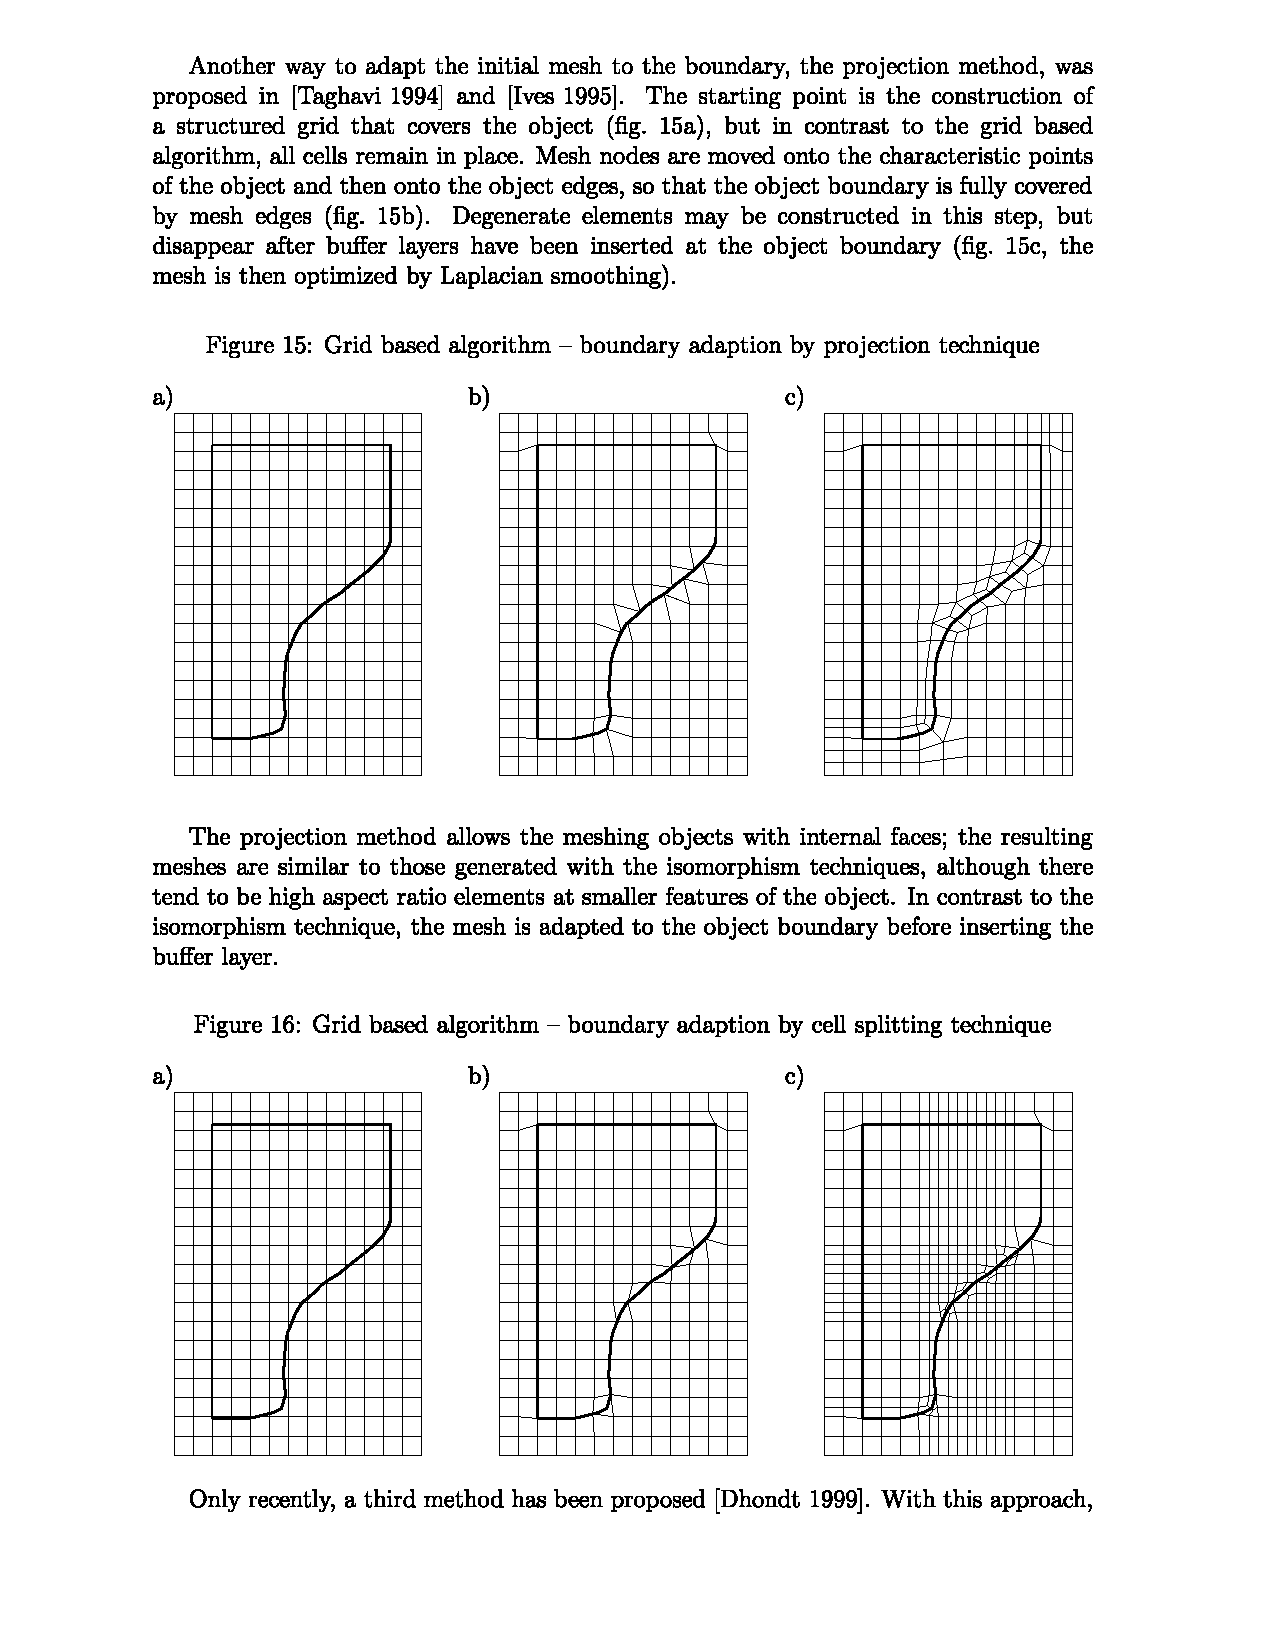
\includegraphics[width=0.325\linewidth]{grid}
}
\subfloat[初始]{
\includegraphics[width=0.325\linewidth]{init}
}
\subfloat[结果]{
\includegraphics[width=0.325\linewidth]{final}
}
}
\vspace{-2mm}
\caption{可视化例子1中的各向异性。 (a) 在定义域中的目标各向异性,使用椭圆来表示。 (b) 初始网格上的$H_\tau$。 (c) 收敛后的$H_\tau$。 结果上的各向异性和目标很接近。}
\label{fig:2daniso}
\vspace{-3mm}
\end{figure}

\begin{figure}[!h]
\centerline
{
\subfloat[BAMG]{
\includegraphics[width=0.37\columnwidth]{fem++_tanh}
}
\subfloat[LCT]{
\includegraphics[width=0.37\columnwidth]{ours_tanh}
}
}
%\vspace{-2mm}
\centerline
{
\subfloat[BAMG]{
\includegraphics[width=0.37\columnwidth]{fem++_cos_x2_y2}
}
\subfloat[LCT]{
\includegraphics[width=0.37\columnwidth]{ours_cos_x2_y2}
}
}
%\vspace{-2mm}
\caption{例子2 -- 与BAMG进行比较。 黎曼度量诱导于非凸解析函数$u(x,y) = \tanh( 10(\sin(5y) -2x)) + x^2 y + y^3$ (上面一行) 和$u(x,y) = e^{3\cos \frac{x^2+y^2}{5}}$ (下面一行)的Hessian矩阵,输入定义域是$[-5.5,5.5]^2$,各向异性比例的范围分别是$[1.9,394.4]$和 $[5.4,597.8]$。 网格三角形的颜色是由面积质量$\qarea$决定的。
}\label{fig:tanh}
\vspace{-3mm}
\end{figure}

我们同时和Zhong等的基于粒子的方法~\cite{Zhong2013}进行比较。对于核函数的宽度值,我们使用了他们推荐值$\sigma$,并且为了实验,选择了两个不同的粒子搜索范围$5\sigma$和$20\sigma$。基于粒子的方法的平均三角形质量比ODT或者LCT差,并且最差的三角形质量($\qtrimin$)远远低于ODT或者LCT。图~\ref{fig:exp}(d)(e)中的颜色也展示了比较差的面积质量。基于粒子的能量只惩罚了粒子之间的黎曼距离的不规则性,但是忽略了三角形之间的关系。

最后, 我们还和Chen的基于ODT的局部区域方法(local patch)~\cite{Chen2004a}进行比较。 它首先在每个顶点$\mp$上,使用平均黎曼度量$\overline{\mathcal{M}}_\mp$构造了一个凸二次函数$u(\mx) = \mx^T \, \overline{\mathcal{M}}_{\mp} \, \mx$。$\overline{\mathcal{M}}_\mp$是在它的一领域中计算的。然后它通过优化局部ODT能量$\int_{\Omega_{\mp}} |u(\mx)-\hat{u}(\mx)|\, \mathrm{d} \mx$,来一个一个的更新每个顶点$\mp$。 如果这个方法使用了局部二次函数,所以与我们的算法相比,会出现相似的结果。但是它没有考虑顶点更新而给其他顶点带来的影响。这个算法有可能不收敛或者收敛到一个不是最优的各向异性网格。图~\ref{fig:exp}(f)展示了~\cite{Chen2004a}的结果,它没有很好的符合指定的各向异性。相比于其他的方法,面积质量,ODT能量很差。 我们注意到将一个顶点周围的所有的局部ODT能量同时优化,~\cite{Chen2004a}结果可以提高。这其实是我们算法的一个变种,二次凸函数是定义在顶点上的,而不是定义在每个三角形上的。
图~\ref{fig:2daniso} 可视化了定义在输入网格和结果上的各向异性。

\textbf{例子2}\quad
图~\ref{fig:tanh}将我们的算法和BAMG进行比较。 BAMG是一个流行的程序,用来生成二维各向异性网格。我们选择了一个方形的区域作为定义域,并且测试了两个从非凸函数诱导的黎曼度量场。BAMG产生了质量比较低的结果,特别是在各向异性变化比较剧烈的区域。为了保证顶点的数目一致和比较的公平,我们将BAMG的输出作为我们的输入,然后使用LCT去优化,从而获得质量提高的结果(见表~\ref{tab:2d}中的质量统计值)。因此我们的算法能够很好的适应变化剧烈的黎曼度量场。

\begin{figure}[t]
\raggedleft
{
\subfloat[各向异性]{
\begin{overpic}[width=0.22\columnwidth]{strech20000}
\put(30,90){$\lambda(\mx)$}
\end{overpic}
}
\subfloat[particle]{
\begin{overpic}[width=0.26\columnwidth]{particle20000}
 \setlength{\fboxrule}{0.5pt}
 \setlength{\fboxsep}{0cm}
\put(12,50){\fbox{\includegraphics[width=0.1\columnwidth]{pzoom}}}
%\put(8,40){\small \contour{white}{zoomed-in view}}
\end{overpic}
\begin{overpic}[width=0.26\columnwidth]{particles}
 \setlength{\fboxrule}{0.5pt}
 \setlength{\fboxsep}{0cm}
\put(45,50){\fbox{\includegraphics[width=0.12\columnwidth]{pzoommesh}}}
%\put(8,40){\small \contour{white}{zoomed-in view}}
\end{overpic}
\begin{overpic}[width=0.22\columnwidth]{hist20000p}
\put(55,90){ $\qangall$}
\put(60,34){ $\qtri$}
\end{overpic}
}
}
\raggedleft
{
\subfloat[LCT]{
\begin{overpic}[width=0.26\columnwidth]{lcvt20000}
 \setlength{\fboxrule}{0.5pt}
 \setlength{\fboxsep}{0cm}
\put(12,50){\fbox{\includegraphics[width=0.1\columnwidth]{ourzoom}}}
%\put(8,40){\small \contour{white}{zoomed-in view}}
\end{overpic}
\begin{overpic}[width=0.26\columnwidth]{lcvt}
 \setlength{\fboxrule}{0.5pt}
 \setlength{\fboxsep}{0cm}
\put(45,50){\fbox{\includegraphics[width=0.12\columnwidth]{ourzoommesh}}}
%\put(8,40){\small \contour{white}{zoomed-in view}}
\end{overpic}
\begin{overpic}[width=0.22\columnwidth]{hist20000lcot}
\put(55,90){ $\qangall$}
\put(60,34){ $\qtri$}
\end{overpic}
}
}
%\centerline{\small
%(a) Stretch(x)  (b) Our point result  (c) Our mesh result  (d) Zhong \etal's point result (e) Zhong \etal's mesh result
%}
\caption{例子3 -- 和Zhong的基于粒子的方法~\cite{Zhong2013}法进行比较。 粒子法(b)和我们的方法(c) 使用了一个圆盘对称的各向异性比例$\lambda(\mx)$,显示在(a)中。 从左到右,我们比较了点的分布,面积质量$\qarea$,和角度质量与三角形质量的直方图。从点的分布与网格的局部放大的图,可以看出我们的结果变换的更加平缓,和指定的各向异性更加贴合,并且生成了更加规则的网格。我们的算法可以获得更好的角度质量$\qangall$(我们的结果更加聚在最优值60$^\circ$附近)和三角形质量$\qtri$(我们的结果更加聚在最优值1),可以直接从右端的直方图中体现。
}\label{fig:particlecompare2d}
\vspace{-3mm}
\end{figure}

\textbf{例子3}\quad
图~\ref{fig:particlecompare2d} 展示了另一个和Zhong的基于粒子的方法~\cite{Zhong2013}比较的结果。在定义域$[-100,100]^2$上,各向异性是通过一个圆盘黎曼度量场决定的:
$$\mathcal{M}(\mx) = Q(\mx) \, \diag(\lambda^2(\|\mx\|), 1) \, Q^T(\mx),$$
其中$\lambda \in [1,10]$,如图~\ref{fig:particlecompare2d}(a)所示。
20000个顶点在这个定义域内被采样,这个数目是来自~\cite{Zhong2013}的结果。 我们的算法使用了31秒,然而~\cite{Zhong2013}使用了20分钟左右。从图~\ref{fig:particlecompare2d}中的很容易看出,LCT获得了较好的结果,更好的顶点分布,更好的网格质量(同时见表~\ref{tab:2d})。

\textbf{例子4}\quad
LCT能量优化可以被认为是一种网格平滑,所以很自然的和其他的光滑函数优化进行比较。我们选择了三种流行的能量。
\begin{itemize}
\item 1.将所有的各向异性的边长的平方和累加:$E_1 \triangleq \sum |e_\Minv|^2$;
\item 2.将每个三角形的各向异性的边长的平方和用面积归一化后累加: $E_2 \triangleq \sum_\tau \frac{\sum_{\me \in \tau} |e_\Minv|^2}{|\tau|}$;
\item 3.将每个三角形的各向异性的边长的平方累乘用面积归一化后累加:$E_3 \triangleq \sum_\tau \frac{\prod_{\me \in \tau} |e_\Minv|}{|\tau|}$。
\end{itemize}
这三种能量都来自~\cite{Shewchuk2002}。
在顶点的更新和三角形网格边翻转中,将$E_1$, $E_2$ or $E_3$代替LCT能量。初始网格由我们的边长规则化策略产生。图~\ref{fig:energy}和表~\ref{tab:2d}显示了,相比于LCT能量,优化$E_1$或者$E_2$可以提高更小的网格质量,然而优化$E_3$反而降低了初始网格的质量。

\begin{figure}[t]
\centerline
{
\subfloat[initial mesh]{
\includegraphics[width=0.33\columnwidth]{input_mesh}
}
\hfill
\subfloat[optimizing $E_1$]{
\includegraphics[width=0.33\columnwidth]{energy_no_area}
}
\hfill
\subfloat[optimizing $E_2$]{
\includegraphics[width=0.33\columnwidth]{energy_divide_area}
}
}
%\vspace{-2mm}
\centerline{
\subfloat[optimizing $E_3$]{
\includegraphics[width=0.33\columnwidth]{energy_edgemul}
}
\qquad
\subfloat[optimizing LCT]{
\includegraphics[width=0.33\columnwidth]{energy_lcvt}
}
}
\vspace{-2mm}
\caption{例子四 -- 和其他的光滑函数比较。 黎曼度量是诱导于$u(x,y)=e^{\sin x + \cos y}$,各向异性比例范围是$[1,429]$。 网格最后使用面积质量$\qarea$着色。
}
\label{fig:energy}
\vspace{-3mm}
\end{figure}

\begin{table}[!h]
\caption{例子2,3,4的质量统计。}
\centering \scalebox{0.9}{
\begin{tabular}{lrcccc}%|l}
  \toprule
  % after \\: \hline or \cline{col1-col2} \cline{col3-col4} ...
   &\#vert & $\lambda$&$\qtrimin/\qtriavg/\qtridev$ & $\qangmin/\qangavg/\qangdev$ & $r_6$ \\% & $r_\angle$   \\
   \midrule
  Fig.~\ref{fig:tanh}a (BAMG)  & 1289 &[1.9,394.4]& 0.22/0.83/0.13 & $10.3^\circ/46.4^\circ/8.9^\circ$ & 0.60 \\%& 0.31 \\
  Fig.~\ref{fig:tanh}b (LCT)  & 1289 &[1.9,394.4]& \textbf{0.42}/\textbf{0.89}/\textbf{0.08} & $\textbf{22.8}^\circ/\textbf{50.4}^\circ/\textbf{5.8}^\circ$ & \textbf{0.69} \\%& \textbf{0.32} \\
   \midrule
  Fig.~\ref{fig:tanh}c (BAMG)  & 6251 &[5.4,597.8]& 0.07/0.87/0.08  & $3.9^\circ/49.6^\circ/6.0^\circ$ & 0.60 \\%& 0.19 \\
  Fig.~\ref{fig:tanh}d (LCT)  & 6251 &[5.4,597.8] & \textbf{0.45}/\textbf{0.90}/\textbf{0.07} & $\textbf{21.1}^\circ/\textbf{51.3}^\circ/\textbf{5.2}^\circ$ & \textbf{0.70} \\%& 0.19 \\
   \midrule
  Fig.~\ref{fig:particlecompare2d} (particle) & 20000 &[1,10] & 0.09/0.90/0.08 & $6.1^\circ/52.5^\circ/5.0^\circ$ & 0.78 \\%&0.19\\
  Fig.~\ref{fig:particlecompare2d} (LCT) & 20000 &[1,10]& \textbf{0.57}/\textbf{0.94}/\textbf{0.04} & $\textbf{31.0}^\circ/\textbf{54.5}^\circ/\textbf{3.3}^\circ$ & \textbf{0.90} \\%& \textbf{0.38} \\
   \midrule
  Fig.~\ref{fig:energy}a (init) & 2316 &[1,429] & 0.32/0.80/0.11 & $14.5^\circ/44.4^\circ/7.3^\circ$ & \textbf{0.67} \\%& 0.67 \\
  Fig.~\ref{fig:energy}b ($E_1$) & 2316 &[1,429]& 0.38/0.86/0.09 & $23.4^\circ/48.5^\circ/6.3^\circ$ & 0.40\\%& 0.77\\
  Fig.~\ref{fig:energy}c ($E_2$) & 2316&[1,429] & 0.42/0.87/0.08 & $25.4^\circ/49.4^\circ/5.6^\circ$ & 0.41 \\%& 0.80 \\
  Fig.~\ref{fig:energy}d ($E_3$) & 2316&[1,429] & 0.15/0.80/0.13 & $6.4^\circ/44.4^\circ/8.7^\circ$ & 0.38 \\
  Fig.~\ref{fig:energy}e (LCT) & 2316 &[1,429]& \textbf{0.60}/\textbf{0.91}/\textbf{0.06} & $\textbf{32.5}^\circ/\textbf{52.6}^\circ/\textbf{4.6}^\circ$ & 0.64 \\%& \textbf{0.84} \\
   \bottomrule
\end{tabular}
}
\label{tab:2d}\vspace{-4mm}
\end{table}

\subsection{三维各向异性曲面网格生成}
\begin{figure}[t]
\centerline
{
\includegraphics[width=1\columnwidth]{surf}
}
\vspace{-5pt}
\caption{使用我们的算法生成的各向异性三维曲面模型(Beetle, Rockarm 和 Hand)。}
\label{fig:nofeature}\vspace{-5mm}
\end{figure}

\begin{figure}[t]
\centerline
{
\begin{overpic}[width=1\columnwidth]{feature3}
%\put(22,6){\small angle}
%\put(56,6){\small angle}
%\put(90,6){\small angle}
\end{overpic}
}
\vspace{-5pt}
\caption{使用我们的算法应用到带有尖锐特征的各向异性曲面网格生成中(Block, Impeller 和 Fandisk)。  }\label{fig:feature}\vspace{-5mm}
\end{figure}

图~\ref{fig:nofeature}展示一些曲面的结果(Beetle, Rockarm, Hand 模型),各向异性是通过曲面的曲率决定的。 对于这三个模型,我们的方法分别使用64, 17 和77秒生成高质量的结果(见表~\ref{table:stat})。我们将LCT应用到有尖锐特征的曲面上,如图~\ref{fig:feature}所示。

\begin{figure}[t]
\centerline
{
\begin{overpic}[width=1\columnwidth]{cyclide}
\put(25,7){ $\qangall$}
\put(59,7){ $\qangall$}
\put(93,7){ $\qangall$}
\end{overpic}
}
\centerline
{
\textbf{(a)} ACVT \hspace{0.15\linewidth} \textbf{(b)} particle \hspace{0.15\linewidth} \textbf{(c)} LCT
}
\caption{在Cyclide模型上,和ACVT~\cite{Valette2008}与基于粒子的方法~\protect\cite{Zhong2013}进行比较。从放大的局部图和直方图来看,我们的结果要远好于它们。
%\jms{Hard to see whether the angular histogram is an better for us than Zhong.}
%\jms{Center labels!}
}\label{fig:cyclide}
\vspace{-3mm}
\end{figure}

图~\ref{fig:cyclide} 将我们的算法和ACVT~\cite{Valette2008}, 基于粒子的方法~\cite{Zhong2013}在Cyclide模型上进行比较。ACVT生成了很差的结果:$16.8\%$ 的三角形拥有小于$30^\circ$的角。基于粒子的算法稍微好点,但是相比于我们,质量还是差了很多。比如我们的度为6的顶点比例,基于粒子的算法和ACVT分别为: 0.87,0.78,0.51。同时我们能获得更好的三角形和角度质量,见表~\ref{table:stat}中更多的数据。

\begin{figure}[!h]
\centerline
{
\begin{overpic}[width=1\columnwidth]{Fertilitynew}
\put(20,51){  ACVT}
\put(65,51){  ADR}
\put(20,-3){  particle}
\put(65,-3){  LCT}
\end{overpic}
}
\vspace{3mm}
\caption{和ACVT~\protect\cite{Valette2008},基于粒子的方法~\protect\cite{Zhong2013}, 与ADR~\protect\cite{Boissonnat2013} 在模型Fertility上比较。放大的局部图很好的展示结果的差别,说明我们的方法能获得更好质量的结果。 }
\label{fig:fertility}
\vspace{-3mm}
\end{figure}

\begin{table}[t]
\caption{生成各向异性曲面网格的质量和时间统计。我们列出了参考网格的顶点数目(“ref \#vert”),初始网格的顶点数目(“init \#vert”),输出网格的顶点数目(“\#vert”)。$\lambda$是各向异性比例的范围。$\%_{<30^{\circ}}$是三角形的最小角小于$30^\circ$的比例。$\dis_{H}$是参考网格与输出网格之间的Hausdorff距离与参考网格包围盒的对角线长度之间的比例。对于ACVT方法,参考网格被细分用来提供更好的近似精度。基于粒子的方法和ADR的数据是来自于\protect\cite{Zhong2013}。
}
\centering \scalebox{0.6}{
\begin{tabular}{lrrrcccrccr}%|r}
\toprule
模型               & ref \#vert & init \#vert & \#vert & $\lambda$ & $\qtrimin/\qtriavg/\qtridev$ & $\qangmin/\qangavg/\qangdev$ & $\%_{<30^{\circ}}$ & $\dis_{H}$ & $r_6$ %& $r_\angle$
& time (s) \\
\midrule
Cyclide (particle) & -     & 8000   & 8000   & $[2, 29]$  & 0.09/0.87/-      & $5.03^\circ/49.7^\circ/-^\circ$   & \textbf{0.04}\%   & 4.4e-4        & 0.78 %& 0.06
& 155.8             \\
Cyclide (ACVT) & 414720    & 8000    & 8009    & $[2, 29]$ & 0.002/0.75/0.17  & $0.07^\circ/40.8^\circ/10.8^\circ$   & 16.8\%            & 3.6e-3         & 0.51 %& 0.26
& 177.0             \\
%Cyclide (ACVT) & 414720    & 8000    & 8000     & ?      & ?      & $?^\circ$   & $?^\circ$   & ?\%            & $?\times10^{-2}$         & 0.46 & ?      & 154.3             \\
Cyclide (LCT)     & 25920     & 8000   & 8000    & $[2, 29]$  & \textbf{0.60}/\textbf{0.92}/\textbf{0.05}
    & $\textbf{26.9}^\circ/\textbf{53.1}^\circ/\textbf{4.2}^\circ$   & \textbf{0.03}\%            & \textbf{3.4e-4}       & \textbf{0.87} %& \textbf{0.35}
         & \textbf{17.5}         \\
\midrule
Fertility (ACVT) & 223626     & 12480   & 12480   & $[1, 14]$   & 0.00/0.67/0.19      & $0.12^\circ/35.6^\circ/11.7^\circ$   & 32.67\%            & \textbf{1.1e-3}        & 0.39 %& 0.57
      & 37.5             \\
%Fertility (ACVT) & 223626     & 12480   & 12480     & 0.002      & 0.67      & $0.12^\circ$   & $35.6^\circ$   & 32.67\%            & $1.1\times10^{-3}$         & 0.26 & 0.57        & 58.8            \\
Fertility (ADR) & -     & 12480   & 12480   & $[1, 14]$   & 0.002/0.56/-      & $0.06^\circ/29.9^\circ/-^\circ$   & 41.79\%            & 5.8e-3       & 0.46 %& 0.38
    & - \\
    %& {\raise.17ex\hbox{$\scriptstyle\sim$}}400            \\
Fertility (particle) &-   & 12480     & 12301  & $[1, 14]$    & 0.02/0.70/-      & $0.86^\circ/37.6^\circ/-^\circ$   & 26.99\%            & 2.3e-3          & 0.49 %&  0.28
 & \textbf{10.0}           \\
Fertility (LCT)     & 13971   & 12480     & 12480  & $[1, 14]$   & \textbf{0.54}/\textbf{0.89}/\textbf{0.07}
& $\textbf{24.9}^\circ/\textbf{50.8}^\circ/\textbf{5.1}^\circ$   & \textbf{0.04}\%           & \textbf{1.1e-3}      & \textbf{0.68} %&\textbf{0.65}
& 66.8         \\
\midrule

Rockarm               & 9413  & 1272       & 5550  & $[1, 18]$    & 0.34/0.86/0.08      & $20.4^\circ/48.9^\circ/6.1^\circ$   & 0.46\%             & 1.8e-3       & 0.60 %& 0.63
   & 17.6           \\
Fandisk             & 6475    & 1927     & 7950   & $[1, 15]$   & 0.14/0.87/0.08      & $8.4^\circ/48.9^\circ/5.8^\circ$   & 0.18\%             & 9.5e-4       & 0.60 %&  0.51
   & 19.6           \\
Beetle            & 17908      & 17908      & 9817   & $[1, 15]$   & 0.27/0.87/0.08      & $13.2^\circ/48.9^\circ/6.0^\circ$   & 0.66\%     & 9.2e-4    & 0.52 %& 0.53
&   64.3  \\
Block               & 8052    & 3307     & 11667  & $[1, 15]$    & 0.51/0.88/0.07      & $27.2^\circ/50.1^\circ/5.4^\circ$   & 0.03\%             & 1.1e-3        & 0.63 %& 0.66
   & 38.7           \\
Impeller            & 10000  & 10000      & 11737   & $[1, 16]$   & 0.39/0.87/0.08      & $22.1^\circ/49.6^\circ/5.8^\circ$   & 0.17\%             & 6.5e-4      & 0.60 %& 0.40
    & 110.5          \\
Botijo              & 14989   & 700     & 13890  & $[1, 16]$    & 0.52/0.89/0.07      & $23.1^\circ/50.9^\circ/5.0^\circ$   & 0.04\%             & 1.6e-3      & 0.66 %& 0.75
    & 39.1         \\
Hand                & 30000  & 2576     & 21226  & $[1, 14]$   & 0.46/0.90/0.06      & $20.6^\circ/51.4^\circ/4.8^\circ$   & 0.04\%             & 1.1e-3    & 0.67% & 0.60
     & 77.1          \\
%Buddha        & 115474    & 5000   & 63284  & $[1, 34]$ & 0.41/0.88/0.07  & $17.4^\circ/49.9^\circ/5.4^\circ$   & 0.03\%           & 6.7e-4      & 0.64 %& 0.56 & 178.5         \\
%Lucy                & 262787    & 74119  & 255097   & $[1, 19]$   & 0.26/0.90/0.06      & $15.4^\circ/51.4^\circ/5.0^\circ$   & 0.04\%             & 3.9e-4    & 0.70% & 0.60  & 2766.0          \\
\bottomrule
\end{tabular}}
\label{table:stat}\vspace{-5mm}
\end{table}

\begin{figure}[b]
\centerline
{
\begin{overpic}[width=0.95\columnwidth]{planar}
\put(93,74){  $\qangall$}
\put(93,55){  $\qre$}
\put(33,40){MMG3D}
\put(93,30){  $\qangall$}
\put(93,12){  $\qre$}
\put(35,0){LCT}
\end{overpic}
}
\vspace{2mm}
\vspace{-8pt}
\caption{简单的各向异性四面体网格生成例子。黎曼度量场是$\mathcal{M}(\mx)=\Lambda^2(\mx)$,其中$\Lambda(\mx) = \diag\left((0.0025+0.2(1-e^{-|x-0.6|}))^{-1}, 5, 5 \right)$。
中间的图像是四面体网格的切面图,展示了内部四面体的情况。右边的图像是所有的二面角$\qangall$和半径-边长比例$\qre$的直方图。我们的算法提供了离最优值(70.5$^\circ$ 对于 $\qangall$, 0.61 对于 $\qre$)更紧的分布。
}\label{fig:planartet}
\vspace{-3mm}
\end{figure}

图~\ref{fig:fertility} 将我们的算法和ACVT~\cite{Valette2008},基于粒子的算法和ADR~\cite{Boissonnat2013}在Fertility模型上进行比较。目标的黎曼度量是由曲面的曲率决定的。基于粒子的算法跑了100次迭代,并且使用并行进行加速。目标输出的顶点数目是和ADR的输出一致的。我们的算法可以获得更好的网格正则度,对原始的网格的近似更加合理(见表~\ref{table:stat}中的Hausdorff距离)。对于角度和三角形质量,LCT获得了更好的质量,更好的贴合了到处的各向异性。

\subsection{各向异性四面体网格生成}

\begin{figure}[t]
\centerline
{
\begin{overpic}[width=0.95\columnwidth]{cylinder}
\put(93,74){  $\qangall$}
\put(93,55){  $\qre$}
\put(33,40){MMG3D}
\put(93,34){  $\qangall$}
\put(93,17){  $\qre$}
\put(35,0){LCT}
\end{overpic}
}
\caption{另外一个简单的体网格生例子,各向异性是类似圆柱变化的。黎曼度量是$\mathcal{M}(\mx)=\mQ^T(\mx) \, \Lambda^2(\mx) \, \mQ(\mx)$,其中$\Lambda(\mx) = \diag\left(2(0.1+2(1-e^{-0.01|x^2+y^2-49|}))^{-1}, 1, 1\right)$,$\mQ$的三列是 $(x/\sqrt{x^2+y^2}, y/\sqrt{x^2+y^2}, 0)^T$,
$(-y/\sqrt{x^2+y^2}, x/\sqrt{x^2+y^2}, 0)^T$和$(0,0,1)^T$。
}\label{fig:cylindertet} \vspace{-3mm}
\end{figure}

\begin{figure}[t]
\centerline
{
\begin{overpic}[width=0.95\columnwidth]{sine}
\put(93,65){  $\qangall$}
\put(93,48){  $\qre$}
\put(31,37){MMG3D}
\put(93,29){  $\qangall$}
\put(93,12){  $\qre$}
\put(33,0){LCT}
\end{overpic}
}
\caption{一个球内的正弦各向异性。黎曼度量是$\mathcal{M}(\mx)=\mQ^T(\mx) \, \Lambda \, \mQ(\mx)$,其中$\Lambda = \diag(1000,10,10)$, $\mQ$的三列是$(2\cos(6x),1,0)^T$和两个相互正交的向量。
}\label{fig:sinetet} \vspace{-3mm}
\end{figure}

\begin{figure}[t]
\centerline
{
\begin{overpic}[width=0.95\columnwidth]{bump}
\put(93,33){  $\qangall$}
\put(93,12){  $\qre$}
\end{overpic}
}
\caption{在一个复杂的bumpy形状中的圆柱各向异性。目标各向异性使用和图~\ref{fig:cylindertet}一样的$\mQ$,但是
$\Lambda_1(\mx) =1.2/(0.5 + 1 - e^{-0.05(x^2+y^2 - 2.56)}),\:
\Lambda_2(\mx)=\Lambda_3(\mx)=\Lambda_1(\mx)\,(1+5\sqrt{x^2+y^2})$。
}\label{fig:bump} \vspace{-3mm}
\end{figure}

图~\ref{fig:planartet}和~\ref{fig:cylindertet}将我们的算法和MMG3D相比。定义域是一个立方体$[0.1,1.1]^3$ (图~\ref{fig:planartet})或者$[1,11]^3$(图~\ref{fig:cylindertet})。两个结果的网格质量是类似的(见表~\ref{table:tetstat})。相比于MMG3D,从直方图与表中的统计信息可以看出我们的算法能够获得更好的角度和半径-边长比($\qre$)质量。并且网格质量的标准差也比MMG3D好。注意和MMG3D相比,我们的四面体网格拥有更加稀疏的四面体数量(1870顶点 vs. 2365 顶点在图~\ref{fig:planartet}中, 6338顶点 vs. 8217顶点在图~\ref{fig:cylindertet}中)。图~\ref{fig:sinetet}展示了另一个和MMG3D比较的例子,定义域是一个单位球,两个算法使用相同的表面作为输入。我们的算法可以生成更少的sliver四面体,更好的角度和半径-边长比质量。我们的算法比MMG3D慢,因为比较低效率的翻边实现,和串行的顶点更新。

我们在MMG3D的结果上,跑了100次迭代的LCT优化和一个最后的sliver四面体去除过程。结果同样被列在表~\ref{table:tetstat}中,命名为“MMG3D-LCT”。LCT能提高网格的角度和半径-边长比质量。

图~\ref{fig:bump}展示了一个更多体网格生成的结果。三维定义域是一个bumpy形状,各向异性是由一个解析函数决定的。 目标各向异性为
\begin{equation}
\Lambda(\mx) = \diag\left((0.025+(1-e^{-0.01|\|\mx\|^2-49|}))^{-1},1,1\right),
\end{equation}
$\mQ$的三列是$\mx/\|\mx\|$和两个相互正交的向量。 定义域是一个立方体$[1,11]^3$。

\begin{table}[t]
\caption{四面体各向异性网格生成的数据和时间统计。\#sliver$_b$和\#sliver$_a$是实施sliver四面体去除策略前与后的数量。}
\centering \scalebox{0.6}{
\begin{tabular}{lrrrcccrrr}
\toprule
Model & init \#vert & \#vert & \#tet & $\lambda$ & $\qangmin/\qangavg/\qangdev$ & $\qre_{max}/\qre_{avg}/\qre_{dev}$   & \#sliver$_b$ & \#sliver$_a$ & time (s) \\
\midrule
Fig.~\ref{fig:planartet} (LCT)    & 948   & \textbf{1870}  & \textbf{8144}  & $[1, 80]$  &$\textbf{24.7}^\circ/\textbf{51.7}^\circ/7.5^\circ$ &1.46/\textbf{0.76}/0.07  & 71  &  0   &   8.3  \\
Fig.~\ref{fig:planartet} (MMG3D)  & -     & 2365  & 10860 & $[1, 80]$  &$22.0^\circ/48.1^\circ/7.7^\circ$ &1.37/0.83/0.09  & -    &  0   &   \textbf{4.9} \\
MMG3D-LCT  & -     & 2365  & 10913 & $[1, 80]$  &$22.6^\circ/51.5^\circ/7.8^\circ$ &\textbf{1.36}/0.77/0.07  & 23    &  0   &   5.1 \\
\midrule
Fig.~\ref{fig:cylindertet} (LCT)  & 2226  & \textbf{6338}  & \textbf{31840} & $[1, 20]$  &$17.7^\circ/50.6^\circ/8.5^\circ$ &\textbf{1.54}/0.78/0.08  & 517  &  0   &   72.6 \\
Fig.~\ref{fig:cylindertet} (MMG3D)& -     & 8217  & 42067 & $[1, 20]$  &$16.2^\circ/46.8^\circ/8.2^\circ$ &2.59/0.86/0.13  & -    &  0   &   \textbf{15.4} \\
MMG3D-LCT  & -     & 8217  & 42435 & $[1, 20]$  &$\textbf{18.1}^\circ/\textbf{50.9}^\circ/8.6^\circ$ &1.71/\textbf{0.77}/0.09  & 530    &  0   &   31.2 \\
\midrule
Fig.~\ref{fig:sinetet} (LCT)      & 1966  & \textbf{4739}  & \textbf{22427}& $[1, 10]$  &$9.1^\circ/44.7^\circ/10.7^\circ$ &5.56/0.89/0.18   & 1715 &  72  &   103.8 \\
Fig.~\ref{fig:sinetet} (MMG3D)     & -     & 5187  & 25311& $[1, 10]$  &$6.2^\circ/37.1^\circ/10.9^\circ$ &6.27/1.21/0.41   & -    &  264 &   \textbf{6.5}  \\
MMG3D-LCT  & -     & 5187  & 25767 & $[1, 10]$  &$\textbf{9.4}^\circ/\textbf{44.8}^\circ/10.8^\circ$ &\textbf{3.50}/\textbf{0.88}/0.17  & 1932   &  \textbf{65}   &   33.1 \\
\midrule
%Fig.~\ref{fig:teaser}-right       & 2158  & 6554 & 32668 & $[1, 40]$  &$15.3^\circ/48.9^\circ/9.2^\circ$ &2.80/0.83/0.13   & 844   &  0  & 104.6 \\
Fig.~\ref{fig:bump}      & 18183  & 35096  & 153959 & $[1, 13]$  &$15.3^\circ/51.1^\circ/8.3^\circ$ &1.41/0.77/0.07   & 534  &  0   &   339.4 \\
\bottomrule
\end{tabular}}
\label{table:tetstat} \vspace{-3mm}
\end{table}

\section{本章小结}
局部凸函数三角化(LCT)提供了一个新颖的、简单的算法来生成二维平面区域,三维曲面区域和三维体区域上的高质量各向异性网格。我们的算法继承了ODT的优点,并且推广它能适用于一般的黎曼度量场。它提供了高效率和极好的网格质量。当然我们的算法存在一些局限性,供未来的工作来解决。

\paragraph{网格质量的界}
与\cite{Labelle2003,Boissonnat2008a}相比,我们不能对网格质量提供严格保证。一个可能的解决思路是结合\cite{Boissonnat2008a}的各向异性Delaunay细化和我们的LCT优化,来给最坏的网格质量提供界限,并且保持我们算法的平均质量。另外最小化最大误差$E_{LCT,\infty}$也是另外一个思路来控制最差质量。

\paragraph{凸局部函数}
和Chen等的方法~\cite{Chen2007}一样,我们的方法通过公式~\ref{eqn:funcmetric}将一个负定的Hessian矩阵转换成正定。当函数$u$是局部非凸时,我们的方法会降低对原始函数的逼近程度。应该使用一个更一般的,而不是公式~\ref{eqn:u_tau}中的$H$。这样一个一般的LCT形式能提供更高的逼近程度,但是会使得优化更加复杂。另外一个可能性是将二次凸函数换成一个更一般的凸函数,能够更好地匹配局部黎曼度量,比如Bernstein-B\'{e}zier样条。




  %\chapter{快速鲁棒的多立方体结构生成} \label{chap:polycube}
输入一个四面体网格$\mM$,本章目标是从$\mM$出发,构造一个奇异性可控的多立方体结构和一个低形变的体映射。对于曲面输入,本章使用TetGen软件~\cite{Si2015}将它们四面体化。在~\ref{sec:deform}节中我们优化表面三角形法向的光滑和对齐能量来驱动网格变形和自动去除极限点。在~\ref{sec:label_and_flatten}节中我们给出如何对网格的表面三角形进行标记,如何确定当前的网格是不是拥有一个正确的多立方体拓扑结构,以及如何使用保证无翻转的算法将网格严格压平,而得到最终的多立方体结构。

\section{网格变形} \label{sec:deform}
我们设计了三个能量函数项来驱动网格变形(~\ref{sec:obj}节):法向光滑能量,法向对齐能量和刚性形变函数~\cite{Fu2015}。在最小化的过程中,我们动态地调节上述能量函数中的比例参数,将输入网格变形成多立方体结构(~\ref{subsec:smooth} 和~\ref{subsec:align}节)。在\ref{subsec:minimize}节中,描述了如何高效地优化上述的能量函数。

\subsection{目标函数设计} \label{sec:obj}
设输入网格为$\mM$,包含$N$个四面体$\{\mt_1,\ldots,\mt_N\}$,$N_v$个顶点$\{\mv^0_1,\ldots,\mv^0_{N_v}\}$,它的边界曲面网格是$\mathcal{S}$。$\mathcal{S}$包含$n$个面$\{\mf_1,\ldots,\mf_n\}$,它们的法向是$\{\mn_1,\ldots,\mn_n\}$。我们引入一个算子$\Ax(\cdot)$,它将一个三维向量映射到离它最近的轴方向上($(\pm 1,0,0)^T$, $(0,\pm 1,0)^T$ 或者 $(0,0,\pm 1)^T$), 比如,$\Ax ((3,2,1)^T) = (1,0,0)^T$。如果所有的面法向和轴方法能够完美的对齐,那么$\mn_i = \Ax (\mn_i), \forall \, i$。已经有方法利用法向与最近的轴$\Ax(\mn_i)$之间的距离来定义的能量,驱动网格的变形,同时将网格分割成块~\cite{Gregson2011}来生成多立方体结构。因为$\Ax(\mn_i)$操作算子具有过强的局部性质,直接使用可能会导致相邻法向之间的不一致性。为了避免直接使用$\Ax(\mn_i)$,本章使用高斯光滑后的法向来驱动变形。我们定义如下的\emph{法向光滑能量}。
\begin{equation} \label{eqn:smooth}
E_s = \sum_{i=1}^n \mu_i \cdot \| \mn_i - \Ax(G_\sigma(\mn_i)) \|^2.
\end{equation}
其中$\mu_i$是$\mf_i$上的权,$G_\sigma (\cdot)$是一个高斯函数:
\begin{equation}
G_\sigma (\mn_i) = \sum_{\mf_j \in \mF} \area(\mf_j)\,\exp\left(-\dfrac{\|\mp_{\mf_i}-\mp_{\mf_j}\|}{2\sigma_s^2} \right) \cdot \mn_j.
\end{equation}
其中$\mp_{\mf_i}$是面$\mf_j$的面心,$\|\mp_{\mf_i}-\mp_{\mf_j}\|$是从$\mp_{\mf_i}$到$\mp_{\mf_j}$的测地距离的简单近似,$\sigma_s$是高斯函数的核宽度,对于所有的$\mf_i$都是一样的。通过调节高斯函数的核大小,$E_s$能够改变最终多立方体结构的奇异性。

设$n^x, n^y, n^z$是一个法向的三个分量。 因为和轴对齐的法向有且仅有两个0分量,我们提出了如下的\emph{法向对齐能量}:
\begin{equation}
E_a = \sum_{i=1}^n \nu_i \cdot \left( (n_i^x \cdot n_i^y)^2 + (n_i^y \cdot n_i^z)^2 + (n_i^z \cdot n_i^x)^2 \right).
\end{equation}
其中$\nu_i$是$\mf_i$上的权。

由于我们希望输入网格和多立方体网格之间是尽可能一样的,于是需要考虑刚性形变。为了获得低形变的映射,我们使用了AMIPS能量~\cite{Fu2015}(第\ref{chap:AMIPS}章),它能惩罚最大的形变和防止翻转的或者退化的四面体。AMIPS通过如下的方式定义映射的刚性形变。设$\mA$ 是从输入四面体$\triangle \mv^0_p\mv^0_q\mv^0_r\mv^0_s$ 到变形四面体$\triangle \mv_p\mv_q\mv_r\mv_s$的仿射变换:
\begin{equation}
\mA = \left[\mv_p-\mv_q \,|\, \mv_p-\mv_r\,|\,\mv_p-\mv_s\right] \cdot \left[\mv^0_p-\mv^0_q \,|\, \mv^0_p-\mv^0_r\,|\,\mv^0_p-\mv^0_s\right]^{-1}.
\end{equation}
共形形变定义为:
\begin{equation}
\delta_{conf} = \frac{1}{8}\left(\|\mA\|^2_F \cdot \|\mA^{-1}\|^2_F -1\right),
\end{equation}
和体积形变定义为:
\begin{equation}
 \delta_{vol} = \frac{1}{2} \left(\det \mA + (\det \mA)^{-1} \right).
\end{equation}
这里的$\|\cdot\|_F$是Frobenius范数。将上述两个形变合并得到刚性形变,\emph{刚性AMIPS能量}定义为:
\begin{equation}
E_{iso} = \sum_{i=1}^N \exp \left( s \cdot \left(\alpha \, \delta_{conf} + (1-\alpha) \, \delta_{vol} \right) \right).
\end{equation}
在我们的方法中,我们设$s=1$和$\alpha = 0.5$。 很显然,当任何的四面体退化时,AMIPS能量会趋向于无穷。因为使用了指数函数,AMIPS能够非常有效的惩罚最大的形变和产生均匀的分布形变。

\textbf{目标函数}\, 我们将上述的能量函数合并得到多立方体变形能量:
\begin{equation}
E := E_{iso} + E_s + E_a.
\end{equation}
%其中$\mu_i,\nu_i$是$E_s$和$E_a$的权。%注意到模型的朝向会影响$E$的值,因此我们需要在顶点位置上引入了一个全局旋转矩阵$R$来减少目标函数。

如果我们能够最小化$E$(变量是网格$\mM$的顶点位置),并且使$E_a$达到0,就能自动地得到多立方体结构。但是由于$E$的高度非线性,直接优化$E$不能保证$E_a=0$满足。~\cite{Gregson2011,Livesu2013}方法中的思想是,首先将曲面网格分割成和轴对齐的块,然后将这些和轴对齐后的块严格压平。本文也是利用了这个思想。也就是说在网格变形的过程中,我们不需要做到完美的$E_a=0$,只需要能给每个$\mf_i$确定一个的标记(标记共有六种可能,即六个轴中的一个),使得整个网格表面的标记集是正确的(\emph{正确标记集}的定义见\ref{subsec:label}节)。在意识到上述优化的困难和整个表面只需要正确的标记集后,我们提出了如下的优化框架:
\begin{enumerate}
    \item \emph{法向光滑变形},设$\nu_i=0$,优化$E_{iso} + E_s$使得表面的法向和轴尽量对齐,这个过程和~\cite{Gregson2011}中旋转驱动的网格变形类似,所以会产生极限点;
    \item \emph{法向对齐变形},为了处理上述过程中出现的极限点,我们设$\mu_i=0$,优化$E_{iso} + E_a$使得出现在极限点附近的区域自动和轴对齐,因而可以自动的消除极限点;
    \item  检查上述优化是不是已经产生了正确的标记集,如果是就进行网格压平,否则回到步骤1进行迭代,直至产生正确的标记集。
\end{enumerate}
下面的章节将具体介绍上述的优化过程和参数($\mu_i,\nu_i$)的调节方法。

\subsection{法向光滑变形} \label{subsec:smooth}
这一步网格变形的过程中,我们希望映射是低形变的,同时让网格表面法向和轴尽可能的对齐。为了达到这个目标,需要一个自适应的$\mu$来维持$E_{iso}$和$E_s$之间的平衡,不让$E_{iso}$或者$E_s$来主导整个能量函数。当某个能量主导整个能量函数时,要么会导致法向和轴对齐不好,要么会产生很大的形变,这都会对后续的优化产生不好的影响。对于任意一个表面三角形$\mf_i$,有且仅有一个与之相邻的四面体$\mt_i$存在,这样的四面体称为边界四面体。$\mu_i$对于每个$\mf_i$ 是不同的。在网格变形前,$\mu_i$ 被定义为:
\begin{align}
%\begin{split}
\alpha_i &= \frac{E_{iso, i}}{E_{s, i}}, \\
\mu_i &= \min \left( \max \left( \alpha_i, \mu_{\min} \right) , \mu_{\max} \right),
%\end{split}
\end{align}
其中$E_{iso, i}$是变形前边界四面体$\mt_i$上的形变,$E_{s, i}$是变形前表面三角形$\mf_i$上的法向光滑能量。如果一开始形变比较小,这时计算得到$\alpha_i$比较小,优化的过程如果出现形变能量变大,法向光滑能量降低,会导致在后续优化中$E_{iso,i}$主导整个局部能量,使得表面三角形不能和轴对齐,因此需要最小值$\mu_{\min}$来截断,避免这种情况的出现。如果一开始的形变比较大,这时计算得到的$\alpha_i$ 比较大,因此后续优化中可能会出现数值不稳定,导致优化快速的陷入局部极小,所以使用$\mu_{\max}$来避免$\mu_i$太大。在我们的实现中,设$\mu_{\min} = 0.1 \cdot \lambda$和$\mu_{\max} = 2 \cdot \lambda$,其中$\lambda$是根据$\alpha_i$的平均值确定的。因为$E_{s, i}$的最小值是0,而$E_{iso, i}$的最小值是$e^s$,所以在计算$\alpha_i$时,太小的$E_{s, i}$会导致数值不稳定和太大的$\alpha_i$平均值;太大的$E_{s, i}$表明一开始法向和轴方向的差距很大,而最终目标是要和轴方法对齐的,假如这样的三角形用于估计参数,就会使计算出的$\alpha_i$ 的平均值偏小。所以我们需要使用$ \bar{\alpha} = \frac{1}{n} \sum_{i=1}^n \alpha_i$ 对$\alpha_i$进行过滤,选择$\alpha_i \in \left[ 2 \cdot \bar{\alpha}, 0.1 \cdot \bar{\alpha} \right]$。 使用过滤后的$\alpha_j$ 的平均值来确定$\lambda$:
\begin{equation}
\lambda = \min \left( \frac{1}{m} \sum_{j=1}^m \alpha_j , \lambda_{\max} \right),
\end{equation}
其中$\lambda_{\max} = 10^{16}$用来避免数值问题,$m$是过滤后$\alpha_j$的数量。

\subsection{法向对齐变形} \label{subsec:align}
为了优化$E_{iso} + E_a$,我们首先要消除模型朝向带来的影响,选取好的朝向让尽量多的表面三角形法向和轴对齐,因此在顶点位置上引入了一个全局旋转矩阵$R$来降低目标能量函数的值。目标函数中只有$E_a$是和$R$相关的,设所有的$\nu_i=1$得到$E_a$。选择欧拉角表示$R$,优化的时候只有三个变量(三个欧拉角),因此我们选用LBFGS 算法进行优化,速度非常快。将$R$应用到顶点位置上,就可以尽量降低模型朝向带来的影响。

\textbf{讨论1}\, 上述过程和~\cite{Huang2014}中的消除朝向带来的影响的做法是类似的。但是在我们的实验中,选择欧拉角表达$R$,而~\cite{Huang2014}使用九个数表示矩阵$R$,在优化中使用软约束来使$R$接近一个旋转矩阵。我们的做法更加直接、变量更少,能保证优化出来的$R$一定是旋转矩阵。

在消除了模型朝向带来的影响后,我们需要去优化$E_{iso} + E_a$,从而消除基于法向光滑能量的网格变形带来的极限点。在优化前,需要确定$\nu_i$。$\nu_i$的更新方式和$\mu_i$是类似,只是把$E_{s, i}$换成$E_{a,i}$。优化结束后,我们使用\ref{subsec:label} 节中的标记方法对每个$\mf_i$进行标记,如果整个网格拥有标记集,跳出网格变形步骤。

\subsection{优化算法} \label{subsec:minimize}
网格变形的过程是一个无约束非线性优化的过程。为了高效的优化,我们使用了\cite{Fu2015}中的非精确坐标块轮换下降算法,利用图着色算法进行并行加速。所以在更新一个顶点的时候,我们只需要实施一步梯度下降,计算效率比较高,同时使用回溯线搜索保证优化能量的下降和显式避免翻转四面体的出现。优化终止的条件是,能量收敛或者达到最大的迭代次数。和~\cite{Huang2014}相比,我们没有使用全局牛顿法类的优化算法,因此不需要计算整个能量函数的Hessian矩阵和通过求解线性系统来更新顶点,导致我们的算法的效率远远好于它。

\section{网格标记和压平} \label{sec:label_and_flatten}
和~\cite{Gregson2011,Livesu2013}的方法类似,在网格变形过程中,希望对整个网格表面三角形赋予正确的标记集而结束变形。在\ref{subsec:label}节中,讲明了如何对网格表面三角形进行标记,同时阐述了对于整体网格什么样的标记集是正确的。在拥有了正确的标记集后,在\ref{subsec:flatten}节中,首先鲁棒的计算每个表面三角形$\mf_i$上与对齐轴相容的目标位置分量,最后将网格压平,使表面严格的和轴对齐。

\subsection{标记} \label{subsec:label}
对于每个$\mf_i$,根据$\Ax(\mn_i)$的值,对变形后的网格表面进行标记,同时将拥有一样标记的相邻的三角形组成一个块$\mc_k$,这时能够得到初始的标记集$\mL_0$。设$\mc_k$的标记就是它里面的三角形的标记。$\mc_k$是多立方体结构的面,相邻的$\mc_i$ 和$\mc_j$ 的公共边是多立方结构的边$\me_k$,被多于2个$c_k$分享的原始表面网格顶点是多立方体结构的顶点$\mp_i$。不幸的是根据~\cite{Eppstein2010},对于标记好的表面网格,暂时没有找到充分必要的拓扑条件,来保证这个标记集肯定能导出多立方体结构。我们将~\cite{Eppstein2010} 中的准则作为充分条件来判断标记集的正确性,这和~\cite{Livesu2013}是类似的。准则如下:
\begin{itemize}
    \item 多立方体结构的任何一个面$\mc_k$的邻域数目不能少于4个;
    \item 多立方体结构的任何两个拥有相反朝向(比如+X与-X)的面不能共享一条边$\me_k$;
    \item 多立方体结构的任何顶点$\mp_i$的度为3。
\end{itemize}

在判断标记集$\mL_0$正确与否前,我们根据以下简单的准则对$\mL_0$进行如下操作。
\begin{enumerate}
\item 通过修改$\me_k$的邻域中三角形$\mf_i$的标记,尝试将每条$\me_k$拉直。如果$\mf_i$的三个相邻三角形的标记中有两个与$\mf_i$的不一样,就改变$\mf_i$的标记为那个不一样的标记。
\item 记$\mc_k$上的$\mf_i$的数目是$N_{\mc}$。如果$N_{\mc} < \epsilon_1$且$\mc_k$的邻域数目小于4,我们改变$\mc_k$的标记。如果$\mc_k$只有一个相邻块,那么它的标记直接改为相邻块的标记;相邻块的数目为2或者3的$\mc_k$,相邻块可以使用广度优先的算法将$\mc_k$的标记改变成自己的标记。如果$N_{\mc} \geq \epsilon_1$,那么直接判定$\mL_0$是不正确的。
\end{enumerate}

使用拉普拉斯光滑将每条$\me_k$进行平滑,将$\me_k$ 投影到它的期望方向上得到$\tilde{\me}_k$,$\tilde{\me}_k$经过$\me_k$的平均位置。如果$\tilde{\me}_k$存在拐点,那么它也是多立方体结构的极限点。$\me_k$的期望方向定义为与之相邻的$\mc_i$和$\mc_j$的标记对应的轴方向的叉积,叉积的顺序对寻找极限点没有影响。
一个极限点的严重程度$S$定义为一个三角形的面积,这个三角形的三个顶点是极限点本身,$\me_k$上离极限点最近的两个其他的极限点或者多立方体结构的顶点。

如果所有$S<\epsilon_2$且$N_{\mc} < \epsilon_1$,并且同时满足上面提到的三个准则,则这时的标记集是正确的。其中$\epsilon_1$和$\epsilon_2$是两个阈值,在我们的实现中,$\epsilon_1 = 5$,$\epsilon_2 = 3 \cdot \frac{1}{n} \sum_{i=1}^n \area(\mf_i)$。

\subsection{压平} \label{subsec:flatten}
虽然经过上面的操作,我们能够得到正确的标记集,但是这时网格表面还没有和轴严格的对齐。多立方体结构中每个$\mc_k$上表面网格顶点位置中有一个分量是一样的,并且这个分量是和$c_k$的标记相容的,设它的值为$v_k$。为了压平网格的表面,我们需要首先确定每个$\mc_k$上的$v_k$,这样就定义了最终的多立方体结构的表面位置约束,然后利用第\ref{chap:affine}章中保证无翻转的算法在满足约束的前提下,将网格变形成多立方体结构。当网格(二维或者三维)的边界映射是一一映射的时候,没有翻转的网格单元的映射是一个一一映射~\cite{Lipman2012,Aigerman2013}。所以在计算映射的时候,首先计算$\me_k$的映射(一维),其次是$\mc_k$的映射(二维),最后才是整个网格的映射(三维)。这样我们能够生成无翻转的映射,甚至是一一映射。最终的映射不是双射的原因是,网格不同部分可能存在相交,但是这种情况对于某些应用而言是无所谓的,比如六面体网格生成。

我们利用如下的二次规划算法寻找每个$\mc_k$的$v_k$:
\begin{equation} \label{equ:QP_flatten}
\begin{split}
    \min \   &\sum_{v_i} (v_i - m_i)^2 \\
      s.t. \ &v_j - v_k > l_{j,k},
\end{split}
\end{equation}
其中$m_i$是$\mc_i$上顶点坐标值中和轴相容的平均值,约束描述的是某些配对的$\mc_j$和$\mc_k$需要满足的要求。一旦优化问题\ref{equ:QP_flatten}没有解,我们会通过$l_{j,k} = 0.8 \cdot l_{j,k}$缩短$l_{j,k}$直至收敛。

为了寻找配对的块($\mc_j$,$\mc_k$),确定它们之间的前后顺序约束和距离约束$l_{j,k}$,我们使用下面的两个准则:
\begin{enumerate}
\item 多立方体结构的每条$\me_k$ 的端点被三个块共享,去除和$\me_k$相邻的两个块,两个端点处剩下的块构成配对的块。将两个端点在$\tilde{\me}_k$上的位置之差设为$l_{j,k}$,很容易能做到$l_{j,k}>0$,这样块之间的顺序约束也能确定;
\item 在每个块$\mc_i$上,寻找到平行的多立方体结构的边集合,两两组合成配对的边。如果可以使用多立方体结构的边将配对的边连接起来,我们去除这个配对的边;如果配对的边之间没有公共部分,也被去除掉。在配对的边($\me_j$,$\me_k$)相邻的块中,有一个块是一样的,就是$\mc_i$,将剩下两个不同的块组成配对的块($\mc_j$,$\mc_k$)。$l_{j,k}$通过$\tilde{\me}_j$和$\tilde{\me}_k$之间的公共区域的平均距离决定的,同样强制$l_{j,k}>0$。
\end{enumerate}
\textbf{讨论2:}\, 和~\cite{Gregson2011}类似,我们利用变形后的网格位置和正确的标记集来寻找配对的块,块之间的前后顺序和距离约束。但是和~\cite{Gregson2011}的不同点是,我们将这些约束设为硬约束,能够保证生成合理的$v_k$,然而~\cite{Gregson2011}只是将它们作为软约束,不能保证之前定义的顺序和距离约束。

对于六面体网格生成的目标,$v_i$应该是目标方格长度(用户定义)的整数倍。所以我们会将优化问题\ref{equ:QP_flatten}中的$m_i$四舍五入成方格长度的整数倍。不等式的右端被设成$l_{j,k}$和方格长度的最大值,用来避免产生退化的四面体。\ref{equ:QP_flatten} 优化结束后,我们将$v_i$ 四舍五入成方格长度的整数倍。因为使用了硬约束的优化,我们能鲁棒的产生具有不同方格长度的六面体网格,如图\ref{fig:diff_resolution_hex}所示。

\section{实验与比较} \label{sec:pc_results}
我们的实验是在一个拥有英特尔3.4\,GHz CPU和16\,GB RAM的台式机上运行。为了产生无翻转的结果,输入的四面体网格需要满足,没有任何内部边或者面的所有顶点都在边界上\cite{Aigerman2013}。在我们的实现中,我们将这些边和面劈开,生成合理的输入网格。使用和第\ref{chap:AMIPS},\ref{chap:affine}章一样的形变定义来度量映射的好坏,主要是刚性形变。

\subsection{无翻转的四面体}
在后续的应用中,多立方体结构中翻转的四面体会导致其他算法的失败。比如在六面体网格生成中,如果一个六面体网格单元的顶点在一个翻转的四面体中,它反投影回原始网格中的位置是不明确的,存在二义性。图\ref{fig:flipped_cmp}中给出了和~\cite{Huang2014} 的比较,我们算法能生成无翻转,并且低形变的多立方体结构。在~\cite{Huang2014}和~\cite{Gregson2011}中,使用的能量是基于四面体与顶点的尽量刚性(ARAP)能量,它们都没有能力保证没有翻转的单元出现,比如~\cite{Gregson2011} 中的图9。

\begin{figure}[t]
\centerline
{
\begin{overpic}[width=0.99\columnwidth]{Polycube/flipped_cmp}
\put(15,-3){\textbf{(a)}}
\put(50,-3){\textbf{(b)}}
\put(88,-3){\textbf{(c)}}
\end{overpic}
}
\vspace{4mm}
\caption{多立方体映射中有无翻转的比较。(a) 原始的大象模型。(b)~\cite{Huang2014}的方法生成的结果,存在592个翻转的四面体,使用黄色表示。(c)我们的算法生成的无翻转四面体的多立方体结构,它最大的刚性形变是10.46。}
\label{fig:flipped_cmp}
\vspace{-3mm}
\end{figure}

在优化问题\ref{equ:QP_flatten}中,我们使用了硬约束来表达不同块之间的前后顺序和距离约束,所以$v_k$的求解是非常鲁棒的。如果不使用我们的算法,两个相邻平行的块($\mc_i$,$\mc_j$),四舍五入它们的$v_i$和$v_j$可能会得到同一个值上,而导致出现退化的四面体。针对六面体网格生成,我们可以提供具有不同方格长度的六面体结果(不是简单的细分后的不同分辨率)。图\ref{fig:diff_resolution_hex}展示了同一个模型上不同分辨率的六面体网格。目标方格长度分别为输入四面体网格表面边长的平均值的0.8倍(图\ref{fig:diff_resolution_hex}(b))和2.5倍(图\ref{fig:diff_resolution_hex}(c)),我们的方法都能成功的生成六面体网格。六面体网格的最小和平均缩放Jacobian行列式值分别为(0.410, 0.920)(图\ref{fig:diff_resolution_hex}(b))和(0.314, 0.822)(图\ref{fig:diff_resolution_hex}(c))。可以看到增加六面体网格的单元数量,可以在某些情况下提高整体网格的质量。图\ref{fig:diff_resolution_hex}(e) 和(f)表示的奇异性结构是一样的,也就是说这两个不同分辨率的六面体网格是来自同一多立方体结构。
\begin{figure}[t]
\centerline
{
\begin{overpic}[width=0.99\columnwidth]{Polycube/diff_resolution_hex}
\put(15,-3){\textbf{(d)}}
\put(50,-3){\textbf{(e)}}
\put(88,-3){\textbf{(f)}}
\put(15,32){\textbf{(a)}}
\put(50,32){\textbf{(b)}}
\put(88,32){\textbf{(c)}}
\end{overpic}
}
\vspace{4mm}
\caption{同一个模型产生不同分辨率的六面体网格。(a) 原始的Fertility模型。(d)我们的算法生成的无翻转四面体的多立方体结构。(b)和(c)是两个不同分辨率的六面体网格,分别拥有34302和2709个六面体。(e)和(f)分别是(b) 和(c) 的奇异性结构。因为不同的目标方格目标长度会要求两个多立方体结构,这里(d)只是展示了一个多立方体结构的作为代表,用于生成(b)。}
\label{fig:diff_resolution_hex}
\vspace{-3mm}
\end{figure}

\subsection{高效性}
在构造多立方体结构时,算法的效率是非常重要的,如果自动化的算法效率比较低,还不如直接使用人工进行设计。图\ref{fig:time_L1_cmp}展示了和~\cite{Huang2014}在同一个Kiss模型上构造多立方体结构的效率比较。图\ref{fig:flipped_cmp}(b)和(c)花销时间分别为23.4分钟,13.05秒。在这两个例子中,和~\cite{Huang2014}相比,我们都使用了接近一半的四面体数目的网格作为输入,虽然这样看上去有点不公平,但是我们的非精确的坐标轮换下降算法基本上是和四面体数目成正比的,也就是我们算法的时间大概也就是现在的两倍左右,这还是远低于~\cite{Huang2014}的时间。例外,我们根据~\cite{Livesu2013}的Kiss模型表面三角形网格生成四面体网格作为输入,共有442736个四面体,我们的算法大概花费了2.5分钟构造多立方体结构,1.5 分钟严格压平表面网格,其实我们的算法不需要这么多的四面体也能获得很好的结果。
我们的算法高效的原因如下,使用了高效的非精确坐标块轮换下降算法变形网格,同时不要求在开始的网格变形中严格压平所有的表面三角形而减少了迭代次数。而~\cite{Huang2014}使用了类似牛顿法进行优化,那么建立Hessian矩阵和求解线性系统的效率都很低。~\cite{Livesu2013}使用了启发式的局部搜索的策略消除极限点,同样效率比较低。

\begin{figure}[t]
\centerline
{
\begin{overpic}[width=0.99\columnwidth]{Polycube/time_L1_cmp}
\put(10,-3){\textbf{(a)}}
\put(35,-3){\textbf{(b)}}
\put(60,-3){\textbf{(c)}}
\put(90,-3){\textbf{(d)}}
\end{overpic}
}
\vspace{4mm}
\caption{Kiss模型上构造多立方体结构的效率比较。(a),(b)分别是~\cite{Huang2014}花了大约37.3分钟构造出的多立方结构,和对应的六面体网格。(a)图上平面上出现的瑕疵是翻转的四面体导致的。(c),(d)分别是我们的算法使用15.55秒生成的无翻转四面体的多立方体结构和对应的高质量六面体网格。}
\label{fig:time_L1_cmp}
\vspace{-3mm}
\end{figure}

\subsection{可控的奇异性}
用户可以根据某个参数的调节生成具有不同奇异性的多立方体结构。这种控制在某些应用是非常重要的,比如应用中奇异点数目和映射形变是相互矛盾的。我们的方法通过高斯函数的核宽度$\sigma_s$来控制奇异性。
图\ref{fig:diff_sigma_cmp}展示了在同一模型上,使用不同$\sigma_s$值来生成多立方体结构。从映射形变和奇异点的数目来看,大的$\sigma_s$可以生成更少的奇异点数目,更大的形变;小的$\sigma_s$能产生更多的奇异点数目,更少的形变。

\begin{figure}[t]
\centerline
{
\begin{overpic}[width=0.99\columnwidth]{Polycube/diff_sigma_cmp}
\put(10,-3){\textbf{(a)}}
\put(35,-3){\textbf{(b)}}
\put(60,-3){\textbf{(c)}}
\put(90,-3){\textbf{(d)}}
\end{overpic}
}
\vspace{4mm}
\caption{Buste模型上使用不同的$\sigma_s$来构造具有不同奇异性的多立方体结构。(a)原始Buste模型。(b),(c),(d)分别使用1,1.5,2.0倍平均输入表面网格的平均边长作为$\sigma_s$,分别生成具有128,72,36个奇异点的多立方体结构,平均刚性形变分别为1.50,1.53,1.57。}
\label{fig:diff_sigma_cmp}
\vspace{-3mm}
\end{figure}

\begin{figure}[t]
\centerline
{
\begin{overpic}[width=0.8\columnwidth]{Polycube/fertility_hex_cmp}
\put(20,50){\textbf{(a)}}
\put(62,50){\textbf{(b)}}
\put(20,-3){\textbf{(c)}}
\put(62,-3){\textbf{(d)}}
\end{overpic}
}
\vspace{4mm}
\caption{Fertity模型上使用不同的多立方体结构构造算法生成的六面体网格。(a),(b),(c),(d)分别来自\cite{Gregson2011},~\cite{Huang2014},~\cite{Livesu2013},我们的方法。六面体的数目分别是19870,53702,17910,24920。缩放Jacobian行列式的最小和平均值分别为(0.196,0.911),(0.260,0.872),(0.312,0.911),(0.422,0.917)。}
\label{fig:fertility_hex_cmp}
\vspace{-3mm}
\end{figure}

\subsection{六面体网格生成}
为了生成六面体网格,我们在生成多立方体结构的时候,已经将$v_k$都四舍五入成目标方格宽度的整数倍,因此可以直接将模型按照方格宽度进行缩放,使得所有的$v_k$变成整数。然后直接在整数点上直接建立六面体网格。最后将六面体网格的顶点根据它在四面体中的重心坐标反投影回输入网格区域,这样就得到了输入网格的六面体化。尽管在优化中,我们保证了无翻转,但是这只能保证每个六面体网格的顶点在一个四面体内,不能保证反投影后的六面体网格的缩放Jacobian行列式都大于0。 因此为了获得高质量的六面体网格,我们提出了如下的优化方法。

设反投影后的六面体网格为$\mM^H$。 首先在$\mM^H$的表面上插入一层~\cite{marechal2009,shepherd2007,Gregson2011}。为了去除拥有负的缩放Jacobian行列式的六面体(称为翻转的六面体),我们首先设计了一个简单的能量函数,通过优化它,能够生成无翻转的六面体。将一个六面体分成8个四面体,每个四面体的四个顶点是六面体的一个顶点$\mv_0^H$,在六面体上与$\mv_0^H$相邻的三个顶点$\mv_1^H$,$\mv_2^H$,$\mv_3^H$。对于每个四面体$\triangle \mv_0^H\mv_1^H\mv_2^H\mv_3^H$而言,将$\delta_{conf}$ 中的$\det(A)$变成$0.5 \cdot (\det(A) + \sqrt{\det(A)^2 + \zeta})$来定义新的能量,其中$\zeta$是一个比较小的正数,取法见~\cite{Escobar2003}。因此对于六面体网格而言,就是将8 个四面体上的能量相交。使用非精确坐标块轮换下降算法进行优化,效率很高。这个思想是和~\cite{Escobar2003,Sastry2014}类似的。虽然不能保证最后一定没有翻转的六面体,但是在实际中的效果很好。一旦没有翻转的六面体后,使用AMIPS~\cite{Fu2015}能量继续优化。为了获得更好的表面四边形,将\cite{Fu2014}中的LCT能量推广到四边形上,用于生成各向同性的表面四边形。通过交替表面四边形网格优化和内部顶点优化,能够获得很高的六面体网格质量。

图\ref{fig:fertility_hex_cmp}给出了一组都是使用多立方体结构来生成的六面体网格的比较。不管从缩放Jacobian行列式的数值统计,还是六面体网格表面上的颜色来看,我们的方法都能产生最好质量的六面体网格。图\ref{fig:LY_hex_cmp}比较了我们的六面体网格和~\cite{Li2012}的结果。图\ref{fig:LY_hex_cmp}(a)(b)的缩放Jacobian行列式的最小,平均值,六面体数目分别为:(0.293,0.940,133632), (0.336,0.947,59841);图\ref{fig:LY_hex_cmp}(c)(d)分别为(0.209,0.866,10600), (0.454,0.907,14606),所以我们的结果要好于~\cite{Li2012},同时图上六面体的颜色也反映了这个结论。

\begin{figure}[t]
\centerline
{
\begin{overpic}[width=0.8\columnwidth]{Polycube/LY_hex_cmp}
\put(24,40){\textbf{(a)}}
\put(70,40){\textbf{(b)}}
\put(24,-3){\textbf{(c)}}
\put(70,-3){\textbf{(d)}}
\end{overpic}
}
\vspace{4mm}
\caption{和~\cite{Li2012}比较生成的六面体网格。(a),(c)是~\cite{Li2012}的结果。(b),(d)是我们的结果。}
\label{fig:LY_hex_cmp}
\vspace{-3mm}
\end{figure}


\section{本章小结}
我们提出了一个自动构造多立方体结构的算法,首先通过网格变形找到正确的标记集,然后通过二次规划找到多立方体结构边界面的目标位置值,最后使用现有的保证无翻转的算法生成最终的多立方体结构。高斯平滑的核宽度是一个可调的参数,用来平衡映射的形变和多立方体结构的奇异性。通过将我们的算法应用一些模型上和进行六面体网格生成应用上,证明了算法能保证无翻转,高效性,奇异性可控等优点。同样,我们有一些局限性,需要在未来的工作中去解决。

\textbf{理论保证。} 对于任意输入的网格和任意的高斯平滑的核宽度,我们不能保证一定成功的生成合理的多立方体结构。对于寻找正确的标记集,没有理论保证能一定成功,因为我们使用了非线性优化算法来变形网格。在生成最终的多立方体结构的时候,因为使用的寻找无翻转的映射的技术,不能保证成功,导致我们的算法没有理论保证。

\textbf{高斯函数的核宽度}用来平衡映射形变和多立方体结构的奇异性。暂时,用户需要通过不停的尝试,才能找到一个最优的宽度。比如一些用户认为有兴趣的特征,相对与核宽度是很小的,导致最终的多立方体结构上不能体现。所以根据感兴趣的特征,设计一个空间变化的核宽度是非常有必要的。但是如何定义特征的尺度是一个非常有挑战的问题。我们想在未来进行这方面的尝试。

\textbf{多立方体结构的拓扑条件。} 我们使用的充分拓扑条件是一个强充分条件,暂时还没有弱充分条件出现。\cite{Huang2014}的结果中有度不是3的多立方体结构顶点产生,他们依然能产生正确的结构。同样在我们的实验中,如果将两个非常近的度为3的顶点合并成一个度为4的顶点也是可以的,注意为了最后产生无翻转的结果,度为4的多立方体结构顶点在原始网格表面上的度至少为6。所以在未来的工作中,寻找多立方体结构的充分必要拓扑条件是一个有趣课题。

  %\chapter{总结与展望} \label{chap:conclusion}
在科学研究、工程计算、文化娱乐中,三维数字模型扮演着越来越重要的角色。随着三维扫描技术和软件工具的发展,我们已经能很容易的获得这些三维数字模型。但是为了后续的应用,原始的数据一般不能被直接使用,需要进行相关的分析和处理,这个过程叫做\emph{数字几何处理}。本文研究的课题就是数字几何处理中的两个子课题,包括\emph{网格生成}和\emph{映射计算}。

\section{本文工作总结}
映射计算是计算机图形学中重要的基础课题,它可以被广泛地应用,比如平面网格参数化、网格变形、网格质量提高。\emph{最优映射}具有无翻转,低形变,计算效率高的性质。为了得到这样的映射,我们首先提出了AMIPS技术,它扩展了著名的MIPS 方法。AMIPS继承了MIPS保证无翻转性质,同时能显著地控制了最大的形变,显著地提高了计算效率。AMIPS的核心想法是,使用指数函数与MIPS能量结合,用于控制最大形变;使用非精确块坐标轮换下降算法进行优化,避免优化算法过早的陷入局部极小。但是AMIPS也存在局限性,比如不能处理带有大量控制点的网格变形,于是我们提出了基于组装分离的网格单元的最优映射计算,它首先能满足上述最优映射的要求,并且对初始映射,控制点的数目不敏感,同时可以计算形变有界的映射。它的基本出发点是将输入网格分离成不相连的网格单元,这时每个网格单元都是不翻转的,以每个网格单元上的仿射变换作为变量,建立一个无约束优化问题来组装分离的网格单元。在优化的过程中,保证网格单元上的映射一直满足无翻转、低形变的要求。在平面网格参数化、网格变形、网格质量提高等应用上的实验结果,相比于最先进算法我们算法具备很强的优越性。

各向异性网格在几何建模、物理模拟、机械工程等应用中,具有非常广泛的用途,可以提高数值模拟的精度。为了使网格生成算法能够适用于,一般化的黎曼度量场,同时适应各向异性变化剧烈的黎曼度量场和定义域网格中存在尖锐特征,我们提出了局部凸函数三角化(LCT)。LCT扩展了最优Delaunay三角化方法。LCT的关键思想是在每个网格单元上构造局部凸函数,它的Hessian矩阵局部上和输入的黎曼度量一致,使用网格顶点移动和改变网格连接关系的方法去降低函数逼近误差,生成满足输入的网格。在二维平面区域、三维曲面区域和三维体区域上生成的高质量各向异性网格证明了我们的算法能提供极高的计算效率和网格质量。

多立方体结构是一种特殊的网格结构,网格表面三角形的法向是($(\pm 1,0,0)^T$, $(0,\pm 1,0)^T$ 或者 $(0,0,\pm 1)^T$)中的一个。多立方体结构能够被广泛地应用,比如六面体、四边形网格生成,纹理映射等。高质量的多立方体构造算法需要是自动的,映射无翻转,低形变,奇异性可控,算法效率高。我们提出了一种新颖的基于网格变形的算法,利用网格表面法向光滑与对齐的能量快速的构造多立方体结构。算法中的高斯函数的核宽度是一个可调的参数,用来平衡映射的形变和多立方体结构的奇异性。我们的算法应用到六面体网格生成中能生成无翻转,计算效率高,奇异性可控的多立方体结构。我们同时提出的六面体网格优化算法也可以显著地提高六面体网格的质量。

\section{未来工作展望}
虽然我们的算法都能够生成高质量的各向异性网格、低形变的映射和高质量的多立方体结构,但是它们都存在一个缺点,没有严格的理论保证,比如生成的各向异性网格没有质量的保证,最优映射的计算不能保证一定成功,多立方体结构的构造不能保证收敛。因此在接下来的研究中,我们希望能够从理论出发,在保证整体质量的前提下,开发出具备理论保证的算法。

最优映射的计算效率虽然现在已经很高,但是和基于线性的方法比较,还是比较慢。我们希望在未来的工作中能设计计算更快,形变更低的映射,比如对于大尺度的网格变形能够获得交互级别的反馈。另外双射在网格映射中具有很重要的地位,比如在纹理映射中,它能够提供图像和网格之间的一一映射。我们现在的算法主要针对局部单射的映射,如何计算有效的双射也是未来的研究方向。

因为四边形和六面体网格在有限元方法等应用中,具备计算精度高的优点,因此它们需要更加好的算法来生成。现在我们各向异性网格生成算法只能应用在三角形和四面体网格上,同时现在也存在很多的算法用来生成各向同性的四边形和六面体网格,所以我们希望在未来的工作去设计算法,将各向异性的概念推广到四边形或者六面体网格。

虽然现在我们提出了很高效的多立方体构造算法,用于生成六面体网格,但是最终的六面体网格在内部没有奇异性,导致奇异结构的形式比较单一,最终使六面体网格质量不够好。所以我们希望在构造好的多立方体结构上直接设计奇异结构来辅助生成更高质量的六面体网格。

最后,我们认为最优映射能够被更多的问题利用,不光是我们文中提到的问题。希望能有更多的问题可以利用最优映射的概念来实现以往不能实现的目标,使之在计算机图形学中能够广为流传。

  %自行添加
  %\include{chapter/...}

%%%%%%%%%%%%%%%%%%%%%%%%%%%%%%
%% 附件部分
%%%%%%%%%%%%%%%%%%%%%%%%%%%%%%
\backmatter

  % 参考文献
  % 使用 BibTeX
  % 选择参考文献的排版格式。注意ustcbib这个格式不保证完全符合要求,请自行决定是否使用

  \bibliographystyle{ustcbib1}%{GBT7714-2005NLang-UTF8}
  \bibliography{bib/tex1}
  %\nocite{*} % for every item
  % 不使用 BibTeX
  % %\renewcommand{\baselinestretch}{0.5}
\begin{thebibliography}{10}

\bibitem{deng:01a}
{邓建松,~彭冉冉,~陈长松邓建松,~彭冉冉,~陈长松邓建松,~彭冉冉,~陈长松邓建松,~彭冉冉,~陈长松邓建松,~彭冉冉,~陈长松邓建松,~彭冉冉,~陈长松邓建松,~彭冉冉,~陈长松邓建松,~彭冉冉,~陈长松邓建松,~彭冉冉,~陈长松邓建松,~彭冉冉,~陈长松邓建松,~彭冉冉,~陈长松}.
\newblock {\em \LaTeXe{}~科技排版指南}.
\newblock 科学出版社,~书号:~7-03-009239-2/TP.1516, 北京, 2001.

\bibitem{wang:00a}
王磊.
\newblock {\em \LaTeXe{}~插图指南}.
\newblock 2000.

\bibitem{zhang:03a}
张林波.
\newblock {\em 关于新版~CCT~的说明}.
\newblock 2003.

\bibitem{lshort-cn}
C\TeX{} 翻译小组.
\newblock {\em lshort~中文版~3.20}.
\newblock 2003.

\bibitem{knuth86e}
Donald~E. Knuth.
\newblock {\em Computer Modern Typefaces}, volume~E of {\em Computers and
  Typesetting}.
\newblock Addison-Wesley, Reading, Massachusetts, 1986.

\bibitem{knuth86d}
Donald~E. Knuth.
\newblock {\em {METAFONT}: The Program}, volume~D of {\em Computers and
  Typesetting}.
\newblock Addison-Wesley, Reading, Massachusetts, 1986.

\bibitem{knuth86c}
Donald~E. Knuth.
\newblock {\em The {METAFONT}book}, volume~C of {\em Computers and
  Typesetting}.
\newblock Addison-Wesley, Reading, Massachusetts, 1986.

\bibitem{knuth86b}
Donald~E. Knuth.
\newblock {\em {TeX}: The Program}, volume~B of {\em Computers and
  Typesetting}.
\newblock Addison-Wesley, Reading, Massachusetts, 1986.

\bibitem{knuth86a}
Donald~E. Knuth.
\newblock {\em The {TeX}book}, volume~A of {\em Computers and Typesetting}.
\newblock Addison-Wesley, Reading, Massachusetts, 1986.

\bibitem{lamport85a}
Leslie Lamport.
\newblock {\em {LaTeX} --- A Document Preparation System: User's Guide and
  Reference Manual}.
\newblock Addison-Wesley, Reading, Massachusetts, 2nd edition, 1985.

\end{thebibliography}


  % 附录,没有请注释掉
  %\begin{appendix}
  %  
\chapter{中国科学技术大学研究生学位论文撰写规范}
\label{chap:requires}
\section*{以下文字仅作示例,一切以学校规定为准!}
研究生院规定在此下载\url{http://gradschool.ustc.edu.cn/ylb/material/xw/wdxz/1.doc}

研究生学位论文集中反映研究生在研究工作中所取得的成果,代表研究生研究工作的水平,也是申请和授予相应学位的主要依据。为提高研究生学位论文的撰写质量,做到学位论文在内容和格式上的规范化,我们编写了《中国科学技术大学研究生学位论文撰写规范》,供申请学位的研究生参考执行。其中参考文献著录规则我们根据GB/T 7714-2005的标准撰写。硕士和博士学位论文除在研究深度等方面要求不同外,撰写要求基本一致。

\section{内容要求}

\subsection{封面} 
采用研究生院规定的统一封面,封面包含内容如下: 
\subsubsection{密级} 涉密论文必须在论文封面标注密级(内部、秘密、机密),同时注明保密年限。
\subsubsection{论文题目} 应准确概括整个论文的核心内容,简明扼要,最多不超过30字,必要时可以加副标题。
\subsubsection{作者姓名} 英文封面中按英文习惯书写,即名在前。姓名需写全拼。
\subsubsection{学科专业} 写所在专业的全称,不可用简写。
\subsubsection{导师姓名} 一般允许有两名指导教师,主要指导教师姓名写在第一位,后附其职称,次要指导教师排第二位,也需注明职称。
\subsubsection{完成时间} 填写论文打印成文的年月日。

\subsection{中国科学技术大学学位论文原创性和授权使用声明}
本部分内容使用统一的模版,具体内容见格式范例,提交时作者须亲笔签名。

\subsection{摘要和关键词}
\subsubsection{中文摘要}
摘要是论文内容的总结概括,应简要说明论文的研究目的、基本研究内容、研究方法、创新性成果及其理论与实际意义,突出论文的创新之处。不宜使用公式、图表,不标注引用文献。 
\subsubsection{中文关键词} 
关键词是为了文献标引工作从论文中选取出来用以表示全文主题内容信息的单词和术语,一般3--8个词,要求能够准确概括论文的核心内容。
\subsubsection{英文摘要与关键词}
以中文书写的论文,内容与中文摘要和关键词完全一致,其他语种书写的论文以简略为原则,不需要相同。

\subsection{目录}
目录页由论文的章、条、附录等序号、名称和页码组成。论文中如图表较多,可以分别列出清单置于目次页之后。图的清单应有序号、图题和页码。表的清单应有序号、表题和页码。

\subsection{符号说明}
如果论文中使用了大量的物理量符号、标志、缩略词、专门计量单位、自定义名词和术语等,应编写成注释说明汇集表。若上述符号等使用数量不多,可以不设此部分,但必须在论文中出现时加以说明。

\subsection{正文}
正文是学位论文的主体,包括绪论、论文主体及结论等部分。
\subsubsection{绪论}
内容应包括:选题的背景和意义,文献综述及研究现状,研究内容与预期结果,研究方法和实验设计,论文结构安排等。要求实事求是,不夸大、缩小前人的工作和自己的工作,言简意赅,突出重点,不与摘要雷同。
\subsubsection{论文主体}
论文主体是正文的核心部分,占主要篇幅,它是将学习、研究和调查过程中筛选、观察和测试所获得的材料,经过加工整理和分析研究,由材料而形成论点。由于各学科及具体选题的差异,此部分不作统一规定。但总体内容必须实事求是,客观真切,准确完备,合乎逻辑,层次分明,简练可读。
\subsubsection{结论}
结论是对整个论文主要成果的总结,应明确、精炼、完整、准确。其中应明确指出本研究的创新点,对论文的学术价值和应用价值等加以预测和评价,说明研究中尚难解决的问题并提出今后进一步在本研究方向进行研究工作的设想或建议。

\subsection{参考文献}
本着以严谨求实的科学态度撰写论文,凡学位论文中有引用或参考、借用他人成果之处,均应详细列出所引文献的名称、作者、发表刊物、发表时间、卷号、页码等,严禁抄袭剽窃。  
\subsection{附录}
主要列入正文内过分冗长的公式推导,供查读方便所需的辅助性数学工具或表格,重复性数据图表,论文使用的缩写,程序全文及说明等。

\subsection{致谢}
对给予各类资助、指导和协助完成研究工作以及提供各种对论文工作有利条件的单位及个人表示感谢。致谢应实事求是,切忌浮夸与庸俗之词。

\subsection{在读期间发表的学术论文与取得的其他研究成果}
按学术论文发表的时间顺序,列齐本人在攻读学位期间发表或已录用的学术论文清单(发表刊物名称、卷册号、页码、年月及论文署名、作者排序)。其他研究成果可以是申请的专利、获得的奖项及完成的项目等。
 
\section{书写规定}

\subsection{论文的字数要求}
硕士学位论文要求不少于3万字,博士学位论文要求不少于5万字。

\subsection{文字、标点符号和数字}
除留学生和外语专业研究生外,学位论文一律用汉字书写。除非特殊需要,不得使用已废除的繁体字、异体字等不规范汉字。标点符号的用法以GB/T 15834—1995《标点符号用法》为准。数字用法以GB/T 15835—1995《出版物上数字用法的规定》为准。

留学生的学位论文所采用语种可以和导师商定,但论文封面须用中文。

\subsection{封面与扉页}
\subsubsection{秘级} 封面的秘级可以标注为内部、秘密和机密,各密级的保密时限分别为小于等于5年、小于等于10年和小于等于20年,非保密论文不标注密级。
\subsubsection{题目} 题目中避免使用缩略词、首字母缩写字、字符、代号和公式等。
\subsubsection{日期} 封面的日期用汉字书写。
\subsubsection{扉页} 扉页的内容与封面一致。扉页后,需给出英文的封面。其他语种书写的论文还需在英文封面后附上正文所用语种书写的封面。

\subsection{目录}
目录应包括论文的全部内容,包括中英文摘要和附录等,正文章节题名要求编到第3级标题,即×.×.×。一级标题顶格书写,二级标题缩进一个汉字符位置,三级标题缩进两个汉字符位置。

\subsection{摘要与关键词}
\subsubsection{摘要}
摘要分中文和英文两种,中文在前,英文在后。标题摘要二字中间空一格。摘要的字数,硕士学位论文建议1000字以内,博士学位论文建议3000字以内。留学生用其他语种撰写学位论文时,中文摘要应不少于6000汉字。摘要中不得出现图片、图表、表格或其他插图材料。英文摘要与中文摘要应完全一致。
\subsubsection{关键词}
关键词以显著的字符另起一行并隔行排列于摘要下方,左顶格。中文关键词间空一格,英文关键词间用逗号隔开。

\subsection{论文正文}
\subsubsection{章节及各章标题}
论文正文分章节撰写,每章应另起一页。

各章标题字数一般应在15字以内,不使用标点符号。标题中尽量不采用英文缩写词,对必须采用者,应使用本行业的通用缩写词。
\subsubsection{序号}
\paragraph{标题序号}
论文标题分层设序。层次以少为宜,根据实际需要选择。各层次标题一律用阿拉伯数字连续编号;不同层次的数字之间用小圆点“.”相隔,末位数字后面不加点号,如“1”,“1.1”,“1.1.1”等;各层次的序号均左起顶格排,后空1个字距接排标题。例如:

第1章 ××××(大标题) 

1.1 ××××(一级节标题)

1.1.1 ××××(二级节标题)

1.1.1.1 ××××(根据需要,也可设三级节标题)

第2章 ××××(大标题)

2.1 ××××(一级节标题)

2.1.1 ××××(二级节标题)

\paragraph{图表等编号} 
论文中的图、表、附注、公式、算式等,一律用阿拉伯数字分章依序连续编码。其标注形式应便于互相区别,如:图 l.1(第1章第一个图)、图2.2(第二章第二个图);表3.2(第三章第二个表)等。
\paragraph{页码}
页码从绪论开始按阿拉伯数字(1,2,3……)连续编排,此前的部分(中英文摘要、目录等)用大写罗马数字(I,II,III…)单独编排,页码位置居于页脚居中。封面、扉页、创新性声明等不编页码。
\subsubsection{页眉}
页眉从中文摘要开始,内容与该部分的一级标题相同,奇偶页相同,各部分的首页也需有页眉。
\subsubsection{名词和术语}
科技名词术语及设备、元件的名称,应采用国家标准或部颁标准中规定的术语或名称。标准中未规定的术语要采用行业通用术语或名称。全文名词术语必须统一。一些特殊名词或新名词应在适当位置加以说明或注解。

采用英语缩写词时,除本行业广泛应用的通用缩写词外,文中第一次出现的缩写词应该用括号注明英文原词。
\subsubsection{量和单位}
量和单位要严格执行GB 3100~3102-93(国家技术监督局1993-12-27发布,1994-07-01实施)有关量和单位的规定。

量的符号一般为单个拉丁字母或希腊字母,并一律采用斜体(pH例外)。为区别不同情况,可在量符号上附加角标。 

在表达量值时,在公式、图、表和文字叙述中,一律使用单位的国际符号,且无例外地用正体。单位符号与数值间要留适当间隙。具体可参见下列表达式3.1。

\subsubsection{图和表}
\paragraph{图}
图应具有“自明性”,即只看图、图题和图例,不阅读正文,就可理解图意。每一图应有简短确切的题名,连同图号置于图下。

图的位置在相关说明文字之后,随文排。坐标比例不宜过大,同一图上不同曲线的点要分别用不同形状的标识符标出。图中的术语、符号、单位等应与正文表述中所用一致。

图题应简明。图号和图题间空1个字符位置,居中排于图的下方。

必要时,应将图上的符号、标记、代码,以及实验条件等,用最简练的文字,横排于图题下方,作为图例说明(图注)。

\paragraph{表}
表的位置也在相应说明文字之后,随文排。表中参数应标明量和单位的符号。表应有自明性。每一表应有简短确切的题名,连同表号置于表上,表号与表题间空一个字符位置。表号用阿拉伯数字分章编号,如第3章第2个表的表号表示为“表3.2”。

表格太大需要转页时,需要在续表上方注明“续表”,表头也应重复排出。

必要时应将表中的符号、标记、代码,以及需要说明事项,以最简练的文字,横排于表题下,作为表注。相关要求同于图注。

\subsubsection{表达式}
表达式主要指数字表达式,也包括文字表达式。表达式需另行起排,原则上应居中,用阿拉伯数字分章编号。序号加圆括号,右顶格排。例如,第3章第1个表达式:

较长的式如必须转行,只能在+,-,×,÷,<,>处转行,序号编于最后一行的最右边。

\subsection{参考文献}
参考文献参照GB/T 7714-2005《文后参考文献著录规则》执行。推荐使用著者-出版年制,即在正文引用文献处标注著者姓名与出版年份,在文后的参考文献表中标注参考文献的详细信息。
\subsubsection{著者-出版年制在正文中的标注方式}

正文中的标注方式分两种:其一,正文里已出现著作者姓名的,在其后用圆括号附上出版年份即可;其二,正文里仅提及有关的资料内容而未提到著作者,则在相应文句处用圆括号标注著作者姓名和出版年份,两者之间加逗号。

例如:

Park et al(1995)根据Laurentia西缘放射状基性岩墙的研究以及与地幔柱有关的澳大利亚Gairdner岩墙群的研究,首次提出约780Ma地幔柱导致Rodinia超大陆的裂解。

其中关于成冰系顶底界时限和冰川活动年龄、超大陆裂解的起始时间和持续时间……是当前中国地球科学界十分活跃并得到迅速发展的研究领域(王平,2003)。

引用同一著者在同一年份出版的多篇文献时,在出版年份之后用英文小写字母a、b、c……区别。如:(王平,2005a);(王平,2005b)

多处引用同一著者的同一文献时,在“()”外以角标的形式著录引文页码。引用有两个以上同姓的著者的外文文献时,则著者要加名字的缩写,但不必加缩写点。

引用多位著者的文献时,对欧美著者只需标注第一个著者的姓,其后附“et al”,仅两位作者的也可全部注出,中间用“and”;对中国著者应该标注第一著者的姓名,其后附“等”字,姓名与“等”字之间留1个空格。例如:……(王平 等,2005) ……。

同一处引用多篇文献时,按出版年份由近及远依次标注,中间用逗号分开。

\subsubsection{著者-出版年制参考文献表的编排}
 参考文献表加居中标题——“参考文献”,并列入全书目录。

凡正文里括注了著者姓名和年份的,其文献都必须列入参考文献表。

参考文献表中的条目(不排序号),先按语种分类排列,语种顺序是:中文、日文、英文、俄文、其他文种。然后,中文和日文按第一著者的姓氏笔画排序,中文也可按汉语拼音字母顺序排列,西文和俄文按第一著者姓氏首字母顺序排列。

在参考文献中,当一个著者有多篇文献并为第一著作者时,他单独署名的文献排在前面(并按出版年份的先后排列),接着排他与其他人合写的文献。

著录项目与GB/T 7714-2005《文后参考文献著录规则》中规定的顺序编码制基本相同,不同的仅为出版年份排于编著者之后。
\subsubsection{参考文献标注的注意事项}
编著者姓名,一律姓在前、名字在后。西文和俄文的姓全部著录,名字可用大写首字母(不加缩写点);如果姓和名的首字母相同,便要用全名。

以机构和团体署名的文献,此机构或团体可作为编著者,但要用全称,而不用简称或缩写。

编著者不明的文献,编著者一项应注明“佚名”,或用其他与之相应的词。 

编著者为3人以下时全部著录,用逗号分隔,3人以上可只著录前3人,后加“,等”,外文用“,et al”,“et al”不必用斜体。

外文文献大写字母的使用要符合文种本身的习惯用法。

外文期刊刊名可列出全名,也可列惯用缩写刊名(缩写点可加,也可不加,但全文要统一)。只有一个词的刊名不能缩写。期刊名排正体。

期刊只列出卷号,不必标“卷”或“Vol”等;如果是分卷图书,则应加“卷”或“册”或“Vol”或其他语种相应的词(外文缩写词不加缩写点,首字母大小写应全文统一)。

参考文献的版次、卷、期、页码等数字一律用阿拉伯数字表示。版次中中文版次著录为“第2版”、“第3版”……(第1版不必列出),西文文献的版次著录为“2nd ed”、“3rd ed”或其他语种相应的词 。

出版年采用公元纪年,并用阿拉伯数字著录。如有其他纪年形式时,将原有的纪年形式置于“( )”内。

如:1947(民国三十六年)

日文文献中的汉字要用日文汉字。

参考文献中使用的标点符号:

,用于多著者姓名之间,出版者和年或卷(期)之间,期刊名和年或卷之间,“等”或“译”字、专利号等之前。

:用于副题名之前、出版地之后,或引文页码、析出文献页码、专利国别前。

()用于期号、报纸的版次、电子文献更新或修改日期以及非公元纪年。

[] 用于序号、文献类型、电子文献的引用日期以及自拟的的信息。

∥用于专著中的析出文献的出处项前。

- 用于起讫序号和起讫页码间。

. 用于其余各项目之后。

\subsubsection{顺序编码制的著录规则}
参考文献如果按照顺序编码制著录,可参照GB/T 7714-2005《文后参考文献著录规则》执行。


\section{排版和印刷要求}略

\chapter{关于规范本科毕业论文(设计)格式和统一封面的通知}
\section*{以下文字仅作示例,一切以学校规定为准!}
教务处规定在此下载\url{http://202.38.70.92/bklw.doc}

\hspace{-2em}各院系:

鉴于目前各院系本科毕业论文(设计)存在着论文格式不够规范、封面不统一的状况,为加强本科毕业论文的管理,提高论文质量,同时规范全校本科毕业论文(设计)格式,现对本科毕业论文格式和统一封面规定如下:
\begin{enumerate}
\item 本科毕业论文按编排顺序应包括以下内容:封面、扉页、致谢、目录、中文内容摘要、英文内容摘要、正文章节、参考文献或资料注释、附录等。
\item 本科毕业论文的格式要求:
\begin{enumerate}
\item 封面中“论文题目”等内容用四号宋体。
\item 除封面、扉页外,每面上部加页眉,用小5号字标注“中国科学技术大学本科毕业论文”,居中。
\item 从目录页开始在每面底部居中用小五宋体连续编页码。
\item 论文的“致谢”、“目录”等标题用小二号黑体字,居中。
\item 目录一般列三级,后附规范的页号。
\item 正文中的标题分章、节、段三级;章、节标题居中,段标题居左,分别用三号黑体、小三黑体、四号黑体。
\item 具体内容用小四号宋体,每行间距为22磅,科学公式和符号要符合国标,公式要单独占行、居中、行距为单倍行距。
\item 表格、插图全文要分别统一编号或按章编号,标题用小四宋体:(表格标题居表上方,插图标题居图下方),居中。
\item 参考文献的内容包括:序号、作者名、书名或文章名、刊物名或出版社名、
刊物期卷、页和日期,用小四宋体,外文期刊名用白斜体。
\item 附录为:
\begin{enumerate}
\item 重要参考文献中相关内容和章节复印件;
\item 作者或导师所做的与本论文有关的成果复印件。
要求用A4纸复印附于参考文献后。
\end{enumerate}
\end{enumerate}
\item 本科毕业论文(设计)封面学校已统一印制,请到教材科领购。
\item 装订要求:每份论文必须用A4纸打印(复印)、装订成册(教材科可提供复印、装订业务)。另外,校级优秀毕业论文必须提交一份线装毕业论文交档案馆收藏。
\item 具体格式详见附件式样。
\end{enumerate}
\begin{flushright}
中国科技大学教务处

二OO二年三月二十八日
\end{flushright}
附件:本科毕业论文(设计)式样

(略)

  %\end{appendix}

  \makeatletter
  \ifustc@bachelor\relax\else
    % 致谢
	
\begin{thanks}



\vskip 18pt

\begin{flushright}

~~~~拜重阳~~~~

\today

\end{flushright}

\end{thanks}
%硕博致谢部分
    % 发表文章目录
    %
\chapter{在读期间发表的学术论文与取得的研究成果}

\noindent\textbf{已发表论文:}

\begin{enumerate}

\item Xiaoming Fu, Yang Liu, John Snyder, Baining Guo. Anisotropic Simplicial Meshing Using Local Convex Functions. ACM Transactions on Graphics(SIGGRAPH Asia) 33(6), 2014.
\item Xiaoming Fu, Yang Liu, Baining Guo. Computing Locally Injective Mappings by Advanced MIPS. ACM Transactions on Graphics(SIGGRAPH) 34(4), 2015.
\item Peng-Shuai Wang, Xiaoming Fu, Yang Liu, Xin Tong, Shi-Lin Liu, Baining Guo. Rolling Guidance Normal Filter for Geometric Processing. ACM Transactions on Graphics(SIGGRAPH Asia) 34(6), 2015.

\end{enumerate}

\vskip 1cm

\noindent\textbf{待发表论文:}

\begin{enumerate}

\item Inversion-free Mapping Computation by Simplex Assembly. unpublished
\item Fast and Robust PolyCube Construction via Normal Smoothing and Alignment. unpublished

\end{enumerate}

  \fi
  \makeatother

\end{document}
